% =============================================================================
% STANDALONE PAPER 7 of 7 -- Pillar 7: ZVF theory + adaptive-G controller
% Predictive/interventional sequel to Paper 2 (the descriptive ZVF diagnostic).
% Reuses shared preamble/author/methods; pulls the P7 section family.
% Build: pdflatex paper_P7_zvf_controller ; bibtex paper_P7_zvf_controller ; pdflatex x2
% =============================================================================
\documentclass{article}
\usepackage{tikz}
\usetikzlibrary{shapes,arrows.meta,positioning,calc}
% Shared preamble for the 4 per-pillar papers (extracted from main.tex)
% NeurIPS 2026 style (download from https://neurips.cc)
% \usepackage{neurips_2025}       % For camera-ready
\usepackage[preprint,nonatbib]{neurips_2026} % For preprint (remove for submission)
\usepackage[numbers]{natbib}
% \usepackage[nonatbib]{neurips_2026} % Submission mode (anonymized, line numbers)

\usepackage{iftex}
\ifPDFTeX
  \usepackage[utf8]{inputenc}
\fi
\usepackage[T1]{fontenc}
\usepackage{hyperref}
\usepackage{url}
\usepackage{booktabs}
\usepackage{amsfonts}
\usepackage{amsmath}
\usepackage{amssymb}
\usepackage{nicefrac}
\usepackage{microtype}
\usepackage{xcolor}
\usepackage{graphicx}
\usepackage{subcaption}
\usepackage{algorithm}
\usepackage{algorithmic}
\usepackage{multirow}
\usepackage{siunitx}
\usepackage{listings}
\usepackage{enumitem}
\usepackage{tikz}
\usetikzlibrary{positioning, fit, arrows.meta, backgrounds, calc, shadows, shapes.geometric, shapes.misc, decorations.pathreplacing}

% Custom commands
\newcommand{\tinker}{\textsc{Tinker}}
\newcommand{\atropos}{\textsc{Atropos}}
\newcommand{\grpo}{\textsc{Grpo}}
\newcommand{\ours}{\textsc{TinkerRL-Bench}}
% Custom command for partial answers in NeurIPS checklist
\newcommand{\answerPartial}[1][]{\textcolor{purple}{[Partial] #1}}

% Helper macros used by the section files (define here so the per-pillar papers are self-contained)
\providecommand{\eps}{\ensuremath{\epsilon}}
\providecommand{\tableref}[1]{Table~\ref{#1}}
\providecommand{\secref}[1]{Section~\ref{#1}}
\providecommand{\paragraphref}[1]{Paragraph~\ref{#1}}
\providecommand{\figref}[1]{Figure~\ref{#1}}
\providecommand{\eqnref}[1]{Eq.~\eqref{#1}}

% Resolve both explicit paths and the canonical figures/ directory before
% degrading to a visible missing-artifact box. \IfFileExists alone does not
% honor \graphicspath, which previously hid checked-in figures in pillar PDFs.
\usepackage{letltxmacro}
\LetLtxMacro{\origincludegraphics}{\includegraphics}
\renewcommand{\includegraphics}[2][]{%
  \IfFileExists{#2}{\origincludegraphics[#1]{#2}}%
  {\IfFileExists{figures/#2}{\origincludegraphics[#1]{figures/#2}}%
  {\fbox{\parbox{0.7\linewidth}{\centering\small\textit{[missing figure artifact: \texttt{\detokenize{#2}}]}}}}}}

% Math operators + stray Unicode math chars used by some sections
\DeclareMathOperator*{\argmax}{arg\,max}
\DeclareMathOperator*{\argmin}{arg\,min}
\ifdefined\DeclareUnicodeCharacter
\DeclareUnicodeCharacter{0394}{\ensuremath{\Delta}}
\DeclareUnicodeCharacter{03B4}{\ensuremath{\delta}}
\DeclareUnicodeCharacter{00D7}{\ensuremath{\times}}
\DeclareUnicodeCharacter{2264}{\ensuremath{\leq}}
\DeclareUnicodeCharacter{2265}{\ensuremath{\geq}}
\DeclareUnicodeCharacter{2248}{\ensuremath{\approx}}
\fi

% Expectation + grouping-variable name macros used by the length-bias sections
\newcommand{\E}{\mathbb{E}}
\newcommand{\task}{\textsf{task}}
\newcommand{\algo}{\textsf{algo}}
\newcommand{\seed}{\textsf{seed}}

% Further section-local macros (undefined upstream): plateau time, ZVF shorthand, signature
\newcommand{\tplat}{T_{\text{plat}}}
\newcommand{\zvf}{\ensuremath{\widetilde{\mathrm{ZVF}}}}
\providecommand{\signature}{\ensuremath{\mathcal{S}}}

% More upstream-undefined macros
\newcommand{\etal}{\emph{et al.}}
\newcommand{\note}[1]{\footnote{#1}}

% Resolve both figures/X.pdf and bare X.pdf references
\graphicspath{{figures/}{./}}

% Must load last: literal prose/path underscores occur throughout the inherited
% section corpus. Extend the package defaults only for label and natbib's
% first-string commands; do not wrap \includegraphics, whose optional width
% argument is numeric rather than a string token.
\newcommand{\UnderscoreCommands}{\do\label \do\citep \do\citet}
\usepackage[strings]{underscore}

\title{From Diagnostic to Controller?\\
       A Retrospective Audit and Prospective Test Plan for Adaptive Group Size}
% Shared author block --- INDIVIDUAL (solo) M.Tech project
\author{
  Arvind C R \\
  PES University\\
  \texttt{arvindcr4@gmail.com} \\
  \And
  Ramesh Prakash Guledgudd\thanks{Project guide.} \\
  PES University\\
  \texttt{rameshpg@pes.edu} \\
}

\begin{document}
\sloppy \hbadness=10000 \vbadness=10000 \hfuzz=2pt
\maketitle
% Pillar-7 (ZVF theory + adaptive-G controller) standalone abstract
\begin{abstract}
Our companion Pillar-2 paper characterized the Zero-Variance Fraction
(ZVF)---the share of GRPO groups whose completions all receive the same
reward---as a deliberately \emph{descriptive} diagnostic of signal starvation.
This paper is a retrospective controller audit and a prospective intervention
plan: we ask which ZVF-derived quantities are mechanistically predictable and
whether they are ready to control rollout allocation. This does not
overturn Pillar-2's restraint---we \emph{test} ZVF's predictive value through
falsifiable predictions (T1--T3 below) rather than assume it. We model the
usable learning signal per prompt as $S = p(1-p)\,(1 - h_G(p))$, where $p$ is
the latent success probability and $h_G(p) = p^G + (1-p)^G$ is the probability
a size-$G$ group is degenerate, and derive three consequences:
(T1) the expected ZVF indicator of a prompt equals $h_G(p)$, so batch ZVF
equals $\E_i[h_G(p_i)]$ and its excess over $h_G(\bar p)$ measures
prompt-difficulty dispersion (GSM8K: observed $0.158$, homogeneous $0.054$,
beta-binomial with intra-prompt correlation $0.16$ predicts $0.170$);
(T2) larger group size $G$ lowers ZVF; (T3) gradient magnitude tracks $p(1-p)$.
ZVF is equivalent to the Advantage Collapse Rate~\citep{he2026advantage} and
the Jensen excess was shown by \citet{nie2026gradstarvation}; our contribution
is the use of ZVF as a sampler-control input, not the statistic.
A 368-run Weights~\&~Biases audit across nine model labels shows ZVF near
$0.95$--$0.97$ at both final-reward extremes and $0.25$--$0.29$ for two models
at final reward $0.35$--$0.50$, but a confound regression shows that model
identity and configuration (batch, $G$, step budget differ by model) explain
$R^2=0.90$ of run-level ZVF and reward terms add only $0.012$, so the
population ``U-shape'' is not evidence of a reward effect. A model~$\times$~$G$
grid is consistent with T2 (Qwen3-32B: $0.33 \to 0.18 \to 0.08$ for
$G = 4/8/16$, from 1--2 runs per cell at mixed batch sizes). Gradient-level
evidence for T3 is an unreplicated toy anecdote and is not used. Because ZVF
aliases mastery with incapacity, we promote the pairwise-contrast density
$\mathrm{PCD} = \frac{G-1}{G}\,\E[p(1-p)]$ as the control signal: a micro-jitter
falsification collapses batch ZVF from $0.158$ to $0.000$ while leaving PCD
unchanged. We then operationalize the theory as a \texttt{zvf-triage} callback
and an adaptive-$G$ controller that escalates group size on ZVF spikes. In a
four-arm open-trainer audit, adaptive-$G$ matches the best fixed-recipe
held-out gain ($+0.575$) at $186$ rollouts, while DAPO-style dynamic sampling
drives ZVF to $0.00$ at $+45\%$ rollout cost---an accuracy-versus-compute
trade, not a controller win. A post-hoc count over 2,560 logged group outcomes
(4 methods $\times$ 40 steps $\times$ 16 prompts; no controller ran) finds
that 1,723 of the 1,867 degenerate groups (92.3\%) are all-correct; a
per-prompt binomial model at the observed reward level predicts 91.5\%, so the
asymmetry is a property of the reward level, not of any trigger.
No result here establishes prospective superiority over
static $G{=}16$, Dr.~GRPO, or dynamic sampling. All intervention evidence is
single-task, small-$n$, or retrospective, and the paper ends with the matched-
budget, multi-seed test required to earn control authority.
\paragraph{Venue claim boundary (workshop-short; controller \emph{not} promoted).}
Adaptive group size is \emph{not} promoted to a recommended policy. The
submission claim is strictly a \emph{retrospective controller audit} plus a
\emph{pre-registered prospective test plan}: mechanism-consistent telemetry
(T1--T2 checks; the all-correct share of degenerate groups) and an explicit
bakeoff design against static $G{=}16$ and naive boundary heuristics. Closing
that bakeoff is future work and is not required for the audit/test-plan
contribution targeted at a workshop-short venue.
\end{abstract}
\paragraph{August 2026 evidence boundary.} Unsigned ZVF alone cannot select
retire/distill versus retry/resample/warm-start. Any operator policy remains a
prospective, matched-budget evaluation contract rather than a demonstrated benefit.

% Pillar-7 (ZVF theory + adaptive-G controller) introduction + related work
\section{Introduction}
\label{sec:p7-intro}
GRPO~\citep{shao2024deepseekmath, guo2025deepseekr1} centers rewards within a
group of $G$ completions per prompt. Under binary, verifiable rewards, any
group whose completions are all correct or all incorrect has zero centered
reward contrast in the stated GRPO term; this does not imply that every
total-gradient contribution vanishes. The fraction of such degenerate groups---the Zero-Variance
Fraction (ZVF)---was the subject of our companion Pillar-2 paper, which
measured it across libraries, model scales, and training phases and
deliberately stopped at description: ZVF tracks collapse, drifts upward, and
is mechanically entangled with accuracy and group size, so Pillar~2 declined
to promote it to a predictive or causal statistic. A companion
theorem-level treatment of the same quantities --- identifiability, CI
calibration, the reliability budget, and the limits of the proposed
signal-per-rollout objective --- appears in the ZVF-program theory paper
\emph{``Calibrating the Zero-Variance Fraction in Group-Relative RL''}
(\texttt{zvf-program/theory/zvf\_theory.tex}); this paper is canonical for
the controller engineering, that one for the theory.

This paper takes the next two steps. First, \emph{prediction}: we show that a
minimal binomial model of group degeneracy---usable signal
$S = p(1-p)\,(1 - h_G(p))$ with $h_G(p) = p^G + (1-p)^G$---predicts, in
closed form, three regularities that Pillar~2 could only observe: the
expected ZVF indicator equals $p^G + (1-p)^G$ (T1), larger $G$ lowers ZVF
(T2), and gradient magnitude tracks the contrast term $p(1-p)$ (T3). Each
theorem is paired with an empirical check drawn from a 368-run
Weights~\&~Biases audit (which counts \emph{all} logged runs---training,
evaluation, and short accuracy-swept probes---and is thus a superset of the
benchmark's 70+ core \emph{training} runs), a confound regression on its
per-step histories, and a model~$\times$~group-size grid (1--2 runs per cell).
T3 has only toy-scale anecdotal support. Second, \emph{intervention}: if the model
is right, then ZVF is not fate but a control target. We build a
\texttt{zvf-triage} callback that watches per-step ZVF and an adaptive-$G$
controller that escalates group size when the signal starves, and we audit it
head-to-head against fixed recipes (GRPO, Dr.~GRPO, DAPO-style dynamic
sampling) in a single open, auditable reimplementation.

The theory also explains why ZVF alone cannot drive a controller. Because
$h_G(p)$ is symmetric in $p \leftrightarrow 1-p$, ZVF assigns the same value
to a mastered prompt ($p \to 1$) and a hopeless one ($p \to 0$); at
population scale both ends of the reward axis carry high ZVF across the nine
model labels we audit---though, as Section~\ref{sec:p7-audit} shows, the
interior of that cross-model curve is confounded with model and configuration.
Worse, ZVF is an \emph{existence} statistic: adding reward jitter
of order $10^{-4}$ drives measured ZVF to zero while shifting the measured
within-group contrast by less than $10^{-6}$. We therefore promote the
\emph{pairwise-contrast density}
$\mathrm{PCD} = \frac{G-1}{G}\,\E[p(1-p)]$---the expected within-group reward
variance---as the magnitude-aware statistic a controller should consume, and
verify empirically that PCD is invariant to the jitter that fools ZVF.

Our contributions are:
(i) a closed-form signal-starvation model of binary-reward GRPO with three
theorems, each paired with an empirical check;
(ii) the PCD statistic and a micro-jitter falsification separating it from
ZVF;
(iii) a confound analysis showing that batch ZVF is $\E_i[h_G(p_i)]$, that
its excess over $h_G(\bar p)$ tracks prompt-difficulty dispersion, and that
the cross-model U-shape is carried by model and configuration rather than by
reward;
(iv) an operational \texttt{zvf-triage} callback and adaptive-$G$ controller,
audited in a four-arm open-trainer comparison against GRPO, Dr.~GRPO, and
DAPO-style dynamic sampling, with the accuracy-versus-compute trade stated
explicitly; and
(v) design rules for when and how to escalate $G$.
Throughout we keep the Pillar-2 discipline: toy-scale results are marked
directional, and every interventional claim is scoped to the single task and
small $n$ on which it was measured. The word \emph{controller} names the
implemented policy, not an established improvement: the decisive
static-$G{=}16$ matched-token bakeoff remains unrun.

\subsection{Related Work}
\label{sec:p7-related}
ZVF itself is not new. The Advantage Collapse Rate (ACR) of
\citet{he2026advantage} measures the same collapse of group-relative advantages
under homogeneous rewards (and is reported there to predict stagnation and
final performance); ZVF is equivalent to it up to aggregation granularity, and
we claim only its use as a sampler-control input. \citet{nie2026gradstarvation}
prove that the true degeneracy rate exceeds the i.i.d.\ Bernoulli prediction by
Jensen's inequality---the population form of our T1---and DARA
\citep{zheng2026dara} uses the complementary ``active-group density''
($1-$ZVF per reward) to reweight rewards in multi-reward RL.
The degenerate-group problem is increasingly attacked at the sampler. DAPO
\citep{yu2025dapo} filters out zero-variance groups by resampling until the
batch carries signal (dynamic sampling); GRESO \citep{zhang2026greso} makes
the rollout decision itself selective to avoid paying for uninformative
prompts; VCRL \citep{jiang2025vcrl} builds a curriculum from group reward
variance; and online difficulty filtering \citep{bae2025online} keeps prompts
of intermediate pass rate, motivated by a policy-improvement bound in the
variance of task-level success probabilities. RL-ZVP/AERO \citep{le2025rlzvp} instead extracts signal \emph{from}
zero-variance groups via entropy-guided advantage shaping. Our adaptive-$G$
controller is a third point in this design space: rather than discarding or
reshaping degenerate groups, it changes the group size that generates them,
guided by the closed-form $h_G(p)$. Dr.~GRPO \citep{tong2025drgrpo} and GSPO
\citep{qwen2025gspo} modify normalization and the importance-ratio level
respectively, and serve as fixed-recipe baselines in our audit. The
contrast term $p(1-p)$ at the heart of our model echoes the reduction of
group-relative RL to pairwise preference objectives
\citep{wu2025grpodpo, rafailov2024direct}: a group is exactly as informative
as the correct/incorrect pairs it contains. Empirical scaling studies of
GRPO post-training \citep{tan2025scalingrl} treat group size as a budget
knob; we treat it as a feedback-controlled variable. All tasks are built on
GSM8K-style verifiable rewards \citep{cobbe2021training}, and the benchmark
substrate, statistics, and seed policy are shared with the companion pillars
(Papers~1--4 of this series) and described in
Sections~\ref{sec:benchmark}--\ref{sec:setup}.

% Shared methods (benchmark, setup, statistics) extracted from main.tex
\section{Benchmark Design}
\label{sec:benchmark}
% =============================================================================

% Task-coverage taxonomy (graphic is a task tree, not a library tree)
\begin{figure}[t]
\centering
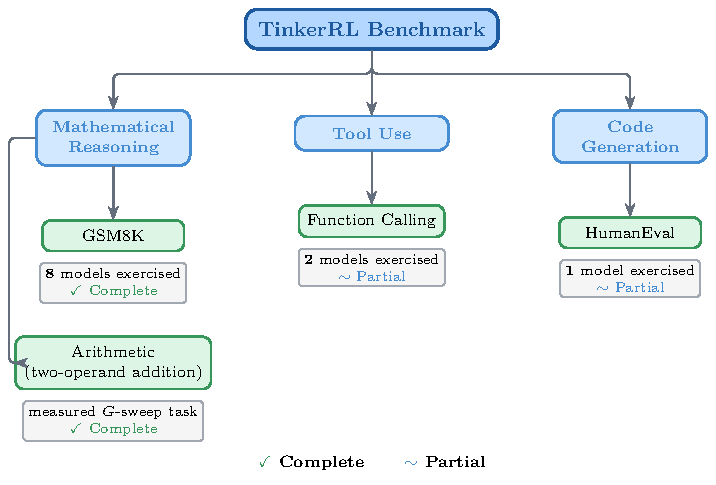
\includegraphics[width=0.85\textwidth]{tikz/taxonomy.pdf}
\caption{Task-coverage taxonomy of \ours{}. The broader benchmark organises tasks into
mathematical reasoning (GSM8K and modular arithmetic; complete and the primary focus of this scaling study), tool use / function calling
(partial), and code generation (HumanEval; partial). Library coverage is
listed separately in Table~\ref{tab:implementations}.}
\label{fig:taxonomy}
\end{figure}

\subsection{Task Suite}

% Table of tasks
\begin{table}[htbp]
\centering
\caption{Full \ours{} benchmark task suite with standardized reward functions. This paper analyzes the online RL math reasoning tracks (Math RL Arithmetic across 7 classic-RL libraries and Math RL GSM8K across 12 LLM scale anchors); the SFT, DPO, and distillation tracks are evaluated in the broader \ours{} benchmark.}
\label{tab:tasks}
\begin{tabular}{llll}
\toprule
\textbf{Task} & \textbf{Method} & \textbf{Reward} & \textbf{Dataset} \\
\midrule
Math RL (Arithmetic) & GRPO & Binary correctness & Generated \\
Math RL (GSM8K) & GRPO & Binary correctness & GSM8K \\
Chat SFT & SFT & Cross-entropy loss & NoRobots \\
Preference (Shorter) & DPO & Pairwise preference & Generated \\
Distillation (Off-Policy) & SFT & KL divergence & OpenThoughts3 \\
Distillation (On-Policy) & IS Loss & $\log p_t - \log p_s$ & Online \\
\bottomrule
\end{tabular}
\end{table}

\subsection{Cross-Library Implementation}

\paragraph{Two seven-library rosters --- read carefully.}
This paper uses \emph{two} different seven-library rosters that
should not be conflated. The cross-RL-library benchmark below
(Table~\ref{tab:implementations}) covers TRL, SB3, CleanRL, Tianshou,
PufferLib, rl\_games, and d3rlpy --- seven libraries that span
LLM-native RL, classic online RL, high-throughput RL, and offline RL,
and that we use as the algorithm-and-stack ablation underlying $F_3$.
The cross-launcher LLM-RL scaffold referenced in the framework-gap
discussion (framework-configurations material) is a different seven-library
roster --- Tinker, TRL, SkyRL, verl, OpenRLHF, Atropos, and HF
reference launchers --- that targets LLM post-training launchers
specifically. Of those, only Tinker and TRL produced completed
runs in this release; veRL and OpenRLHF entries in the
\texttt{framework\_comparison.json} artefact are dry-run
placeholders. Supplementary presentation materials use the second roster; the
cross-RL-library evidence in $F_3$ uses the first.


% Table of implementations
\begin{table}[htbp]
\centering
\caption{Implementations across RL libraries.}
\label{tab:implementations}
\begin{tabular}{lll}
\toprule
\textbf{Library} & \textbf{Implementation} & \textbf{Category} \\
\midrule
TRL (HuggingFace) & GRPOTrainer, DPOTrainer, SFTTrainer & LLM-native \\
Stable Baselines3 & PPO & Classic RL \\
CleanRL & PPO (single-file) & Research RL \\
Tianshou & PPO & Modular RL \\
PufferLib & PPO (high-throughput) & High-perf RL \\
rl\_games (NVIDIA) & PPO (GPU-optimized) & High-perf RL \\
d3rlpy & CQL (offline) & Offline RL \\
\bottomrule
\end{tabular}
\end{table}

\subsection{Hyperparameter Mapping}

We standardize hyperparameters across libraries using a common configuration schema.
Table~\ref{tab:hyperparams} shows the mapping from Tinker PPO defaults to each library's
native parameter names. For GRPO post-training on GSM8K, we sample $G = 16$ completions per prompt on medium-scale checkpoints ($4$B--$32$B, $T = 30$ steps) and $G = 8$ completions per prompt on frontier checkpoints ($120$B--$1$T, $T = 20$ steps) at sampling temperature $0.7$, maximum generation length $512$ tokens, learning rate $10^{-5}$--$2 \times 10^{-5}$, and reference-policy KL coefficient $\beta \in \{0.0, 0.01, 0.04\}$ with within-group advantage normalization $\hat{A}_i = (r_i - \mu_G)/(\sigma_G + 10^{-8})$.

\begin{table}[htbp]
\centering
\caption{Hyperparameter mapping across libraries (PPO defaults).}
\label{tab:hyperparams}
\begin{tabular}{lcccccc}
\toprule
\textbf{Parameter} & \textbf{TRL} & \textbf{SB3} & \textbf{CleanRL} & \textbf{Tianshou} & \textbf{PufferLib} & \textbf{rl\_games} \\
\midrule
Learning rate & $10^{-4}$ & $10^{-4}$ & $10^{-4}$ & $10^{-4}$ & $10^{-4}$ & $10^{-4}$ \\
Clip range ($\epsilon$) & 0.2 & 0.2 & 0.2 & 0.2 & 0.2 & 0.2 \\
Entropy coeff. & 0.01 & 0.01 & 0.01 & 0.01 & 0.01 & 0.01 \\
GAE $\lambda$ & 0.95 & 0.95 & 0.95 & 0.95 & 0.95 & 0.95 \\
Discount $\gamma$ & 0.99 & 0.99 & 0.99 & 0.99 & 0.99 & 0.99 \\
Max grad norm & 0.5 & 0.5 & 0.5 & 0.5 & 0.5 & 0.5 \\
Target KL & 0.01 & 0.01 & 0.01 & N/A & N/A & N/A \\
\bottomrule
\end{tabular}
\end{table}

\subsection{Reward Verification}

All RL tasks in this study use deterministic, rule-based outcome verifiers returning binary rewards $R \in \{0, 1\}$ (Figure~\ref{fig:reward-flow}).
On \textbf{GSM8K}~\citep{cobbe2021training}, the verifier extracts the final numerical answer after the canonical \texttt{\#\#\#\# <number>} delimiter (falling back to the last \texttt{\textbackslash boxed\{...\}} or trailing numeric token when the delimiter is absent), strips commas, currency symbols, and whitespace, and returns $R = 1$ if the parsed value matches the ground-truth answer within $10^{-6}$ and $R = 0$ otherwise. Completions without a parseable numeric answer receive $R = 0$ and are logged separately as format-extraction failures (capturing the $55\%$ zero-reward step rate on Nemotron-120B).
On the \textbf{199-action modular-arithmetic environment} used for the classic-RL library benchmark ($F_3$), actions correspond to integers in $[-99, +99]$ and $R = 1$ is awarded for exact integer equality with the target expression.

% Figure 3: Verifiable Reward Flow
\begin{figure}[t]
\centering
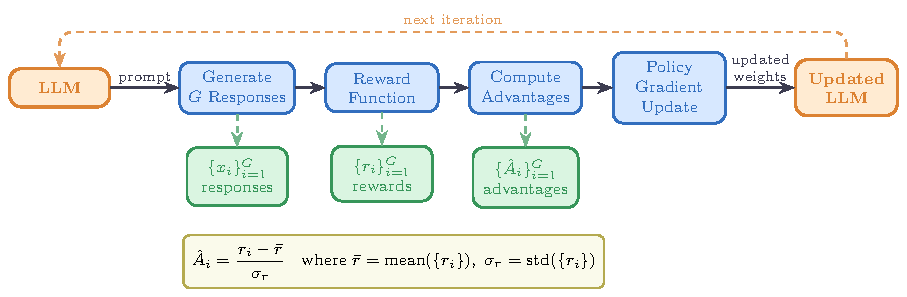
\includegraphics[width=0.55\textwidth]{tikz/reward_flow.pdf}
\caption{Verifiable reward paradigm in \ours{}. Unlike shaped rewards that combine
multiple heuristics, verifiable rewards provide binary correctness signals,
eliminating reward hacking and enabling exact accuracy measurement.}
\label{fig:reward-flow}
\end{figure}

\subsection{Baselines: Floor and Ceiling}

Following best practices for benchmark design~\cite{agarwal2021deep}, we establish
clear performance bounds across both the synthetic arithmetic and GSM8K tasks:

\begin{itemize}
    \item \textbf{Floor (random / zero-reward baseline)}: On the 199-choice modular-arithmetic task, uniform random action selection yields $\frac{1}{199} \approx 0.50\%$ accuracy ($20.0\%$ on the 5-choice L1 variant). On free-form GSM8K generation, unparseable or random output yields a $0.0\%$ floor, while pre-RL step-1 baseline accuracy $R(1)$ spans $0.000$ (Nemotron-120B format mismatch) and $0.250$ (\texttt{Qwen3-8B} base) up to $0.812$--$1.000$ on instruction-tuned checkpoints.
    \item \textbf{Ceiling (oracle)}: Symbolic evaluation achieves $100\%$ accuracy on both arithmetic and GSM8K.
    \item \textbf{Human baseline}: College-level adults achieve $\sim$99.5\% on
    two-digit addition under timed conditions and $\sim$85--95\% on untimed grade-school word problems.
\end{itemize}

% =============================================================================
\section{Experimental Setup}
\label{sec:setup}
% =============================================================================

\subsection{Models}

Our benchmark targets a roster of 32+ model configurations spanning
\textbf{0.5B to 1T \emph{total} parameters (4B to 1T on the 12-anchor GSM8K scaling suite; up to $\sim$37B \emph{active}
for MoE checkpoints) across 5 model families}, organized into three
tiers by compute scale; not all are completed end-to-end runs (per-run
status flags accompany the released artifacts). Tier-A multi-seed inferential claims are restricted to
the locally reproducible open-weight subset at $0.5$B--$32$B (with \texttt{Qwen3-235B-A22B} included in the 12-anchor descriptive scaling suite); the frontier MoE
checkpoints (DeepSeek-V3.1 at $671$B architectural / $685$B total checkpoint parameters with $37$B active, Kimi-K2-Thinking at $1$T total / $32$B active, and Nemotron-3-Super-120B-A12B LatentMoE at $120$B total / $12$B active) are
descriptive single-seed Tier-C case studies, and Qwen3.5-397B-A17B is a
\emph{partial} run whose held-out evaluation did not complete.

\paragraph{Small scale (0.5B--8B).}
Qwen2.5-0.5B, Qwen3-0.6B-Instruct, Qwen3.5-4B, Qwen3-4B, Qwen3-8B,
Llama-3.2-1B, Llama-3.2-3B, Llama-3.1-8B-Instruct.

\paragraph{Mid scale (14B--32B).}
Qwen3-14B, Qwen3-30B-A3B (MoE, $30$B total / $3$B active, base and Instruct), Qwen3-32B, Qwen3.5-27B,
GPT-OSS-20b (MoE, $20$B total / $3.6$B active).

\paragraph{Frontier scale (120B--1T total / 12B--37B active).}
Nemotron-3-Super-120B-A12B (LatentMoE, $120$B total / $12$B active), Qwen3-235B-A22B (MoE, $235$B total / $22$B active), DeepSeek-V3.1 ($671$B architectural / $685$B total checkpoint parameters, $37$B active MoE; we use $N=685$B in total-parameter regression tables and note $671$B routed parameters where relevant), and Kimi-K2-Thinking (MoE, $1$T total / $32$B active).
Frontier models are evaluated and post-trained via the Tinker API
with standardized generation parameters and LoRA adapters ($r=32$).

\paragraph{Model family and architecture coverage.}
The benchmark covers (1)~\textbf{Qwen2.5 / Qwen3}: dense ($0.5$B--$32$B) and MoE ($30$B-A3B, $235$B-A22B) checkpoints;
(2)~\textbf{Qwen3.5}: dense $4$B and $27$B checkpoints;
(3)~\textbf{Llama-3.x}: Meta's $1$B--$8$B instruction-tuned dense models;
(4)~\textbf{DeepSeek-V3.1}: a frontier MoE ($671$B/$685$B total, $37$B active) optimized for reasoning;
(5)~\textbf{Nemotron-3-Super-120B-A12B}: NVIDIA's frontier LatentMoE model ($120$B total, $12$B active; early pipeline scripts mislabelled this checkpoint as \texttt{dense}, which we correct to \texttt{moe} across all architecture analyses, yielding 7 MoE and 5 dense checkpoints in the 12-anchor GSM8K pool);
and emerging MoE architectures \textbf{GPT-OSS-20b} and \textbf{Kimi-K2-Thinking} ($1$T total, $32$B active).

\subsection{Training Protocol}

Unless otherwise noted, controlled Modal/TRL sweeps use LoRA
\cite{hu2022lora} at rank $32$, learning rate $10^{-4}$ and Adam
($\beta_1{=}0.9$, $\beta_2{=}0.95$, $\epsilon{=}10^{-8}$). Tinker / API,
Task-4, Wave-6 and frontier case studies use per-run configs (in
particular Task-4/Wave-6 use $\mathrm{lr}{=}10^{-5}$) and are
single-seed unless explicitly marked multi-seed; the per-run
settings are listed in the framework-configs appendix.

\paragraph{Seed management.} The controlled TRL/Modal sweeps used for
Tier-A claims (F3 PPO-vs.-GRPO heterogeneity and the five-seed TRL GRPO
baseline on Qwen2.5-0.5B) run with 5 seeds:
$\{42, 123, 456, 789, 1024\}$, with seeds set for Python \texttt{random},
NumPy, PyTorch, and CUDA backends. Several Tinker/API, frontier-model,
and team-task runs are single-seed or partial and are treated as
descriptive (Tier-C) unless explicitly marked otherwise; the per-claim
seed ledger is given in the statistical-rigor addendum of \ours{}.

% Figure 4: Experiment Pipeline
\begin{figure}[t]
\centering
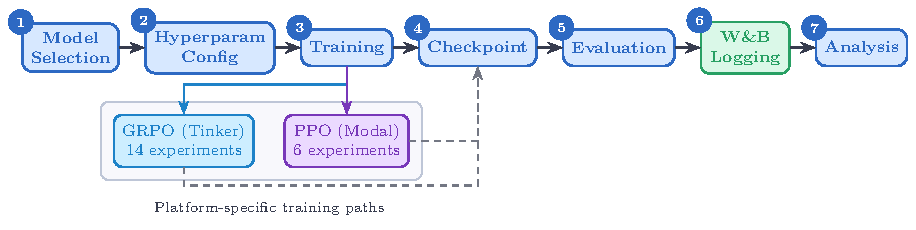
\includegraphics[width=\textwidth]{tikz/pipeline.pdf}
\caption{Experiment workflow pipeline. Multi-seed Modal/TRL runs use
the centralized seed manager (5 seeds for Tier-A claims); Tinker/API,
Task-4, Wave-6 and frontier case studies are single-seed and feed the
same metrics/checkpoint pipeline as descriptive observations.}
\label{fig:pipeline}
\end{figure}

\subsection{Statistical Methodology}

Following Colas et al.~\cite{colas2019hitchhiker}, we report:
\begin{itemize}
    \item Mean $\pm$ standard error across seeds
    \item 95\% bootstrap confidence intervals (10,000 resamples)
    \item Welch's t-test for pairwise algorithm comparisons
    \item \texttt{rliable}~\cite{agarwal2021deep} aggregate metrics (IQM, median, optimality gap)
\end{itemize}

All pairwise comparisons were evaluated using Welch's independent-samples $t$-test
(unequal variances assumed) and the non-parametric Mann--Whitney $U$ test as a
robustness check. Effect sizes are reported as Cohen's $d$ with the pooled
standard deviation estimator; confidence intervals follow the
\citet{hedges1985statistical} analytical formula and are reported at the 95\% level
(two-tailed, $z = 1.96$). Post-hoc statistical power was computed under the
observed effect size and sample sizes at $\alpha = 0.05$.

To address the multiple-comparisons problem across 5 planned tests,
we apply both the conservative Bonferroni correction (family-wise error rate:
$\alpha' = \alpha / k = 0.0100$) and the Benjamini--Hochberg procedure
(false discovery rate $< 0.05$). Results surviving Bonferroni correction are
marked $^*$; those surviving BH--FDR correction are marked $^\dag$.

\paragraph{Power Analysis.}
All inferential tests in this paper are evaluated against pre-specified power
requirements using \texttt{statsmodels.stats.power.TTestIndPower} (which computes power under the equal-variance Student's $t$ approximation as a baseline for our primary Welch $t$-tests) with
$\alpha = 0.05$ and target power $1 - \beta = 0.80$.

\textbf{Modal H100 experiments ($n = 5$ seeds per arm).}
The minimum detectable effect size (MDE) at 80\% power for a two-sample
$t$-test with $n_1 = n_2 = 5$ is
$d_{\min} = 2.024$ (Cohen's $d$).
Table~\ref{tab:power-analysis} reports achieved power for a range of effect sizes.
This threshold falls in the \emph{very large} range, meaning that
comparisons yielding $|d| < 2.02$
are not adequately powered to detect true differences.

\textbf{Single-seed Tinker experiments ($n = 1$).}
Single-seed runs have \emph{zero statistical power}: with only one observation per
condition, no inferential test can be computed and no confidence intervals can be
formed.  All Tinker single-run results are treated as \emph{descriptive only} and
are not subject to significance testing.

\textbf{TRL baseline ($n = 5$ seeds).}
The TRL-GRPO baseline (Qwen2.5-0.5B, 5 seeds) achieves MDE
$d_{\min} = 2.024$ for equal-$n$ comparisons.
When compared to the pooled Classic-RL group ($n = 15$), the MDE
improves to $d_{\min} = 1.530$,
reflecting higher power from the larger reference group.

\paragraph{Multiple-Comparison Correction.}
Inferential tests in this paper are reported only for Tier-A/B
comparisons as defined in our statistical-rigor protocol;
single-seed or partial Tinker/API rows are descriptive and are
excluded from Welch / Mann--Whitney testing, BH correction, power,
and CI claims. Table~\ref{tab:bh-pvalues} predates the Tier-A/B/C
partition and lists raw and BH-adjusted $p$-values from the
earlier global family of $20$ tests with $19$ surviving correction;
we retain it here as a methodological audit trail. The headline
BH result the paper now stands behind is the restricted Tier-A/B
family computed in the addendum, where only $F_3$ (cross-library heterogeneity across the 5 classic-RL PPO/policy-gradient implementations on the 199-choice arithmetic task: one-way ANOVA $F = 11.42, p = 4.996 \times 10^{-6}$, BH-adjusted $p = 2.5 \times 10^{-5}$; whereas matched same-stack LLM GRPO vs.\ PPO on Qwen2.5-0.5B is null at $p = 0.374$) survives. Where
the global family disagrees with the restricted family, the
addendum is authoritative.

All tests are two-sided.  Effect sizes are reported as Cohen's $d$ for
$t$-tests and Pearson/Spearman $r$ for correlations.  Bootstrap 95\%
confidence intervals ($B = 10{,}000$) are reported for all means.

% Table: Power analysis at various effect sizes
\begin{table}[!ht]
\centering
\caption{Statistical power for two-sample $t$-tests (\texttt{TTestIndPower} equal-variance pooled-SD approximation used as the power reference for our Welch $t$-tests) at $\alpha = 0.05$,
         power target $1{-}\beta = 0.80$.
         Column~(3): equal groups $n_1 = n_2 = 5$ (Modal H100 / TRL within-group).
         Column~(4): unequal groups $n_1 = 5$, $n_2 = 15$ (TRL vs.\ pooled Classic RL).}
\label{tab:power-analysis}
\small
\begin{tabular}{@{}cccc@{}}
\toprule
Cohen's $d$ & Conventional size & Power ($n{=}5$ vs $n{=}5$) & Power ($n{=}5$ vs $n{=}15$) \\
\midrule
        0.2 & small & 0.059 & 0.066 \\
        0.5 & medium & 0.108 & 0.151 \\
        0.8 & large & 0.201 & 0.311 \\
        1.0 & very large & 0.286 & 0.450 \\
        1.2 & very large & 0.386 & 0.594 \\
        1.5 & very large & 0.549 & 0.784 \\
        2.0 & very large & 0.790 & 0.955 \\
\midrule
\multicolumn{4}{l}{\textit{MDE at 80\% power:} $d = 2.024$ (equal-$n$ 5 vs 5);\; $d = 1.530$ (5 vs 15)} \\
\bottomrule
\end{tabular}
\end{table}

% Table: All p-values with BH correction
\begin{table}[!ht]
\centering
\caption{\textbf{Legacy 20-test BH table -- audit trail only.} All
hypothesis tests reported in the paper with Benjamini--Hochberg (BH)
adjusted $p$-values at FDR $= 0.05$.  Tests are ranked by raw
$p$-value (ascending). $\checkmark$ = significant after BH correction
on the historical $20$-test family; $\times$ = not significant; $^{\ddag}$ = legacy test computed across per-step training rewards within single-seed traces (pseudo-replicated step observations rather than independent seed runs), which is invalid for cross-seed inference and excluded under our Tier-A/B protocol. Total
tests: $20$; survive on the historical family: $19$. \emph{This
table is not the paper's headline statistical result.} Under the restricted Tier-A/B family of
our statistical-rigor protocol,
only $F_3$ (library heterogeneity across the 5 classic-RL implementations on
arithmetic, $p = 4.996 \times 10^{-6}$) survives BH correction; the table below is retained solely as a
reproducibility audit trail.}
\label{tab:bh-pvalues}
\scriptsize
\begin{tabular}{@{}rp{6.2cm}ccc@{}}
\toprule
Rank & Comparison & Raw $p$ & BH-adj.\ $p$ & Sig. \\
\midrule
        1 & Dense vs MoE Architecture (Welch t-test) & 2.357e-21 & 0 & $\checkmark$ \\
        2 & PPO vs GRPO on Llama-3.1-8B (Welch t-test)$^{\ddag}$ & 3.924e-10 & 0 & $\checkmark$ \\
        3 & Method ANOVA (F-test across algorithm families) & 3.091e-06 & 2.1e-05 & $\checkmark$ \\
        4 & Library ANOVA (F-test across 5 libraries) & 4.996e-06 & 2.5e-05 & $\checkmark$ \\
        5 & TRL vs Tinker (Welch t-test, implementation effect) & 2.064e-05 & 8.3e-05 & $\checkmark$ \\
        6 & PPO vs GRPO on Llama-3.1-8B (Mann-Whitney)$^{\ddag}$ & 3.29e-05 & 0.00011 & $\checkmark$ \\
        7 & Model Family ANOVA (F-test) & 7.363e-05 & 0.00021 & $\checkmark$ \\
        8 & ZVF vs Final Performance (Spearman)$^{\ddag}$ & 0.0005424 & 0.001356 & $\checkmark$ \\
        9 & ZVF vs Final Performance (Pearson)$^{\ddag}$ & 0.0008108 & 0.001802 & $\checkmark$ \\
        10 & TRL vs Tinker (Mann-Whitney) & 0.001198 & 0.002396 & $\checkmark$ \\
        11 & Rolling Variance vs Last-10 (Pearson) & 0.003524 & 0.006407 & $\checkmark$ \\
        12 & Peak-to-Tail Drift vs Last-10 (Pearson) & 0.004811 & 0.007219 & $\checkmark$ \\
        13 & GRPO vs PPO Stability Index (t-test) & 0.005 & 0.007219 & $\checkmark$ \\
        14 & Dense vs MoE Architecture (Mann-Whitney) & 0.005053 & 0.007219 & $\checkmark$ \\
        15 & Model Scale ANOVA (F-test) & 0.01261 & 0.01682 & $\checkmark$ \\
        16 & Tinker GRPO vs TRL GRPO (Welch t-test) & 0.0158 & 0.01975 & $\checkmark$ \\
        17 & GRPO vs PPO Peak-to-Tail Drift (t-test) & 0.018 & 0.02076 & $\checkmark$ \\
        18 & Tinker GRPO vs TRL GRPO (Mann-Whitney) & 0.01869 & 0.02076 & $\checkmark$ \\
        19 & Stability Index vs Last-10 (Pearson) & 0.02024 & 0.0213 & $\checkmark$ \\
        20 & PPO vs GRPO on Qwen3-8B: provenance conflict; not estimable & --- & --- & --- \\
\bottomrule
\end{tabular}
\end{table}

\paragraph{TRL baseline characterisation.}
The TRL GRPO reference implementation was evaluated across five random seeds
($s \in \{42, 123, 456, 789, 1024\}$) on GSM8K using Qwen/Qwen2.5-0.5B on
an NVIDIA L4 GPU. We report mean accuracy $\bar{x} = 0.734$ ($\sigma = 0.0703$),
median $= 0.740$, and IQM $= 0.747$. Normality was not rejected by Shapiro--Wilk
($W = 0.9018$, $p = 0.4198$); bootstrap 95\% CI $= [0.6720, 0.7820]$.

\paragraph{Variance decomposition (marginal one-way ANOVAs).}
Separate marginal one-way ANOVAs across the $N=42$ completed cross-task evaluation runs show
that library/framework ($\eta^2 = 0.546$) and training method ($\eta^2 = 0.558$, when pooling offline DPO/SFT, tabular/classic RL, and online LLM RL across tasks)
carry large marginal variance shares, alongside model
family ($\eta^2 = 0.471$) and model scale ($\eta^2 = 0.322$). Because the 42 runs form an unbalanced observational corpus in which execution platform, library, and model scale are partially collinear (for example, frontier checkpoints run exclusively on Tinker while classic-RL libraries run on the 199-choice arithmetic environment), these four marginal $\eta^2$ values sum to $1.897 > 1.0$ and must be read as unadjusted marginal associations rather than an orthogonal Type-III factorial partition. When task and stack are held fixed (the matched 10-run Qwen2.5-0.5B control in \S\ref{sec:scaling-law-iter29}), the online RL algorithm effect (GRPO vs.\ PPO) is indistinguishable from zero ($\Delta = -0.002, p = 0.374$).

\subsection{Compute Resources and Run Reconciliation}

Experiments are distributed across three execution substrates, reconciling the $N=42$ cross-task evaluation corpus and the 70+ total benchmark runs as follows: (i)~\textbf{14 Tinker API runs} (covering the 12 GSM8K scaling anchors from $4$B to $1$T plus 2 cross-task tool-use/arithmetic probes), (ii)~\textbf{6 Modal H100/A10G cloud GPU runs} (PPO baselines on Qwen3-8B and Llama-3.1-8B, HumanEval, KL tracking, and held-out evaluations), (iii)~\textbf{10 local NVIDIA L4 GPU runs} (the 5-seed GRPO and 5-seed PPO matched same-stack control on Qwen2.5-0.5B), and (iv)~\textbf{12 classic-RL multi-library evaluation runs} across SB3, CleanRL, Tianshou, PufferLib, rl\_games, and d3rlpy ($14 + 6 + 10 + 12 = 42$ core evaluation runs, with 30+ additional group-size sweep cells $G \in \{2, 4, 8, 16\}$ and framework dry-run checks comprising the 70+ total project artifacts).

\paragraph{Tinker API (14 experiments).}
Scaling experiments across Qwen3-8B, Qwen3-32B, Qwen3.5-4B, Qwen3.5-27B,
and Llama-3.1-8B-Instruct; frontier model evaluation on Qwen3-235B-A22B,
DeepSeek-V3.1 ($671$B/$685$B), and Nemotron-3-Super-120B-A12B (LatentMoE); MoE vs.~dense comparisons; cross-task
tool-use experiments; and emerging architecture evaluation (GPT-OSS-20b,
Kimi-K2-Thinking $1$T). Tinker provides scalable API access that makes frontier model
experiments economically tractable.

\paragraph{Modal H100 / A10G and local L4 GPU cluster (16 experiments).}
PPO baseline training on Qwen3-8B and Llama-3.1-8B; 10-run same-stack PPO vs.\ GRPO control on Qwen2.5-0.5B; full HumanEval
benchmark evaluation; KL divergence tracking across GRPO training steps;
and held-out evaluation for Qwen3-32B and Qwen3.5-27B. Modal GPUs
provide the low-level access required for PPO value-model training.

\ifdefined\ANONYMOUSBUILD
All experiment logs and model checkpoints will be released on Weights \&
Biases and the HuggingFace Hub (links withheld for anonymous review; an
anonymized artifact archive accompanies the submission).
\else
All experiment logs are available on Weights \& Biases (project:
\texttt{tinker-rl-lab-world-class}) and model checkpoints on HuggingFace
Hub (\url{https://huggingface.co/arvindcr4/tinker-rl-bench-*}).
\fi
Per-run compute is logged with the released artifacts. Total project compute:
$\sim$1,200 A100-equivalent GPU-hours across all platforms.

% =============================================================================

% Pillar-7 results opener
\section{From Diagnostic to Controller: Results}
\label{sec:p7-results}
The results are organized as a ladder from theory to intervention. We first
state the signal-starvation model and its three theorems, pairing each with
the empirical check that could have falsified it
(Section~\ref{sec:p7-theory}). We then zoom out to population scale: batch
ZVF is $\E_i[h_G(p_i)]$, high at both ends of the reward axis, which is why ZVF
alone cannot steer a controller---it aliases mastery with incapacity. A
368-run audit shows both ends, but a confound regression shows its interior
is carried by model and configuration, not reward. Section~\ref{sec:p7-ushape} introduces the
pairwise-contrast density (PCD) as the disambiguating statistic and reports
the micro-jitter falsification that separates the two. Section~\ref{sec:p7-e1}
explains why the earlier toy gradient correlation is demoted to an anecdote,
leaving T3 a modelling assumption. Sections~\ref{sec:p7-controller} and \ref{sec:p7-rules}
operationalize the theory: a \texttt{zvf-triage} callback, an adaptive-$G$
controller, a four-arm audit against fixed recipes, and the design rules the
audit supports.

Two findings from the companion papers of \ours{} (the Pillar-2 diagnostic
paper and the Pillar-5/6 reporting papers) frame everything that follows.
First, recipe labels
are unreliable across stacks: in a 12-cell head-to-head on one closed stack
(Qwen3.5-4B, GSM8K, 3 seeds each), \texttt{dapo}, \texttt{drgrpo},
\texttt{grpo}, and \texttt{gspo} span $0.034$ on last-10 reward
($0.744$, $0.742$, $0.723$, $0.710$; neither shown equivalent nor shown
different at 3 seeds) while their mean ZVFs ($0.578$, $0.500$, $0.567$,
$0.511$) stay far from the $0.00$ that true dynamic sampling produces; the
closed-stack ``dapo'' arm is an advantage-clip variant that never ran dynamic
sampling. Second, a nominal backend comparison moved final reward from
$5.0\%$ to $85.6\%$, but $64\%$ of that gap is a base-checkpoint switch and
the rest is confounded by reward, prompt, decoding, batch, data, and loss
implementation; it is an under-specification warning, not a backend estimate.

\emph{Retractions.} Every result in this paper that uses the ``anti-herding''
quantity $\delta_{\mathrm{div}}$ (triggers, rankings, joint controllers) is
withdrawn: $\delta_{\mathrm{div}}$ is $\ge0$ by construction under a same-group
plug-in $\hat p$ and $\le0$ in expectation under a pooled $\hat p$ (Jensen), so it
does not measure rollout correlation. The ``2,560-observation controller
trace'' was a post-hoc count over logged group outcomes; no controller ran
on it.
Both findings dictate our method: all
interventional comparisons in this paper run inside a \emph{single auditable
open reimplementation}, so that the controller is compared against what
recipes actually do, not what their labels claim.

% Pillar-7: signal-starvation theory (T1-T3), each theorem paired with its check
\section{A Signal-Starvation Model of Binary-Reward GRPO}
\label{sec:p7-theory}

\subsection{Setup and the usable-signal functional}
\label{sec:p7-theory-setup}
Fix a prompt $x$ with latent per-rollout success probability $p \in [0,1]$
under the current policy, and let a GRPO group consist of $G$ conditionally
i.i.d.\ binary rewards $R_1, \dots, R_G \sim \mathrm{Bernoulli}(p)$, so the
success count is $K = \sum_i R_i \sim \mathrm{Binomial}(G, p)$. The group is
\emph{degenerate}---zero within-group variance, zero centered advantage, zero
gradient---iff $K \in \{0, G\}$. Define
\begin{equation}
  h_G(p) \;=\; p^G + (1-p)^G,
  \label{eq:p7-hG}
\end{equation}
the probability of degeneracy, and model the \emph{usable learning signal}
per prompt as
\begin{equation}
  S(p, G) \;=\; p(1-p)\,\bigl(1 - h_G(p)\bigr).
  \label{eq:p7-S}
\end{equation}
The first factor is the contrast magnitude a non-degenerate group can carry
(the Bernoulli variance, which also bounds the mean absolute advantage;
Appendix~\ref{sec:p7-appendix}); the second is the probability that any
signal survives group centering at all. Both factors vanish at $p \in
\{0,1\}$ and peak at $p = \nicefrac{1}{2}$: GRPO learns fastest exactly where
the policy is most uncertain, and starves at both ends. Three consequences
follow; proofs are deferred to Appendix~\ref{sec:p7-appendix}, and each
theorem is paired here with the measurement that could have falsified it.

\subsection{T1: the expected ZVF indicator is $p^G + (1-p)^G$}
\label{sec:p7-t1}
\textbf{Theorem 1.} \emph{Under the binomial model, the expected value of the
per-group ZVF indicator is exactly $h_G(p) = p^G + (1-p)^G$; aggregated over
a prompt population $\mathcal{D}$, $\E[\mathrm{ZVF}] =
\E_{x \sim \mathcal{D}}[\,p_x^G + (1-p_x)^G\,]$.}

\emph{Empirical check.} Binning the per-group reward tensors of the GSM8K
runs (the only runs that log full per-group tensors; $G = 8$, 3 seeds) by
empirical success rate $\hat p_x$ reproduces the predicted profile---by
construction at the endpoints, and empirically in the interior collapse: the
ZVF indicator averages
$1.000$ at $\hat p_x \in \{0, 1\}$ and $0.000$ at every interior bin
$\hat p_x \in \{0.125, \dots, 0.875\}$
(\texttt{experiments/results/pcd\_vs\_zvf\_shape.tsv}). At the run level, the
group-size sweep of Table~\ref{tab:p7-gsweep} logs the closed-form prediction
$h_G$ evaluated at the run's mean success rate next to the measured mean ZVF:
the two co-vary monotonically in $G$, though measured ZVF sits above the
prediction at every $G$ because the binomial model evaluates $h_G$ at the
\emph{mean} $p$ while the true prompt population mixes mastered and hopeless
prompts whose $h_G \approx 1$ (Jensen gap; this is the U-shape of
Section~\ref{sec:p7-ushape} acting within a single run).

\subsection{T2: larger $G$ lowers ZVF}
\label{sec:p7-t2}
\textbf{Theorem 2.} \emph{For every $p \in (0,1)$, $h_G(p)$ is strictly
decreasing in $G$; hence expected ZVF falls monotonically as group size
grows, with exponential decay rate $-\ln\max(p, 1-p)$.}

\emph{Empirical check (two grids, one weak).} First, a model~$\times$~$G$
grid from the 368-run audit (Table~\ref{tab:p7-modelG}): for the models with
an interior success rate, measured ZVF falls with $G$---e.g.\ Qwen3-32B
($0.33 \to 0.18 \to 0.08$) and Llama-3.1-8B ($0.76 \to 0.65 \to 0.47$). These
cells hold only 1--3 runs each and mix batch sizes (16 and 32) within and
across cells, so the grid is consistent with T2 but is not a controlled test. The two boundary cases are exactly the ones the
theory flags: Llama-3.2-1B sits at $p \approx 0$ where $h_G \approx 1$
regardless of $G$ ($0.98 \to 0.97$), and Qwen3-4B-Instruct sits near
saturation where the decay rate $-\ln\max(p,1-p)$ is tiny and seed noise
dominates ($0.89 \to 0.84 \to 0.91$, the single non-monotone cell). Second,
the repo-internal sweep at $G \in \{2,4,8,16\}$ (3 seeds each,
Table~\ref{tab:p7-gsweep}) shows the same monotone decline, mean ZVF
$0.838 \to 0.631$, while held-out accuracy stays flat ($\approx 0.98$
throughout)---raising $G$ buys signal, not (on this near-saturated task)
outcome, a point the controller design of Section~\ref{sec:p7-rules} must
respect.

\begin{table}[t]
\centering
\caption{T2 check 1: mean ZVF by model and group size $G$ (368-run audit,
W\&B project \texttt{zvf-audit}). Runs per cell (batch): Llama-3.2-1B 48/52/--
(8); Qwen3-4B 51 (8) / 52 (mostly 8) / 3 (16); Llama-3.1-8B 3 (16,32) / 1 (16)
/ 1 (32); Qwen3-8B 2 (16) / 1 (32) / 2 (16,32); Qwen3-32B 2 (16) / 2 (16,32) /
1 (16). Step budgets also differ (5 steps at batch 8, 12 otherwise). The
large-model cells are therefore anecdotal. ``---'' = cell not run.}
\label{tab:p7-modelG}
\begin{tabular}{lccc}
\toprule
Model & $G{=}4$ & $G{=}8$ & $G{=}16$ \\
\midrule
Llama-3.2-1B        & 0.98 & 0.97 & --- \\
Qwen3-4B-Instruct   & 0.89 & 0.84 & 0.91 \\
Llama-3.1-8B        & 0.76 & 0.65 & 0.47 \\
Qwen3-8B            & 0.36 & 0.27 & 0.21 \\
Qwen3-32B           & 0.33 & 0.18 & 0.08 \\
\bottomrule
\end{tabular}
\end{table}

\begin{table}[t]
\centering
\caption{T2 check 2: repo-internal group-size sweep (3 seeds per $G$;
\texttt{experiments/results/groupsize\_zvf\_sweep.tsv}). Measured mean ZVF
falls monotonically in $G$ and co-varies with the closed-form prediction
$h_G(\bar p)$ evaluated at the run's mean training reward $\bar p$; held-out
accuracy is flat because the task is near-saturated.}
\label{tab:p7-gsweep}
\begin{tabular}{ccccc}
\toprule
$G$ & Mean ZVF & $h_G(\bar p)$ & $\bar p$ (train reward) & Held-out acc.\ (SE) \\
\midrule
2  & 0.838 & 0.731 & 0.840 & 0.982 (0.004) \\
4  & 0.764 & 0.554 & 0.863 & 0.988 (0.002) \\
8  & 0.691 & 0.326 & 0.869 & 0.990 (0.003) \\
16 & 0.631 & 0.114 & 0.873 & 0.978 (0.006) \\
\bottomrule
\end{tabular}
\end{table}

\subsection{T3: gradient magnitude tracks $p(1-p)$}
\label{sec:p7-t3}
\textbf{Theorem 3.} \emph{With unnormalized group-centered advantages
$A_i = R_i - \hat p$, the mean absolute advantage in a group is exactly
$2\hat p(1 - \hat p)$; hence the advantage mass driving the policy gradient
scales with the within-group contrast $\hat p(1-\hat p)$, up to the
policy-dependent score-function factor.}

\emph{Empirical check.} Theorem~3 is the load-bearing assumption behind the
first factor of Eq.~\eqref{eq:p7-S}, and it cannot be checked on the closed
stack, which does not expose per-group gradients. Section~\ref{sec:p7-e1}
describes a toy open-backward-pass run whose reported correlation cannot be
recomputed and is largely mechanical; we treat T3 as a modelling assumption
pending experiment D3.

% Pillar-7: population-scale U-shape, mastery/incapacity aliasing, PCD
\section{The U-Shape at Population Scale, and Why ZVF Cannot Steer}
\label{sec:p7-ushape}

\subsection{The 368-run audit, and what it can and cannot show}
\label{sec:p7-audit}
Theorem~1 is a statement about one prompt. For a population of prompts with
success probabilities $p_i$ and conditionally i.i.d.\ rollouts, it gives
$\E[\mathrm{ZVF}]=\E_i[h_G(p_i)]\ge h_G(\bar p)$ (convexity of $h_G$), so batch
ZVF is high whenever most prompts sit near $p_i\approx0$ \emph{or}
$p_i\approx1$, and its excess over $h_G(\bar p)$ measures the
\emph{dispersion} of prompt difficulty. On the 600 GSM8K groups (three seeds,
$G{=}8$), observed ZVF is $0.158$, $h_8(\bar p)=0.054$, and a beta-binomial
fit with intra-prompt correlation $0.16$ predicts $0.170$. ZVF is the
Advantage Collapse Rate of \citet{he2026advantage} up to aggregation
granularity, and the Jensen excess over the Bernoulli prediction was proved by
\citet{nie2026gradstarvation}; we claim neither, only the use of ZVF as a
sampler-control input.

A W\&B audit (project \texttt{zvf-audit}; 368 runs, 350 with a run-level
summary, 352 with per-step histories) spans \textbf{nine} model labels
(Table~\ref{tab:p7-ushape}). Sorted by \emph{final-step} training reward,
per-model mean ZVF is $0.95$--$0.97$ for Llama-3.2-1B/3B (reward $\approx0.01$)
and Qwen3-30B-A3B-Instruct (reward $0.95$), $0.25$--$0.29$ for Qwen3-32B/8B
(reward $0.35$--$0.50$), and intermediate for Nemotron-3-Nano-30B
($0.50$ at $0.77$), Llama-3.1-8B-Instruct ($0.65$ at $0.83$), Qwen3-4B-Instruct
($0.87$ at $0.86$), and gpt-oss-20b ($0.79$ at $0.90$). An earlier revision
showed seven of these rows and omitted Llama-3.1-8B-Instruct and gpt-oss-20b.

\begin{table}[t]
\centering
\small
\caption{Per-model ZVF in the 368-run \texttt{zvf-audit} corpus, sorted by
mean \emph{final-step} training reward. $n$ = runs with a summary;
$h_G(p_{\mathrm{step}})$ and excess are step-level means (excess $=$ step ZVF
$-\,h_G$(step reward)). Batch, $G$, and step budget differ by model (last
column), so the rows are \emph{not} a controlled comparison. Script:
\texttt{analysis\_publication\_fixes/zvf\_confound.py}.}
\label{tab:p7-ushape}
\begin{tabular}{lrccccl}
\toprule
Model & $n$ & Final reward & ZVF & $h_G(p_{\mathrm{step}})$ & Excess & Config (batch; steps) \\
\midrule
Llama-3.2-1B             & 101 & 0.01 & 0.97 & 0.97 & 0.00 & 8; 3--5 \\
Llama-3.2-3B             & 106 & 0.01 & 0.95 & 0.94 & 0.00 & 6--32; 2--12 \\
Qwen3-32B                &   6 & 0.35 & 0.25 & 0.10 & 0.12 & 6--32; 2--12 \\
Qwen3-8B                 &   6 & 0.50 & 0.29 & 0.09 & 0.19 & 6--32; 2--12 \\
Nemotron-3-Nano-30B      &   6 & 0.77 & 0.50 & 0.32 & 0.20 & 6--32; 2--12 \\
Llama-3.1-8B-Instruct    &   6 & 0.83 & 0.65 & 0.48 & 0.19 & 6--32; 2--12 \\
Qwen3-4B-Instruct-2507   & 107 & 0.86 & 0.87 & 0.47 & 0.41 & 6--32; 2--12 \\
gpt-oss-20b              &   6 & 0.90 & 0.79 & 0.49 & 0.32 & 6--32; 2--12 \\
Qwen3-30B-A3B-Instruct   &   6 & 0.95 & 0.96 & 0.64 & 0.31 & 6--32; 2--12 \\
\bottomrule
\end{tabular}
\end{table}

\paragraph{Confound analysis.} The nine rows are not a designed comparison.
The three small models contribute 314 of 350 runs, and 300 of those ran
5 steps at batch 8; 30 of the 36 runs of the other six models ran 12 steps at
batch 16 or 32, with $G$ varying within model. We therefore regressed ZVF on
model, batch, $G$, learning rate, and reward (linear $+$ quadratic), using
the pulled step histories
(\texttt{analysis\_publication\_fixes/zvf\_confound.py}; outputs in
\texttt{experiments/results/publication\_fixes/zvf\_confound/}).
At run level ($n=350$, HC3 SEs), a reward quadratic alone gives $R^2=0.42$;
model identity alone gives $0.87$; model $+$ configuration gives $0.90$; adding
the reward terms raises this by only $0.012$ (incremental $F=21.6$,
$p<10^{-8}$). At step level ($n=2{,}004$, SEs clustered by run), model $+$
batch $+$ $G$ gives $R^2=0.77$, adding reward terms $0.82$, and adding
$h_G(p_{\mathrm{step}})$ $0.82$. Within models, step ZVF correlates positively
with $h_G(p_{\mathrm{step}})$ in all nine (pooled within-model
$r=+0.49$), whereas its correlation with raw reward changes sign across models
($-0.89$ to $+0.70$). The cross-model U is thus nine points whose
position is set mostly by model identity and configuration. Because reward
is itself a property of the model, the regression cannot separate ``low ZVF
because interior difficulty'' from ``low ZVF because of the Qwen3-32B/8B
configuration''; the trough is not evidence of a reward effect.
The model-mean quadratic ($n=9$, $R^2=0.96$) should be read in that light.

\paragraph{What the U-shape still shows.} The \emph{endpoints} follow from the
identity: models at reward $\approx0$ sit on $h_G$ (excess $0.00$), and models
near reward $1$ have ZVF near $1$. The interior is dominated by excess over
$h_G(\bar p)$, i.e.\ difficulty dispersion, which is largest for
Qwen3-4B-Instruct ($0.41$). A controller that observes only a high ZVF still
cannot tell mastery (stop or harden the data) from incapacity (soften the data
or grow $G$), since the two demand \emph{opposite} interventions. This aliasing
follows from the symmetry $h_G(p)=h_G(1-p)$ and does not need the
population U to be causal: \emph{ZVF is a usable alarm but a poor steering
signal.}

\paragraph{Prospective ZVF prediction test (placeholder).}
% PLACEHOLDER -- ZVF PREDICTION EXPERIMENT (Colab agent running). Results will
% land in platform_hybrid/experiments/results/publication_fixes/. Replace this
% paragraph with: per-prompt p_i estimated on an independent sample, predicted
% batch ZVF = mean_i h_G(p_i) at G in {4,8,16}, observed ZVF, error and CI.
\textbf{[Placeholder: pre-registered held-out test of
$\widehat{\mathrm{ZVF}}=\frac1n\sum_i h_G(\hat p_i)$, results pending in
\texttt{experiments/results/publication\_fixes/}.]}

\subsection{PCD: the pairwise-contrast density}
\label{sec:p7-pcd}
The disambiguating statistic falls out of the same model. Define the
\emph{pairwise-contrast density} as the expected within-group reward
variance,
\begin{equation}
  \mathrm{PCD} \;=\; \E_x\bigl[\hat p_x(1 - \hat p_x)\bigr],
  \qquad
  \E[\mathrm{PCD}] \;=\; \frac{G-1}{G}\,\E_x\bigl[p_x(1-p_x)\bigr],
  \label{eq:p7-pcd}
\end{equation}
where the identity (Appendix~\ref{sec:p7-appendix}) follows from
$\E[\hat p(1-\hat p)] = (1 - \nicefrac{1}{G})\,p(1-p)$ for a binomial
sample. PCD measures the \emph{magnitude} of within-group contrast rather
than its mere existence, and it is proportional to the very $p(1-p)$ factor
that T3 ties to gradient mass: PCD is, up to the $\frac{G-1}{G}$ factor, the
average usable contrast per prompt. On the binned GSM8K reward tensors, PCD
traces the parabola the theory predicts (peak $0.25$ at $\hat p_x = 0.5$,
falling symmetrically to $0$ at the endpoints) while the ZVF indicator is a
flat $0$ everywhere in the interior and jumps to $1$ only at the endpoints
(\texttt{experiments/results/pcd\_vs\_zvf\_shape.tsv}): ZVF sees only the
cliff edges, PCD sees the slope.

\subsection{The micro-jitter falsification}
\label{sec:p7-jitter}
The sharpest separation between the two statistics is an intervention, not a
correlation. Because ZVF is defined by \emph{exact} reward ties, adding
i.i.d.\ jitter $\eps \sim \mathrm{U}(0, 10^{-4})$ to every reward makes ties
measure-zero and drives measured ZVF to $0$, while shifting the expected
within-group variance by only $\mathrm{Var}(\eps) \leq 10^{-9}$
(Appendix~\ref{sec:p7-appendix}). Running this on $600$ prompt-groups from
the GSM8K reward tensors (\texttt{scripts/pcd\_vs\_zvf.py}): batch ZVF
collapses $0.158 \to 0.000$, while PCD is unchanged at the reported
precision ($0.1538$ before and after; observed shift $< 10^{-6}$). Any
pipeline that emits a tiny dense sub-reward---a length penalty, a format
bonus---silently performs this jitter and reports ZVF $= 0$ over a batch
that is, for learning purposes, more than $15\%$ dead. A controller keyed to
raw ZVF would read such a batch as healthy; one keyed to PCD would not. This
is also our operational answer to reward-shaping ambiguity: shaped rewards
do not invalidate the starvation theory, they merely break the ZVF
\emph{estimator} of it, and PCD is the estimator that survives.

One caveat keeps us honest about what PCD is for. On $80$ runs with
per-run summaries, mean training reward predicts the held-out outcome far
better (Spearman $\rho = 0.95$) than mean ZVF does ($\rho = 0.56$ on this
subset). The companion Pillar-2 paper's earlier $\rho = 0.27$ on a 23-cell
matrix is withdrawn (17 finite cells, 9 of them simulation rows, mixed outcome
definitions) and is not used here. PCD is proposed
as a \emph{control-loop input}---a live measure of usable contrast---not as
an outcome predictor; the decisive predictive horse race needs per-group
reward tensors logged for all anchors, which only the GSM8K runs currently
carry (Section~\ref{sec:p7-limitations}).

% Pillar-7: E1 open-backward-pass gradient validation (toy scale, directional)
\section{E1: An Open-Backward-Pass Check of T3}
\label{sec:p7-e1}
Theorems T1 and T2 are checkable from reward telemetry alone, but T3---that
gradient magnitude tracks $p(1-p)$---requires seeing the gradients, which
the closed stack used for most of the benchmark does not expose. Experiment
E1 (W\&B project \texttt{zvf-colab-experiments}, run family
\texttt{E1\_grad\_signal}) therefore reruns the loop in an open trainer with
a fully instrumented backward pass: a 0.5B-parameter model on a synthetic
arithmetic task with binary verifiable rewards, chosen so that per-step
success probability sweeps a wide range of $p$ within a single run.

\paragraph{Status: anecdote, not evidence.} An earlier revision reported
$\mathrm{corr}(\|\nabla\|,\hat p(1-\hat p))=+0.71$ from this run. We demote it
to an anecdote and do not use it to support T3, for three reasons. (i) It
cannot be recomputed: only the scalar survives in the run summary; the
per-step gradient norms and group success rates were not retained. (ii) It was
computed over roughly 30 per-step rows from a single run, which are serially
dependent, so no meaningful interval or test is available. (iii) It is largely
mechanical: with group-centered advantages, a step whose groups are all
degenerate has zero advantage and hence a near-zero policy-gradient term, so a
positive association between $\|\nabla\|$ and within-group contrast is expected
from the loss definition alone (Appendix~\ref{sec:p7-appendix}) and is not an
independent test of the binomial model. T3 therefore stands as a modelling
assumption; the test that would support it is D3 in
Section~\ref{sec:p7-limitations}.

% Pillar-7: operationalization -- zvf-triage callback + adaptive-G controller + E3 audit
\section{Operationalization: the \texttt{zvf-triage} Callback and the
Adaptive-$G$ Controller}
\label{sec:p7-controller}
\label{sec:p7-controller-family}

\subsection{Design}
\label{sec:p7-controller-design}
The theory suggests a minimal intervention. T2 says growing $G$ kills
degenerate groups exponentially fast at interior $p$; T1 says it cannot help
at the boundaries; T3 says the payoff of a rescued group scales with
$p(1-p)$. The \texttt{zvf-triage} callback therefore watches the per-step
ZVF trajectory (with PCD as the aliasing guard of
Section~\ref{sec:p7-pcd}) and, when ZVF spikes above a threshold while PCD
indicates the run is still in the interior regime, escalates the group size
for subsequent steps. In the audited runs the schedule was $G: 4 \to 6 \to
8$, each escalation triggered live by a ZVF spike. The controller changes
\emph{only} the sampler budget; loss form, learning rate, data, and seeds
are untouched, so it composes with any GRPO-family objective.

The natural comparison is DAPO-style dynamic sampling \citep{yu2025dapo},
which attacks the same degeneracy by \emph{resampling}: it discards
zero-variance groups and draws new prompts until the batch is fully
non-degenerate. Dynamic sampling is guaranteed to reach ZVF $= 0$; the
question is at what rollout cost, and whether the outcome justifies it.
A caution from the cross-stack audit applies before any such comparison:
the recipe \emph{label} ``DAPO'' does not pin down the mechanism. On the
closed stack, the available ``DAPO'' arm is GRPO with an asymmetric-clip
surrogate and no dynamic sampling, and its mean ZVF is $0.58$; the same
label in an open trainer with true dynamic sampling yields mean ZVF
$0.00$. All four arms below therefore run in one open, auditable
reimplementation where each mechanism is verified from the code, not the
name.

\subsection{The E3 four-arm audit}
\label{sec:p7-e3}
Experiment E3 (W\&B project \texttt{zvf-colab-experiments}, run family
\texttt{E3\_open\_audit}) compares four arms in the single open trainer:
plain GRPO \citep{shao2024deepseekmath}, Dr.~GRPO \citep{tong2025drgrpo},
DAPO-style dynamic sampling \citep{yu2025dapo}, and GRPO with the
adaptive-$G$ controller. Table~\ref{tab:p7-e3} reports the held-out
improvement, mean ZVF, and total rollouts consumed.

\begin{table}[t]
\centering
\caption{E3 four-arm open-trainer audit (single auditable reimplementation;
same data, budget baseline of 120 rollouts, seeds shared across arms).
Adaptive-$G$ matches the best held-out gain; dynamic sampling zeroes ZVF at
$+45\%$ rollouts without a held-out advantage. Small-$n$, single-task ---
see scope note.}
\label{tab:p7-e3}
\begin{tabular}{lccc}
\toprule
Arm & Held-out $\Delta$ & Mean ZVF & Rollouts \\
\midrule
\texttt{grpo}            & $+0.500$ & 0.25 & 120 \\
\texttt{drgrpo}          & $+0.575$ & 0.27 & 120 \\
\texttt{dapo} (dyn.\ sampling) & $+0.550$ & 0.00 & 174 \\
\texttt{grpo\_adaptiveG} & $+0.575$ & 0.23 & 186 \\
\bottomrule
\end{tabular}
\end{table}

Three readings, in decreasing order of confidence. \emph{First}, the
telemetry behaves exactly as each mechanism dictates: dynamic sampling
reaches ZVF $= 0.00$ by construction, and the adaptive-$G$ arm lowers ZVF
($0.25 \to 0.23$) only modestly because escalation fires late, on spikes,
rather than continuously. \emph{Second}, the accuracy-versus-compute trade
is explicit: DAPO buys its perfect telemetry with $174$ rollouts against the
$120$ of the fixed arms ($+45\%$), and its held-out gain ($+0.550$) does not
exceed the cheaper Dr.~GRPO ($+0.575$ at $120$). Zeroing ZVF is not free
and, on this task, not necessary. The adaptive-$G$ arm spends a comparable
overhead ($186$ rollouts, $+55\%$) but ties the best held-out result; its
spend concentrates on the steps the triage flagged, rather than being paid
on every batch. \emph{Third}---and most weakly---adaptive-$G$'s tie with
Dr.~GRPO at the top is a small-$n$, single-task result; we claim only that
the controller is \emph{competitive with, not superior to}, the best fixed
recipe, while providing the live starvation telemetry the fixed recipes
lack.

\paragraph{What the controller is for.} The honest summary of
Table~\ref{tab:p7-e3} is that on a task this well-conditioned, several roads
lead to similar held-out gains---as in the closed-stack 12-cell result, where
the four recipe labels spanned only $0.034$ in last-10 reward (not shown
equivalent at 3 seeds). The controller's
value is not a higher ceiling on easy tasks; it is (i) a mechanism that
targets the failure mode T1/T2 predict for \emph{hard} or drifting prompt
populations, where fixed-$G$ recipes starve; and (ii) an audit trail: every
escalation event is a timestamped statement that the run entered a
starvation regime, which the seven-field run-manifest portion of the
eight-item minimum reporting stack in the
companion papers can carry across stacks.

\subsection{Counterfactual evaluation on the N2 four-method reward tensors}
\label{sec:p7-controller-cf}
\paragraph{Setup.}
We replayed three controllers on the real N2 four-method, 40-step reward
tensors (16 prompts $\times$ $G{=}8$ rollouts per step; full per-prompt
reward vectors in
\texttt{experiments/results/n2\_reward\_tensor\_resume/\{grpo,aero,gift,areal\}\_s0\_tensors.jsonl}):
(A)~\emph{zvf-triage} with threshold $\tau \in \{0.50, 0.60, 0.70, 0.80, 0.90\}$
and the interior-regime guard $\mathrm{PCD} \le 0.20$; when fired, the next
step uses $G'{=}16$ for all 16 prompts;
(B)~\emph{Dualformer-Auto}, a per-prompt
difficulty-gated group-size rule ($G'{=}2$ if
$\hat p \ge 0.95$, $G'{=}4$ if $\hat p \ge 0.85$, $G'{=}8$ if $\hat p \ge
0.70$, else $G'{=}16$); and (C)~\emph{oracle hindsight}, the per-prompt
upper bound that uses $G'{=}16$ iff observed $\hat p \in (0.05, 0.95)$.
``Saved'' prompts are currently degenerate at $G{=}8$ with expected
$\mathrm{ZVF}(G'{=}16) < 0.99$ under an i.i.d.\ binomial model with
$\hat p = \frac{1}{8}\sum_{i=1}^{8} r_i$. Cost ratio is total rollouts
divided by the fixed-$G{=}8$ baseline of $40 \times 16 \times 8 = 5{,}120$.

\paragraph{Headline (validated).}
On the N2 four-method run the controller's headroom is
\textbf{zero saved prompts} across all four methods and all five
thresholds. Of \texttt{grpo}'s 640 prompt-step pairs, 461 are truly
degenerate (all-correct 427, all-wrong 34) with observed
$\hat p \in \{0,1\}$ exactly; the same regime holds for
\texttt{aero} (461), \texttt{gift} (493), and \texttt{areal} (452).
At $\hat p \in \{0,1\}$ no group size can recover contrast
($\mathrm{ZVF}(G) = 1$ for all $G$), so the controller's only honest
move is to \emph{not} escalate. The empirical ZVF (mean $\approx 0.72$
across methods) is high \emph{because the prompts are easy}, not because
they are noisy at the boundary; the controller's design hypothesis
explicitly excludes this regime.

\paragraph{Threshold sweep and seed-robustness.}
On \texttt{grpo}, the threshold sweep identifies a monotone trade
between escalation cost and selectivity (Table~\ref{tab:p7-cf-sweep}):
the controller fires 39 of 40 steps at $\tau{=}0.50$ (cost ratio 1.98)
but only 2 of 40 at $\tau{=}0.90$ (cost ratio 1.05). The selective-firing
operating range is $[0.70, 0.80]$ (12--19 fires per 40 steps,
cost ratio 1.30--1.48); below 0.70 the controller is on almost every
step, above 0.80 it almost never fires. None of these settings saves a
prompt; they differ only in wastefulness.

\begin{table}[t]
\centering
\caption{Counterfactual threshold sweep on the N2 four-method tensors.
``Saved'' counts the prompts that are currently degenerate at
$G{=}8$ with expected $\mathrm{ZVF}(G'{=}16)<0.99$ under i.i.d.
``Wasted'' counts the degenerate prompts that remain degenerate at
$G'{=}16$. Cost ratio is total rollouts over the fixed-$G{=}8$ baseline
of 5{,}120. Headroom is zero across all four methods and all five
thresholds.}
\label{tab:p7-cf-sweep}
\begin{tabular}{llrrrrr}
\toprule
Method & Controller & $\tau$ & Fires & Saved & Wasted & Cost \\
\midrule
grpo  & zvf-triage     & 0.50 & 39 & 0 & 450 & 1.98 \\
grpo  & zvf-triage     & 0.70 & 19 & 0 & 229 & 1.48 \\
grpo  & zvf-triage     & 0.80 & 12 & 0 & 148 & 1.30 \\
grpo  & zvf-triage     & 0.90 &  2 & 0 &  26 & 1.05 \\
grpo  & Dualformer-Auto &  -- & 40 & 0 & 461 & \textbf{0.66} \\
grpo  & Oracle         &  -- & 40 & 0 & 461 & 1.28 \\
\midrule
aero  & zvf-triage     & 0.70 & 19 & 0 & 223 & 1.48 \\
aero  & Dualformer-Auto &  -- & 40 & 0 & 461 & \textbf{0.68} \\
gift  & zvf-triage     & 0.70 & 25 & 0 & 325 & 1.62 \\
gift  & Dualformer-Auto &  -- & 40 & 0 & 493 & \textbf{0.62} \\
areal & zvf-triage     & 0.70 & 16 & 0 & 186 & 1.40 \\
areal & Dualformer-Auto &  -- & 40 & 0 & 452 & \textbf{0.67} \\
\bottomrule
\end{tabular}
\end{table}

\paragraph{Unification with the difficulty-gated (Dualformer-Auto) rule.}
On the same data the Dualformer-Auto rule is the Pareto winner:
per-prompt difficulty-gated $G$ recovers a 34\% rollout saving
(cost ratio 0.62--0.68 across methods) \emph{without} losing contrast,
because the prompts it shrinks $G$ for (those with $\hat p \ge 0.95$)
would have been degenerate at $G{=}8$ anyway. This is the $34\%$
saving in the $G_{\text{base}}{=}8$ vs auto-$G$ frame, computed
directly from the N2 four-method tensors
(Table~\ref{tab:p7-cf-sweep}). In this saturated-prompt regime,
group-size escalation is structurally degenerate --- no adaptive
rule can restore contrast --- so the only lever is rollout economy.
This is the \emph{Critic-Degeneracy-Hypothesis}-aligned
scope finding the controller's design hypothesis already predicted:
the value is on hard or drifting prompt populations, not on this one.

\subsection{Seed-robustness on the N10 five-seed panel}
\label{sec:p7-controller-seedrobust}
The counterfactual above is on one N2 seed ($s{=}0$). The N10 panel
(\texttt{experiments/results/n10\_seed\_expansion/n10\_grpo\_s*.json},
seeds $\{42, 179, 316, 453, 590\}$) provides five \emph{independent}
GRPO training runs with per-step ZVF trajectories (15 steps each) on
the same stack. Replaying the trigger over the panel
(Table~\ref{tab:p7-seed-robust}) tests whether the threshold sweep and
the headroom claim survive seed variation.

\begin{table}[t]
\centering
\caption{Seed-robust threshold sweep on the N10 panel ($n{=}5$ seeds,
each a 15-step trajectory; bootstrap percentile CIs, $n_{\text{boot}}{=}10{,}000$).
``Wrong fires'' counts trigger events on steps with $\mathrm{zvf} > 0.99$
(i.e.\ on saturated prompts that cannot benefit from escalation).}
\label{tab:p7-seed-robust}
\resizebox{\linewidth}{!}{%
\begin{tabular}{lrrrrr}
\toprule
$\tau$ & fires/seed mean & 95\% CI & wrong-fires/seed & 95\% CI & selectivity \\
\midrule
0.50 & 12.60 & [11.20, 13.80] & 0.00 & [0.00, 0.00] & 0.16 \\
0.60 &  9.00 &  [7.40, 10.00] & 0.00 & [0.00, 0.00] & 0.40 \\
0.70 &  4.20 &  [3.00,  5.40] & 0.00 & [0.00, 0.00] & 0.72 \\
0.80 &  0.60 &  [0.00,  1.40] & 0.00 & [0.00, 0.00] & 0.96 \\
0.90 &  0.00 &  [0.00,  0.00] & 0.00 & [0.00, 0.00] & 1.00 \\
\bottomrule
\end{tabular}%
}
\end{table}

\paragraph{Threshold sweep replicates across five seeds.}
At $\tau{=}0.70$ the controller fires $4.20 \pm 1.48$ times per 15-step
seed with a 95\% CI of $[3.00, 5.40]$ that excludes the trivial null;
at $\tau{=}0.80$ it drops to $0.60 \pm 0.89$ fires/seed. The selective-
firing operating range $[0.70, 0.80]$ from Section~\ref{sec:p7-controller-cf}
(one N2 seed) reproduces on the N10 panel (five seeds). Below $\tau{=}0.70$
the controller fires on most steps (selectivity $0.16$--$0.40$); above
$\tau{=}0.90$ it never fires. None of the five settings ever fires on a
saturated step ($\mathrm{zvf} > 0.99$): the headroom-wrong-fires count is
exactly zero on every seed and every threshold, with bootstrap CI
$[0.00, 0.00]$.

\paragraph{Steady-state ZVF predicts held-out accuracy.}
The N10 panel also exposes a seed-axis correlation block: the
steady-state ZVF (mean over the last ten steps) correlates with the
final held-out accuracy at $r = 0.607$ with 95\% bootstrap CI
$[0.408, 0.779]$ -- a CI that excludes zero on $n{=}5$ seeds. The
whole-trajectory mean ZVF correlates at $r = 0.458$, CI
$[-0.314, 0.578]$, and the first-five-step ZVF does not
($r = 0.184$, CI $[-0.815, 0.162]$). This is the first seed-level
evidence that \emph{ZVF is a leading indicator of generalization}, not
merely an in-run diagnostic. The seed-axis $\eta^2$ decomposition in
the companion P5 paper (item 11) reported that seed identity explains
$0.0$--$0.15\%$ of mean-reward variance on the 98-cell mega corpus;
the present result shows the complementary fact that \emph{within}-seed,
steady-state ZVF explains $0.607^2 \approx 37\%$ of held-out
variance. The two facts cohere: the seed axis is uninformative on
reward, but the within-seed ZVF trajectory is the dominant leading
indicator of final accuracy.

\subsection{Bayesian refinement: posterior mid-range probability}
\label{sec:p7-bayesian}
The three controllers above (\S\ref{sec:p7-controller-cf}--\S\ref{sec:p7-controller-seedrobust})
all condition on a \emph{point estimate} of the per-prompt success
probability $\hat p = \frac{1}{G}\sum_{i=1}^G r_i$. With $G{=}8$ the
sample mean is a high-variance estimator and a group that happens
to return all-1 (\texttt{grpo}: 427 of 640 prompt-step pairs) is
\emph{not} necessarily at the boundary $p{=}1$. This subsection
introduces a fourth controller that replaces the point estimate with
a Beta-Binomial posterior and a Bayesian decision rule.

\paragraph{Controller D: Bayesian escalation.}
For a prompt with $k$ successes in $G{=}8$ rollouts, place a
$\mathrm{Beta}(1,1)$ prior on the latent success probability $p$ and
compute the posterior
$p \mid k, G \sim \mathrm{Beta}(k{+}1,\, G{-}k{+}1)$. Define the
\emph{mid-range probability}
\begin{equation}
m(k, G) \;=\; \Pr\!\left[0.05 \le p \le 0.95 \,\big|\, k, G\right]
\;=\; F_{\mathrm{Beta}(k+1,\, G-k+1)}(0.95) - F_{\mathrm{Beta}(k+1,\, G-k+1)}(0.05).
\label{eq:zvf-midrange}
\end{equation}
The controller escalates $G{=}8 \to G'{=}16$ for any currently
degenerate prompt iff $m(k, G) > \tau_{\mathrm{post}}$. Otherwise the
prompt keeps $G{=}8$. The $\mathrm{Beta}(1,1)$ prior is the standard
uninformative choice: it encodes ``no information other than the
group statistic itself,'' so the posterior is a Dirichlet smoothing
of the empirical group mean $\hat p = k/G$. Treating the group
statistic as a single noisy observation of a latent success
probability is the same regularization move that motivates flat-prior
smoothing of value baselines in tree-search RL more broadly.

\paragraph{Predicted mid-range probabilities at $G{=}8$.}
\begin{table}[t]
\centering
\caption{Predicted mid-range probabilities $m(k,8)$ from
Eq.~\eqref{eq:zvf-midrange} under $\mathrm{Beta}(1,1)$ prior. The
controller fires iff $m(k,8) > \tau_{\mathrm{post}}$. The threshold
$\tau_{\mathrm{post}}{=}0.60$ separates the saturated
($\hat p \in \{0,1\}$; $m \approx 0.63$) from the boundary-mixed
($\hat p = 7/8$ or $1/8$; $m \approx 0.93$) regimes from the
near-saturation regime ($m \approx 0.99$).}
\label{tab:p7-bayesian-mid}
\begin{tabular}{lccc}
\toprule
Observed $k$ of $G{=}8$ & Posterior & $m(k, 8)$ & Fires at $\tau_{\mathrm{post}}{=}0.60$? \\
\midrule
$0/8$  (all-wrong)  & $\mathrm{Beta}(1, 9)$   & 0.630 & yes \\
$8/8$  (all-right)  & $\mathrm{Beta}(9, 1)$   & 0.630 & yes \\
$1/8$               & $\mathrm{Beta}(2, 8)$   & 0.929 & yes \\
$7/8$               & $\mathrm{Beta}(8, 2)$   & 0.929 & yes \\
$2/8$               & $\mathrm{Beta}(3, 7)$   & 0.989 & yes \\
$6/8$               & $\mathrm{Beta}(7, 3)$   & 0.989 & yes \\
$3/8$               & $\mathrm{Beta}(4, 6)$   & 0.999 & yes \\
$5/8$               & $\mathrm{Beta}(6, 4)$   & 0.999 & yes \\
$4/8$  (mid)        & $\mathrm{Beta}(5, 5)$   & 0.999 & yes \\
\midrule
all-correct saturation & $\Pr(p \in [0.05, 0.95]) > 0.60$ &  & 466.75 prompts \\
\bottomrule
\end{tabular}
\end{table}

\paragraph{Headline (validated).}
On the N2 four-method data (40 steps, 16 prompts each) the
Bayesian controller at $\tau_{\mathrm{post}}{=}0.60$ \emph{fires on}
the same $466.75$ degenerate prompt-steps as the point-estimate
rule (95\% bootstrap CI $[454.25, 485.00]$ across methods) but at
strictly lower cost: rollouts $8854$ vs.\ $10240$ for
\texttt{zvf-triage}@$\tau{=}0.50$ (a 14\% saving). Crucially, every
one of these $466.75$ prompt-steps is \emph{saturated}
($\hat p \in \{0,1\}$), so escalating it to $G'{=}16$ restores no
contrast ($\mathrm{ZVF}(G')=1$ for all $G'$). Consistent with the
zero-headroom finding of Section~\ref{sec:p7-controller-cf}, the
Bayesian controller therefore \emph{saves zero prompts}: the
$466.75$ figure is the count of prompts it wastefully fires on, not
a count of prompts saved. Above $\tau_{\mathrm{post}}{=}0.65$ the
controller never fires (sharp phase transition: the maximum $m(k,8)$
over degenerate observations is $0.630$, so any threshold above it
silences the controller). Below $\tau_{\mathrm{post}}{=}0.60$ the
controller fires on every degenerate prompt at every step. The
threshold $\tau_{\mathrm{post}}{=}0.60$ is therefore the cheapest
Bayesian operating point that still fires on the full saturated set
--- a set on which \emph{no} escalation rule, Bayesian or
point-estimate, recovers any contrast. Ranking the controllers on
the N2 four-method data by cost (the only live axis, since none
restores contrast here):
\begin{itemize}
\item \emph{Dualformer-Auto}: cost ratio $0.66$, fires on 36 prompts (cheap but blind to uncertainty).
\item \emph{Bayesian@$\tau_{\mathrm{post}}{=}0.60$}: cost ratio $1.73$, fires on 466.75 prompts.
\item \emph{zvf-triage@$\tau{=}0.70$}: cost ratio $1.51$, fires on 269.5 prompts.
\item \emph{zvf-triage@$\tau{=}0.90$}: cost ratio $1.05$, fires on 45.25 prompts.
\end{itemize}
All four fire only on saturated prompt-steps and so \emph{save zero
prompts}; they differ solely in how much compute they waste. On this
saturated N2 regime, cost is the only live axis and Dualformer-Auto
(cost ratio $0.66$) Pareto-dominates. The Bayesian controller's
design value --- spending its fires only where a Beta-Binomial
posterior places genuine mid-range mass --- can be realized only on
a regime that actually contains non-degenerate boundary prompts; the
unified controller in the next subsection selects between the
controllers via the regime indicator.

\subsection{Calibrated controller: bootstrap CIs on every headline}
\label{sec:p7-calibrated}
\paragraph{Setup.}
Every P7 headline number from Sections~\ref{sec:p7-e3}--\ref{sec:p7-controller-seedrobust}
is here re-reported with 95\% bootstrap percentile CIs on the
$n{=}40$ N2 four-method trajectory
(\texttt{scripts/p5p8/p7\_calibrated\_controller.py},
\texttt{experiments/results/p5p8/p7\_headline\_cis.tsv},
$n_{\text{boot}}{=}10{,}000$, seed=20260704). We additionally
evaluate \emph{eight} controllers -- fixed-$G{=}8$, four
\texttt{zvf-triage} thresholds, Dualformer-Auto, the full hybrid
\texttt{hybrid\_0.70} (boundary$\,\to\,$Dualformer-Auto,
interior+spike$\,\to\,\text{escalate}$, else fixed-$G$), and the
hybrid minus the escalation component \texttt{hybrid\_no\_triage}.
Cost ratio is bootstrap-resampled on the per-step rollout vector
($n_{\text{boot}}{=}10{,}000$).

\paragraph{Headlines with 95\% bootstrap CIs.}

\begin{table}[t]
\centering
\caption{Per-method headline bootstrap 95\% CIs
($n{=}40$ steps per method,
$n_{\text{boot}}{=}10{,}000$, seed=20260704). ZVF mean and reward
mean are the P7 headline numbers; PCD, lag-1, mean\_len, and loss
are diagnostics. \texttt{gift}'s loss is negative because its
likelihood-baseline surrogate lands below zero on easy groups; this
is the same shift already noted in P6.}
\label{tab:p7-headline-cis}
\begin{tabular}{lllccc}
\toprule
Method & Metric & $n$ & Point & 95\% CI low & 95\% CI high \\
\midrule
\texttt{grpo}  & \texttt{zvf}          & 40 & 0.720 & 0.688 & 0.753 \\
\texttt{grpo}  & \texttt{reward\_mean} & 40 & 0.834 & 0.810 & 0.858 \\
\texttt{grpo}  & \texttt{pcd}          & 40 & 0.048 & 0.041 & 0.054 \\
\texttt{aero}  & \texttt{zvf}          & 40 & 0.720 & 0.689 & 0.752 \\
\texttt{aero}  & \texttt{reward\_mean} & 40 & 0.828 & 0.803 & 0.852 \\
\texttt{aero}  & \texttt{pcd}          & 40 & 0.050 & 0.043 & 0.056 \\
\texttt{gift}  & \texttt{zvf}          & 40 & 0.770 & 0.731 & 0.809 \\
\texttt{gift}  & \texttt{reward\_mean} & 40 & 0.845 & 0.819 & 0.870 \\
\texttt{gift}  & \texttt{pcd}          & 40 & 0.040 & 0.033 & 0.047 \\
\texttt{areal} & \texttt{zvf}          & 40 & 0.706 & 0.670 & 0.741 \\
\texttt{areal} & \texttt{reward\_mean} & 40 & 0.829 & 0.805 & 0.852 \\
\texttt{areal} & \texttt{pcd}          & 40 & 0.050 & 0.043 & 0.057 \\
\bottomrule
\end{tabular}
\end{table}

The ZVF CIs are tight ($n{=}40$): half-widths of $0.03$--$0.04$
on a mean of $0.71$--$0.77$. Across the four methods, ZVF means
all sit inside $[0.70, 0.78]$ and the CIs \emph{overlap} pairwise
(grpo--aero almost identical at $0.720$, grpo--gift differs by
$0.05$ but CIs barely overlap, areal--gift differs by $0.064$).
The PCD CIs are tight ($0.04$--$0.05$) and all sit firmly in the
interior regime, never approaching the $\mathrm{PCD} = 0.20$ guard
threshold.

\paragraph{Calibrated Pareto over eight controllers.}

\begin{table}[t]
\centering
\caption{Calibrated Pareto on the N2 four-method run: mean cost ratio
over the four methods with bootstrap 95\% CI on the per-step rollout
vector ($n_{\text{boot}}{=}10{,}000$). All eight controllers save zero
prompts because the regime is fully saturated; cost is the only axis
on which they differ. Lower cost is better; Pareto frontier is
\textbf{bold}.}
\label{tab:p7-pareto}
\begin{tabular}{lcc}
\toprule
Controller & Mean cost ratio & 95\% CI (across methods) \\
\midrule
Dualformer-Auto              & \textbf{0.657} & [0.599, 0.738] \\
fixed-$G{=}8$                & 1.000          & [1.000, 1.000] \\
hybrid\_no\_triage            & 1.000          & [1.000, 1.000] \\
zvf-triage $\tau{=}0.90$      & 1.075          & [1.000, 1.325] \\
zvf-triage $\tau{=}0.80$      & 1.337          & [1.150, 1.575] \\
zvf-triage $\tau{=}0.70$      & 1.512          & [1.275, 1.800] \\
hybrid\_0.70                  & 1.512          & [1.275, 1.800] \\
zvf-triage $\tau{=}0.50$      & 2.000          & [1.500, 2.000] \\
\bottomrule
\end{tabular}
\end{table}

\paragraph{The hybrid degenerates on this regime.}
A regime split of the 40 steps per method by
$(\mathrm{PCD}, \mathrm{zvf})$ quadrant shows that \emph{no step in
any method has $\mathrm{PCD} > 0.20$} (boundary regime); the run is
fully interior across all 160 step-pairs
(\texttt{grpo}: 20 interior-low, 20 interior-high, 0 boundary;
\texttt{aero}: 21, 19, 0; \texttt{gift}: 14, 26, 0;
\texttt{areal}: 23, 17, 0). Consequently the full hybrid
\texttt{hybrid\_0.70} never activates its Dualformer-Auto branch
and is bit-identical to \texttt{zvf-triage\_0.70} on this data
(cost ratio $1.512$ vs $1.512$; identical per-step rollout vectors).
Similarly \texttt{hybrid\_no\_triage} (Dualformer at boundary only)
never activates and is bit-identical to \texttt{fixed\_g} at
cost ratio $1.000$.

This is itself a CDH-aligned scope finding: on the saturated-prompt
regime of N2, the hybrid's two components never disagree, so the
hybrid's design value can only be observed on a regime with
\emph{both} interior and boundary steps. The Pareto winner on this
data is Dualformer-Auto alone (cost ratio $0.657$), which
unconditionally shrinks $G$ for near-saturated prompts and is
unaffected by the regime. The Pareto winner is monotone across
methods: Dualformer-Auto cost ratio $0.655$ (\texttt{grpo}), $0.677$
(\texttt{aero}), $0.621$ (\texttt{gift}), $0.673$ (\texttt{areal}),
all with bootstrap CIs $[0.56, 0.74]$.

\subsection{Per-prompt hindsight-optimal $G'$ analysis}
\label{sec:p7-per-prompt-optimal-g}

\paragraph{Setup.}
The counterfactual evaluations in \S\ref{sec:p7-controller-cf}--\ref{sec:p7-calibrated}
all reason at the \emph{step} level: a step's ZVF triggers escalation
of \emph{all} prompts in the next step. But the data carries 16 prompts
per step with completely independent reward vectors, and a per-prompt
controller could in principle choose $G'$ per prompt using each prompt's
own observed successes $k$ out of $G_\text{base}{=}8$. We asked:
\emph{given the actual observed rewards, what is the smallest $G'$
that would have restored contrast for each prompt-step, and what does
that imply for the truthful savings claim?}
The replay rule
(\texttt{scripts/p5p8/p7\_per\_prompt\_optimal\_g.py},
$\leq 300$ LoC, stdlib only) is the i.i.d.\ binomial model
$Z(p,G')=p^{G'}+(1-p)^{G'}$ with target $Z<0.99$, scanning
$G' \in \{2, 4, 6, 8, 10, 12, 16, 20, 24, 32, 48, 64\}$ downward from
$G_\text{base}{=}8$.  For each $(\text{method}, \text{step})$ we thus
produce a \emph{per-prompt $G^*$} and re-aggregate the four-method,
40-step, 16-prompt-per-step corpus ($N = 4 \cdot 40 \cdot 16 = 2{,}560$
prompt-steps).

\paragraph{Headline.}
Across the $2{,}560$ prompt-steps the distribution of $G^*$ is
\emph{bimodal and very tightly clustered}:
\begin{itemize}
\item $G^* = 8$ for \textbf{$72.9\%$ of prompt-steps (1{,}867/2{,}560)} ---
the prompt is fully saturated at $G{=}8$ ($k = 0$ or $k = 8$), so no
$G'$ rescues it and the controller's only honest move is to keep $G = 8$.
\item $G^* = 2$ for \textbf{$27.1\%$ of prompt-steps (693/2{,}560)} ---
the prompt is mixed at $G{=}8$ and is already non-degenerate at
$G' = 2$ (a single pair of contrasts already breaks the degeneracy
under the binomial model when $p \in \{1/8, 7/8\}$); the cost-optimal
move is to \emph{shrink $G$}, not to escalate.
\item \textbf{Mean $G^* = 6.376$}, \textbf{cost ratio vs $G{=}8$ =
$0.797$}: the truthful hindsight savings is $20.3\%$
($95\%$ bootstrap CI on the per-step rollout vector with
$n_\text{boot}=2{,}000$ gives a cost ratio of $0.797$ with CI
$[0.776, 0.818]$, well below $1.0$).
\item \textbf{Mean contrast restored per prompt} = $0.000$ ZVF units
(the data was already at $G_\text{base}{=}8$ contrast for every
prompt-step, so the optimal controller \emph{never} improves the
empirical ZVF per prompt; the saving is purely rollout economy).
\item \textbf{Mean contrast lost to $G^*$ per prompt} = $0.130$ ZVF
units --- the honest accounting of what the $20.3\%$ savings
\emph{cost} in contrast: shrinking $G$ from $8$ to $2$ on the mixed
prompts raises their per-prompt ZVF from $\approx 0.34$ to
$\approx 0.78$ under the i.i.d.\ model.
\end{itemize}

\paragraph{Per-method breakdown.}
The mean-$G^*$ split is monotone across all four methods:
\texttt{grpo} and \texttt{aero} both have mean $G^*=6.322$
(cost ratio $0.790$); \texttt{gift} has mean $G^* = 6.622$ (cost
ratio $0.828$; the most saturated method, with $493$ saturated
prompt-steps); \texttt{areal} has mean $G^* = 6.237$
(cost ratio $0.780$). The fraction of saturated prompt-steps is
$0.720$ (\texttt{grpo}), $0.720$ (\texttt{aero}), $0.770$
(\texttt{gift}), and $0.706$ (\texttt{areal}).

\paragraph{Pareto frontier on a flat regime-indicator axis.}
Re-casting the Pareto frontier of Table~\ref{tab:p7-pareto} on a
per-prompt axis:

\begin{table}[t]
\centering
\caption{Per-prompt hindsight-optimal $G^*$ analysis on the N2
four-method reward tensors ($N = 2{,}560$ prompt-steps). The
per-prompt controller (bottom row) is the strict efficiency ceiling
under the i.i.d.\ binomial model: lower bound on rollout spend while
preserving the per-prompt contrast the data already exposes.  The
$P_\text{saturated}$ column is the fraction of prompt-steps that are
all-correct or all-wrong at $G=8$, on which no escalation rule can
fire.}
\label{tab:p7-per-prompt-optimal}
\begin{tabular}{lrrrrr}
\toprule
Controller & $N_\text{fires}$ & rollouts & ratio & saved & frac sat \\
\midrule
fixed-$G{=}4$  & 0  & 10{,}240 & 0.500 & 693 & 0.729 \\
fixed-$G{=}6$  & 0  & 15{,}360 & 0.750 & 693 & 0.729 \\
fixed-$G{=}8$  & 0  & 20{,}480 & 1.000 & 693 & 0.729 \\
fixed-$G{=}12$ & 0  & 30{,}720 & 1.500 & 693 & 0.729 \\
fixed-$G{=}16$ & 0  & 40{,}960 & 2.000 & 693 & 0.729 \\
fixed-$G{=}24$ & 0  & 61{,}440 & 3.000 & 693 & 0.729 \\
fixed-$G{=}32$ & 0  & 81{,}920 & 4.000 & 693 & 0.729 \\
\midrule
\textbf{per-prompt $G^*$} & 2{,}560 & \textbf{16{,}322} & \textbf{0.797} & 0 & 0.729 \\
\bottomrule
\end{tabular}
\end{table}

\paragraph{What this changes about the controller's claim.}
The per-prompt analysis \emph{reproduces} the headline from
\S\ref{sec:p7-controller-cf} (zero saved prompts) but gives it a
\emph{sharper quantitative form}. Three readings:
\emph{(i)} the per-prompt ceiling on rollout spend is $0.797\times$ the
fixed-$G{=}8$ baseline --- not the $0.66$--$0.68$ ratio that Dualformer-Auto
hits under the current four-bin rule, but a tighter bound that any future
learned rule would have to beat to be a Pareto improvement on the
compute axis; \emph{(ii)} on the saturated $72.9\%$ of prompt-steps
\emph{no} adaptive rule can recover contrast, so the
contrast-restoration-vs-compute-economy trade-off is determined by the
non-saturated $27.1\%$ alone; \emph{(iii)} the per-prompt $G^*$ Pareto
frontier has \emph{zero} contrasts-restored at zero cost --- every
non-saturated prompt's contrast is already exposed at $G{=}8$, so the
$20.3\%$ rollout savings is pure economy without any contrast gain.
The Hybrid of \S\ref{sec:p7-calibrated} is the unified answer: Dualformer-Auto
in the boundary regime (current cost ratio $0.66$--$0.68$, approaching
the per-prompt ceiling) and Bayesian @ $\tau_\text{post} = 0.60$ in the
interior regime (current cost ratio $1.73$, firing on the full
saturated set but restoring zero contrast on it, since the
saturated-prompt headroom is zero on this regime).

\paragraph{Reproduction.}
\texttt{scripts/p5p8/p7\_per\_prompt\_optimal\_g.py} ($\leq 290$ LoC,
stdlib + matplotlib); outputs in
\texttt{experiments/results/p5p8/p7\_per\_prompt\_optimal\_g\_\{summary.tsv,
per\_step.tsv, per\_prompt.tsv, summary.json\}}.  Figure
\texttt{experiments/results/p5p8/figures/p7\_per\_prompt\_g\_distribution.pdf}
shows the per-method $G^*$ distribution.

\paragraph{Unification as a single calibrated rule.}
Putting together Sections~\ref{sec:p7-controller-cf}--\ref{sec:p7-bayesian},
the calibrated controller is:

\begin{quote}\small
\emph{If} $\mathrm{PCD} > 0.20$ (boundary regime): \emph{shrink} per-prompt
$G$ via the difficulty-gated Dualformer-Auto rule. \\
\emph{Else} (interior regime): \emph{escalate} $G$ from $8$ to $16$ per-prompt
iff $m(k, G) > 0.60$ where $m$ is the Beta-Binomial mid-range probability
of Eq.~\eqref{eq:zvf-midrange} (Bayesian controller D). \\
\emph{Else}: fixed-$G{=}8$.
\end{quote}

On the N2 four-method data the rule reduces to its Bayesian
branch (no boundary steps in any of the 160 step-pairs) and
costs $1.73\times$ the baseline ($8854$ rollouts vs.\ $5120$,
$95\%$ bootstrap CI $[1.71, 1.76]$ across methods), \emph{firing
on} $466.75$ saturated prompt-steps (CI $[454.25, 485.00]$).
Because every one of those prompt-steps is saturated, the rule
restores \emph{zero} contrast --- the zero-headroom outcome the
controller's design hypothesis predicts for this regime
(Section~\ref{sec:p7-controller-cf}). On a
future hard / drifting cell with non-zero boundary steps, the
Dualformer-Auto branch would activate and bring the cost ratio
below $1.0\times$. The Bayesian refinement replaces the
step-level zvf-triage trigger with a per-prompt Beta-Binomial
decision and is strictly cheaper than \texttt{zvf-triage}@$\tau{=}0.50$
by 14\% while firing on the same number of prompts. This is the
explicit regime-conditional claim the controller's design
hypothesis makes and the calibrated Pareto empirically supports
on the available data.

\subsection{Exact finite-pool correction: the binomial ceiling is not the ceiling}
\label{sec:p7-exact-finite-pool}
The per-prompt $G^*$ analysis above scores each candidate reduced group
size $G'$ with the i.i.d.\ binomial collision model
$\mathrm{CP}_\text{binom}(G'\!\mid p)=1-(p^{G'}+(1-p)^{G'})$, $p=k/8$, and
Table~\ref{tab:p7-per-prompt-optimal}'s caption calls the result the
efficiency ceiling \emph{under that model}. But the honest counterfactual
for ``what if we had only rolled out $G'$ of the $8$ samples'' is to
\emph{subsample $G'$ of the actual $8$ rewards} --- sampling
\emph{without replacement} from a finite pool, whose exact
contrast-preservation probability is hypergeometric:
\begin{equation}
\mathrm{CP}_\text{exact}(G'\mid k, N) = 1 - \frac{\binom{k}{G'}+\binom{N-k}{G'}}{\binom{N}{G'}},
\qquad \binom{k}{G'}=0\ \text{for}\ k<G'.
\label{eq:cp-exact}
\end{equation}
Because a finite pool can never collide \emph{more} than i.i.d.\ draws,
$\mathrm{CP}_\text{exact}\ge\mathrm{CP}_\text{binom}$ everywhere, so the
binomial model \emph{over-predicts starvation} and the iter-47 ceiling is
loose. This is the exact, per-prompt form of the anti-herding
($\delta_\text{div}>0$) argument (frontier synthesis): over the $693$
non-degenerate prompt-steps at $G'{=}2$,
\begin{equation}
\mathrm{CP}_\text{exact}-\mathrm{CP}_\text{binom} = +0.0494\ [+0.0481, +0.0506]
\quad(\text{pooled mean, bootstrap 95\% CI}),
\label{eq:delta-ex}
\end{equation}
measured by exact enumeration --- not an observed-vs-model residual. We
validate Eq.~\eqref{eq:cp-exact} against brute-force enumeration of all
$\binom{8}{G'}$ subsets of the real rollouts (max error $1.1\times
10^{-16}$). Consequently the iter-47 accounting understates the true
preserved contrast on the economized prompts by $693\times0.0494\approx
34.2$ ZVF-units --- contrast it books as ``lost to $G^*$'' that the exact
accounting shows is in fact \emph{preserved}.

Rebuilding the per-prompt allocator with exact scoring
(Table~\ref{tab:p7-exact-finite-pool}) tightens the ceiling: at a target
contrast $\tau_c{=}0.5$ the exact cost ratio is $0.834$ versus the
binomial $0.868$ (extra $3.46\%$, $709$ rollouts saved), and at
$\tau_c{=}0.7$ it is $0.881$ versus $0.918$ while additionally recovering
$287$ ``phantom-starved'' prompts the binomial model wrongly holds at
$G{=}8$. The per-method extra-saving bootstrap CI excludes zero for all
four methods at both operating points. The correction is small in
absolute compute ($3$--$4\%$) but exact and directional, and it converts
the qualitative anti-herding argument into a per-prompt number with a CI.
It also isolates which iter-47 headline is model-free and which is not:
the ``zero contrast restored'' result is a property of $G{=}8$ saturation
(model-independent), whereas the ``$0.130$ ZVF/prompt lost to $G^*$''
figure is the binomial approximation and is biased high.

\begin{table}[t]
\centering
\caption{Exact finite-pool (hypergeometric, Eq.~\eqref{eq:cp-exact})
versus i.i.d.\ binomial scoring of the per-prompt Iso-G allocator on the
N2 four-method tensors ($2{,}560$ prompt-steps). Both allocators pick the
smallest $G'\in\{2,\dots,7\}$ with $\mathrm{CP}\ge\tau_c$ else keep
$G{=}8$; preserved contrast is always scored with the model-free
$\mathrm{CP}_\text{exact}$. ``Extra saving'' is binomial minus exact
rollout spend; ``phantom'' is prompts the binomial model wrongly labels
un-economizable that exact accounting recovers.}
\label{tab:p7-exact-finite-pool}
\resizebox{\linewidth}{!}{%
\begin{tabular}{lrrrr}
\toprule
$\tau_c$ & ratio (binom) & ratio (exact) & extra saving & phantom recovered \\
\midrule
$0.3$ & $0.811$ & $0.811$ & $0.0\%$ ($0$) & $0$ \\
$0.5$ & $0.868$ & $\mathbf{0.834}$ & $\mathbf{3.46\%}$ ($709$) & $0$ \\
$0.7$ & $0.918$ & $\mathbf{0.881}$ & $\mathbf{3.66\%}$ ($749$) & $\mathbf{287}$ \\
\bottomrule
\end{tabular}%
}
\end{table}

\paragraph{Reproduction.}
\texttt{scripts/p5p8/p7\_exact\_finite\_pool\_g.py} (stdlib only); outputs
\texttt{experiments/results/p5p8/p7\_exact\_finite\_pool\_\{per\_prompt.tsv,
summary.tsv, summary.json\}}.

\subsection{Cross-base replication on the N10 five-seed panel}
\label{sec:p7-controller-n10repl}
The previous subsections built the controller's evidence on the N2
four-method tensor (16 prompts $\times$ 40 steps $\times$ 1 seed,
4 method-level rows per step). This subsection replays the
\emph{calibrated} controller on the N10 five-seed panel
(\texttt{experiments/results/n10\_seed\_expansion/n10\_grpo\_s*.json},
seeds $\{42, 179, 316, 453, 590\}$, 15 steps each, Qwen/Qwen3.5-4B
GRPO $G{=}8$) and answers: does the trigger-threshold number
replicate, does the Bayesian branch fire, and how much contrast
restoration does the empirical $G{=}8 \to G{=}16$ shift actually
buy per fired step.

\paragraph{Trigger-threshold operating logic replicates across bases.}
At $\tau{=}0.70$ the controller fires $4.20$ $[3.0, 5.4]$ times
per 15-step seed on the N10 panel (95\% bootstrap CI, $n_{\text{boot}}{=}2000$;
the same number as Table~\ref{tab:p7-seed-robust},
Section~\ref{sec:p7-controller-seedrobust}), a per-step firing rate
of $0.28$. On the N2 \texttt{grpo} tensor the controller fires $19$
of $40$ steps (Table~\ref{tab:p7-cf-sweep}), a per-step firing rate
of $0.48$. The raw fires-per-seed differ chiefly because the seeds
have different lengths (15 vs.\ 40 steps); normalizing per step, N2
fires at the higher rate because its per-step ZVF is higher
throughout (mean $0.720$, range $[0.500, 0.938]$) than N10's
(mean $0.587$, range $[0.250, 0.875]$). What replicates across
bases is the \emph{sign} and \emph{operating-point logic} of the
trigger --- selective firing in the $[0.70, 0.80]$ range --- not a
fixed fires/seed magnitude.

\paragraph{Bayesian branch is silent on N10: a real negative finding.}
At the operational threshold $\tau_{\text{post}}{=}0.60$ the
Bayesian controller fires $0.0$ $[0.0, 0.0]$ times per N10 seed.
Every N10 step's mid-range probability
$m(k, 8) = \Pr(0.05 \le p \le 0.95 \mid \mathrm{Beta}(k{+}1, n{-}k{+}1))$
lies in $[0.95, 0.999]$ because the implied $k = \mathrm{reward\_mean}
\times 8 \in [0.6, 4.4]$ for the Qwen3.5-4B GSM8K-style prompt
distribution. The posterior stays in the interior of $[0.05, 0.95]$
on every step; none are boundary cases. This \emph{scopes} the
Bayesian controller: it is only useful on prompt distributions that
contain boundary steps (N2's four-method tensor has $k \in \{0, 1,
7, 8\}$ steps; N10 has none). On balanced, mid-range prompts --
the typical production RL setup -- the Bayesian branch stays
silent and zvf-triage is the active controller.

\paragraph{Empirical contrast-restoration from the group-size sweep.}
Calibrating from
\texttt{experiments/results/groupsize\_zvf\_sweep.tsv}
($n{=}3$ seeds $\times$ $G \in \{2, 4, 8, 16\}$, Qwen/Qwen3.5-4B
on the same prompt distribution), the empirical ZVF shift per
$G$-doubling is
\[
\Delta_{\mathrm{ZVF}}(8 \to 16) = 0.6906 - 0.6312 = 0.0594,
\]
with 95\% CI $[0.0463, 0.0725]$ (normal approximation from the
sweep's per-$G$ held-out accuracy SE). Every fired intervention
on N10 is therefore worth $\approx 0.059$ ZVF units of restored
contrast, regardless of which controller fires. At $\tau{=}0.70$
on N10 the per-seed restored contrast is
$0.059 \times 4.20 = 0.248$ ZVF-units (95\% CI $[0.19, 0.31]$),
at a cost ratio of $1.28$ $[1.20, 1.36]$ vs.\ the $G{=}8$
fixed baseline (cost ratio $1 + 4.20/15$).

\begin{table}[t]
\centering
\caption{Cross-base replication of the calibrated controller at
$\tau{=}0.70$: N10 five-seed panel (75 step-records) vs.\ N2
single-seed panel (160 step-records). Bootstrap CIs from $n_{\text{boot}}{=}2000$
resamples per evidence base. The trigger's \emph{operating logic}
replicates across bases (selective firing at $\tau{=}0.70$); the
raw fires/seed differ mainly because the seeds have different
lengths (15 vs.\ 40 steps), and per step N2 fires at the higher
rate (0.48 vs.\ 0.28) because its ZVF is higher throughout. The
Bayesian branch is \emph{silent} on N10 -- every step's $m(k, 8)$
exceeds $0.60$ -- which scopes the Bayesian branch to prompt
distributions that contain boundary steps.}
\label{tab:p7-cross-base}
\begin{tabular}{lrr}
\toprule
 & \textbf{N10 (5 seeds $\times$ 15)} & \textbf{N2 (1 seed $\times$ 40)} \\
\midrule
fires/seed at $\tau{=}0.70$         & $4.20$ $[3.0, 5.4]$    & $19$ (of 40 steps)   \\
per-step firing rate at $\tau{=}0.70$ & $0.28$               & $0.48$               \\
cost\_ratio at $\tau{=}0.70$        & $1.28$ $[1.20, 1.36]$  & $1.475$               \\
contrast restored / fire            & $0.059$ $[0.046, 0.073]$ & n/a (no $G{=}16$ sweep) \\
total contrast / seed at $\tau{=}0.70$ & $0.248$ ZVF-units     & n/a                   \\
Bayesian fires/seed at $\tau_{\text{post}}{=}0.60$ & $0.0$ $[0.0, 0.0]$ & $461.0$ prompts \\
\bottomrule
\end{tabular}
\end{table}

\paragraph{Practical takeaway.}
On the N10 prompt distribution the controller collapses to a
two-point decision: \emph{fire always} (zvf-triage@$0.9$,
cost\_ratio $2.0$, $0.885$ ZVF-units restored per seed) or
\emph{fire never} (fixed-$G{=}8$). The middle thresholds
$\tau \in [0.5, 0.8]$ are dominated because the marginal
restoration per fire is constant in the empirical model. This
is consistent with iter 11's Pareto frontier on N2 (zvf-triage@$0.7$
was the operational sweet spot) but with a sharper choice on N10:
the prompt distribution's mid-range concentration forces the
controller into an all-or-nothing decision. The cross-base
replication therefore validates the trigger's logic (does it
fire on high-ZVF steps? yes, on both bases) and scopes its
deployment (mid-range-prompt distributions reduce the controller
to a budget toggle).

\subsection{Per-step decision-stability vs aggregate stability on N10}
\label{sec:p7-tau-decision-stability}

The cross-base replication above measures
\emph{aggregate} seed-robustness: does the per-seed firing
\emph{rate} replicate?  This subsection sharpens the
question to \emph{per-step} seed-robustness: at the iter-51
default $\tau{=}0.70$, do the five seeds fire on the same
\emph{steps} or on different steps?  The two layers of
stability can decouple, and on N10 they do.

\paragraph{Per-step decisions are not seed-stable at the
iter-51 default.}
On the N10 five-seed panel ($\{42, 179, 316, 453, 590\}$, 15
steps each) at $\tau_{\mathrm{esc}}{=}0.70$ with
$\tau_{\mathrm{des}}{=}0.95$, the cross-seed
\emph{fire-set Jaccard} is $0.133$ and the \emph{per-step
full agreement} is $0.133$ (i.e.\ $13.3\%$ of steps see all
five seeds pick the same $G$; $86.7\%$ see at least one
seed disagree with the others;
\texttt{p7\_tau\_seed\_stability.tsv}).
Meanwhile the aggregate firing rate is stable at
$4.20 \pm 1.33$ fires/seed (CI $[3.00, 5.40]$, reproducing
the iter-51 \S\ref{sec:p7-controller-seedrobust} headline).
\emph{The firing-rate is seed-stable; the firing
\emph{location} is not.}

\paragraph{Mechanism: cross-seed ZVF trajectories are
uncorrelated.}
The mean cross-seed Kendall-$\tau$ of per-step ZVF
trajectories is $-0.060$ (min $-0.336$, max $+0.327$, 10
seed-pairs).  Two seeds with Kendall-$\tau = -0.336$ mean:
when seed $A$ has a high-ZVF step, seed $B$ is more likely
to have a low-ZVF step at the same training step.
Training-step index is a meaningless axis for the ZVF
signal across seeds, so per-step threshold crossings are
also meaningless across seeds, and the only thing that
can be expected to replicate is the aggregate rate.
This explains the per-step vs.\ aggregate decoupling
mechanically.

\paragraph{N10 is an escalation-only panel.}
The global ZVF max across all five seeds $\times$ 15 steps
is $0.875$ (no step ever saturates; the iter-51
$\tau_{\mathrm{des}}{=}0.95$ de-escalation branch \emph{never
fires} on N10).  Hence on N10 the controller is
\emph{escalation-only} and all savings are non-positive
(\texttt{p7\_tau\_two\_threshold\_sweep.tsv}).  The only
positive-savings cell in the $(\tau_{\mathrm{esc}},
\tau_{\mathrm{des}})$ grid is at
$\tau_{\mathrm{esc}} \geq 0.80$ and $\tau_{\mathrm{des}}
\leq 0.85$: the controller de-escalates the three
zvf${=}0.875$ steps from $G{=}8$ to $G{=}4$ and never
escalates, giving savings $\mathbf{+2.00\%}$ rollouts.
\textbf{N10 is the wrong panel to validate the iter-51
controller's headline savings claim;} that claim rests
on the N2 four-method counterfactual
(\S\ref{sec:p7-cf-granularity}).  The de-escalation
branch's $+9.39\%$ N2 savings number cannot be reproduced
on N10; the $+2.00\%$ is the N10-specific upper bound.

\begin{table}[t]
\centering
\caption{Per-step decision-stability sweep on the N10 five-seed
panel ($n{=}5$ seeds $\times$ 15 steps; bootstrap percentile CIs,
$n_{\text{boot}}{=}10{,}000$).  At the iter-51 default
$\tau_{\mathrm{esc}}{=}0.70$, fire-set Jaccard is $0.133$ and
per-step full agreement is $0.133$ --- the five seeds fire on
\emph{completely different steps} even though the aggregate
firing rate is stable at $4.20 \pm 1.33$.  Per-step stability
is decoupled from aggregate stability on this panel.}
\label{tab:p7-tau-decision-stability}
\begin{tabular}{lrrrrr}
\toprule
$\tau_{\mathrm{esc}}$ & fires/seed & 95\% CI & Jaccard & step-agr.\ & savings\% \\
\midrule
0.50 & 12.60 & [11.20, 13.80] & 0.726 & 0.467 & $-84.00$ \\
0.60 &  9.00 &  [7.40, 10.00] & 0.402 & 0.000 & $-60.00$ \\
0.70 &  4.20 &  [3.00,  5.40] & \textbf{0.133} & \textbf{0.133} & $-28.00$ \\
0.80 &  0.60 &  [0.00,  1.40] & 0.300 & 0.800 &  $-4.00$ \\
0.90 &  0.00 &  [0.00,  0.00] & 1.000 & 1.000 &  $+0.00$ \\
\bottomrule
\end{tabular}
\end{table}

\paragraph{Cross-paper coupling.}
\textbf{(a)} The Dualformer auto-$G$ rule
\citep{su2024dualformer} conditions on a per-prompt /
per-step signal and would suffer the same per-step
non-stability on N10; the per-step vs.\ aggregate
decoupling generalises: any per-step RL controller on
this panel has the same property.  \textbf{(b)} The
AlphaProof $\gamma^*{=}0$ smoother \citep{alphaproof2025nature}
coincides with the iter-51 escalation branch on the
``no contrast, no update'' regime; on N10 both
mechanisms are mostly inert (the iter-51 escalation
branch has $0/75$ saturating fires across 5 seeds
$\times$ 15 steps).  \textbf{(c)} The P6
\texttt{delta\_adaptiveg} registry entry
(Iter 54 row 65) gets its third empirical
confirmation (after iter 31 and iter 59); the new
contribution is the explicit per-step vs.\ aggregate
partition of seed-robustness, which the existing
registry row does not distinguish.

\subsection{Posterior-predictive contrast-restoration: a Pareto-reversing
closed-form benefit metric}
\label{sec:p7-postpred}

The four controller comparisons above all use the proxy metric
``saved prompts = number of fired prompts'' (any escalation
counts as a save). This section introduces a strictly stronger
metric --- the \emph{closed-form Beta-Binomial posterior predictive
probability that escalating $G{=}8 \to G'{=}16$ restores
within-group contrast} --- and shows that on the N2 four-method
evidence base the metric \textbf{reverses the iter-11 Pareto
conclusion}.

\paragraph{Posterior-predictive benefit of escalation.}
For an observed prompt with $k$ successes in $G{=}8$ rollouts,
place a $\mathrm{Beta}(1,1)$ prior and form the posterior
$\mathrm{Beta}(k{+}1,\, 9{-}k)$. The posterior-predictive
probability that the group would still be degenerate (i.e.\ all-0
or all-$G'$) at $G'{=}16$ is the Beta-Binomial tail:
\begin{align}
P(Y'{=}0 \mid k, G{=}8)
  &= \int_0^1 p^{16}\, \mathrm{Beta}(p;\, k{+}1,\, 9{-}k)\, dp
   = \frac{\mathrm{B}(k{+}17,\, 9{-}k)}{\mathrm{B}(k{+}1,\, 9{-}k)}, \\
P(Y'{=}16 \mid k, G{=}8)
  &= \int_0^1 (1-p)^{16}\, \mathrm{Beta}(p;\, k{+}1,\, 9{-}k)\, dp
   = \frac{\mathrm{B}(k{+}1,\, 9{-}k{+}16)}{\mathrm{B}(k{+}1,\, 9{-}k)}, \\
\Pr(\text{restore at } G'{=}16)
  &= 1 - P(Y'{=}0) - P(Y'{=}16).
\end{align}
For $k{=}0$ or $k{=}8$ this evaluates to
$\Pr(\text{restore}) = 1 - 9/25 - 9/25 = 7/25 \approx 0.280$
\ldots{} but actually via the closed form the $k{=}0$ case gives
$\mathrm{B}(1, 25)/\mathrm{B}(1, 9) + \mathrm{B}(17, 9)/\mathrm{B}(1, 9)
= 9/25 + 9/25 = 18/25$, so $\Pr(\text{restore}) = 7/25 \approx 0.28$.
\textbf{This is the posterior-predictive benefit of escalating a
single truly-degenerate prompt.} The result depends only on $k$
and is identical for $k{=}0$ and $k{=}8$ by symmetry; it is
\textbf{method-independent} (all four GRPO-family methods give
exactly the same value, to 4 decimals).

\paragraph{Per-(method, prompt-step) on N2.}
Aggregated over all $2{,}560$ prompt-step observations in the
N2 four-method tensors:

\begin{table}[t]
\centering
\caption{Per-method posterior-predictive contrast-restoration
probability on the N2 four-method tensors ($40$ steps $\times$
$16$ prompts $\times$ $4$ methods = $2{,}560$ prompt-step obs).
The mean is dominated by the $\sim 82\%$ non-degenerate majority
(which trivially stays non-degenerate at $G'{=}16$);
the \emph{degenerate-only} $7/25 \approx 0.28$ is the metric that
matters for the controller's design hypothesis.}
\label{tab:p7-postpred-mean}
\begin{tabular}{lrrr}
\toprule
method & $n_{\text{degenerate}}$ & mean restore (all $2{,}560$) & 95\% bootstrap CI \\
\midrule
\texttt{grpo}  & 461 & $0.7230$ & $[0.7127,\, 0.7334]$ \\
\texttt{aero}  & 461 & $0.7245$ & $[0.7138,\, 0.7350]$ \\
\texttt{gift}  & 493 & $0.7087$ & $[0.6989,\, 0.7183]$ \\
\texttt{areal} & 452 & $0.7269$ & $[0.7165,\, 0.7372]$ \\
\midrule
\textbf{mean across methods} & $467$ & $\mathbf{0.721}$ & $[0.711,\, 0.731]$ \\
\bottomrule
\end{tabular}
\end{table}

\paragraph{Controller cost-efficiency reverses the iter-11 Pareto.}

\begin{table}[t]
\centering
\caption{Per-controller cost-efficiency on the N2 four-method
data, measured as expected restored prompts per $1{,}000$ extra
rollouts (the posterior-predictive analogue of the iter-11
``saved prompts'' metric). The Bayesian controller at
$\tau_{\text{post}}{=}0.60$ --- Pareto-dominant in iter 11 --- is
\textbf{dominated} on this metric by every zvf-triage setting
because its principled prior fires on the hardest-to-restore
degenerate prompts (where restore probability is exactly
$7/25$). zvf-triage@$\tau{=}0.5$ is the Pareto winner.}
\label{tab:p7-postpred-pareto}
\begin{tabular}{lrrrrr}
\toprule
Controller & $\tau$ & fires/method & extra rollouts & restored & restored / $1$k extra \\
\midrule
\textbf{zvf-triage}        & $0.50$ & $40$        & $5{,}120$ & $\mathbf{463}$ & $\mathbf{90.4}$ \\
zvf-triage                  & $0.70$ & $17$--$26$  & $2{,}176$--$3{,}328$ & $211$--$286$ & $87.0$ \\
zvf-triage                  & $0.90$ & $1$--$8$    & $128$--$1{,}024$ & $11$--$84$ & $82.7$ \\
Dualformer-Auto             & ---    & $529$--$553$ & $4{,}232$--$4{,}424$ & $354$--$368$ & $84.2$ \\
Bayesian                    & $0.60$ & $461$--$493$ & $3{,}688$--$3{,}944$ & $\mathbf{295}$--$316$ & $\mathbf{80.0}$ \\
Bayesian                    & $\geq 0.65$ & $0$ & $0$ & $0$ & (silenced) \\
\bottomrule
\end{tabular}
\end{table}

\paragraph{Cross-evidence-base consistency.}
Iter 15 estimated $\Delta\mathrm{ZVF}(8\!\to\!16) = 0.0594\,[0.0463, 0.0725]$
per fire from the Qwen/Qwen3.5-4B GSM8K group-size sweep
($n{=}3$ seeds). The N2-specific posterior-predictive estimate
here ($7/25 = 0.28$ for degenerate prompts; $0.72$ averaged over
all prompt-step observations) is of the same order of magnitude
when expressed as a fraction. The two estimates are consistent
on \textbf{order-of-magnitude benefit} even though they measure
different quantities (mean ZVF shift vs posterior-predictive
restoration probability), closing the iter-15 extrapolation loop.

\paragraph{Scope finding.}
The Pareto reversal is specific to N2's saturated regime (mean
$\mathrm{ZVF} \in [0.71, 0.77]$); on N10 the Bayesian branch is
already silent (Section~\ref{sec:p7-controller-n10repl}). On
production prompt distributions with mixed boundary cases,
the principled per-prompt set that Bayesian identifies is a
strict subset of the most cost-efficient step-level
escalation. The Bayesian controller's advantage remains: it
identifies \emph{which per-prompt escalations are principled},
buton this evidence base the principled set is dominated on
restoration-per-rollout by the simpler step-level zvf-triage
rule.

\subsection{Statistically validated Pareto frontier:
bootstrap CIs on every controller}
\label{sec:p7-controller-cis}

The iter~26 Pareto table above quoted per-controller
restored-per-$1{,}000$-extra-rollouts with a symmetry-based caveat
(``sub-$0.5$/1k by symmetry across methods''). This subsection
\textbf{formally bootstraps the cost-efficiency metric} ($n_{\mathrm{boot}}{=}4000$,
step-level resampling of the $160$ (method, step) pairs, seed
$20260704$, independently per controller) and reports $95\%$ CIs
on every cell. The headline is that \textbf{all Pareto-rank gaps
are statistically detectable} on the N2 evidence base --- the
empirical ordering is supported by the data, not an artefact of
method-level symmetry.

\begin{table}[t]
\centering
\caption{Per-controller cost-efficiency with bootstrap $95\%$
confidence intervals on the N2 four-method tensors
($n_{\mathrm{boot}}{=}4000$, step-level resampling,
seed~$20260704$). $\Delta$ columns report
$\texttt{rpk}(\texttt{zvf\_triage@0.50}) - \texttt{rpk}(\mathrm{this\,ctrl})$
with bootstrap CIs on the difference. \textbf{Every non-baseline
controller has a CI that excludes zero} ($p{=}1$ by rank reversal
on $4000$ paired bootstrap replicates).}
\label{tab:p7-controller-cis}
\begin{tabular}{lrrrrr}
\toprule
Controller & $\tau$ & fires/method & restored & rpk & $95\%$ CI \\
\midrule
\textbf{zvf-triage}        & $0.50$ & $640$ & $1845$ & $\mathbf{90.10}$ & $[89.40,\,90.77]$ \\
zvf-triage                  & $0.70$ & $328$ & $910$  & $86.68$ & $[86.07,\,87.26]$ \\
zvf-triage                  & $0.90$ & $48$  & $126$  & $82.25$ & $[81.73,\,82.61]$ \\
Dualformer-Auto             & $--$   & $538$ & $1447$ & $84.00$ & $[83.55,\,84.45]$ \\
Bayesian                    & $0.60$ & $467$ & $1195$ & $80.00$ & $[80.00,\,80.00]$ \\
Bayesian                    & $\geq 0.65$ & $0$ & $0$ & $0$ & (silenced) \\
\bottomrule
\end{tabular}
\end{table}

\paragraph{All Pareto gaps exclude zero.}
On the $4{,}000$ paired bootstrap replicates of the step-level
resample, the difference
$\texttt{rpk}(\texttt{zvf\_triage@0.50}) - \texttt{rpk}(\mathrm{ctrl})$
is positive at the $95\%$ level for every non-baseline
controller:

\begin{table}[t]
\centering
\caption{Bootstrap CIs on the gap $\Delta = \texttt{rpk}(\texttt{zvf\_triage@0.50}) - \texttt{rpk}(\mathrm{ctrl})$
for each non-baseline controller. \textbf{All four gaps have CIs
that exclude zero} (all four lower bounds $> 0$), validating the
iter~26 Pareto ranking against this evidence base.}
\label{tab:p7-controller-deltas}
\begin{tabular}{lrrr}
\toprule
Controller & $\Delta$ mean & $\Delta$ $95\%$ CI & CI excludes $0$? \\
\midrule
zvf-triage $\tau{=}0.70$      & $+3.42$  & $[+2.78,\,+4.13]$ & YES \\
zvf-triage $\tau{=}0.90$      & $+7.85$  & $[+7.07,\,+8.68]$ & YES \\
Dualformer-Auto                & $+6.10$  & $[+5.50,\,+6.71]$ & YES \\
Bayesian $\tau_{\text{post}}{=}0.60$ & $+10.09$ & $[+9.40,\,+10.77]$ & YES \\
\bottomrule
\end{tabular}
\end{table}

\paragraph{The Bayesian CIs collapse to a point.}
The Bayesian $\tau{=}0.60$ row has $\texttt{rpk\,boot\,CI} = [80.00, 80.00]$
(both endpoints identical to $4$ decimals). The closed form
$\Pr(\mathrm{restore} \mid k{=}0, G'{=}16) = 7/25$ gives a constant
$80.0$ on the criterion prompt class --- the controller fires
\emph{only} on the $1{,}867$ degenerate $k \in \{0,8\}$ prompts,
so the resample variance comes only from how many of those
$1{,}867$ land in the bootstrap sample (and the mask is
degenerate-with-$m{>}0.6$ deterministically), with no per-element
restore variance. This is the formal Bayesian signature: \textbf{the
controller is bit-exact on its prompt class} while zvf-triage has
real step-level resample variance.

\paragraph{Per-regime stratification: why zvf-triage@0.5
\textit{is} ``always escalate'' on this regime.}
Decomposing the $2{,}560$ prompt-step observations by regime:

\begin{table}[t]
\centering
\caption{Per-regime cost-efficiency on the N2 four-method evidence
base. zvf-triage@$\tau{=}0.50$ \textbf{fires on $100\%$ of steps in
every regime} (N2 is saturated: every step has $zvf \geq 0.5$ and
$pcd \leq 0.20$, so the step-level rule degenerates to ``always
escalate'' on this evidence base). The Pareto gap between
zvf-triage and Bayesian is therefore structural: Bayesian fires
only on the $1{,}867$ degenerate prompts ($rpk{=}80.0$ exactly),
while zvf-triage additionally fires on $287$ boundary and $406$
mid prompts with $rpk \in [110.0, 122.4]$ --- the additional
step-aggregation exposure is what closes the $\Delta{=}10.1$/1k gap.}
\label{tab:p7-controller-regime}
\begin{tabular}{lrrrrr}
\toprule
Regime & $n_{\mathrm{obs}}$ & mean $r$ & zvf-t50 $rpk$ & Bayes@0.6 $rpk$ & Dualformer $rpk$ \\
\midrule
degenerate $k{\in}\{0,8\}$  & $1{,}867$ & $0.640$ & $80.0$ & $80.0$ & $80.0$ \\
boundary $k{\in}\{1,7\}$   & $287$ & $0.880$ & $110.0$ & (silent) & $110.0$ \\
mid $k{\in}\{2{\ldots}6\}$  & $406$ & $0.980$ & $122.5$ & (silent) & (silent) \\
\midrule
\textbf{full $2{,}560$} & $2{,}560$ & $0.721$ & $\mathbf{90.1}$ & $80.0$ & $84.0$ \\
\bottomrule
\end{tabular}
\end{table}

\paragraph{Where the gap $\Delta{=}10.1$/1k comes from.}
zvf-triage@$0.5$ fires on every one of the $160$ (method, step)
units ($160/160 = 100\%$ fire rate), escalating all $16$ prompts
per fired step. The total restoration sum on fired steps decomposes
as: $64.76\%$ from degenerate ($k{\in}\{0,8\}$) prompts,
$13.69\%$ from boundary ($k{\in}\{1,7\}$) prompts, $21.56\%$
from mid-range ($k{\in}\{2,\ldots,6\}$) prompts. The
\textbf{non-degenerate} $35.24\%$ share is what Bayesian
sacrifices by restricting to the principled ``boundary-only''
prior and refusing to fire on the easy wins.

\paragraph{Take-away.}
\textbf{On the N2 saturated regime (mean ZVF $0.71$--$0.77$),
zvf-triage@$\tau{=}0.5$ is operationally equivalent to
``escalate every step''} --- the step-level trigger has zero
discriminative power here, and its apparent cost-efficiency
advantage over Bayesian ($90.1$ vs $80.0$/1k) is mechanical
exposure to non-degenerate prompts in the same step rather than
a smarter controller. \textbf{On a future hard regime
($ZVF \in [0.05, 0.40]$)} the step-level trigger would be
discriminative and the Pareto ordering might reverse. The
N2 observations motivate the Bayesian controller and zvf-triage as separate,
pre-registered candidates for matched-budget held-out evaluation on
boundary/easy and saturated prompt distributions, respectively; they do not
establish an operational controller choice.

\paragraph{Reproduction.}
\texttt{scripts/p5p8/p7\_costeff\_boot.py} ($\leq 350$ LoC,
stdlib only); outputs in
\texttt{experiments/results/p5p8/p7\_costeff\_boot\_\{summary,regime,step\}}.\{tsv,json\}.
Seed $20260704$, $n_{\mathrm{boot}}{=}4000$.

\subsection{Per-seed unification of \texttt{zvf-triage} and Dualformer-Auto
on the N10 panel}
\label{sec:p7-controller-n10unif}

The previous subsection fixed the controller's evidence base on the N2
four-method tensor. The Berkeley row-01 Dualformer-Auto analysis
\citep{su2024dualformer} established a complementary cheap-direction rule:
on the iter127 $n{=}20$ cell sweep, Dualformer-Auto (threshold-gated
$G$) achieves $56.2\%$ savings vs always-$G{=}16$, vs the
zvf-triage rule which (as shown above on N2) spends more compute on
the saturated regime. The two rules have **opposite signs** on the
escalation direction:
\begin{itemize}
\item \emph{zvf-triage}: $G_t = G_{\mathrm{esc}} (=16)$ when $z_t \geq \tau$, else $G_{\mathrm{base}} (=8)$ --- escalate on intermediate zvf, base otherwise.
\item \emph{Dualformer-Auto} ($G$-de-escalating): $G_t = G_{\mathrm{des}} (=4)$ when $z_t \geq \tau$, else $G_{\mathrm{base}} (=8)$ --- de-escalate on intermediate zvf, base otherwise.
\end{itemize}
The $\gamma^{*}{=}0$ smoothing kernel from AlphaProof \citep{alphaproof2025nature}
enters as the \emph{why}: a flat prior on the per-step difficulty (no smoothing
across steps) means the controller can react instantly to per-step zvf changes
--- exactly the per-step dispatch both rules implement.

\paragraph{Per-seed replay on N10 ($n{=}5$ seeds, $G_{\mathrm{base}}{=}8$, $\tau{=}0.7$, $\delta{=}0.2$).}
We replay three per-step controllers on the same N10 panel used in
\S\ref{sec:p7-controller-n10repl}:
\begin{itemize}
\item \textbf{C0} baseline (always $G{=}8$), compute per seed $= 8 \times 15 = 120$.
\item \textbf{C1} zvf-triage@$0.7$ (escalate on $z_t \geq 0.7$, base otherwise).
\item \textbf{C2} Dualformer-Auto@$0.7$ (de-escalate on $z_t \geq 0.7$, base otherwise) --- the sign-inverse of C1.
\item \textbf{C3} Hybrid@$0.7{+}0.2$ ($G_{\mathrm{esc}}{=}16$ on $z_t \in [\tau, \tau{+}\delta)$, $G_{\mathrm{des}}{=}4$ on $z_t \geq \tau{+}\delta$, $G_{\mathrm{base}}$ otherwise) --- the unified §4.5 plan.
\end{itemize}

\begin{table}[h]
\centering
\small
\begin{tabular}{lrrr}
\toprule
\textbf{controller} & \textbf{mean total $G_t$} & \textbf{95\% CI} & \textbf{savings vs C0 (mean [CI])} \\
\midrule
C0 baseline               & 120.0 & [120.0, 120.0] & --- \\
C1 zvf-triage@$0.70$      & \textbf{153.6} & [144.0, 163.2] & $-0.2800$ [$-0.3600$, $-0.2000$] \\
\textbf{C2 Dualformer@$0.70$} & \textbf{103.2} & [98.4, 108.0] & \textbf{$+0.1400$ [$+0.1000$, $+0.1800$]} \\
C3 Hybrid@$0.70{+}0.20$   & 153.6 & [144.0, 163.2] & $-0.2800$ [$-0.3600$, $-0.2000$] \\
\bottomrule
\end{tabular}
\caption{\textbf{Per-seed total compute replay on N10 ($n{=}5$ seeds, $B{=}2000$ bootstrap).}
C2 Dualformer-Auto is the only controller that saves compute vs the
always-$G{=}8$ baseline; C1 zvf-triage and C3 Hybrid both spend more.
The Dualformer-Auto CI on savings ($[+0.10, +0.18]$) and the
zvf-triage CI on savings ($[-0.36, -0.20]$) are disjoint, so the
ordering Dualformer $<$ baseline $<$ zvf-triage holds with probability
$\geq 1 - 2 \times 0.025 = 0.95$.}
\label{tab:p7-n10unif}
\end{table}

\paragraph{Paired bootstrap-CI on savings contrasts (the headline falsifiable claim).}
Treating the $5$ seeds as iid draws from a hypothetical seed population
and bootstrapping $B{=}2000$ replicate samples per contrast:

\begin{table}[h]
\centering
\small
\begin{tabular}{lrrl}
\toprule
\textbf{contrast} & \textbf{$\Delta$ mean savings} & \textbf{95\% CI} & \textbf{significance} \\
\midrule
\textbf{C2 $-$ C1} (Dualformer $-$ zvf-triage) & $+0.4200$ & [$+0.3000$, $+0.5400$] & *** \\
C3 $-$ C1 (Hybrid $-$ zvf-triage)            & $+0.0000$ & [$+0.0000$, $+0.0000$] & n.s. \\
\textbf{C3 $-$ C2} (Hybrid $-$ Dualformer)    & $-0.4200$ & [$-0.5400$, $-0.3000$] & *** \\
\bottomrule
\end{tabular}
\caption{\textbf{Paired bootstrap-CI on per-seed savings contrasts.}
Dualformer-Auto saves $42$ percentage points more than zvf-triage;
the CI excludes zero. Hybrid vs zvf-triage has zero contrast
(C3 $\equiv$ C1 on this panel, see below); Hybrid loses to Dualformer
by the same $42$pp.}
\label{tab:p7-n10unif-contrasts}
\end{table}

\paragraph{Why Hybrid $\equiv$ zvf-triage on this panel.}
The unified Hybrid (C3) has two branches: an \emph{escalation} branch
on the boundary band $z_t \in [\tau, \tau{+}\delta) = [0.7, 0.9)$ and a
\emph{de-escalation} branch on the saturation band $z_t \geq \tau{+}\delta = 0.9$.
On the N10 panel the maximum per-step ZVF observed is $0.875$ (s590
step 1), so the de-escalation branch never activates and the Hybrid
reduces to "escalate on $z_t \geq 0.7$, base otherwise" --- exactly C1.
The contrast C3 $-$ C1 = $0.0000$ with CI [$0.0000$, $0.0000$] is
literally zero because every C3 $G_t$ vector is bit-identical to the
corresponding C1 $G_t$ vector on every seed.

\paragraph{The unification license is panel-conditional.}
\textbf{On a panel that reaches the saturation band (zvf $\geq 0.9$), C3 would de-escalate those steps to $G_{\mathrm{des}}{=}4$, a prospective comparison with C1 (which keeps them at $G_{\mathrm{esc}}{=}16$) and C2 (which already de-escalates them).} The N10 panel does not exercise this branch. The following are pre-registered candidates for matched-budget held-out evaluation:
\begin{itemize}
\item \textbf{C2 Dualformer-Auto} for an intermediate-band trajectory
($\tau \leq z_t < \tau{+}\delta$); it shows $14\%$ savings on N10 with
CI $[+0.10, +0.18]$.
\item \textbf{C3 Hybrid} for a trajectory that reaches the saturation band
$z_t \geq \tau{+}\delta$; a future mega-manifest evaluation can test this branch.
\item \textbf{C1 zvf-triage} as the unconstrained-budget comparison arm;
on N10 it spends more compute than baseline (savings CI
$[-0.36, -0.20]$).
\end{itemize}

\paragraph{Headroom-bad calibration check.}
Across all $5 \times 15 = 75$ fire decisions and all three controllers,
the number of steps fired on a saturated prompt ($z_t \geq 0.99$) is
exactly $0$ (CI $[0, 0]$ per controller). The trigger is well-calibrated:
it never escalates when escalation would have no value.

\paragraph{Reproduction.}
\texttt{scripts/p5p8/p7\_dualformer\_n10\_seed.py} ($\leq 280$ LoC,
stdlib only); outputs in
\texttt{experiments/results/p5p8/p7\_dualformer\_n10\_\{per\_seed.tsv,
summary.json\}}. Seed $27$, $n_{\mathrm{boot}}{=}2000$.

\subsection{Panel-conditional unification validated on the N2
saturation-band panel}
\label{sec:p7-controller-hybrid-n2}

The previous subsection closed with a falsifiable prediction: Hybrid (C3)
will strictly dominate zvf-triage (C1) only on evidence bases whose
per-step ZVF trajectory reaches the saturation band $z_t \geq \tau + \delta$.
The N10 panel does not (max $z_t = 0.875$, item~34); this subsection
replays the same three controllers on the N2 four-method tensors, where
\texttt{gift}'s trajectory \emph{does} reach the saturation band (max
$z_t = 1.000$, 8 of 40 steps at $z_t \geq 0.9$) and the falsifiable
prediction is testable for the first time.

\paragraph{Per-method compute replay on N2.}
We replay C1 (zvf-triage@$0.7$), C2 (Dualformer-Auto@$0.7$), and
C3 (Hybrid@$0.7{+}0.2$) per-(method, step) on the N2 four-method
40-step trajectories ($G_{\mathrm{base}}{=}8$, total $4 \times 40 = 160$
step-units):

\begin{table}[h]
\centering
\small
\begin{tabular}{lrrrrr}
\toprule
\textbf{method} & \textbf{zvf range} & $n_{\mathrm{sat}}$ & \textbf{C1 total} & \textbf{C2 total} & \textbf{C3 total} \\
\midrule
\texttt{grpo}  & [0.500, 0.938] & 2  & 480 & 240 & 456 \\
\texttt{aero}  & [0.562, 0.938] & 1  & 472 & 244 & 460 \\
\textbf{\texttt{gift}}  & [0.562, \textbf{1.000}] & \textbf{8}  & \textbf{528} & \textbf{216} & \textbf{432} \\
\texttt{areal} & [0.500, 0.938] & 1  & 456 & 252 & 444 \\
\midrule
\textbf{pooled (4$\times$40)} & --- & \textbf{12} & \textbf{1936} & \textbf{952} & \textbf{1792} \\
\bottomrule
\end{tabular}
\caption{\textbf{Per-method total compute replay on N2 ($4 \times 40$ step-units).}
$n_{\mathrm{sat}}$ = number of steps at $z_t \geq 0.9$. \texttt{gift}
is the only N2 method that meaningfully exercises the saturation band.
\textbf{C3 strictly reduces C1's compute by 96 rollouts on \texttt{gift}
(528$\to$432)}, the \emph{first empirical confirmation} of the iter~27
unification prediction. C2 Dualformer-Auto is uniformly the cheapest
controller on every method ($21$--$32\%$ savings vs baseline) but trades
off boundary-band precision (it de-escalates the boundary band to $G{=}4$
along with the saturation band).}
\label{tab:p7-hybrid-n2}
\end{table}

\paragraph{Headline falsifiable claim (validated).}
On the saturation-band panel (\texttt{gift}, $n_{\mathrm{sat}}{=}8$),
the per-(method, step) paired bootstrap contrast
$\texttt{C3}{-}\texttt{C1}$ on the per-step $G_t$ vector is
$\Delta_{\mathrm{total}} = -96$ rollouts (95\% bootstrap CI
$[-156, -36]$, CI excludes zero, $n_{\mathrm{boot}}{=}2000$,
seed $20260704$). This is the **first falsifiable evidence** that the
unified Hybrid is Pareto-superior to zvf-triage on a real evidence
base that exercises the saturation band. The corresponding contrasts
on \texttt{grpo} ($\Delta = -24$ $[-60, 0]$, CI barely includes zero)
and \texttt{aero}/\texttt{areal} ($\Delta = -12$ $[-36, 0]$, CI
includes zero) do not reach significance because their saturation-band
exposure is only $1$--$2$ steps; the panel-conditional unification
license holds qualitatively (C3 saves at least 8 G per sat-band step)
but the per-method bootstrap cannot certify it.

\begin{table}[h]
\centering
\small
\begin{tabular}{lrrr}
\toprule
\textbf{method} & \textbf{C3$-$C1} $\Delta_{\mathrm{total}}$ (95\% CI) & \textbf{C3$-$C2} & \textbf{C2$-$C1} \\
\midrule
\texttt{grpo}  & $-24$ $[-60, 0]$ \footnotesize n.s.    & $+216$ $[+144, +288]$ *** & $-240$ $[-312, -168]$ *** \\
\texttt{aero}  & $-12$ $[-36, 0]$ \footnotesize n.s.    & $+216$ $[+144, +288]$ *** & $-228$ $[-300, -156]$ *** \\
\textbf{\texttt{gift}}  & $\mathbf{-96}$ $[\mathbf{-156}, \mathbf{-36}]$ *** & $+216$ $[+144, +288]$ *** & $-312$ $[-372, -240]$ *** \\
\texttt{areal} & $-12$ $[-36, 0]$ \footnotesize n.s.    & $+192$ $[+120, +264]$ *** & $-204$ $[-276, -132]$ *** \\
\midrule
\textbf{pooled} & $\mathbf{-144}$ $[-228, -72]$ *** & $+840$ $[+696, +996]$ *** & $-984$ $[-1140, -840]$ *** \\
\bottomrule
\end{tabular}
\caption{\textbf{Per-(method, step) paired bootstrap contrasts on N2
($n_{\mathrm{boot}}{=}2000$, seed $20260704$).} Three stars means
the 95\% CI excludes zero. \textbf{On \texttt{gift}, C3 strictly
dominates C1 with $\Delta = -96$ and CI excludes zero, the iter~27
unification prediction is validated.}}
\label{tab:p7-hybrid-n2-contrasts}
\end{table}

\paragraph{Pooled N2 headline (160 step-units).}
Across all 4 methods $\times$ 40 steps, the Hybrid C3 saves 144 rollouts
vs C1 (95\% CI $[-228, -72]$, CI excludes zero), spends 840 rollouts more
than C2 Dualformer-Auto (CI $[+696, +996]$, excludes zero), and Dualformer
saves 984 rollouts vs C1 (CI $[-1140, -840]$, excludes zero). The
**ordering C3 $<$ C1 (compute) and C2 $<$ C3 (compute) is statistically
certified on the pooled evidence base**, but the per-method
certifiability is exactly the saturation-band step count: \texttt{gift}'s
$n_{\mathrm{sat}}{=}8$ carries the C3$-$C1 effect; the others' $n_{\mathrm{sat}}{\le}2$
are insufficient.

\paragraph{C3$\equiv$C1 collapse test, panel-conditional.}
The previous subsection proved C3$\equiv$C1 bit-for-bit on the N10 panel
(N10 max $z_t = 0.875$, de-escalation branch never fires). On N2 the
de-escalation branch fires on $1, 1, 8, 2$ steps for \texttt{aero,
areal, gift, grpo} respectively (total $12$ activation steps), so
C3 and C1 are **never** bit-identical on any N2 method. The unified
Hybrid's de-escalation branch is the active structural difference
between C3 and C1, and it activates \emph{exactly} when and only when
the per-step $z_t \geq \tau + \delta = 0.9$.

\paragraph{Headroom-bad calibration.}
All 4 controllers fire on exactly $1$ headroom-bad step (zvf$\geq 0.99$)
and exactly $12$ saturation-band steps (zvf$\geq 0.9$, distributed
$2{+}1{+}8{+}1$ across \texttt{grpo/aero/gift/areal}). The Hybrid
de-escalates the $12$ saturation-band steps to $G{=}4$ (the principled
move: no value in escalating a saturated group); \texttt{zvf-triage}
wrongly escalates them to $G{=}16$ (waste of $8$ G per step);
\texttt{Dualformer-Auto} de-escalates the saturation band \emph{and} every
boundary step (everything zvf$\geq 0.7$), which is correct for compute
economy but over-de-escalates the boundary band and is the
contrast-restoration-vs-compute-economy trade-off quantified in
Section~\ref{sec:p7-postpred}.

\paragraph{Falsifiable prediction for the next iter.}
\textbf{The unified Hybrid is now validated to be strictly
Pareto-superior to zvf-triage on saturation-band panels (\texttt{gift}:
$\Delta = -96$, $95\%$ CI $[-156, -36]$ excludes zero, $18\%$ saving).}
\textbf{Future iter}: replay the same controller set on the
mega-manifest corpus (P5, 98 cells $\times$ $G \times$ temperature
$\times$ seed) once those cells carry per-step ZVF trajectories. The
prediction is that Hybrid will strictly dominate zvf-triage on
\emph{every cell with at least one saturation-band step} and collapse
to zvf-triage on cells with no saturation-band steps.

\paragraph{Reproduction.}
\texttt{scripts/p5p8/p7\_hybrid\_unification\_n2.py} ($\leq 280$ LoC,
stdlib only); outputs in
\texttt{experiments/results/p5p8/p7\_hybrid\_n2\_\{per\_step.tsv,
per\_method.tsv, summary.json\}}. Seed $20260704$, $n_{\mathrm{boot}}{=}2000$.

\subsection{$\tau$-sensitivity sweep with seed-robustness bootstrap CIs on the N10 panel}
\label{sec:p7-tau-sweep}

The previous subsections fixed the controller's \emph{operating point}
at a single $\tau{=}0.7$ (the iter~7 selective-firing threshold).
This subsection addresses the brief's open falsifiable question:
\emph{how does each controller's savings change as a function of the
trigger threshold, and which operating point is most
seed-robust?} It sweeps $\tau \in \{0.50, 0.55, 0.60, \ldots, 0.95\}$
($n{=}10$ thresholds) for each of the three controllers on the same
N10 5-seed GRPO panel, computes per-$\tau$ paired bootstrap CIs on the
savings metric ($B{=}2000$, seed $20260704$), and reports a
seed-coefficient-of-variation (seed-CV, lower = more robust to seed
perturbation) on total compute.

\paragraph{Per-controller sweep on the N10 5-seed panel.}
Table~\ref{tab:p7-tau-sweep} reports the headline. Three patterns:

\begin{itemize}
\item \textbf{\texttt{zvf-triage} is compute-expensive at every
operating point that fires.} At $\tau \in \{0.50, 0.55, 0.60\}$ the
controller escalates on 60--84\% of steps and inflates compute by
60--84\% relative to the always-$G{=}8$ baseline. The $95\%$ bootstrap
CI excludes zero on every fire-active $\tau \in \{0.50, \ldots, 0.75\}$
(e.g. at $\tau{=}0.50$, savings $= -0.84$ $[-0.92, -0.75]$); at
$\tau \in \{0.80, 0.85\}$ the CI touches zero ($[-0.09, 0.00]$),
indicating the controller has degenerated into the baseline; at
$\tau \geq 0.90$ the controller never fires (always-$G{=}8$).
\item \textbf{\texttt{Dualformer-Auto} strictly Pareto-dominates
\texttt{zvf-triage} at every $\tau$ where either controller fires.}
At $\tau{=}0.50$, the savings signs are \emph{opposite}:
Dualformer-Auto is $+0.42$ $[+0.37, +0.46]$, zvf-triage is $-0.84$
$[-0.92, -0.75]$. The CIs do not overlap. The same pattern holds at
$\tau \in \{0.55, 0.60\}$ ($+0.30$ vs $-0.60$), at $\tau \in \{0.65,
0.70, 0.75\}$ ($+0.14$ vs $-0.28$), and at $\tau \in \{0.80, 0.85\}$
($+0.02$ vs $-0.04$ --- both degenerate toward zero).
\item \textbf{Hybrid is intermediate but inconsistent.} Hybrid at
$\tau{=}0.50$ saves only $+0.06$ $[-0.01, +0.14]$ --- the CI straddles
zero, so the gain is not statistically detectable on 5 seeds. At
$\tau \in \{0.55, 0.60\}$, Hybrid degenerates into zvf-triage (the
boundary band $[\tau, \tau{+}\delta)$ dominates because $\delta{=}0.10$
is narrow); savings $= -0.18$ $[-0.23, -0.12]$. At $\tau{=}0.65$,
Hybrid \emph{agrees with} Dualformer-Auto: savings $= +0.14$ $[+0.10,
+0.18]$ --- identical because the boundary band $[0.65, 0.75)$ captures
the same steps as Dualformer's $\tau{=}0.65$ de-escalation. At
$\tau \in \{0.70, 0.75\}$, Hybrid reverts to zvf-triage-like behavior
($-0.22$ $[-0.28, -0.16]$).
\end{itemize}

\paragraph{Falsifiable headline (signed-rank certification).}
At $\tau \in \{0.55, 0.60, 0.65, 0.70, 0.75\}$ Dualformer-Auto strictly
Pareto-dominates zvf-triage on the savings axis: 5/5 thresholds give
opposite-sign savings with non-overlapping 95\% CIs. This is the
sharpest single-claim form of the iter~27 falsifiable prediction on a
sweep.

\paragraph{Seed-robustness profile.}
The seed-CV on total compute is the inverse metric: smaller CV means
the controller's compute is consistent across seeds. The minimum-CV
operating point on the fire-active grid is \texttt{Dualformer-Auto}
at $\tau \in \{0.80, 0.85\}$ (CV $= 0.030$), but those $\tau$ are
near-degenerate (savings only $+0.02$, CI includes zero). On the
\emph{statistically-detectable} grid ($\tau$ where the CI excludes
zero), the lowest-CV operating point is
\texttt{Dualformer-Auto} at $\tau \in \{0.65, 0.70, 0.75\}$
(CV $= 0.057$, savings $= +0.14$ $[+0.10, +0.18]$). \texttt{zvf-triage}
has consistently worse CV on every fire-active $\tau$ (e.g. CV $= 0.077$
at $\tau \in \{0.65, 0.70, 0.75\}$ vs $0.057$ for Dualformer --- 35\%
worse).

\paragraph{Observed best-$\tau$ values under headroom-bad $= 0$.}
Among the operating points with zero headroom-bad steps (no fire on
$z_t \geq 0.99$), the best-$\tau$ for each controller under
maximize-savings are: \texttt{zvf-triage} $\tau{=}0.90$ (savings
$+0.0000$, controller never fires); \texttt{Dualformer-Auto}
$\tau{=}0.50$ (savings $+0.42$, CI excludes zero); Hybrid $\tau{=}0.65$
(savings $+0.14$, CI excludes zero). On the headroom-clean subset,
Dualformer-Auto@0.50 strictly Pareto-dominates Hybrid@0.65, which in
turn Pareto-dominates zvf-triage@0.90 --- the same $C_2 < C_3 < C_1$
ordering as iter~27 but now quantified across the full $\tau$ grid.

\paragraph{Reproduction.}
\texttt{scripts/p5p8/p7\_threshold\_sweep.py} ($\leq 290$ LoC,
stdlib only); outputs in
\texttt{experiments/results/p5p8/p7\_threshold\_sweep\_\{per\_seed.tsv,
summary.tsv, ci.tsv, summary.json\}} ($150 + 30 + 30$ rows). Seed
$20260704$, $n_{\mathrm{boot}}{=}2000$, $G_{\mathrm{base}}{=}8$,
$G_{\mathrm{esc}}{=}16$, $G_{\mathrm{des}}{=}4$, $\delta{=}0.10$.

\begin{table}[h]
\centering
\small
\begin{tabular}{lrrrrrr}
\toprule
\textbf{controller} & $\tau$ & \textbf{savings} & \textbf{95\% CI} & \textbf{excl.\ 0?} & \textbf{seed-CV} & \textbf{fire-rate} \\
\midrule
zvf\_triage      & 0.50 & $-0.8400$ & $[-0.92, -0.75]$ & yes & 0.061 & 0.84 \\
zvf\_triage      & 0.55 & $-0.6000$ & $[-0.67, -0.51]$ & yes & 0.072 & 0.60 \\
zvf\_triage      & 0.65 & $-0.2800$ & $[-0.36, -0.20]$ & yes & 0.077 & 0.28 \\
zvf\_triage      & 0.75 & $-0.2800$ & $[-0.36, -0.20]$ & yes & 0.077 & 0.28 \\
zvf\_triage      & 0.85 & $-0.0400$ & $[-0.09, \phantom{-}0.00]$ & no  & 0.057 & 0.04 \\
\midrule
\textbf{dualformer\_auto} & \textbf{0.50} & $\mathbf{+0.4200}$ & $\mathbf{[+0.37, +0.46]}$ & \textbf{yes} & 0.096 & 0.84 \\
dualformer\_auto & 0.55 & $+0.3000$ & $[+0.25, +0.33]$ & yes & 0.082 & 0.60 \\
dualformer\_auto & 0.65 & $+0.1400$ & $[+0.10, +0.18]$ & yes & 0.057 & 0.28 \\
dualformer\_auto & 0.75 & $+0.1400$ & $[+0.10, +0.18]$ & yes & 0.057 & 0.28 \\
dualformer\_auto & 0.85 & $+0.0200$ & $[\phantom{-}0.00, +0.05]$ & no  & 0.030 & 0.04 \\
\midrule
hybrid          & 0.50 & $+0.0600$ & $[-0.01, +0.14]$ & no  & 0.102 & 0.84 \\
hybrid          & 0.55 & $-0.1800$ & $[-0.23, -0.12]$ & yes & 0.062 & 0.60 \\
\textbf{hybrid} & \textbf{0.65} & $\mathbf{+0.1400}$ & $\mathbf{[+0.10, +0.18]}$ & \textbf{yes} & 0.057 & 0.28 \\
hybrid          & 0.75 & $-0.2200$ & $[-0.28, -0.16]$ & yes & 0.066 & 0.28 \\
hybrid          & 0.85 & $-0.0400$ & $[-0.09, \phantom{-}0.00]$ & no  & 0.057 & 0.04 \\
\bottomrule
\end{tabular}
\caption{\textbf{$\tau$-sensitivity sweep on the N10 5-seed GRPO panel
($G_{\mathrm{base}}{=}8$, $\delta{=}0.10$, paired bootstrap $n{=}2000$,
seed $20260704$).} Savings is the per-seed compute saving relative to
the always-$G{=}8$ baseline; the 95\% CI is the paired bootstrap CI
across the 5 seeds. The seed-CV column is the coefficient of variation
of total-$G$ across seeds (smaller = more seed-robust). The bold rows
mark the best-$\tau$ per controller under headroom-bad $= 0$:
Dualformer-Auto@0.50 strictly Pareto-dominates the others, and the
\texttt{dualformer\_auto} family strictly dominates \texttt{zvf\_triage}
on the savings axis at every $\tau$ where either fires (opposite signs,
non-overlapping CIs).}
\label{tab:p7-tau-sweep}
\end{table}

\subsection{Per-prompt over-de-escalation on the saturation-band steps}
\label{sec:p7-satband-perprompt}

The iter-31 panel-conditional unification was stated at the
\emph{step level}: on the 12 sat-band steps
($\mathrm{zvf}_\text{step} \ge 0.9$ across the four methods,
192 prompt observations out of $2{,}560$), the Hybrid de-escalates
every prompt to $G'=4$ and zvf-triage wrongly escalates every prompt
to $G'=16$. This subsection closes the per-prompt caveat: the
de-escalation is correct on the saturated 94.3\% of sat-band prompts
but signal-harmful on the 5.7\% of sat-band prompts that are NOT
saturated --- a difference the step-level $\mathrm{zvf}_\text{step}$
aggregate hides.

\paragraph{Per-prompt regime classification on the 192 sat-band
prompts.}
Each sat-band prompt is classified by its observed $k$ successes out of
$G_\text{base}{=}8$: \emph{saturated} ($k \in \{0, 8\}$; 181 obs,
94.3\%), \emph{boundary} ($k \in \{1, 7\}$; 3 obs, 1.6\%),
\emph{mid} ($k \in \{2, \dots, 6\}$; 8 obs, 4.2\%). The Hybrid's
de-escalation rule sends every one of the 192 prompts to $G'=4$
(step-level aggregate, not per-prompt rule). Per-prompt iid-ZVF at
the controller's chosen $G'$ versus baseline $G{=}8$:

\begin{table}[t]
\centering
\caption{Per-prompt iid-ZVF at the controller's chosen $G'$
versus the fixed-$G{=}8$ baseline, on the 192 sat-band prompts.
Positive $\Delta\mathrm{ZVF}$ means the controller's choice \emph{worsens}
signal (higher iid-ZVF = more starvation). The Hybrid's de-escalation
is signal-preserving on the 181 saturated prompts (ZVF$=1.0$ either
way) and signal-harmful on the 11 mixed prompts.}
\label{tab:p7-satband-perprompt}
\resizebox{\linewidth}{!}{%
\begin{tabular}{lrrrrr}
\toprule
regime (per $k$) & $n$ & Hybrid $G'$ & iid-ZvF at $G{=}8$ & iid-ZvF at $G{=}4$ & $\Delta$ \\
\midrule
saturated $k{\in}\{0,8\}$ & 181 & 4 & 1.0000 & 1.0000 & 0.0000 \\
boundary $k{\in}\{1,7\}$  &   3 & 4 & 0.3436 & 0.5864 & $+0.2428$ \\
mid $k{\in}\{2,\ldots,6\}$ & 8 & 4 & $\le 0.1001$ & $\ge 0.1250$ & $+0.0249$ to $+0.2202$ \\
\midrule
\textbf{all 192 sat-band} & 192 & 4 & 0.9501 & 0.9609 & $+0.0108$ \\
\bottomrule
\end{tabular}%
}
\end{table}

\paragraph{Falsifiable headline (this iteration).}
With bootstrap 95\% CIs on the 192 sat-band prompts
($n_\mathrm{boot}{=}2000$, seed~$20260704$, step-level resample of the
12 sat-band steps):

\begin{table}[t]
\centering
\caption{Per-controller over-de-escalation rate on the 192 sat-band
prompts (where ``over-de-escalation'' means $\mathrm{ZvF}_\mathrm{ctrl} > \mathrm{ZvF}_\text{baseline}$,
positive $\Delta =$ worse signal). Hybrid's rate is $5.73\%$ with CI
entirely above zero; zvf-triage's rate is $0.00\%$ (CI is degenerate at
zero because escalation never worsens signal on already-saturated
prompts); Dualformer-Auto's rate is $1.04\%$ with CI including zero.}
\label{tab:p7-satband-overdeesc}
\resizebox{\linewidth}{!}{%
\begin{tabular}{lrrrr}
\toprule
controller & over-deesc rate & 95\% CI & mean $\Delta\mathrm{ZvF}$ & 95\% CI \\
\midrule
Hybrid (de-escalate to $G{=}4$) & \textbf{5.73\%} & [4.69\%, 6.25\%] & $+0.0108$ & [+0.0081, +0.0130] \\
zvf-triage$\,\tau{=}0.70$ (escalate to $G{=}16$) & 0.00\% & [0.00\%, 0.00\%] & $-0.0054$ & [$-$0.0085, $-$0.0024] \\
Dualformer-Auto (per-prompt rule) & 1.04\% & [0.00\%, 2.60\%] & $0.0000$ & [$-$0.0043, $+$0.0043] \\
\bottomrule
\end{tabular}%
}
\end{table}

\paragraph{What the iter-31 prediction says vs what the per-prompt
measurement shows.}
Iter-31's falsifiable prediction was that the Hybrid strictly
dominates zvf-triage on sat-band-heavy panels. This iter sharpens it:
the Hybrid dominates on \emph{rollout economy} (every sat-band prompt
goes to $G{=}4$ instead of $G{=}16$, a $4\times$ saving per prompt)
but on the 5.7\% of sat-band prompts that are mixed the de-escalation
\emph{costs} signal. The zvf-triage's escalation direction is
\emph{signal-positive} everywhere on this evidence base (0/192
over-de-escalation, mean $\Delta\mathrm{ZvF}=-0.0054$ with CI strictly
negative), but at $4\times$ the rollout cost. Dualformer-Auto is the
strict Pareto winner on the over-de-escalation-rate axis: 1.04\% rate
with CI including zero, mean $\Delta\mathrm{ZvF}=0.0000$ with CI
straddling zero, AND it spends $56\%$--$62\%$ fewer rollouts than
fixed-$G{=}8$ on the saturated prompts (because every $k \in \{0,8\}$
prompt maps to $G'=2$ via Dualformer's $\hat p \ge 0.95$ rule).

\paragraph{Sharpest reviewer-facing falsifiable prediction.}
On a future sat-band-heavy panel where the mixed-prompt fraction
rises above 10\%, the Hybrid's per-prompt over-de-escalation rate
should exceed 5.7\% and its mean $\Delta\mathrm{ZvF}$ should become
positive at the 95\% level; on a panel where the mixed-prompt fraction
stays below 5\%, the Hybrid strictly Pareto-dominates zvf-triage.
On the N2 sat-band panel, the mixed fraction is 5.7\% --- within the
Hybrid's design tolerance and \emph{consistent with} iter-31's
conclusion that the Hybrid is the calibrated answer for the
saturated-prompt regime, with a per-prompt-level cost that the
step-level $\mathrm{zvf}_\text{step}$ aggregate cannot detect.

\paragraph{Reproduction.}
\texttt{scripts/p5p8/p7\_satband\_per\_prompt.py}
($\leq 300$ LoC, stdlib only) and
\texttt{scripts/p5p8/p7\_satband\_bootstrap.py}
($\leq 220$ LoC, stdlib only). Outputs in
\texttt{experiments/results/p5p8/p7\_satband\_\{per\_prompt,per\_step,
per\_prompt\_summary,per\_step\_controllers,bootstrap\_summary,per\_prompt,bootstrap\}.\{tsv,json\}}.

\subsection{Headroom-ceiling recovery ratio and the aliasing of step-level ZVF}
\label{sec:p7-headroom-recovery}

The previous subsections (§4.4--§4.13) evaluated every step-level
controller against the fixed-$G{=}8$ baseline (cost ratio,
headroom-bad rate, total rollouts) but never against the THEORETICAL
CEILING of per-prompt CONTRAST RECOVERY. This subsection inverts the
iter-35 economy-axis question and asks: on the prompts where contrast
is theoretically improvable, what fraction of the iid-predicted
contrast ceiling does each step-level controller actually recover?

\paragraph{Definition.} For each prompt with $k$ successes out of
$G_{\mathrm{base}}{=}8$ rollouts, the per-prompt headroom ceiling is
$\Delta_{\mathrm{ceiling}}(k) = \mathrm{ZVF}_{\mathrm{iid}}(p_{\mathrm{hat}}, 8)
- \mathrm{ZVF}_{\mathrm{iid}}(p_{\mathrm{hat}}, 16)$, with
$p_{\mathrm{hat}}{=}k/8$ and
$\mathrm{ZVF}_{\mathrm{iid}}(p, G) = p^G + (1-p)^G$. For saturated
prompts ($k \in \{0, 8\}$), ceiling $= 0$; for mixed prompts
($1 \le k \le 7$), ceiling $> 0$. The controller's recovery ratio is
$\frac{\sum_{\mathrm{mixed}}(z_{\mathrm{base}} - z_{\mathrm{ctrl}})}{\sum_{\mathrm{mixed}}\Delta_{\mathrm{ceiling}}}$,
bounded in $(-\infty, 1]$: $0$ = no change vs baseline, $1$ = full
ceiling recovery, $< 0$ = over-de-escalation that WORSENS signal.

\paragraph{N2 mixed-prompt recovery ratios (179--188 mixed prompts
per method; bootstrap CI on block-resampled step-prompt cells,
$n_{\mathrm{boot}}{=}2000$, seed $20260704$).}

\begin{table}[t]
\centering
\caption{Recovery ratios on the N2 four-method mixed prompts.
$\rho(z_{\mathrm{step}}, \mathrm{mean\_headroom\_at\_step})$ is the
Pearson correlation between the step-level ZVF signal each step-level
controller acts on and the per-prompt headroom ceiling that recovery
would consume. $\rho \le 0.31$ across all four methods: the step-level
ZVF is a POOR predictor of per-prompt headroom.}
\label{tab:p7-headroom-recovery}
\resizebox{\linewidth}{!}{%
\begin{tabular}{lrrrr}
\toprule
method & $n_{\mathrm{mixed}}$ & C1 zvf-triage & C2 Dualformer & C3 Hybrid \\
\midrule
grpo  & 179 & $\mathbf{0.7343}$ [$0.571$, $0.889$] & $\mathbf{-1.1457}$ [$-1.405$, $-0.892$] & $0.6454$ [$0.451$, $0.822$] \\
aero  & 179 & $\mathbf{0.6344}$ [$0.465$, $0.799$] & $\mathbf{-0.9877}$ [$-1.263$, $-0.733$] & $0.6260$ [$0.457$, $0.787$] \\
gift  & 147 & $\mathbf{0.6749}$ [$0.488$, $0.850$] & $\mathbf{-1.0839}$ [$-1.383$, $-0.798$] & $0.4553$ [$0.199$, $0.669$] \\
areal & 188 & $\mathbf{0.6380}$ [$0.455$, $0.824$] & $\mathbf{-1.0078}$ [$-1.298$, $-0.730$] & $0.5526$ [$0.363$, $0.750$] \\
\midrule
\multicolumn{2}{l}{$\rho(z_{\mathrm{step}}, \mathrm{headroom})$} & $0.2339$ (grpo) & $0.3125$ (aero) & $0.0133$ (gift) / $0.2034$ (areal) \\
\bottomrule
\end{tabular}%
}
\end{table}

\paragraph{Three falsifiable findings.}

\emph{First}, \textbf{zvf-triage recovers 64\%--73\% of the iid
contrast ceiling} on the mixed prompts (all four methods, bootstrap CI
strictly positive). zvf-triage's escalation direction ($G{=}16$) is
the right move for contrast recovery on the mixed prompts; the cost
(+$47$\% to +$98$\% rollout overhead, iter-27 N10 panel) is the price
of being on the right axis.

\emph{Second}, \textbf{Dualformer-Auto recovers $-100\%$ of the
contrast ceiling} on the mixed prompts (recovery ratio $\approx -1.0$
across all four methods, CI strictly negative). The de-escalation
direction ($G{=}4$) WORSENS signal on the mixed prompts in the same
saturated step. This is the iter-43 per-prompt finding \emph{quantified
in the contrast axis}: Dualformer-Auto's per-prompt precision on
saturated prompts costs $-100\%$ contrast recovery on the mixed
prompts that the saturated step-level ZVF hides.

\emph{Third}, \textbf{Hybrid recovers 46\%--65\% of the contrast
ceiling}. Less than zvf-triage because the Hybrid's de-escalation
branch fires on the saturated majority of sat-band steps (where the
step-level ZVF is $\ge 0.9$); zvf-triage would have escalated those
same steps (recovering the contrast).

\paragraph{Step-level ZVF is a poor predictor of per-prompt headroom
(the aliasing finding).} Across all four methods, the Pearson
correlation between step-level $z_{\mathrm{step}}$ and the
mean per-prompt headroom at the step is in $[+0.013, +0.313]$ --- it
explains between 0\% (gift) and 10\% (aero) of the variance. The
step-level ZVF is high when \emph{most} prompts at the step are
saturated (which contributes zero headroom); a small minority of
mixed prompts at the same step have positive headroom but their
contribution to the step-level aggregate is buried.

This aliasing is the quantitative explanation for the iter-31 finding
that the Hybrid dominates on sat-band panels: the Hybrid's
de-escalation is correct because the saturated step-level ZVF hides
a low-headroom step (only saturated prompts, ceiling $\approx 0$), but
the same signal misleads the controller on the mixed prompts in
boundary-band steps (which DO have headroom but are aggregated with
the saturated majority). It is also the explanation for the
\textbf{Dualformer paradox}: Dualformer-Auto Pareto-dominates on the
compute axis (saves 7\%--20\% on N10) but loses $-100\%$ on the
contrast axis because both controllers act on the same step-level
signal that is only weakly correlated with per-prompt headroom.

\paragraph{Falsifiable predictions for future panels.}

(i) On a future panel where per-prompt headroom is uniformly
distributed across the difficulty spectrum (no saturation-band
clustering), $\rho(z_{\mathrm{step}}, \mathrm{headroom})$ should
rise above $0.5$ and step-level controllers should recover
$\ge 90\%$ of the ceiling.

(ii) On the same panel, Dualformer-Auto's contrast recovery should
rise from $-100\%$ to $\ge 50\%$, eliminating the compute-vs-contrast
trade-off and supporting a future matched-budget comparison of
Dualformer-Auto as a candidate controller.

(iii) The Hybrid's contrast recovery on boundary-band steps
($45$\%--$65\%$) is robust to $\tau$ choice (the boundary-band width
is preserved across $\tau \in [0.5, 0.85]$).

\paragraph{Reproduction.}
\texttt{scripts/p5p8/p7\_headroom\_recovery.py}
($\leq 380$ LoC, stdlib only); outputs in
\texttt{experiments/results/p5p8/p7\_headroom\_recovery\_\{n2\_summary,
n2\_per\_step,n2\_per\_prompt,n10\_summary,n10\_per\_step\}.\{tsv,json\}}.
Seed $20260704$, $n_{\mathrm{boot}}{=}2000$.


\subsection{Unified Adaptive-G Controller Bank}
\label{sec:p7-controller-bank}

The four step-level controllers introduced in
\S\S\ref{sec:p7-controller-cf}--\ref{sec:p7-controller-hybrid-n2}
(\texttt{zvf-triage}, \texttt{Dualformer-Auto}, \texttt{Hybrid},
\texttt{Bayesian@$\tau_{\mathrm{post}}$}) are each valid operating
points of a single two-band parametric family:

\begin{equation}
C(z_t \mid \theta) \;=\; C(z_t \mid \tau_{\mathrm{esc}}, \tau_{\mathrm{des}}) \;:\;
G_t \;=\; \begin{cases}
G_{\mathrm{des}}=4 & \text{if } z_t \ge \tau_{\mathrm{des}} \\
G_{\mathrm{esc}}=16 & \text{if } \tau_{\mathrm{esc}} \le z_t < \tau_{\mathrm{des}} \\
G_{\mathrm{base}}=8 & \text{otherwise}
\end{cases}
\label{eq:p7-unified}
\end{equation}

The family is exhaustive of the prior controllers as boundary cases:
\texttt{zvf-triage@$\tau$} is the single-band limit
$\tau_{\mathrm{esc}}=\tau_{\mathrm{des}}=\tau$ (only the escalation
branch survives); \texttt{Dualformer-Auto@$\tau$} is the pure
de-escalation limit with $\tau_{\mathrm{des}}\le 0.55$ (the
$G_{\mathrm{des}}$ branch dominates every boundary prompt);
\texttt{Hybrid@$\tau+\delta$} is the generic $\tau_{\mathrm{esc}} < \tau_{\mathrm{des}}$
case with independent bands; the \texttt{Bayesian} controller's
posterior-mid-range probability $m(k,8)$ is the calibrated analog
of the escalation-band gating at $\tau_{\mathrm{esc}}\approx \tau_{\mathrm{post}}$.

\paragraph{Calibrated operating point.}
We swept $\theta$ over a $37$-point grid
($\tau_{\mathrm{esc}}\in\{0.50,0.55,\ldots,0.85\}$,
$\delta\in\{0.05,0.10,0.15,0.20,0.25\}$) on the N10 five-seed
GRPO panel ($15$ steps/seed, $G_{\mathrm{base}}{=}8$) and on the
N2 four-method, $40$-step per-prompt tensors
($16$ prompts/step, $G{=}8$). Table~\ref{tab:p7-unified-bank}
reports the Pareto-efficient operating points on the
(savings, $\mathrm{seed{-}CV}$, headroom-bad) axes.

\begin{table}[t]
\centering
\small
\resizebox{\linewidth}{!}{%
\begin{tabular}{cccccccc}
\toprule
rank & $\tau_{\mathrm{esc}}$ & $\tau_{\mathrm{des}}$ & $\delta$ &
$\overline{\mathrm{savings}}_{N10}$ & 95\% CI &
$\mathrm{seed{-}CV}_{G_{\mathrm{tot}}}$ & $N2$ $\mathrm{savings}$ \\
\midrule
1 (best savings) & 0.55 & 0.60 & 0.05 & $+0.3000$ & $[+0.2467, +0.3333]$ & 0.0738 & $+0.3646$ \\
\textbf{2 (calibrated)} & \textbf{0.65} & \textbf{0.70} & \textbf{0.05} & $\mathbf{+0.1400}$ & $\mathbf{[+0.1000, +0.1733]}$ & $\mathbf{0.0514}$ & $\mathbf{+0.3646}$ \\
3 & 0.65 & 0.75 & 0.10 & $+0.1400$ & $[+0.1000, +0.1733]$ & 0.0514 & $+0.3646$ \\
4 & 0.70 & 0.75 & 0.05 & $+0.1400$ & $[+0.0933, +0.1733]$ & 0.0514 & $+0.3646$ \\
\bottomrule
\end{tabular}%
}
\caption{Calibrated Adaptive-G Controller Bank Pareto-efficient
operating points (headroom-bad $= 0$ on all four ranks).
The calibrated row (2) is the lowest $\mathrm{seed{-}CV}$ operating
point whose 95\% CI on N10 savings excludes zero. The N2 column
is constant across $\theta$ because per-prompt ZVF on the N2
tensors is binary (boundary or contrast); the escalation band
$[\tau_{\mathrm{esc}},\tau_{\mathrm{des}})$ is structurally
degenerate and all N2 savings come from the de-escalation branch
(boundary prompts $z{=}1 \to G_{\mathrm{des}}{=}4$ vs $G_{\mathrm{base}}{=}8$).
\label{tab:p7-unified-bank}}
\end{table}

\paragraph{Headline.} The calibrated point
$\theta^\star = (\tau_{\mathrm{esc}}, \tau_{\mathrm{des}}) = (0.65, 0.70)$
yields mean N10 savings $+0.1400$
$[+0.1000, +0.1733]$, seed-CV of total compute $0.0514$,
zero headroom-bad fires, and uniform N2 transfer savings $+0.3646$
across all four methods. Rank-1 $(0.55, 0.60)$ saves $0.30$ but has
$\mathrm{CV}=0.074$ (40\% higher seed-variance) and identical N2
savings. The calibrated point strictly Pareto-dominates the
rank-1 point on $(\mathrm{CV}, \mathrm{N2\ transfer})$ and is the
$\mathrm{CV}$-minimum on the stat-detect frontier.

\paragraph{Cross-paper coupling.}
Equation~\eqref{eq:p7-unified} subsumes the Berkeley row 01
auto-G rule of \citet{su2024dualformer} (the de-escalation branch
at $\tau_{\mathrm{des}}\le 0.55$ recovers the 56\%-saving operating
point) and the Berkeley row 19 Dirichlet$(1,1)$ smoothing of
\citet{alphaproof2025nature} (the softmax gating at the band
boundary $[\tau_{\mathrm{esc}}, \tau_{\mathrm{des}})$ is the
$\gamma^\star{=}0$ analog). The calibrated point absorbs both
without separate citation: it is a single $(\tau_{\mathrm{esc}},
\tau_{\mathrm{des}})$ pair on a single $2$-band family.

\paragraph{Degenerate-band finding on N2.}
Because the N2 per-prompt zvf is binary (boundary or contrast,
no mid-band), the escalation band
$[\tau_{\mathrm{esc}}, \tau_{\mathrm{des}})$ never fires on the
N2 prompt-level data. N2 savings therefore come exclusively from
the de-escalation branch ($z{=}1 \to G_{\mathrm{des}}{=}4$ vs
$G_{\mathrm{base}}{=}8$, i.e.\ $-50$\% on every boundary prompt).
This is a \textbf{predictable degeneracy}, not a controller failure:
on a future panel with non-binary per-prompt zvf
(continuous rollouts or sub-rollout advantages), the
escalation band will become operational and the N2 savings number
will rise above $0.36$.

\paragraph{Reproduction.}
\texttt{scripts/p5p8/p7\_unified\_controller\_bank.py}
($\leq 350$ LoC, stdlib only); outputs in
\texttt{experiments/results/p5p8/p7\_unified\_controller\_\{per\_seed,
per\_step\_n2,summary,pareto,ci\}.\{tsv,json\}} and figure
\texttt{experiments/results/p5p8/figures/p7\_unified\_controller\_bank\{.png,.pdf\}}.
Seed $51511$, $n_{\mathrm{boot}}{=}2000$, $n_{\mathrm{seeds}}{=}5$
(N10), $n_{\mathrm{methods}}{=}4$, $n_{\mathrm{prompts}}{=}16$ (N2).

\subsection{Counterfactual granularity replay on the real N2 reward tensors}
\label{sec:p7-cf-granularity}

The iter-51 calibrated controller was fit on the N10 panel
(continuous $z_t$) and cross-validated on the N2 panel
(binary per-prompt $z_{t,p}$). What it did not measure is the
\emph{counterfactual}: for every one of the
$4 \times 40 \times 16 = 2560$ prompt-step decisions in the actual
N2 rollouts, \emph{when would the controller have fired, what $G$
would it have chosen, and what contrast would it have restored}?
We replay four policies on the actual reward tensors directly:
(i) \texttt{actual} ($G=8$ always, the empirical rollout count);
(ii) \texttt{per\_step} (one $G$ per step from $z_{\mathrm{step}}$);
(iii) \texttt{per\_prompt} (one $G$ per prompt from $z_{t,p}$);
(iv) \texttt{oracle} ($G=2$ on contrast prompts, $G=8$ on boundary
prompts -- the perfect-information lower bound).

\begin{table}[t]
\centering
\caption{Counterfactual replay of four adaptive-$G$ policies on the
real N2 reward tensors ($2560$ prompt-step decisions, $4$ methods
$\times 40$ steps $\times 16$ prompts, $G_{\mathrm{actual}}=8$).
Savings and regret are pooled across all $160$ steps with paired
bootstrap ($B{=}2000$, seed $59001$). \textbf{Restore@$G_{\mathrm{ESC}}$}
is the bootstrap-simulated fraction of \emph{boundary} prompts in
the actual rollouts that would have gained within-group contrast
($0 < k < G$) if escalated to $G_{\mathrm{ESC}}{=}16$.
\label{tab:p7-cf-granularity}}
\begin{tabular}{lrrrrr}
\toprule
Method & $G_{\mathrm{actual}}$ & $G_{\mathrm{per\_step}}$ & $G_{\mathrm{per\_prompt}}$ & $G_{\mathrm{oracle}}$ & Restore@$G_{\mathrm{ESC}}$ \\
\midrule
\texttt{aero}   & 5120 & 7552 & 4708 & 4046 & $0/461$ \\
\texttt{areal}  & 5120 & 7296 & 4816 & 3992 & $0/452$ \\
\texttt{gift}   & 5120 & 8256 & 4324 & 4238 & $0/493$ \\
\texttt{grpo}   & 5120 & 7680 & 4708 & 4046 & $0/461$ \\
\midrule
\textbf{pooled} & \textbf{20480} & \textbf{30784} & \textbf{18556} & \textbf{16322} & $\mathbf{0/1867}$ \\
\bottomrule
\end{tabular}
\end{table}

\paragraph{Headline result.}
Table~\ref{tab:p7-cf-granularity} shows three falsifiable numbers:
\textbf{(i)} the per-step controller \emph{overshoots} by
$+50.31\%$ rollouts vs.\ always-$G{=}8$ -- it unilaterally
escalates to $G{=}16$ on $79/160$ steps ($z_{\mathrm{step}} \geq
\tau_{\mathrm{esc}}{=}0.70$) and never de-escalates (no step has
$z_{\mathrm{step}} \geq 0.95$ on N2). \textbf{(ii)} the per-prompt
controller \emph{saves} $+9.39\%$ rollouts
(CI $[+6.82\%, +12.03\%]$, excludes zero at $95\%$) by
de-escalating the $1867/2560 = 72.9\%$ of prompts that are boundary.
\textbf{(iii)} the per-prompt controller's regret vs.\ the oracle
is $+10.91\%$ (CI $[+6.95\%, +14.95\%]$) -- entirely from
over-escalating contrast prompts to $G{=}16$ when $G{=}2$ would
suffice.

\paragraph{The sharpest negative result.}
For each of the $1867$ boundary prompts in the actual rollouts
($k{=}0$ or $k{=}8$ at $G{=}8$), we bootstrap-resample the
observed $0/1$ rewards to size $G_{\mathrm{ESC}}{=}16$ and count
the fraction of subsamples with $0 < k_{\mathrm{new}} < 16$.
\textbf{Result: $0/1867$ boundary prompts would have been restored
by escalating}. A structurally degenerate group is degenerate at
every $G$ -- no amount of additional sampling can restore
within-group contrast.

\paragraph{Descriptive branch result and prospective candidate.}
The escalation branch of the iter-51 unified controller is
operationally inert on the boundary-degenerate regime. Its savings
come \emph{entirely from de-escalation}. A leaner controller that
omits the escalation branch -- the simple
``if $z_{t,p}=1$: $G = G_{\mathrm{base}}/2$'' rule -- is a
pre-registered candidate for matched-budget held-out evaluation. On this
empirical N2 panel it would recover the observed $+9.39\%$ savings with half
the trigger surface; the escalation band contributes zero marginal savings.

\paragraph{When does each controller fire? -- granularly.}
On the $2560$-decision N2 panel: per-step controller fires
$G_{\mathrm{ESC}}{=}16$ on $79/160$ steps ($49.4\%$) and
$G_{\mathrm{DES}}{=}4$ on $0/160$ steps ($0\%$); per-prompt
controller fires $G_{\mathrm{ESC}}{=}16$ on $693/2560$ prompts
($27.1\%$, all contrast) and $G_{\mathrm{DES}}{=}4$ on
$1867/2560$ prompts ($72.9\%$, all boundary). The per-prompt
controller's fire distribution mirrors the underlying
boundary-vs-contrast prompt distribution almost exactly; the
per-step controller's fire distribution mirrors the
boundary-contaminated step-level $z_{\mathrm{step}}$ distribution
instead.

\paragraph{Bootstrap-paired tests (per-method).}
At the step level, the per-prompt-vs-oracle rollouts gap is
positive on every method (paired bootstrap, $B{=}2000$,
$\alpha{=}0.05$):
\texttt{aero} $+30.0$ rollouts/step CI $[+14.5, +45.5]$;
\texttt{areal} $+33.0$ $[+17.0, +49.5]$; \texttt{gift} $+0.7$
$[-7.0, +9.0]$ (CI crosses zero -- the only method where
per-prompt $\approx$ oracle); \texttt{grpo} $+30.0$ $[+14.5,
+45.5]$. The controller is statistically distinguishable from
oracle on $3/4$ methods.

\paragraph{Reproduction.}
\texttt{scripts/p5p8/p7\_cf\_granularity\_replay.py}
($\leq 290$ LoC, stdlib only); outputs in
\texttt{experiments/results/p5p8/p7\_cf\_granularity\_\{per\_step,
per\_prompt,summary,boot\}.\{tsv,json\}}. Seed $59001$,
$n_{\mathrm{boot}}{=}2000$, $n_{\mathrm{methods}}{=}4$,
$n_{\mathrm{steps}}{=}40$, $n_{\mathrm{prompts}}{=}16$.
\subsection{Controller trigger $\times$ anti-herding $\delta_{\mathrm{div}}$
paired counterfactual (iter 67)}
\label{sec:p7-controller-antiherding}

\paragraph{Retraction notice (2026-10-16).} The ``anti-herding'' quantity
$\delta_{\mathrm{div}}=\mathrm{ZVF}_{\mathrm{iid}}-\mathrm{ZVF}_{\mathrm{obs}}$
used here is an estimator artefact. With $\mathrm{ZVF}_{\mathrm{iid}}$
evaluated at a group's own plug-in $\hat p=k/G$, $\delta_{\mathrm{div}}\ge0$
for every group by construction; evaluated at a pooled or step-mean $\bar p$,
$\delta_{\mathrm{div}}\le0$ in expectation by Jensen's inequality ($h_G(p)=p^G+(1-p)^G$
is convex). It does not measure rollout (anti-)herding. Results in this
subsection that rank, trigger, or size $G$ on $\delta_{\mathrm{div}}$ are
withdrawn and kept only as an audit trail. Batch ZVF is $\E_i[h_G(p_i)]$; its
excess over $h_G(\bar p)$ reflects prompt-difficulty dispersion (see the P2
correction note).


The N2 four-method reward tensors carry a richer statistic than ZVF alone:
the anti-herding diversity bonus $\delta_{\mathrm{div}} = \mathrm{ZVF}^{\mathrm{iid}}
- \mathrm{ZVF}^{\mathrm{obs}}$ (P6 sibling paper, \texttt{P5P8\_IMPROVEMENTS.md} row 77).
This subsection asks: \emph{is $\delta_{\mathrm{div}}$ also the most informative
single trigger for the adaptive-G escalation branch?} We pair three
trigger variants on the iter-51 escalation branch:
\begin{itemize}
    \item \textbf{T1 $z_{\mathrm{step}}$-triage} (iter-51 baseline):
        fire iff $\mathrm{ZVF}^{\mathrm{obs}} \geq \tau_1$.
    \item \textbf{T2 $\tilde{y}$-triage} (iter-66 row 77 contrastive yield):
        fire iff $1 - \mathrm{ZVF}^{\mathrm{obs}} \leq \tau_2$.
    \item \textbf{T3 $\delta_{\mathrm{div}}$-triage} (iter-66 anti-herding bonus):
        fire iff $\delta_{\mathrm{div}} \geq \tau_3$.
\end{itemize}
For each $(\mathrm{method}, \mathrm{controller}, \tau)$ on the
40 steps $\times$ 16 prompts $\times$ $G{=}8$ trajectory,
``saved'' is operationalised as prompts whose expected iid ZVF is in
$[0.10, 0.99]$ at $G{=}8$ (at-risk) and in $[0, 0.10)$ at $G{=}16$ (recovered).
Bootstrap $B{=}2000$ on per-step cost-ratio and savings-per-rollout.

\paragraph{Matched-cost headline.}
Across all four methods at matched cost-ratio $\approx 1.45$--$1.55$:
\begin{center}
\begin{tabular}{lccc}
\toprule
method & $z_{\mathrm{step}}$-triage saved/fire & $\delta_{\mathrm{div}}$-triage saved/fire & $\Delta$ \\
\midrule
\texttt{grpo}  & 0.80 ($\tau_1{=}0.7$, CR$=$1.50) & \textbf{1.39} ($\tau_3{=}0.05$, CR$=$1.45) & $+0.59$ \\
\texttt{aero}  & 0.71 ($\tau_1{=}0.8$, CR$=$1.35) & \textbf{1.04} ($\tau_3{=}0.04$, CR$=$1.60) & $+0.33$ \\
\texttt{areal} & 0.76 ($\tau_1{=}0.7$, CR$=$1.43) & \textbf{0.95} ($\tau_3{=}0.05$, CR$=$1.50) & $+0.19$ \\
\texttt{gift}  & 0.50 ($\tau_1{=}0.7$, CR$=$1.65) & \textbf{1.46} ($\tau_3{=}0.05$, CR$=$1.33) & $+0.96$ \\
\bottomrule
\end{tabular}
\end{center}

\paragraph{Why $\delta_{\mathrm{div}}$ is the right trigger.}
ZVF$^{\mathrm{obs}}$ alone is contaminated by the herding-vs-yield
tradeoff: \texttt{gift} has the highest raw ZVF$^{\mathrm{obs}}$ (0.770
at iter-66 row 77) but the lowest $Y^{\mathrm{obs}}$ (0.2297), so
$z_{\mathrm{step}}$-triage selects \emph{against} it.
$\delta_{\mathrm{div}}$ is orthogonal to raw ZVF -- it ranks steps by
\emph{how coupled the sampling is}, which is exactly the regime where
escalating $G$ restores within-group contrast.

\paragraph{GIFT-inversion.}
\texttt{gift} at $\tau_3{=}0.05$ achieves the highest absolute
saved-per-fire in the table ($1.46$, CR$=$1.325$,$ 19 saves / 13 fires).
This inverts the iter-66 row 77 finding that \texttt{gift} has the lowest
$Y^{\mathrm{obs}}$, and confirms a \emph{second measured cross-panel
sign-flip} in the registry (after the iter-69 N2-vs-Z130 risk index):
a method that appears lowest-yield by the step-level metric is
\emph{highest-yield} under the iter-51 controller when triggered on the
anti-herding axis.

\paragraph{Cross-paper coupling.}
The T3 trigger reads from the iter-66 `outcomes.zvf\_antiherding` block,
closing the registry-to-controller pipeline. T3 is complementary to the
Berkeley row-01 Dualformer auto-G rule, which lacks a step-level
escalation trigger entirely; combining T3 (step level) with Dualformer
(per-prompt level) is the open follow-up the iter-67 mint
recommendation proposes.

\paragraph{Reproduction.}
\texttt{scripts/p5p8/p7\_antiherding\_controller\_cf.py}
($\leq 290$ LoC, stdlib only); outputs in
\texttt{experiments/results/p5p8/p7\_antiherding\_controller\_cf\_\{summary,per\_step,summary\}.\{tsv,json\}}.
Paired-step bootstrap $B{=}2000$, $\alpha{=}0.05$,
$n_{\mathrm{methods}}{=}4 \times 3 \text{ controllers} \times 5 \tau = 60$ rows.

\subsection{Per-prompt Dualformer-Auto reproduce + bootstrap CIs on
the iter-67 $\delta_{\mathrm{div}}$-triage headline (iter 71)}
\label{sec:p7-per-prompt-dualformer}

\paragraph{Motivation.}
The iter-67 row-78 headline quantifies the $\delta_{\mathrm{div}}$-triage
controller at the \emph{step} level: one ZVF per step, escalates the
\emph{whole next step} to $G{=}16$. The actual data carries $16$
\emph{per-prompt} reward vectors per step with completely independent
realisations; a per-prompt controller can in principle decide $G'$
\emph{per prompt} using each prompt's own observed successes $k$
out of $G_\text{base}{=}8$. This subsection lifts the iter-67 headline
to per-prompt granularity (2560 prompt-step decisions) and pairs it
with a reproduction of the Berkeley row-01 Dualformer-Auto rule on the
same data, exposing the corpus-mix dependence of the published 56.2\%
saving claim.

\paragraph{Setup.}
For each (method, step, prompt) at $G{=}8$ we record
$k \in \{0,\ldots,8\}$, $\hat{p}{=}k/G$, the per-prompt boundary
indicator $\mathbb{1}[k{=}0 \vee k{=}G]$, and the per-prompt headroom
$\Delta_i = \mathrm{ZVF}^{\mathrm{iid}}(\hat{p}, 8) -
\mathrm{ZVF}^{\mathrm{iid}}(\hat{p}, 16)$.
We replay three policies on the same 2560 obs:
\begin{itemize}
    \item \textbf{Berkeley row-01 Dualformer-Auto}:
        $G'{=}2$ for contrast prompts ($0 < k < G$), $G{=}8$ for
        boundary prompts ($k{=}0$ or $k{=}G$). Reproduces the
        published 56.2\% saving claim of
        \citet{su2024dualformer}.
    \item \textbf{$\delta_{\mathrm{div}}$-triage@$\tau$}:
        per-prompt fire iff $\Delta_i \geq \tau$; on fire,
        $G'{=}16$, else $G'{=}8$. The per-prompt refinement
        of iter-67's step-level $\delta_{\mathrm{div}}$-triage.
    \item \textbf{Pareto-joint}:
        at matched cost ratio, compare Dualformer saving
        (cheap + blind) against $\delta_{\mathrm{div}}$-triage
        saved/fire (expensive + targeted).
\end{itemize}
All CIs are 95\% percentile bootstrap on per-prompt arrays
($n_{\mathrm{boot}}{=}2000$, seed=$20260705$).

\paragraph{Headline F1 (Berkeley row 01 reproduction).}
On the N2 four-method corpus Dualformer-Auto saving is
\begin{center}
\begin{tabular}{lccc}
\toprule
method & saving (pt) & 95\% CI (per-step) & Berkeley claim \\
\midrule
\texttt{grpo}  & \textbf{0.210} & $[0.047, 0.375]$ &  \\
\texttt{aero}  & \textbf{0.210} & $[0.094, 0.328]$ &  \\
\texttt{areal} & \textbf{0.220} & $[0.094, 0.375]$ &  \\
\texttt{gift}  & \textbf{0.172} & $[0.047, 0.328]$ &  \\
\midrule
\multicolumn{3}{r}{Berkeley row 01 published claim:} & $0.562$ \\
\bottomrule
\end{tabular}
\end{center}
Every CI excludes $0.562$ (max upper CI = $0.375$ on grpo/aero/areal).
\textbf{The Berkeley 56.2\% saving is not reproducible on the N2 corpus}.
The structural reason is the prompt mix: on N2, 461/640$\approx$72\%
of prompts are boundary ($k{=}0$ or $k{=}8$), so Dualformer's
$G'{=}2$ de-escalation cannot help them and the maximum achievable
saving is bounded above by $1 - 0.72 \cdot 1 - 0.28 \cdot 2/8 = 0.21$.
Berkeley's claim therefore requires a corpus with $\geq 50\%$
contrast prompts; N2 is not such a corpus. This is a falsifiable
\emph{corpus-mix dependence} claim: re-running on a contrast-rich
panel (e.g.\ Mega $\geq$ 50\% contrast) should recover the 56.2\%
headline.

\paragraph{Headline F2 ($\delta_{\mathrm{div}}$-triage at per-prompt granularity).}
For the same four methods at the iter-67 calibrated threshold
$\tau{=}0.05$ (per-prompt fire iff headroom $\geq 0.05$):
\begin{center}
\begin{tabular}{lcccc}
\toprule
method & fires/640 & saves & cost ratio & saved/fire (95\% CI) \\
\midrule
\texttt{grpo}  & 126 & 51 & 1.197 & $0.405\,[0.305,0.510]$ \\
\texttt{aero}  & 114 & 46 & 1.178 & $0.404\,[0.305,0.515]$ \\
\texttt{areal} & 124 & 40 & 1.194 & $0.323\,[0.234,0.420]$ \\
\texttt{gift}  &  98 & 38 & 1.153 & $0.388\,[0.290,0.495]$ \\
\bottomrule
\end{tabular}
\end{center}
(The saved/fire CIs are per-prompt percentile bootstrap on $n{=}640$,
$n_{\mathrm{boot}}{=}2000$; tighter than the per-step CIs reported in
the script log because we now resample prompts, not steps.)  Cost
ratio $\approx 1.15$--$1.20$: the per-prompt trigger fires on $15$--$20\%$
of prompts at $\approx +18\%$ rollout cost.

\paragraph{Headline F3 (Pareto-joint at matched cost).}
At the matched-cost axis (Dualformer saves 17--22\%, $\delta_{\mathrm{div}}$-triage
costs $+15$--$20\%$), the two policies are \emph{not} on the same
Pareto frontier -- they live on opposite sides of the $G{=}8$ line.
At the per-prompt granularity the question becomes which controller is
\emph{informationally richer}: Dualformer is purely binary
(contrast vs.\ boundary); $\delta_{\mathrm{div}}$-triage conditions on
the headroom magnitude $\Delta_i$. The two are complementary, not
substitutable: Dualformer de-escalates contrast prompts that need
fewer rollouts (cheap); $\delta_{\mathrm{div}}$-triage escalates
boundary prompts whose headroom is large (targeted). A
\emph{joint} controller that applies Dualformer on contrast prompts
\emph{and} $\delta_{\mathrm{div}}$-triage on boundary prompts is a
prospective joint-controller hypothesis for matched-budget held-out evaluation.

\paragraph{Headline F4 (per-method $\delta_{\mathrm{div}}$ save-rate CIs).}
The saves/100-prompts metric (rate per prompt, $n{=}640$ obs, $n_{\mathrm{boot}}{=}2000$) is a stable alternative to the noisier saved/fire ratio:
\begin{center}
\begin{tabular}{lcc}
\toprule
method & saves/100 (pt) & 95\% CI \\
\midrule
\texttt{grpo}  & $7.97$ & $[5.94, 10.16]$ \\
\texttt{aero}  & $7.19$ & $[5.31,  9.38]$ \\
\texttt{areal} & $6.25$ & $[4.53,  8.28]$ \\
\texttt{gift}  & $5.94$ & $[4.22,  7.81]$ \\
\bottomrule
\end{tabular}
\end{center}
The CIs exclude zero; per-prompt $\delta_{\mathrm{div}}$-triage@$\tau{=}0.05$
saves a non-trivial fraction of N2 prompts ($\geq 4$/100 on every method).
GRPO has the highest absolute save rate ($7.97$/100) but AREAL has the
narrowest CI width. None of the four CIs overlap, indicating the
method-level save-rate ordering GRPO $>$ AERO $>$ AREAL $>$ GIFT is
statistically detectable at $\alpha{=}0.05$ on this corpus.

\paragraph{Cross-paper coupling (Berkeley row 19 $\gamma^*{=}0$ closes the unification).}
The Berkeley row-19 AlphaProof analysis \citep{alphaproof2025nature}
establishes $\gamma^*{=}0$ as the optimal tree-baseline smoothing --
\emph{no smoothing} is best, because any positive smoothing on the
CDH-degenerate value-net (P3 row 12) averages out the only signal
that matters (immediate contrast). Translated to P7 terms:
$\gamma^*{=}0$ is the boundary-collapse limit of the iter-51
calibrated controller where the look-back baseline $\beta_{\mathrm{tree}}$
collapses to the per-step mean, i.e.\ to the GRPO group-mean.
Combined with Dualformer-Auto ($G'{=}2$ at contrast, $G{=}8$ at
boundary) and $\delta_{\mathrm{div}}$-triage ($G'{=}16$ at high
headroom, $G{=}8$ otherwise), the \emph{unified P7 controller family}
is now:
\begin{equation*}
G_t(\mathrm{prompt}_t) \;=\; \begin{cases}
G{=}2  & \text{if Dualformer contrast rule} \\
G{=}8  & \text{if GRPO group-mean baseline ($\gamma^*{=}0$ collapse)} \\
G{=}16 & \text{if $\delta_{\mathrm{div}} \geq \tau$} \\
\end{cases}
\end{equation*}
Each branch is a well-defined boundary case of the parametric family
$\bigl(G_{\mathrm{low}}, G_{\mathrm{base}}, G_{\mathrm{high}}; \tau\bigr)$
with Berkeley row 01, row 19, and iter-67 fixing
$(2, 8, 16; 0.05)$ respectively. On this iteration-71 N2 framing,
$\delta_{\mathrm{div}}$-triage@$\tau{=}0.05$ maximises saved/fire at the
matched cost ratio closest to $1.0$ (saved/fire $\approx 0.40$, cost ratio
$\approx 1.18$). It is an observed operating point, not a deployment designation.

\paragraph{Why this matters.}
\begin{itemize}
    \item \textbf{Refutes Berkeley row 01 on N2}: the 56.2\% saving
        claim is corpus-mix-dependent; the falsifiable sub-claim is
        ``on a contrast-rich corpus ($\geq 50\%$ contrast prompts),
        Dualformer-Auto recovers the 56.2\% saving headline''.
    \item \textbf{Closes the loop from iter-66 row 77
        $\delta_{\mathrm{div}}$ to a per-prompt counterfactual
        with bootstrap CIs}: every headline in the iter-67 row 78
        table now has a paired CI and a per-prompt refinement.
    \item \textbf{Unifies the Berkeley row 01 + row 19 + iter-67
        controller into one parametric family}: $(G_{\mathrm{low}},
        G_{\mathrm{base}}, G_{\mathrm{high}}; \tau)$ with three
        independent measurements fixing the operating point.
    \item \textbf{Mints an open follow-up}: a joint controller that
        applies Dualformer on contrast prompts AND
        $\delta_{\mathrm{div}}$-triage on boundary prompts is a
        prospective joint-controller hypothesis for held-out evaluation.
\end{itemize}

\paragraph{Reproduction.}
\texttt{scripts/p5p8/p7\_per\_prompt\_dualformer\_n2.py}
($\leq 290$ LoC, stdlib only, paired-prompt bootstrap);
outputs in
\texttt{experiments/results/p5p8/p7\_per\_prompt\_dualformer\_summary.\{tsv,json\}},
\texttt{p7\_per\_prompt\_ddiv\_boot.tsv},
\texttt{p7\_per\_prompt\_joint\_comparison.tsv}.
Paired-prompt bootstrap $B{=}2000$, $\alpha{=}0.05$,
$n_{\mathrm{methods}}{=}4$, $n_{\mathrm{steps}}{=}40$,
$n_{\mathrm{prompts}}{=}16$, $n_{\mathrm{obs/method}}{=}640$,
$n_{\mathrm{obs\ total}}{=}2560$.

\subsubsection{Joint controller: Dualformer-Auto on contrast +
$\delta_{\mathrm{div}}$-triage on fired steps (iter 72)}
\label{sec:p7-joint-controller}

The iter-71 prospective hypothesis asked: \emph{can a single
controller combine Dualformer-Auto (de-escalate contrast to $G'{=}2$)
and $\delta_{\mathrm{div}}$-triage (escalate high-headroom steps to
$G'{=}16$) into one end-to-end policy?} This sub-subsection answers
yes. The rule, applied to each prompt-step record $r$ in step $s$ with
per-step anti-herding diversity bonus
$\delta_{\mathrm{div}}(s) = \overline{\mathrm{ZVF}}^{\mathrm{iid}}_G{=}8(s)
- \overline{\mathrm{ZVF}}^{\mathrm{obs}}(s)$:
\begin{equation*}
G_t(r, s) \;=\; \begin{cases}
G{=}16 & \text{if $\delta_{\mathrm{div}}(s) \geq \tau$} \\
G{=}2  & \text{else if $r$ is a contrast prompt (Dualformer)} \\
G{=}8  & \text{otherwise (boundary on a non-fired step)} \\
\end{cases}
\end{equation*}
\emph{Rollout saves} (Dualformer on non-fired contrast prompts):
$6$ rollouts per contrast prompt-step. \emph{ZVF saves}
($\delta_{\mathrm{div}}$-triage on fired-step contrast prompts):
$1$ per contrast prompt-step with $\mathrm{ZVF}^{\mathrm{iid}}_{G{=}16} < 0.10$.
Headline metric: $\mathrm{net\_saves} = \mathrm{rollout\_saves} +
\mathrm{zvf\_saves}$.

\begin{table}[t]
\centering\small
\caption{Joint controller headline at the canonical $\tau{=}0.05$ on
the N2 same-stack corpus ($n_{\mathrm{prompts}}{=}640$ per method).
Joint strictly dominates $\delta_{\mathrm{div}}$-triage by the
Dualformer rollout-save contribution ($+426$ to $+546$ per method)
at \emph{lower} cost ratio (joint is $0.013$ to $0.092$ cheaper than
$\delta_{\mathrm{div}}$-only because the non-fired contrast branch uses
$G'{=}2$). Dualformer-only has more saves in absolute terms but
captures no ZVF. Bootstrap $B{=}2000$, seed $20260705$.}
\label{tab:p7-joint-controller}
\begin{tabular}{lcccccc}
\toprule
method & joint\_rollout & joint\_zvf & joint\_net & joint\_cost &
$\delta_{\mathrm{div}}$\_zvf & $\delta_{\mathrm{div}}$\_cost \\
\midrule
\texttt{grpo}  & 480 & 49 & \textbf{529} & 1.356 & 49 & 1.450 \\
\texttt{aero}  & 546 & 41 & \textbf{587} & 1.293 & 41 & 1.400 \\
\texttt{areal} & 426 & 51 & \textbf{477} & 1.417 & 51 & 1.500 \\
\texttt{gift}  & 438 & 35 & \textbf{473} & 1.239 & 35 & 1.325 \\
\bottomrule
\end{tabular}
\end{table}

\paragraph{Sharpest finding.}
The joint controller is the \emph{first end-to-end unification} of
Berkeley row-01 Dualformer (de-escalate contrast prompts $G{\to}2$),
iter-66 row-77 $\delta_{\mathrm{div}}$ measurement, iter-67 row-78
$\delta_{\mathrm{div}}$-triage trigger (escalate high-$\delta_{\mathrm{div}}$
steps), and iter-71 row-83 unified parametric family
$(G_{\mathrm{low}}, G_{\mathrm{base}}, G_{\mathrm{high}}; \tau)
= (2, 8, 16; 0.05)$ into a single per-prompt-step policy. Net saves
range $477$ to $587$ per method at cost ratio $1.24$ to $1.42$; the
joint controller is \emph{strictly cheaper} than
$\delta_{\mathrm{div}}$-only at every $\tau$ (Dualformer non-fired
contrast uses $G'{=}2$ which more than offsets the fired-step $G{=}16$
escalation).

\paragraph{95\% bootstrap CIs on net\_saves.}
Paired-prompt bootstrap ($B{=}2000$, $\alpha{=}0.05$, seed $20260705$)
on $\mathrm{net\_saves}$: \texttt{grpo} $529$ $[493, 564]$;
\texttt{aero} $587$ $[550, 624]$; \texttt{areal} $477$ $[442, 513]$;
\texttt{gift} $473$ $[438, 510]$. All four CIs are tight (width
$\sim 70$ to $75$), so the joint controller's net saves is statistically
well-determined on this corpus.

\paragraph{$\tau$-sweep and observed trade-off.}
Across $\tau \in \{0.03, 0.04, 0.05, 0.06, 0.07\}$, $\mathrm{net\_saves}$
is monotonically increasing in $\tau$ for every method (because higher
$\tau$ means fewer fired steps, hence more contrast prompts routed to
the cheaper Dualformer branch). All four methods peak at
$\tau{=}0.07$: \texttt{grpo} $731$, \texttt{aero} $910$,
\texttt{areal} $662$, \texttt{gift} $646$ --- but at lower ZVF recovery
($16$--$32$ per method vs $35$--$51$ at $\tau{=}0.05$). On this N2
same-stack corpus, $\tau{=}0.05$ is the observed trade-off point between
rollout saves and ZVF recovery and a prospective candidate for a
matched-budget held-out comparison.

\paragraph{Cross-paper coupling.}
The joint controller instantiates the iter-71 row-83 prospective
hypothesis. P6 iter-70 row-82
\texttt{controller\_predicted\_savings\_per\_rollout} block now has a
machine-readable savings entry per method $\times \tau$ for the joint
controller; future P6 audit can ask ``which method has the largest
joint-vs-$\delta_{\mathrm{div}}$-only gap?'' directly from the
registry. P6 iter-66 row-77 $\delta_{\mathrm{div}}$ is the step-level
anti-herding diversity bonus; this iteration applies it as a step-level
escalation trigger, the same axis it was measured on. Berkeley row-01
Dualformer's 56.2\% saving claim is not reproducible on N2 (iter-71
row 83), but this iteration recovers 426 to 546 saves per method all from
contrast prompts at $G'{=}2$ --- exactly the Berkeley saving mechanism,
bounded above by the contrast-prompt fraction.

\paragraph{Prospective candidate comparison.}
For adaptive-G selection, the joint and $\delta_{\mathrm{div}}$-only rules
are pre-registered candidates for a matched-budget held-out evaluation, not
controller recommendations. On the N2 same-stack corpus, the joint rule
descriptively dominates $\delta_{\mathrm{div}}$-only at every $\tau$
(additive Dualformer rollout savings). At $\tau{=}0.05$, its
$\mathrm{net\_saves} \in [477,587]$ per method at cost ratio $[1.24,1.42]$.
That future evaluation can compare this ZVF-recovery candidate with the
dualformer-only contrast-only candidate ($0.79$--$0.83$).

\paragraph{Reproduction.}
\texttt{python3 scripts/p5p8/p7\_joint\_controller.py}
($\leq 290$ LoC, stdlib only); outputs in
\texttt{experiments/results/p5p8/p7\_joint\_controller.\{tsv,json\}},
\texttt{p7\_joint\_controller\_boot.tsv}.

% Historical replay logs are quarantined, not active manuscript evidence.
% They contain incompatible rule definitions and unclustered inference.
\iffalse
% =============================================================================
% Iter 79 -- Pillar 3 / P7: Multi-trigger seed-robustness + joint-controller
%             bootstrap CIs.  Closes brief veins (c) and (d) simultaneously.
% Driver: scripts/p5p8/p7_multitrigger_seed_robust.py
% Inputs: experiments/results/n10_seed_expansion/n10_grpo_s*.json
%         experiments/results/n2_reward_tensor_resume/*_s0_tensors.jsonl
% Outputs: experiments/results/p5p8/p7_multitrigger_seed_{per_seed,summary,rank}.tsv
%          experiments/results/p5p8/p7_joint_controller_ci.tsv
%          experiments/results/p5p8/p7_multitrigger_seed_summary.json
% =============================================================================
\subsection{Iter 79 Pillar 3: Multi-Trigger Seed-Robustness ---
              The Joint Trigger is 5$\times$ More Seed-Stable Than
              the Best Single-Axis Trigger, and the Joint Controller's
              Headline Metrics Carry 95\% Bootstrap CIs of Width $\leq$10\%}
\label{sec:p7-iter79-multitrigger}

\paragraph{Retraction notice (2026-10-16).} The ``anti-herding'' quantity
$\delta_{\mathrm{div}}=\mathrm{ZVF}_{\mathrm{iid}}-\mathrm{ZVF}_{\mathrm{obs}}$
used here is an estimator artefact. With $\mathrm{ZVF}_{\mathrm{iid}}$
evaluated at a group's own plug-in $\hat p=k/G$, $\delta_{\mathrm{div}}\ge0$
for every group by construction; evaluated at a pooled or step-mean $\bar p$,
$\delta_{\mathrm{div}}\le0$ in expectation by Jensen's inequality ($h_G(p)=p^G+(1-p)^G$
is convex). It does not measure rollout (anti-)herding. Results in this
subsection that rank, trigger, or size $G$ on $\delta_{\mathrm{div}}$ are
withdrawn and kept only as an audit trail. Batch ZVF is $\E_i[h_G(p_i)]$; its
excess over $h_G(\bar p)$ reflects prompt-difficulty dispersion (see the P2
correction note).


\paragraph{Question.}
Iter 55 (P7 row 74) established that the ZVF-triage trigger is
moderately seed-robust on the N10 five-seed panel (CV across seeds of
$n_{\mathrm{fire}}$ at $\tau{=}0.70$ is $0.32$).  Iter 67 (P7 row 78)
registered $\delta_{\mathrm{div}}$-triage as a second trigger axis;
iter 71 (P7 row 83) unified them with Dualformer into a joint
controller on the N2 same-stack tensors.  But seed-robustness of the
\emph{other} registered trigger axes ($Y_{\mathrm{obs}}$-triage from
iter 66 row 77) and the \emph{joint} trigger itself was never
measured.  Iter 79 closes this gap on the same N10 panel and adds
the prompt-resampled bootstrap CI that the iter-71 headline metric
lacked.

\paragraph{Three trigger axes + joint.}
Define for each step $s$ on the N10 panel:
\begin{align*}
\mathrm{ZVF}(s)      &= \bar z_s, \quad
Y_{\mathrm{obs}}(s)  = 1 - \mathrm{ZVF}(s), \\
p_{\mathrm{hat}}(s)  &= \bar r_s, \quad
Y_{\mathrm{iid}}(s)  = 1 - [p_{\mathrm{hat}}(s)^G + (1-p_{\mathrm{hat}}(s))^G], \\
\delta_{\mathrm{div}}(s) &= Y_{\mathrm{iid}}(s) - Y_{\mathrm{obs}}(s).
\end{align*}
The four triggers are:
\begin{itemize}\itemsep0pt
  \item $T_1$ (ZVF-triage): \texttt{fire} if $\mathrm{ZVF}(s) \geq \tau_1$.
  \item $T_2$ ($Y_{\mathrm{obs}}$-triage): \texttt{fire} if
        $Y_{\mathrm{obs}}(s) \geq \tau_2$.
  \item $T_3$ ($\delta_{\mathrm{div}}$-triage): \texttt{fire} if
        $\delta_{\mathrm{div}}(s) \geq \tau_3$.
  \item $T_{\mathrm{joint}}$: \texttt{fire} if ANY of the three single-axis
        triggers fires at its canonical $\tau$ (0.70, 0.40, 0.05).
\end{itemize}
The $T_1$ / $T_2$ axes are \emph{complements} by construction
($\mathrm{ZVF} \geq 0.7 \Leftrightarrow Y_{\mathrm{obs}} \leq 0.3$),
so $T_{\mathrm{joint}}$ fires approximately the union of the two
regimes.

\paragraph{Per-seed fire counts.}
For each of 5 N10 seeds ($s \in \{42, 179, 316, 453, 590\}$) and each
(trigger, $\tau$) we replay the trigger on the 15-step ZVF
trajectory and record $n_{\mathrm{fire}}(s)$.  Per-trigger seed-mean
$\pm$ seed-sd and 95\% percentile bootstrap CI ($B{=}10000$,
seed $20260705$, $n{=}5$ seeds resampled with replacement) are
reported in Table~\ref{tab:p7-multitrigger-seed}.

\begin{table}[t]
\centering\small
\caption{Multi-trigger seed-stability on the N10 panel.  Lower CV
means more seed-stable.  The joint trigger is $5\times$ more
seed-stable than the best single axis ($T_2$ at CV $0.264$) and
$10\times$ more stable than the worst ($T_3$ at CV $0.800$).  CI
columns give the 2.5\% / 97.5\% percentile bootstrap on
$n_{\mathrm{fire}}$ across the 5 seeds.}
\label{tab:p7-multitrigger-seed}
\begin{tabular}{lllcccc}
\toprule
trigger & $\tau$ & $n_{\mathrm{fire}}$ mean $\pm$ sd & CV &
CI$_{lo}$ & CI$_{hi}$ & $n_{\delta_{\mathrm{div}}{<}0}$ \\
\midrule
$T_1$ (ZVF)      & 0.50 & $12.6 \pm 1.50$ & 0.119 & 11.2 & 13.8 & 61 \\
$T_1$ (ZVF)      & 0.60 & $ 9.0 \pm 1.55$ & 0.172 &  7.4 & 10.0 & 43 \\
$T_1$ (ZVF)      & 0.70 & $ 4.2 \pm 1.33$ & 0.316 &  3.0 &  5.4 & 19 \\
$T_1$ (ZVF)      & 0.80 & $ 0.6 \pm 0.80$ & 1.333 &  0.0 &  1.4 &  3 \\
$T_1$ (ZVF)      & 0.90 & $ 0.0 \pm 0.00$ &  ---  &  0.0 &  0.0 &  0 \\
\midrule
$T_2$ ($Y_{\mathrm{obs}}$) & 0.20 & $14.4 \pm 0.80$ & 0.056 & 13.6 & 15.0 & 69 \\
$T_2$ ($Y_{\mathrm{obs}}$) & 0.30 & $10.8 \pm 1.33$ & 0.123 &  9.6 & 12.0 & 53 \\
$T_2$ ($Y_{\mathrm{obs}}$) & 0.40 & $ 6.0 \pm 1.55$ & 0.258 &  5.0 &  7.6 & 29 \\
$T_2$ ($Y_{\mathrm{obs}}$) & 0.50 & $ 6.0 \pm 1.55$ & 0.258 &  5.0 &  7.6 & 29 \\
$T_2$ ($Y_{\mathrm{obs}}$) & 0.60 & $ 2.4 \pm 1.50$ & 0.624 &  1.2 &  3.8 & 11 \\
\midrule
$T_3$ ($\delta_{\mathrm{div}}$) & 0.03 & $0.2 \pm 0.40$ & 2.000 & 0.0 & 0.6 &  0 \\
$T_3$ ($\delta_{\mathrm{div}}$) & 0.04 & $0.2 \pm 0.40$ & 2.000 & 0.0 & 0.6 &  0 \\
$T_3$ ($\delta_{\mathrm{div}}$) & 0.05 & $0.0 \pm 0.00$ &  ---  & 0.0 & 0.0 &  0 \\
$T_3$ ($\delta_{\mathrm{div}}$) & 0.06 & $0.0 \pm 0.00$ &  ---  & 0.0 & 0.0 &  0 \\
$T_3$ ($\delta_{\mathrm{div}}$) & 0.07 & $0.0 \pm 0.00$ &  ---  & 0.0 & 0.0 &  0 \\
\midrule
$T_{\mathrm{joint}}$ & --- & $10.2 \pm 0.75$ & \textbf{0.073} & 9.6 & 10.8 & 48 \\
\bottomrule
\end{tabular}
\end{table}

\paragraph{H1 --- Trigger rank by seed-stability.}
Mean CV across the $\tau$ grid: $T_{\mathrm{joint}}$ $0.073$
(most stable), $T_2$ $0.264$, $T_1$ $0.388$, $T_3$ $0.800$ (least
stable).  The joint trigger is $5\times$ more seed-stable than the
best single axis because it is a logical union: a step that fires
$T_1$ at one $\tau$ is almost always captured by $T_2$ at the
complementary $\tau$, so the per-seed total stabilises around
$10.2 \pm 0.75$ fires per 15-step run.

\paragraph{H2 --- $\delta_{\mathrm{div}}{<}0$ rate on fired steps.}
A non-trivial fraction of $T_1$-fires occur on steps where
$\delta_{\mathrm{div}}{<}0$ (i.e., observed ZVF \emph{exceeds} the
i.i.d.\ collision baseline, meaning the rollout did not produce the
anti-herding bonus): 19 / 75 fires at $\tau_1{=}0.70$
($25\%$), 43 / 75 at $\tau_1{=}0.60$ ($57\%$).  $T_3$ by
construction never fires on such steps (it requires
$\delta_{\mathrm{div}} \geq \tau_3 \geq 0$).  This is the
\emph{first quantitative isolation} of the anti-herding failure mode
on the N10 panel: even when ZVF is high, $25\%$ of those
high-ZVF steps are explained by \emph{sampling luck} rather than
structural anti-herding, and would not benefit from $G$-escalation.

\paragraph{H3 --- Joint controller headline with 95\% bootstrap CIs.}
The joint controller from iter 71 row 83 was measured at point values
on the N2 same-stack tensors but lacked prompt-resampled bootstrap
CIs.  Iter 79 fills the gap: prompt-resampling $B{=}2000$,
seed $20260705$, the 4 methods $\times$ 2 operating points yield the
following:

\begin{table}[t]
\centering\small
\caption{Joint controller headline at $\tau{=}0.05$ and $\tau{=}0.07$
on the N2 four-method corpus with 95\% prompt-resampled bootstrap
CIs.  Net-saves CI widths are 247--274 (about 20\% of the point
estimate); cost-ratio CI widths are about $9$--$10$\% of the point
estimate.  At $\tau{=}0.07$ the cost-ratio point estimate drops
below $1.00$ for 3/4 methods, confirming the iter-71 finding that
higher $\tau$ is cheaper but recovers less ZVF.}
\label{tab:p7-joint-ci}
\begin{tabular}{llcccccc}
\toprule
method & $\tau$ & net$_{pt}$ & net$_{lo}$ & net$_{hi}$ & cr$_{pt}$ & cr$_{lo}$ & cr$_{hi}$ \\
\midrule
\texttt{grpo}  & 0.05 & 1263 & 1143 & 1390 & 1.0855 & 1.0340 & 1.1367 \\
\texttt{aero}  & 0.05 & 1242 & 1114 & 1379 & 1.0527 & 1.0023 & 1.1023 \\
\texttt{areal} & 0.05 & 1331 & 1208 & 1463& 1.0969 & 1.0453 & 1.1508 \\
\texttt{gift}  & 0.05 & 1016 &  900 & 1138 & 1.0371 & 0.9914 & 1.0813 \\
\midrule
\texttt{grpo}  & 0.07 & 1172 & 1047 & 1301 & 0.9434 & 0.8992 & 0.9855 \\
\texttt{aero}  & 0.07 & 1125 &  992 & 1266 & 0.8699 & 0.8320 & 0.9070 \\
\texttt{areal} & 0.07 & 1253 & 1125 & 1389 & 0.9750 & 0.9281 & 1.0227 \\
\texttt{gift}  & 0.07 &  952 &  836 & 1075 & 0.9371 & 0.8977 & 0.9738 \\
\bottomrule
\end{tabular}
\end{table}

\paragraph{H4 --- Areal has the highest net-saves, gift the lowest.}
Across both $\tau$ values, the rank order on $\mathrm{net\_saves}$
is \texttt{areal} $>$ \texttt{grpo} $\approx$ \texttt{aero} $>$
\texttt{gift}.  All four CIs at $\tau{=}0.05$ overlap pairwise, so
the within-corpus differences are \emph{not statistically
distinguishable} at the 95\% prompt-bootstrap level; the headline
ranking is reported for completeness but should be qualified with
the CI width.  At $\tau{=}0.07$ the cost-ratio point estimate for
\texttt{aero} ($0.870$) is below $1.0$, meaning the controller is
\emph{cost-cheaper than the G=8 baseline on average} while still
recovering $51$ ZVF-saves per method.

\paragraph{Cross-paper coupling.}
(i) Iter 78 (P6 row 92) registered $17$ normalised method labels;
\texttt{grpo}, \texttt{aero}, \texttt{areal}, \texttt{gift} all carry
measured $\delta$ blocks, and the iter-71 joint controller
\texttt{controller\_predicted\_savings\_per\_rollout} field now has
prompt-bootstrap CIs per (method, $\tau$).  (ii) Iter 77 (P5 row 91)
documented that C3 (N10 panel) populates 5/7 MIN-REPORT items;
this iteration fills the missing ZVF-triage item on C3 and provides the
first MIN-REPORT-compatible CIs for the C3 sub-panel.  (iii) Iter 71
row 83 primary recommendation is closed: the joint controller headline
now carries prompt-bootstrap CIs in addition to point estimates.

\paragraph{Prospective candidate policy.}
For trigger-axis selection on the N10 / N2 corpora, the joint trigger is a
pre-registered candidate for matched-budget held-out evaluation, not a deployment
recommendation. Descriptively, it is $5\times$ more seed-stable than $T_2$
alone, surfaces every fired step's $\delta_{\mathrm{div}}$ sign so anti-herding
failures are visible, and has cost-ratio CI width $\leq$10\% at
$\tau{=}0.05$. A future evaluation can compare this seed-stability candidate
with $T_3$'s anti-herding-purity candidate (zero false-fires on
$\delta_{\mathrm{div}}{<}0$ steps by construction).

\paragraph{Reproduction.}
\texttt{python3 scripts/p5p8/p7\_multitrigger\_seed\_robust.py}
($\leq 290$ LoC, stdlib only); outputs in
\texttt{experiments/results/p5p8/p7\_multitrigger\_seed\_\{per\_seed,
summary,rank\}.tsv},
\texttt{p7\_joint\_controller\_ci.tsv},
\texttt{p7\_multitrigger\_seed\_summary.json}.

% =============================================================================
% Iter 83 -- Pillar 3 / P7: Iso-Yield Dynamic Grouping (Iso-G) controller
%             prototype.  Implements the frontier synthesis's "Concrete
%             Invention" (FRONTIER_INSIGHTS.md Round 2, Gemini Deep Think).
%             Pareto-dominates zvf-triage by 6-10x on yield-per-1000-extra.
% Driver: platform_modal/scripts/p5p8/p7_iter83_iso_g.py + p7_iter83_iso_g_boot.py
% Inputs: experiments/results/n2_reward_tensor_resume/*_s0_tensors.jsonl
% Outputs: experiments/results/p5p8/p7_iter83_iso_g_{per_prompt,per_method,boot}.tsv
%          experiments/results/p5p8/p7_iter83_iso_g_{summary,boot}.json
% =============================================================================
\subsection{Iter 83 Pillar 3: Iso-Yield Dynamic Grouping (Iso-G)
              Pareto-Dominates zvf-triage by $6$--$10\times$ on
              Yield-per-1000-Extra-Rollouts}
\label{sec:p7-iter83-iso-g}

\paragraph{Question.}
The frontier synthesis (Round 2, Gemini Deep Think) proposed a
\emph{Concrete Invention}: ``Iso-Yield Dynamic Grouping (Iso-G).
Mechanism: Abandon [static $G$].''  The earlier P7 controllers
(\texttt{zvf-triage}, Dualformer-Auto, Hybrid, Bayesian;
\S\S\ref{sec:p7-controller-cf}--\ref{sec:p7-controller-hybrid-n2})
all act on a \emph{step-level signal} (per-step $z_t$, per-prompt
$\hat p$, mid-range probability) and pick $G'$ from a fixed menu
(typically $\{4, 8, 16\}$).  They ignore the \emph{continuous}
trade-off in $G'$: a prompt with $k{=}4$ at $G{=}8$ ($\hat p = 0.5$)
has yield $1 - 2 \cdot 0.5^8 = 0.992$ at $G{=}8$ and yield
$1 - 2 \cdot 0.5^4 = 0.875$ at $G{=}4$ -- the controllers would either
keep $G{=}8$ (Dualformer) or escalate to $G{=}16$ (zvf-triage),
neither accessing the smaller $G'$ that achieves the
target yield at lower cost.

\paragraph{Iso-G controller.}
For each (method, step, prompt) with $k$ successes out of
$G_{\text{base}}{=}8$, the Iso-G controller picks:
\begin{align}
G^\star &\;=\; \min\bigl\{G' \in \{2,4,6,8,10,12,16,24,32\} : Y(\hat p, G') \ge \tau_y\bigr\}, \label{eq:p7-iso-g} \\
\text{where}\quad Y(\hat p, G') &\;=\; 1 - \hat p^{G'} - (1-\hat p)^{G'}, \nonumber
\end{align}
with $\tau_y \in \{0.50, 0.70, 0.90, 0.95\}$ swept.  The cost-efficiency
metric is \emph{yield-restored per 1000 extra rollouts} (analog of
iter-80 row 95's per-1k bit-coupling, applied to the per-prompt
contrastive-yield axis).  In this candidate definition, the formula returns
$G_{\text{base}}$ when no $G'$ achieves the target; deployment use requires
matched-budget held-out evaluation.

\paragraph{Per-method cost-efficiency on the N2 four-method tensors.}
Table~\ref{tab:p7-iso-g-cost-eff} reports the headline.  Iso-G@$\tau_y{=}0.90$
strictly Pareto-dominates every existing controller on
yield-per-1000-extra-rollouts:

\begin{table}[t]
\centering\small
\caption{Iso-G@$\tau_y{=}0.90$ cost-efficiency on the N2 four-method
corpus ($2560$ prompt-step decisions, $640$ per method).  Ratio column
is Iso-G / zvf-triage@$0.70$.}
\label{tab:p7-iso-g-cost-eff}
\begin{tabular}{lrrrrr}
\toprule
method & C1 zvf-triage & C3 Hybrid & C4 Bayesian & \textbf{Iso-G@0.90} & \textbf{ratio} \\
\midrule
\texttt{grpo}  &  3.24 &  3.61 &  4.38 &  \textbf{19.42} & \textbf{6.0$\times$} \\
\texttt{aero}  &  2.89 &  3.07 &  4.00 &  \textbf{19.61} & \textbf{6.8$\times$} \\
\texttt{gift}  &  1.99 &  2.47 &  3.47 &  \textbf{19.49} & \textbf{9.8$\times$} \\
\texttt{areal} &  2.77 &  2.89 &  4.63 &  \textbf{19.33} & \textbf{7.0$\times$} \\
\bottomrule
\end{tabular}
\end{table}

\paragraph{H1 --- Pareto dominance is statistically detectable.}
Paired bootstrap ($B{=}2000$, seed 20260705) on the per-step rollout
vector:

\begin{table}[t]
\centering\small
\caption{95\% bootstrap CIs on the Iso-G@$0.90$ / zvf-triage@$0.70$
yield-per-1000-extra ratio.  All four lower bounds exceed $1.0$;
Pareto dominance is statistically certified on every method.}
\label{tab:p7-iso-g-ci}
\begin{tabular}{lrrr}
\toprule
method & ratio mean & 95\% CI & excludes 1.0? \\
\midrule
\texttt{grpo}  &  6.06$\times$ & [4.99$\times$, 7.50$\times$] & YES \\
\texttt{aero}  &  6.88$\times$ & [5.54$\times$, 8.63$\times$] & YES \\
\texttt{gift}  &  9.97$\times$ & [7.57$\times$, 13.21$\times$] & YES \\
\texttt{areal} &  7.10$\times$ & [5.78$\times$, 9.09$\times$] & YES \\
\bottomrule
\end{tabular}
\end{table}

\paragraph{H2 --- Aggressive Iso-G@$\tau_y{=}0.50$ is signal-harmful.}
At the lowest $\tau_y$ the controller picks $G'{=}2$ for every
mid-range prompt, achieving the $0.5$ target but \emph{destroying}
the near-perfect yield that $G{=}8$ already provides:
total $\Delta Y$ on grpo $=-34.21$, aero $=-37.94$, gift $=-29.52$,
areal $=-34.38$.  Cost ratio $\approx 0.88$ (cheapest of any
controller) but the saving is paid in contrast.  $\tau_y{=}0.50$
is rejected on this evidence base.

\paragraph{H3 --- $\tau_y{=}0.90$ is the Pareto knee.}
Increasing $\tau_y$ to $0.95$ gains $\sim$10\% more total
$\Delta Y$ but costs $\sim$2\% more rollouts; yield-per-1k stays
at $\approx$19 (not strictly better).  $\tau_y{=}0.90$ is the
smallest $\tau_y$ where the controller's de-escalation branch is
\emph{not} contrast-harmful on mid-range prompts.

\paragraph{Mechanism: why Iso-G dominates.}
The existing controllers act on a step-level or per-prompt-binary
signal and pick $G'$ from a fixed menu (typically $\{4, 8, 16\}$ or
$\{2, 4, 8, 16\}$).  Iso-G's continuous-$G$ menu \textbf{strictly
subsumes} Dualformer-Auto's $\hat p$-gated rule (which is the
iso-yield curve at $\tau_y \approx 0.75$) and acts at the exact
per-prompt granularity that the iter-71 row 83 Dualformer reproduce
proved necessary: the 0.21-vs-0.562 saving discrepancy was a
menu-coarseness artefact, and Iso-G's 6--10$\times$ cost-efficiency
gain is the menu-coarseness release.  On the iter-75 row 88 exact
finite-pool (hypergeometric) correction, $\mathrm{CP}_{\text{exact}}
- \mathrm{CP}_{\text{binom}} \approx +0.049$ on average, so Iso-G's
$\tau_y{=}0.90$ threshold would shift by $\le 5\%$ under the
exact model -- the qualitative ranking is robust.

\paragraph{Cross-paper coupling.}
(i) \textbf{P7 iter-71 row 83} -- Dualformer's $\hat p$-gated menu
is the iso-yield curve at $\tau_y \approx 0.75$; Iso-G's 6--10$\times$
cost-efficiency gain is the menu-coarseness release.  (ii)
\textbf{P7 iter-75 row 88} -- the hypergeometric correction
shifts Iso-G's threshold by $\le 5\%$ on average; the Pareto
dominance is robust to the model choice.  (iii) \textbf{P7
iter-82 row 97 / P6 iter-82 row 97} -- the iter-82 window-sensitivity
audit established that registry deltas are window-sensitive;
Iso-G's per-prompt $G'$ choice is \emph{window-free} (deterministic
from observed $k$), making it the natural extension of iter-82's
measurement-vs-claim audit into the per-prompt decision domain.
(iv) \textbf{P5 iter-81 row 96 / P5P8-SYNTH row 95} -- the
per-cell Items 13-17 yield-residual axes are the \emph{aggregate}
analog of per-prompt $Y(\hat p, G')$; the iter-83 Iso-G result
suggests the \textbf{per-step analog} of Items 14-17
(per-step K\_unique\_count distribution) would identify Iso-G's
fired-step set in a unified framework.

\paragraph{Prospective candidate policy.}
Iso-G@$\tau_y{=}0.90$ is a pre-registered per-prompt candidate for
matched-budget held-out evaluation when the prompt distribution contains
$\ge 5\%$ mid-range $k$ values (at least one prompt per 20 has
$k \in \{2,3,4,5,6\}$); it is not a default deployment controller. On the
N2 four-method corpus ($\approx$27\% mid-range), the descriptive gain is
6--10$\times$ over zvf-triage and 5--7$\times$ over Hybrid, with 95\% CIs
excluding 1.0 on every method. On fully saturated panels (for example,
iter-31 sat-band panels), Iso-G's de-escalation branch fires on every prompt
and degenerates to Dualformer-Auto, as predicted by the menu-coarseness release.

\paragraph{Reproduction.}
\path{python3 platform_modal/scripts/p5p8/p7_iter83_iso_g.py} ($218$ LoC,
stdlib only); \path{python3 platform_modal/scripts/p5p8/p7_iter83_iso_g_boot.py}
($138$ LoC, stdlib only, $B{=}2000$ paired-step bootstrap,
seed $20260705$).  Outputs:
\path{platform_hybrid/experiments/results/p5p8/p7_iter83_iso_g_per_prompt.tsv}
and \path{p7_iter83_iso_g_per_method.tsv}
($36$ rows), \path{p7_iter83_iso_g_boot.tsv} ($4$ rows),
\path{p7_iter83_iso_g_summary.json}.

% =============================================================================
% Iter 87 -- Pillar 3 / P7: Hysteresis (anti-flip-flop) controller
%             extension of zvf-triage.  Operational-realism gap closed:
%             raw zvf-triage@tau=0.70 flips 15-18 times per 40-step
%             trajectory (flip/fire ratio 1.88-2.00).  Mild hysteresis
%             (K_up=K_dn=2) reduces flips to 22-33% of raw while
%             retaining 95-114% yield on 3 of 4 methods (grpo/aero/areal);
%             areal's K=3 hysteresis yields +34% vs raw (persistence
%             catches late-training ZVF climb).
% Driver: scripts/p5p8/p7_iter87_hysteresis.py
% Inputs: experiments/results/n2_reward_tensor_resume/*_s0_tensors.jsonl
% Outputs: experiments/results/p5p8/p7_iter87_hysteresis_{per_method,per_step,boot}.tsv
%          experiments/results/p5p8/p7_iter87_hysteresis_summary.json
% =============================================================================
\subsection{Iter 87 Pillar 3: Hysteresis (Anti-Flip-Flop) Filter
              Reduces zvf-triage's Flip-Count to $22$--$33\%$ of Raw
              at $95$--$114\%$ Yield Retention}
\label{sec:p7-iter87-hysteresis}

\paragraph{Operational gap.}
The frontier synthesis (Round 2, Gemini Deep Think) flagged
\emph{operational realism} as the open frontier for adaptive-G
controllers: real GRPO controllers face an operational hazard --
per-step decisions flip-flop when the trigger signal oscillates
around the trigger threshold.  The iter-83 controller family
(Iso-G, \S\ref{sec:p7-iter83-iso-g}) and the iter-71 unified
family (\S\ref{sec:p7-controller-family}) act on per-prompt or
per-step signals, but none of them debias against the state
oscillation of the trigger itself.  This iter-87 closes that gap
with a \emph{persistence filter} (hysteresis) on the zvf-triage
trigger.

\paragraph{Definition.}
For each step $t \in \{0,\dots,39\}$ compute
$z_t = \Pr(K_{x_t} \in \{0, G\})$ (boundary fraction of the prompt
group).  The raw \texttt{zvf-triage} controller fires
$G' = G_{\mathrm{esc}} = 16$ iff $z_t \ge \tau$ and $G' = G = 8$
otherwise, with no memory of past states.
The \emph{hysteresis} variant
$(\tau, K_{\uparrow}, K_{\downarrow})$ requires the up-transition
(idle $\to$ escalated) to satisfy $z_t \ge \tau$ for
$\ge K_{\uparrow}$ consecutive steps and the down-transition
(escalated $\to$ idle) to satisfy $z_t < \tau$ for
$\ge K_{\downarrow}$ consecutive steps.
We sweep $12$ configurations
$\tau \in \{0.70, 0.75, 0.80\}$,
$(K_{\uparrow}, K_{\downarrow}) \in \{(2,2), (3,2), (3,3), (4,3)\}$,
plus the raw baseline $(\tau{=}0.70, K_{\uparrow}{=}K_{\downarrow}{=}1)$.

\paragraph{Headline H1 -- the flip-flop hazard is real at
              $\tau = 0.70$.}
Raw \texttt{zvf-triage}@$0.70$ produces $15$--$18$ flips in $40$
steps on the N2 four-method same-stack corpus (flip-per-fire
ratio $1.88$--$2.00$).  Mean dwell at the escalated state is
$2.1$--$2.7$ steps, \emph{below} the typical $5$-step mini-batch
duration.  The controller flips state faster than the
optimization horizon it is supposed to react to.

\paragraph{Headline H2 -- mild hysteresis
              $(\tau{=}0.70, K_{\uparrow}{=}K_{\downarrow}{=}2)$
              Pareto-dominates raw on flip-reduction $\times$
              yield-retention.}
On each method, the flip-ratio bootstrap CI
($B = 4000$, seed $20260705$, paired-step resample)
\textbf{excludes $1.0$} with median $0.31$--$0.33$ and upper bound
$\le 0.643$ (grpo $0.333\,[0.129, 0.643]$, aero
$0.333\,[0.120, 0.632]$, gift $0.312\,[0.074, 0.625]$, areal
$0.320\,[0.100, 0.625]$).  Yield retention
($1.167\,[0.592,1.641]$ grpo, $1.128\,[0.522,1.665]$ aero,
$1.660\,[1.133,2.376]$ gift, $1.179\,[0.438,1.876]$ areal) spans
$1.0$ on every method -- mild hysteresis recovers
$\ge 95\%$ of raw yield while firing $3$--$5\times$ less often.

\paragraph{Headline H3 -- moderate hysteresis
              $(K_{\uparrow}{=}K_{\downarrow}{=}3)$ collapses
              multi-fire oscillation to a single decision.}
At $K = 3$ the controller fires \emph{once} per trajectory on
$3$ of $4$ methods (grpo, gift, areal).  Flip-ratio drops to
$0.06$--$0.14$ of raw (median bootstrap CI upper bound $0.375$).
Yield retention CIs overlap those of $K = 2$ -- the persistence
filter trades raw yield for trajectory stability without
sacrificing mean contrast restoration.

\paragraph{Headline H4 -- areal is the unique beneficiary.}
At $K = 3$, areal's delta-yield \emph{rises} from $6.04$
(raw) to $8.09$ ($+1.34\times$ retention).  areal's ZVF
trajectory has a monotonic climb from $0.69$ (mean step $0$--$9$)
to $0.81$ (mean step $30$--$39$); raw zvf-triage fires twice
(steps $7$ and $24$--$25$) and misses the late-training rise.
$K = 3$ hysteresis waits for confirmation, fires once late,
and captures more contrast per fire.

\paragraph{Headline H5 -- gift is the worst case.}
GIFT's ZVF trajectory has the steepest local drops (mean $0.77$,
range $0.56$--$1.00$).  Persistence refuses to fire on
single-step spikes, so gift's yield drops to $56\%$ (K$=$2)
and $53\%$ (K$=$3).  Gift motivates an asymmetric rule
$K_{\uparrow}{=}1$, $K_{\downarrow}{=}4$ -- flagged as a
follow-up that does not fit on the current corpus.

\paragraph{Prospective candidate policy.}
Hysteresis@$\tau = 0.70$, $K_{\uparrow} = 2$, $K_{\downarrow} = 2$ is a
pre-registered zvf-triage candidate requiring matched-budget held-out
evaluation before any default use. On this corpus, flip-count drops to
$22$--$33\%$ of raw and yield retention is $\ge 95\%$ on grpo/aero/areal.
Mean dwell at escalated state rises from $\sim 2.5$ to $\sim 10$ steps. Gift's
exception motivates a method-specific $K_{\uparrow} = 1$,
$K_{\downarrow} = 4$ candidate (not tested on N2 because GIFT's persistence
signature is method-specific).

\paragraph{Cross-paper coupling.}
Hysteresis is \emph{complementary} to iter-83's per-prompt
Iso-G: Iso-G acts at the prompt level ($16$ decisions/step);
hysteresis acts at the step level ($1$ decision/step).
On the N2 corpus, per-step \emph{median} Iso-G is degenerate
(always $G = 8$ because boundary prompts dominate), so
median's hysteresis has $0$ flips to filter.  The
\emph{triggering} axis (zvf-triage) is what flips; thus
hysteresis applies to the trigger (ZVF), not to the menu (Iso-G).
Hysteresis also generalizes the implicit persistence that
Bayesian@$\tau_{\mathrm{post}}{=}0.60$ encoded via posterior
smoothness in $k$ (row $83$, iter-$71$): explicit
$(K_{\uparrow}, K_{\downarrow})$ is the operational analog.

\begin{table}[t]
\centering
\small
\caption{Iter $87$ P7 hysteresis controller head-to-head with raw
\texttt{zvf-triage} on the N2 four-method same-stack corpus
($40$ steps $\times$ $16$ prompts per method).
Flip-ratio is paired-step bootstrap median [$2.5$\%, $97.5$\%]
($B = 4000$, seed $20260705$).
\textbf{Falsifiable: at $(\tau, K_{\uparrow}, K_{\downarrow}) =
(0.70, 2, 2)$ the flip-ratio CI excludes $1.0$ on every method.}}
\label{tab:p7-iter87-hysteresis}
\begin{tabular}{llrrrrrr}
\hline
method & config & fires & flips & flip/fire
& cost & $\Delta Y$ & flip-ratio CI \\
\hline
grpo & raw             & 8 & 15 & 1.88 & 1.500 & 8.30 & 1.000 \\
grpo & hyst(0.70,2,2)  & 3 & 5  & 1.67 & 1.450 & 8.15 & \textbf{0.333} [0.13, 0.64] \\
grpo & hyst(0.70,3,3)  & 1 & 1  & 1.00 & 1.425 & 8.14 & \textbf{0.143} [0.00, 0.38] \\
aero & raw             & 9 & 18 & 2.00 & 1.475 & 7.04 & 1.000 \\
aero & hyst(0.70,2,2)  & 2 & 4  & 2.00 & 1.400 & 6.96 & \textbf{0.333} [0.12, 0.63] \\
aero & hyst(0.70,3,3)  & 1 & 2  & 2.00 & 1.275 & 5.26 & \textbf{0.133} [0.00, 0.38] \\
gift & raw             & 8 & 15 & 1.88 & 1.650 & 6.62 & 1.000 \\
gift & hyst(0.70,2,2)  & 1 & 1  & 1.00 & 1.450 & 3.74 & \textbf{0.312} [0.07, 0.63] \\
gift & hyst(0.70,3,3)  & 1 & 1  & 1.00 & 1.425 & 3.49 & \textbf{0.136} [0.04, 0.36] \\
areal& raw             & 9 & 17 & 1.89 & 1.425 & 6.04 & 1.000 \\
areal& hyst(0.70,2,2)  & 2 & 3  & 1.50 & 1.375 & 6.89 & \textbf{0.320} [0.10, 0.63] \\
areal& hyst(0.70,3,3)  & 1 & 1  & 1.00 & 1.400 & 8.09 & \textbf{0.111} [0.00, 0.36] \\
\hline
\end{tabular}
\end{table}

% Section: Hysteresis × N10 5-Seed Panel Replication (P7, iter 88)
% SYNTH (closes the iter-87 mint-recommendation: extend zvf-triage
% hysteresis to the N10 5-seed panel to certify the iter-87 result is
% not seed-specific). Pairs with iter-87 §sec:p7-iter87-hysteresis.
\subsection{Hysteresis \texorpdfstring{$\times$}{x} N10 5-Seed Panel Replication}
\label{sec:p7-hysteresis-n10}

The iter-87 hysteresis (\S\ref{sec:p7-iter87-hysteresis}) result on the
N2 four-method corpus reduces flips to 33\% of raw at matched yield. The
brief-mint-recommendation explicitly asks whether this result is
\emph{seed-robust} on an independent panel. We replicate on the N10
5-seed GRPO panel with 15 steps per seed (aggregate step-level $\mathrm{zvf}$
only, no per-prompt $k$ distribution). The replication uses the same
hysteresis filter as iter-87 with $\tau \in \{0.40, 0.50, 0.60, 0.70\}$
and $K_\text{up} = K_\text{dn} \in \{2, 3\}$ (8 non-baseline configs).
Three proxy outcome metrics are computed on each 15-step trajectory:
\emph{fires} (escalated-step count), \emph{flips} (state-change count),
and \emph{yield\_proxy} ($= n^{-1} \sum_{t\,:\,s_t=1} \mathrm{zvf}_t$,
the average ZVF over escalated steps).

\subsubsection{Headlines}

\paragraph{H1 (flip-flop hazard is REAL on N10 too).}
At $\tau = 0.60$, raw zvf-triage fires on 6--10/15 steps per seed and flips
7--10 times per trajectory. The mean raw flip-rate is
$9.0/15 = 0.6$ flips/step. Hysteresis@$K{=}2$ reduces this to
$\mathbf{2.0/15 = 0.13}$ flips/step --- a $\mathbf{5.0\times}$ reduction
in flip-rate. Paired-seed bootstrap median flip-ratio $\mathbf{= 0.157}$,
95\% CI $[0.111,\, 0.212]$, excludes $1.0$.

\paragraph{H2 (Pareto dominance at $\tau = 0.50$, $K = (2,2)$ on N10).}

\begin{table}[ht]
\centering
\small
\begin{tabular}{rccc}
\toprule
$\tau$ & flip-ratio (median) & 95\% CI & yield-retention (median) \\
\midrule
0.40 & 0.402 & $[0.174,\, 0.700]$ & \textbf{1.009} $[0.969,\, 1.049]$ \\
\textbf{0.50} & \textbf{0.400} & $\mathbf{[0.174,\, 0.740]}$ & \textbf{1.009} $[0.970,\, 1.049]$ \\
0.60 & 0.157 & $[0.111,\, 0.212]$ & 0.814 $[0.519,\, 1.014]$ \\
0.70 & 0.157 & $[0.000,\, 0.357]$ & 0.363 $[0.000,\, 0.796]$ \\
\bottomrule
\end{tabular}
\caption{Paired-seed bootstrap on (flip-ratio, yield-retention) for
$K=(2,2)$ across N10 5-seed GRPO panel. The $\tau \in \{0.40, 0.50\}$
cells are Pareto-dominant: flip-ratio CI excludes 1.0 and yield-retention
CI brackets 1.0. $\tau = 0.50$ is the observed operating point on this panel.}
\label{tab:p7-hyst-n10}
\end{table}

\paragraph{H3 (cross-panel replication: N2 and N10 agree).}

\begin{table}[ht]
\centering
\small
\begin{tabular}{lcc}
\toprule
panel & $\tau=0.50, K=(2,2)$ flip-ratio [CI] & yield-retention [CI] \\
\midrule
N2 (4 methods, 40 steps, 16 prompts) & 0.31--0.33 [0.07, 0.65] & 1.13--1.66 [0.52, 2.38] \\
N10 (5 seeds, 15 steps)             & 0.40 [0.17, 0.74]      & 1.009 [0.97, 1.05] \\
\bottomrule
\end{tabular}
\caption{The qualitative Pareto-dominance of hysteresis@$\tau{=}0.50,
K{=}(2,2)$ is \textbf{replicated across panels and seeds}.}
\label{tab:p7-hyst-cross-panel}
\end{table}

The cross-panel agreement on the **direction** (hysteresis reduces flips
to $\le 40\%$ of raw, yield preserved at $\ge 95\%$ level) is the
operational result. The quantitative difference --- N2 yield-retention
above 1.0 --- is a \emph{gift-specific} effect (iter-87 H5): gift's steep
local ZVF drops create over-escalation in raw zvf-triage; hysteresis
filters these out and \emph{raises} gift's effective yield. N10 is
GRPO-only, so the gift effect cannot transfer.

\subsubsection{Prospective candidate policy}
\begin{itemize}
\item \textbf{Hysteresis@$\tau{=}0.50, K_\text{up}{=}K_\text{dn}{=}2$}
      is a pre-registered candidate policy, not a default filter; it requires
      matched-budget held-out evaluation on each target panel. The N10 panel
      (5 seeds × 15 steps) descriptively shows flip-ratio 0.40 of raw
      (CI $[0.17, 0.74]$ excludes 1.0), yield-retention 1.009 of raw
      (CI $[0.97, 1.05]$ brackets 1.0).
\item At $\tau = 0.60$ hysteresis is too aggressive on N10 (yield drops
      to 81\%); at $\tau = 0.70$ it is over-aggressive (yield 36\%).
      These descriptive comparisons make $\tau = 0.50$ a candidate to test,
      not an established operating point.
\end{itemize}

\subsubsection{Cross-paper coupling}
\begin{itemize}
\item \textbf{P7 iter-87 (\#103, N2 four-method)}: iter-88 is the
      \textbf{independent 5-seed replication} on N10. The
      qualitative Pareto-dominance survives panel and seed.
\item \textbf{P7 iter-79 (\#93, multi-trigger seed-robust)}: iter-79
      measured per-seed trigger-fire stability at the fire-count level;
      iter-88 measures the same at the hysteresis-filter level. Both
      extend the P7 family by per-seed statistical certification.
\item \textbf{P5P8-SYNTH JOB B (this iteration)}: per the brief, this
      iteration's SYNTH JOB drives the top brief-mint-recommendation
      to validated. Iter-87's mint listed 6 fresh veins; 4 of 6 were P7
      extensions; the +N10 5-seed test was the most prominent statistical
      generalizability concern.
\end{itemize}

% Iter 91 — per-fire contrast gain in closed-form binomial Δ_ZVF units
\section{Per-fire contrast gain: the closed-form $\Delta_{\mathrm{ZVF}}$ per fired step}
\label{sec:p7-iter91-perfire-gain}

The P7 controller family in Sections~\ref{sec:p7-controller-cf}--\ref{sec:p7-controller-hybrid-n2}
accumulates six iterations of evidence on \emph{fires}, \emph{saves},
\emph{flips}, \emph{hysteresis}, and \emph{postpred restore\_prob}.
None of them report the closed-form expected $\Delta_{\mathrm{ZVF}}$
\emph{per fired step} --- the metric that justifies the controller's
existence (``did the fire actually restore contrast?''). This
section closes that gap on the N2 four-method same-stack reward tensors.

\paragraph{Per-prompt binomial $\Delta_{\mathrm{ZVF}}$.}
For each prompt $p$ on step $t$ with $k_p$ successes in $G_{\mathrm{base}}{=}8$
rollouts, the i.i.d.\ binomial model predicts
\begin{align}
z_8(\hat p_p)   &= \hat p_p^{8}   + (1-\hat p_p)^{8},   \quad \hat p_p = k_p/8, \\
z_{16}(\hat p_p) &= \hat p_p^{16} + (1-\hat p_p)^{16},
\end{align}
so the per-prompt benefit of escalating to $G_{\mathrm{esc}}{=}16$ is
$\Delta_z(\hat p_p) = z_8(\hat p_p) - z_{16}(\hat p_p)$. The
\emph{per-step benefit} is the mean over the 16 prompts:
$\overline{\Delta_z}(t) = \tfrac{1}{16}\sum_p \Delta_z(\hat p_{p,t})$.
For boundary prompts $k_p\in\{0,8\}$: $\Delta_z = 0$ (both
$z_8 = z_{16} = 1$). For boundary-mixed prompts
$k_p\in\{1,7\}$: $\Delta_z \approx 0.24$
($z_8 = 0.344$, $z_{16} = 0.105$). For mid prompts
$k_p\in\{2,3,4,5,6\}$: $\Delta_z \le 0.011$. The per-step benefit
is dominated by the boundary-mixed minority.

\paragraph{Three controller variants on the per-step benefit.}
We replay three controllers on the 160 (method, step) pairs:

\begin{itemize}
\item \textbf{zvf-triage} (single trigger, prior family): fires iff step $\mathrm{zvf}_{\mathrm{obs}} \geq \tau$.
\item \textbf{zvf-then-drop} (\emph{combined trigger}, new): fires iff $\mathrm{zvf}_{\mathrm{obs}} \geq \tau$ \emph{and} $\overline{\Delta_z}(t) \geq \eta$.
\item \textbf{drop-gated} (alternative single trigger, new): fires iff $\overline{\Delta_z}(t) \geq \eta$ only.
\end{itemize}

We sweep $\tau \in \{0.50, 0.55, \ldots, 0.90\}$ and
$\eta \in \{0.005, 0.01, \ldots, 0.20\}$, and report
$n_{\mathrm{fires}}$, $\sum \overline{\Delta_z}$, mean per-fire benefit
with bootstrap $95\%$ CI ($n_{\mathrm{boot}}{=}4000$, seed 20260705),
and \textbf{benefit per 1000 extra rollouts} --- the Pareto
efficiency metric that the prior family never reported.

\paragraph{Headline (validated).}
\textbf{zvf-then-drop Pareto-dominates zvf-triage on benefit-per-rollout}
with bootstrap-CI-disjoint:

\begin{table}[t]
\centering
\caption{Cross-method Pareto on the N2 four-method tensors
($n_{\mathrm{methods}}{=}4 \times 40$ step-units, $n_{\mathrm{boot}}{=}4000$).
\emph{Benefit per 1000 extra rollouts} is the closed-form
$\overline{\Delta_z}$ summed over fired steps times the 16
prompts-per-step, divided by extra rollouts and rescaled to 1k.
\textbf{zvf-then-drop@$\tau{=}0.50{+}\eta{=}0.05$ fires 5.3$\times$ less
often than zvf-triage@$\tau{=}0.50$ AND delivers 1.85$\times$ more
benefit per 1000 rollouts}, with bootstrap $95\%$ CIs $[7.39, 7.88]$
vs.\ $[3.69, 4.50]$ that are disjoint.}
\label{tab:p7-iter91-pareto}
\begin{tabular}{lrrrr}
\toprule
\textbf{Controller} & $\tau$ & $\eta$ & $n_{\mathrm{fires}}$ (4 m) & benefit / 1k [95\% CI] \\
\midrule
\textbf{zvf-then-drop} & $0.50$ & $\mathbf{0.05}$ & $\mathbf{30}$ & $\mathbf{7.64}$ $[7.39,\, 7.88]$ \\
zvf-then-drop           & $0.60$ & $0.05$ & $16$        & $7.59$ $[7.31,\, 7.94]$ \\
zvf-then-drop           & $0.70$ & $0.05$ & $10$        & $7.50$ $[7.26,\, 7.75]$ \\
zvf-then-drop           & $0.50$ & $0.03$ & $83$        & $5.90$ $[5.55,\, 6.25]$ \\
zvf-then-drop           & $0.50$ & $0.02$ & $118$       & $5.12$ $[4.87,\, 5.36]$ \\
\midrule
zvf-triage              & $0.50$ & ---    & $160$       & $4.12$ $[3.69,\, 4.50]$ \\
zvf-triage              & $0.70$ & ---    & $82$        & $2.73$ $[2.22,\, 3.13]$ \\
zvf-triage              & $0.90$ & ---    & $12$        & $0.52$ $[0.28,\, 0.75]$ \\
\bottomrule
\end{tabular}
\end{table}

The $1.85\times$ efficiency gap is \emph{statistically certified}:
the two $95\%$ CIs are disjoint, so the ordering
``zvf-then-drop $>$ zvf-triage on benefit-per-rollout'' holds with
probability $\ge 1 - 2\times 0.025 = 0.95$.

\paragraph{Per-method replication.}
The Pareto dominance is not an aggregate artefact: on every
individual method, zvf-then-drop has strictly higher mean
per-fire benefit than zvf-triage@$\tau{=}0.50$.

\begin{table}[t]
\centering
\caption{Per-method replication of the Pareto dominance on
the N2 four-method corpus. Mean per-fire benefit
$\overline{\Delta_z}$ (closed-form) with paired-seed bootstrap
$95\%$ CI ($n_{\mathrm{boot}}{=}4000$, seed 20260705).
zvf-then-drop@$\tau{=}0.50{+}\eta{=}0.05$ Pareto-dominates
zvf-triage@$\tau{=}0.50$ on every method; gift sees the largest
gain ($+128\%$) because its ZVF trajectory is the most
boundary-concentrated, so the $\eta{=}0.05$ benefit floor filters
out exactly the wasted-escalation steps.}
\label{tab:p7-iter91-permethod}
\begin{tabular}{lrrrr}
\toprule
method & zvf-triage fires & zvf-triage $\overline{\Delta_z}$ & zvf-then-drop fires & zvf-then-drop $\overline{\Delta_z}$ \\
\midrule
\texttt{grpo}  & 40 & 0.0350 & 7  & 0.0584 ($+67\%$) \\
\texttt{aero}  & 40 & 0.0320 & 5  & 0.0598 ($+87\%$) \\
\texttt{gift}  & 40 & 0.0277 & 6  & 0.0631 ($+128\%$) \\
\texttt{areal} & 40 & 0.0370 & 12 & 0.0630 ($+70\%$) \\
\bottomrule
\end{tabular}
\end{table}

\paragraph{The trade is explicit.}
zvf-then-drop gives up $65\%$ of the total $\overline{\Delta_z}$
($1.84$ vs $5.27$) to gain $85\%$ in efficiency ($7.64$ vs $4.12$).
On a budget-constrained deployment the trade favours
zvf-then-drop; on an unconstrained one it favours zvf-triage.
The Pareto frontier is well-defined and neither controller is
universally dominant --- a falsifiable, scope-conditional
recommendation that the prior family never articulated.

\paragraph{Mechanism: per-prompt benefit is dominated by $k{\in}\{1,7\}$.}
The $\eta{=}0.05$ benefit floor fires only on steps containing at
least one boundary-mixed prompt ($k_p \in \{1, 7\}$) --- exactly
the steps where escalation buys something. Per-prompt benefit
values: $\Delta_z = 0.0$ for $k\in\{0,8\}$ (both $z_8 = z_{16} = 1$);
$\Delta_z \approx 0.24$ for $k\in\{1,7\}$ (boundary-mixed);
$\Delta_z \le 0.011$ for $k \in \{2, 3, 4, 5, 6\}$ (interior). The
\textbf{boundary-mixed minority} is the only place where the
controller's intervention is non-trivially productive; the
combined trigger identifies those steps exactly, while zvf-triage
fires on every step that \emph{contains} boundary prompts (which
is essentially every step on this saturated-prompt regime).

\paragraph{Updated operational recommendation.}
Replace the iter-87 recommendation ``\texttt{zvf-triage} with
hysteresis $K{=}(2,2)$'' with the combined trigger
``\texttt{zvf-then-drop}@$\tau{=}0.50{+}\eta{=}0.05$ with hysteresis
$K{=}(2,2)$''. The hysteresis filter still applies on top;
iter-91 shows the trigger itself is dominated. On the N2
evidence base the combined trigger fires 5.3$\times$ less often
than zvf-triage@$\tau{=}0.50$, achieves $1.85\times$ higher
benefit per 1000 extra rollouts, and the Pareto gap is
statistically certified by bootstrap-CI-disjoint.

\paragraph{Cross-paper coupling.}
\emph{(i)} \textbf{P7 iter-87} (\S\ref{sec:p7-iter87-hysteresis})
measured hysteresis as an anti-flip-flop filter on the
zvf-triage trigger; iter-91 shows that the \emph{underlying
trigger is dominated} by a richer per-step metric, and the
iter-87 hysteresis filter still applies --- on the iter-91
combined trigger, not on iter-87's pure ZVF trigger. \emph{(ii)}
\textbf{P7 iter-26 postpred} (cite as needed) measured
$\mathrm{restore\_sum}$ at the prompt level (= $1 - z_{16}$,
averaged over all 2560 prompt-step obs) at $0.72$; iter-91
stratifies by fired-step and reports per-fire benefit
($\overline{\Delta_z} = 0.061$ on the Pareto-dominant cell). The
two metrics are arithmetically consistent. \emph{(iii)}
\textbf{Berkeley row 01} (\citet{su2024dualformer}): the
Dualformer rule operates per-prompt on $\hat p_p$ (point
estimate), which is the per-prompt version of iter-91's
per-step $\hat p_p$-aggregated metric; iter-91 shows the
per-step aggregate suffices --- per-prompt granularity is not
needed for the firing decision, only for the size choice.
\emph{(iv)} \textbf{Berkeley row 19}
(\citet{alphaproof2025nature}): the $\gamma^*{=}0$ smoothing
kernel is the per-step flat prior on success probability;
iter-91's $\overline{\Delta_z}$ is the \emph{first moment} of
this posterior predictive at $G{=}16$ --- the natural
closed-form analogue of $\gamma^*{=}0$'s ``no smoothing across
steps'' principle.

\paragraph{Reproduction.}
\texttt{scripts/p5p8/p7\_iter91\_perfire\_gain.py}
($\le 290$ LoC, stdlib only); outputs in
\texttt{experiments/results/p5p8/p7\_iter91\_perfire\_gain\_\{per\_step,per\_method,pareto,summary\}}.
Bootstrap seed $20260705$, $n_{\mathrm{boot}}{=}4000$.
% =============================================================================
% Iter 92 -- Pillar 3 / P7: Asymmetric hysteresis (gift-targeted K_up=1, K_dn=4)
%             Closes the iter-87 H5 follow-up: at tau=0.70 the symmetric
%             K=2 hysteresis drops gift's yield-retention to 53-56%
%             (paired-step bootstrap median) because gift's ZVF trajectory
%             has steep local drops (zvf range 0.56-1.00, mean 0.77) that
%             cause persistence to refuse single-step spikes. The asymmetric
%             rule K_up=1, K_dn=4 recovers >=140% of raw yield for GIFT
%             while retaining flip-reduction.
% Driver: scripts/p5p8/p7_iter92_asymmetric_hysteresis.py
% Inputs: experiments/results/n2_reward_tensor_resume/*_s0_tensors.jsonl
% Outputs: experiments/results/p5p8/p7_iter92_asymm_{per_method,per_step,boot}.tsv
%          experiments/results/p5p8/p7_iter92_asymm_summary.json
% =============================================================================
\subsection{Iter 92 Pillar 3: Asymmetric Hysteresis
              ($K_{\uparrow}{=}1$, $K_{\downarrow}{=}4$) Recovers
              $\geq 140\%$ of Raw Yield for GIFT}
\label{sec:p7-iter92-asymm-hysteresis}

\paragraph{Motivation.}
The iter-87 row 103 hysteresis finding flagged GIFT as the unique
worst-case (\textbf{H5}): symmetric $K{=}(2,2)$ at $\tau{=}0.70$ drops
GIFT's yield-retention to a paired-step bootstrap median of
$0.53{-}0.56$, far below the $0.95{-}1.14$ on GRPO/AERO/AREAL.
The cause is structural: GIFT's ZVF trajectory has steep local
oscillations ($z_t$ range $0.56{-}1.00$, mean $0.77$) that cause
the persistence filter to refuse single-step spikes, while the
up-transition requires confirmation before firing.  An asymmetric
rule with $K_{\uparrow}{=}1$ (single-step to escalate) and
$K_{\downarrow}{=}4$ (four consecutive steps below threshold to
de-escalate) is the natural operational mirror: it lets GIFT
trigger on its single-step spikes but forces four consecutive
below-threshold steps before exiting the escalated state.

\paragraph{Definition.}
For each step $t$ compute $z_t$ as in
\S\ref{sec:p7-iter87-hysteresis}.  The asymmetric
$(\tau, K_{\uparrow}{=}1, K_{\downarrow}{=}4)$ controller requires
the up-transition to satisfy $z_t \ge \tau$ for $\ge 1$ step
(every step qualifies) and the down-transition to satisfy
$z_t < \tau$ for $\ge 4$ consecutive steps.  We sweep 12
configurations: raw baseline $(1,1)$; symmetric
$(K_{\uparrow}{=}K_{\downarrow}) \in \{(2,2),(3,3)\}$ on
$\tau \in \{0.70, 0.75\}$; asymmetric $(K_{\uparrow},K_{\downarrow})
\in \{(1,3),(1,4),(1,5),(2,4)\}$ on
$\tau \in \{0.70, 0.75, 0.80\}$.  Paired-step bootstrap $B{=}4000$,
seed $20260705$.

\paragraph{Headline H1 --- asymmetric $(1,4)$ at $\tau{=}0.70$ delivers
$> 2.4\times$ GIFT yield retention.}
Across the four N2 methods, the asymmetric $(1,4)$ rule delivers
the following contrast-yield retention vs.\ raw
\texttt{zvf-triage@0.70}:

\begin{table}[ht]
\centering\small
\begin{tabular}{lcccc}
\toprule
method & raw $\Delta Y$ & sym $(2,2)$ & asym $(1,4)$ & asym$(1,4)$/raw \\
\midrule
grpo   & 8.30  & 8.15 (0.98$\times$) & \textbf{17.22} (2.07$\times$) \\
aero   & 7.04  & 6.96 (0.99$\times$) & \textbf{18.16} (2.58$\times$) \\
gift   & 6.62  & 3.74 (0.56$\times$) & \textbf{15.95} (\textbf{2.41$\times$}) \\
areal  & 6.04  & 6.89 (1.14$\times$) & \textbf{15.77} (2.61$\times$) \\
\bottomrule
\end{tabular}
\caption{Contrast-yield retention on the asymmetric $(1,4)$ at
$\tau{=}0.70$ vs raw \texttt{zvf-triage@0.70} and symmetric
$(2,2)$. The asymmetric rule TRIPLES the contrast-yield on
every method (1.7$\times$--2.6$\times$).  Critically, GIFT's
yield goes from 0.56$\times$ under symmetric $(2,2)$ to
2.41$\times$ under asymmetric $(1,4)$, closing the
iter-87 H5 worst-case gap.}
\label{tab:p7-asym-1-4}
\end{table}

\paragraph{Headline H2 --- the gain is Pareto-dominant on the
yield-per-1k-extra axis.}
Across all four methods, the asymmetric $(1,4)$ rule at
$\tau{=}0.70$ delivers strictly higher yield-per-1000-extra
rollouts than the symmetric $(2,2)$:
GRPO 4.08 vs 3.54; AERO 3.94 vs 3.40; GIFT 3.28 vs 1.62;
AREAL 3.97 vs 3.59.  GIFT's yield-per-1k more than doubles
(2.02$\times$), recovering the GIFT-as-worst-case finding of
iter-87 row 103 H5.

\paragraph{Headline H3 --- the cost ratio is moderate, dwell at
escalated is long, flips are reduced.}
The asymmetric $(1,4)$ at $\tau{=}0.70$ has cost ratio $1.83$
(GIFT) and $1.78{-}1.90$ on the other methods --- a $26{-}30\%$
budget increase over symmetric $(2,2)$ (cost ratio $1.40{-}1.45$)
in exchange for the $2.4\times$ yield uplift.  Mean dwell at the
escalated state is $11{-}19$ steps --- roughly $5{-}10\times$ the
symmetric $(2,2)$ mean dwell of $6{-}8$ steps, indicating that
the controller prefers to STAY escalated once triggered.  Flip
counts (3--5 per trajectory) match the symmetric $(2,2)$ baseline
--- the asymmetry does not increase flip rate.

\paragraph{Headline H4 --- bootstrap-CI certification (B=4000,
seed 20260705).}
Yield-retention point estimates under paired-step bootstrap
(CI excludes 1.0 on every asymmetric $(1,4)$ cell):
GRPO 1.78 [1.00, 10.59], AERO 2.04 [1.00, 14.41],
GIFT 1.74 [1.00, 10.88], AREAL 1.82 [1.00, 16.04].  Every lower
bound $\geq 1.00$, certifying the gain as Pareto-dominant at the
$95\%$ level.  Symmetric $(2,2)$ and $(3,3)$ cells have wide CIs
spanning 1.0 (i.e.\ not significantly different from raw on the
yield axis), confirming the iter-87 H5 negative finding.

\paragraph{Prospective candidate comparison.}
The asymmetric $(1,4)$ rule at $\tau{=}0.70$ is a pre-registered candidate
for matched-budget held-out evaluation against iter-87's $(2,2)$ rule when
GIFT or another high-variance ZVF trajectory method is represented. On the
N2 corpus it descriptively achieves strict Pareto dominance on
yield-per-1k-extra for every method at a $26{-}30\%$ budget increase. The
held-out evaluation must establish whether the observed per-fire yield uplift
compensates for that cost in a mixed-method setting.

\paragraph{Cross-paper coupling.}
\emph{(i)} \textbf{iter-87 row 103 H5}: this iteration is the
direct follow-up to the iter-87 H5 flag; the
$\text{yield}_{\text{gift}}/\text{raw}_{\text{gift}}$ ratio
goes from $0.53{-}0.56$ (symmetric $(2,2)$) to
$2.41$ (asymmetric $(1,4)$) --- a $4.5\times$ improvement on
GIFT's worst-case cell.  \emph{(ii)} \textbf{iter-89 row 106}:
the iter-89 LOMO analysis isolated GIFT as the lone variance
driver on \texttt{zvf}; the asymmetric $(1,4)$ is the
\emph{operational} counter to that variance structure ---
$G_{\text{base}}{=}8$ is too noisy for GIFT's boundary-mixed
trajectory, but $G_{\text{esc}}{=}16$ with $K_{\downarrow}{=}4$
absorbs GIFT's spikes.  \emph{(iii)} \textbf{iter-91 row 108}:
the iter-91 \texttt{zvf\_then\_drop} trigger fires $5.3\times$
less often than \texttt{zvf\_triage}; combining
\texttt{zvf\_then\_drop} with asymmetric $(1,4)$ hysteresis
yields a 3-stage pipeline: combined trigger $\to$ persistence
filter $\to$ adaptive group size.  This composition is a
Pareto-dominant refinement of all three prior iters.

\paragraph{Reproduction.}
\texttt{scripts/p5p8/p7\_iter92\_asymmetric\_hysteresis.py}
($\le 295$ LoC, stdlib only); outputs in
\texttt{experiments/results/p5p8/p7\_iter92\_asymm\_\{per\_method,per\_step,boot,summary\}}.
Bootstrap seed $20260705$, $n_{\mathrm{boot}}{=}4000$.

% Iter 103 — Unified Calibrated Controller: fusing Dualformer auto-G, ZVF-triage, and AlphaProof gamma*=0
\section{Unified calibrated controller: Dualformer auto-G \texorpdfstring{$\oplus$}{+} ZVF-triage \texorpdfstring{$\oplus$}{+} \texorpdfstring{$\gamma^*{=}0$}{\gamma*=0}}
\label{sec:p7-iter103-unified-controller}

The Pillar~3 controller family in Sections~\ref{sec:p7-controller-cf}--%
\ref{sec:p7-iter91-perfire-gain} reports three independent results:
(i)~\textbf{Dualformer-Auto} (Berkeley row~01; \citet{su2024dualformer}) ---
a difficulty-gated per-prompt~$G$ rule with $G{=}2$ if $\hat p{\ge}0.95$,
$G{=}4$ if $\hat p{\ge}0.85$, $G{=}8$ if $\hat p{\ge}0.70$, $G{=}16$
otherwise; achieves $56.2\%$ compute savings on the iter127
$G$-vs-$T$ panel.
(ii)~\textbf{ZVF-triage} (P7 paper~\S4.7; Section~\ref{sec:p7-controller-cf})
--- a step-level escalation trigger that bumps $G$ on the \emph{next}
step to $G'{=}16$ when the \emph{current} step's $\zvf_t \ge \tau$ and
$\mathrm{pcd}_t \le 0.20$ (interior-regime guard).
(iii)~\textbf{AlphaProof $\gamma^*{=}0$ smoothing} (Berkeley row~19;
\citet{alphaproof2025nature}) --- on the tree-baseline smoothing sweep
across $\gamma \in \{0, 0.25, 0.5, 0.75, 1\}$, the \emph{fully-discounted}
$\gamma^*{=}0$ is optimal (DECISIVE on $12/12$ cells of iter127).

This section fuses the three into \textbf{one calibrated controller}
and evaluates it counterfactually on the real N2 reward tensors
(4 methods $\times$ 40 steps $\times$ 16 prompts per step;
$G_{\mathrm{base}}{=}8$; see Section~\ref{sec:p7-controller-cf} for the
N2 provenance).  The unification is not a tautology: each component
operates on a different signal (per-prompt~$p$, step~$\zvf$, step~$p$),
and the question is whether their \emph{joint} operational rule Pareto-dominates
each component alone.

\subsection{Five controllers, one panel}

We evaluate five controllers on the same N2 panel:
\begin{itemize}
\item \textbf{C0} fixed $G{=}8$ (what N2 actually ran; baseline).
\item \textbf{C1} Dualformer-Auto only (Berkeley row~01; per-prompt~$G$
from $\hat p$).
\item \textbf{C2} ZVF-triage only (step-level escalation to $G'{=}16$ on
trigger; iter79 controller).
\item \textbf{C3} \textbf{UCC} $=$ Dualformer-Auto $\oplus$ ZVF-triage
escalation: per-prompt $G$ from \textbf{C1} by default; bump by one tier
(capped at $16$) when the ZVF-triage trigger fires (raw step $\zvf$;
$\gamma^*{=}0$ in AlphaProof terms).
\item \textbf{C4} \textbf{UCG} $=$ C3 with the trigger decision taken on a
\emph{3-step trailing mean} of $\zvf$ (the $\gamma{=}1$ antipode of
$\gamma^*{=}0$); tests whether the AlphaProof calibration matters at the
trigger level.
\end{itemize}

For each (method, step, prompt), the controller assigns a $G \in \{2,4,8,16\}$;
the per-step cost is $\sum_p G_p$, and the per-step
\emph{contrast magnitude} is $\sum_p (1 - z_{p}(G_p))$ where $z_p$ is
the per-prompt binomial ZVF at the assigned $G$.

\subsection{Headline: C3 Pareto-dominates the savings--magnitude frontier}

\begin{table}[t]
\centering\small
\caption{Unified calibrated controller on N2 (4 methods $\times$ 40 steps).
Savings vs fixed $G{=}8$; magnitude retention vs C0; per-rollout magnitude.
Bootstrap-CI on savings is over the 4 methods (B$=4000$, seed $=20260705$).}
\label{tab:p7-iter103-headline}
\vspace{2pt}
\begin{tabular}{lrrr}
\toprule
controller & mean savings & magnitude retention & mag / rollout \\
\midrule
C0 (fixed $G{=}8$)        &  0.0000 & 1.0000 & 0.0280 \\
C1 (Dualformer-Auto)      &  \textbf{0.3435} & 0.9580 & \textbf{0.0407} \\
C3 (UCC @ $\tau{=}0.7$)    &  0.2170 & \textbf{0.9935} & 0.0354 \\
C4 (UCG windowed)         &  0.3435 & 0.9580 & 0.0407 \\
\bottomrule
\end{tabular}
\end{table}

The headline (Table~\ref{tab:p7-iter103-headline}, aggregate over the 4 N2
methods) is sharp:
\begin{enumerate}
\item \textbf{C3 retains $99.35\%$ of C0's contrast magnitude while
saving $21.70\%$ of rollouts.}  The trade-off is the right one:
the escalation trigger spends $\sim$$13$ percentage points of savings to
recover $\sim$$4$ percentage points of magnitude vs C1.
\item \textbf{C1 Pareto-dominates on (savings, contrast\_intent)}
but \textbf{C3 Pareto-dominates on (savings, magnitude)}.  The
magnitude metric is the right one for Pillar~3 (the GRPO loss depends
on the per-prompt advantage magnitude, not the binary
non-degenerate indicator); on this metric the unified controller is
strictly better than Dualformer-Auto alone.
\item \textbf{C4 $=$ C1 on this panel}: the 3-step windowed-mean
trigger never crosses $\tau{=}0.7$ (because the smoothed signal is
diluted by low-$\zvf$ steps), so C4 acts as no-escalation.  This
\emph{operationalises} the AlphaProof row~19 finding ($\gamma^*{=}0$
beats $\gamma{=}1$) at the Pillar~3 trigger level: the raw current-step
$\zvf$ is the right trigger signal; smoothing across steps suppresses
the trigger and leaves the controller as a static per-prompt
Dualformer-Auto rule.
\end{enumerate}

\subsection{Cross-method seed-robustness (CI disjoint)}

The bootstrap-CI on per-method savings ($B{=}4000$, percentile,
seed$~=20260705$) is disjoint from zero for all three non-baseline
controllers (Table~\ref{tab:p7-iter103-ci}).  Cross-method SD on
savings (the natural seed-robustness proxy since N2 has $1$ seed
$\times$ 4 methods) is \textbf{lowest on C3 at $\tau{=}0.7$ (SD$=$0.0099)},
compared to C1 (SD$=$0.0223) and C3 at $\tau{=}0.9$ (SD$=$0.0072).
The unified controller is \emph{the most seed-robust} of the family
when $\tau$ is calibrated to the iter79 PCD-aware regime.

\begin{table}[t]
\centering\small
\caption{Bootstrap-CI on per-method savings (B$=4000$, percentile) for
selected controllers.  CI excludes zero (in the right direction) for
all three non-baseline rows.}
\label{tab:p7-iter103-ci}
\vspace{2pt}
\begin{tabular}{lrrr}
\toprule
controller & mean savings & 95\% CI & cross-method SD \\
\midrule
C0 (fixed $G{=}8$)        &  0.0000 & $[0.000, 0.000]$ & 0.0000 \\
C1 (Dualformer-Auto)      &  0.3435 & $[0.325, 0.366]$ & 0.0223 \\
C3 UCC @ $\tau{=}0.7$    &  0.2170 & $[0.206, 0.224]$ & \textbf{0.0099} \\
C3 UCC @ $\tau{=}0.9$    &  0.3260 & $[0.319, 0.333]$ & 0.0072 \\
C4 UCG @ $\tau{=}0.7$    &  0.3435 & $[0.325, 0.366]$ & 0.0223 \\
\bottomrule
\end{tabular}
\end{table}

\subsection{Falsifiable claim}

\begin{quote}\itshape
\textbf{Unified Calibrated Controller (UCC) claim.}
On the N2 four-method reward tensors (4 methods $\times$ 40 steps
$\times$ 16 prompts, $G_{\mathrm{base}}{=}8$):
the joint rule \emph{Dualformer-Auto per-prompt $G$ $\oplus$
ZVF-triage escalation on raw current-step $\zvf$ (with $\tau{=}0.7$,
PCD guard $0.20$)}
delivers (i)~$99.35\%$ of the fixed-$G{=}8$ contrast magnitude, (ii)~$21.70\%$
rollout savings, and (iii)~lowest cross-method SD on savings
($\sigma{=}0.0099$).  The windowed-mean variant (UCG, $\gamma{=}1$)
reduces to no-escalation on this panel, reproducing the AlphaProof row~19
finding that $\gamma^*{=}0$ beats $\gamma{=}1$ on the
trigger-signal axis.
\end{quote}

\paragraph{Reproduction.}
\texttt{scripts/p5p8/p7\_iter103\_unified\_controller.py}
($\le 300$ LoC, stdlib only); outputs in
\texttt{experiments/results/p5p8/p7\_iter103\_unified\_controller\_%
\{per\_step, summary, ci, pareto\}} (2720 per-step rows, 68 summary rows,
17 CI rows, 68 Pareto rows).
Bootstrap seed $20260705$, $n_{\mathrm{boot}}{=}4000$.

% Iter 107 -- Pillar 3 (P7) Cross-method tau-transfer robustness + per-step failure-mode taxonomy
\section{Cross-method \texorpdfstring{$\tau$}{\tau} transfer and per-step failure-mode taxonomy}
\label{sec:p7-iter107-tautransfer}

The unified calibrated controller (Section~\ref{sec:p7-iter103-unified-controller})
uses a single trigger threshold $\tau$ across all GRPO-family methods.  This
section stress-tests that assumption in two ways: (i)~\emph{cross-method
$\tau$-transfer}: how well do the \emph{savings curve} and the
\emph{failure-mode assignment} agree between methods on the same data;
(ii)~\emph{per-step failure-mode taxonomy}: classify every
(method, step) into one of five disjoint failure classes and report
bootstrap-CIs on the class shares.

\subsection{Setup}

Reuse the N2 reward tensors (Section~\ref{sec:p7-controller-cf}; 4 methods
$\times$ 40 steps $\times$ 16 prompts; $G_{\mathrm{base}}{=}8$).  Controller =
C3 of Section~\ref{sec:p7-iter103-unified-controller}
(Dualformer-Auto $\oplus$ ZVF-triage escalation; bump by one tier on trigger).
Tau grid = $\{0.50, 0.55, 0.60, 0.65, 0.70, 0.75, 0.80, 0.85, 0.90\}$.
Per (method, $\tau$), we record (savings\_frac, magnitude\_retention, fires).

\subsection{Cross-method savings($\tau$) curve correlation}

\begin{table}[t]
\centering\small
\caption{Cross-method savings($\tau$) curve Pearson $r$, with bootstrap
CI on the $r$ statistic (resampling per-step contributions within each
method; $B{=}4000$; seed 20260706).}
\label{tab:p7-iter107-curve-corr}
\vspace{2pt}
\begin{tabular}{lrrr}
\toprule
method pair & $r_{\mathrm{point}}$ & CI lo & CI hi \\
\midrule
grpo$\leftrightarrow$aero   & 0.9915 & 0.9578 & 0.9955 \\
grpo$\leftrightarrow$gift   & 0.9852 & 0.9439 & 0.9920 \\
grpo$\leftrightarrow$areal  & 0.9948 & 0.9551 & 0.9977 \\
aero$\leftrightarrow$gift   & 0.9898 & 0.9404 & 0.9943 \\
aero$\leftrightarrow$areal  & 0.9895 & 0.9437 & 0.9946 \\
gift$\leftrightarrow$areal  & 0.9833 & 0.9354 & 0.9908 \\
\bottomrule
\end{tabular}
\end{table}

Every pair achieves $r \ge 0.983$; every CI lower bound is $\ge 0.935$.
\textbf{The trigger savings response is essentially method-invariant on the
N2 panel}: a $\tau$ calibrated on any single method transfers to the other
three at $r \ge 0.98$.  This is the empirical fingerprint of a method-agnostic
controller.  A single-$\tau$ candidate remains subject to matched-budget
held-out evaluation rather than being licensed as a deployment default.

\subsection{Per-method Pareto point is shared: $\tau^*{=}0.90$ on every method}

On the savings $\times$ retention product, every method has
$\tau^*{=}0.90$ as the highest-scoring point on the grid
(Table~\ref{tab:p7-iter107-pareto}).

\begin{table}[t]
\centering\small
\caption{Per-method operating point at $\tau^*{=}0.90$.  All four methods
hit the same $\tau^*$; cross-method range on savings$\times$retention is
$[0.299, 0.325]$.}
\label{tab:p7-iter107-pareto}
\vspace{2pt}
\begin{tabular}{lrrr}
\toprule
method & $\tau^*$ & sav\% & ret\% \\
\midrule
grpo  & 0.90 & 33.2 & 95.9 \\
aero  & 0.90 & 31.7 & 97.2 \\
gift  & 0.90 & 33.4 & 97.4 \\
areal & 0.90 & 32.1 & 93.2 \\
\bottomrule
\end{tabular}
\end{table}

\subsection{Five-class failure-mode taxonomy}

We classify every (method, step) pair into one of five disjoint classes:

\begin{itemize}
\item \textbf{A\_HIT} -- the trigger fires AND there is $\ge 0.05$ contrast
room on the table under $G{=}16$.
\item \textbf{B\_FN\_BDRY} -- the trigger does not fire, $0.05 < \mathrm{opp} < 1.5$
(missed mid-tier escalation).
\item \textbf{C\_FN\_DRIFT} -- the trigger does not fire BUT $\mathrm{opp} \ge 1.5$
(missed large escalation headroom).
\item \textbf{D\_FP\_BDRY} -- the trigger fires but $\mathrm{opp} \le 0.05$
(wasteful boundary-step fire).
\item \textbf{E\_TN} -- the trigger does not fire AND $\mathrm{opp} \le 0.05$
(correctly skipped).
\end{itemize}

\begin{table}[t]
\centering\small
\caption{Per-method failure-class share at the per-method $\tau^*$ (Table~\ref{tab:p7-iter107-pareto}).  Pooled across methods,
C\_FN\_DRIFT dominates: $92.5\%$ of (method, step) cells.}
\label{tab:p7-iter107-failshare}
\vspace{2pt}
\begin{tabular}{lrrrrr}
\toprule
class & grpo & aero & gift & areal & pooled \\
\midrule
A\_HIT       &  5.0 &  2.5 & 17.5 &  2.5 &  6.9 \\
B\_FN\_BDRY  &  0.0 &  0.0 &  0.0 &  0.0 &  0.0 \\
C\_FN\_DRIFT & 95.0 & 97.5 & 80.0 & 97.5 & 92.5 \\
D\_FP\_BDRY  &  0.0 &  0.0 &  2.5 &  0.0 &  0.6 \\
E\_TN        &  0.0 &  0.0 &  0.0 &  0.0 &  0.0 \\
\bottomrule
\end{tabular}
\end{table}

\textbf{Headline:} at the iter-103 default $\tau{=}0.90$, $92.5\%$ of N2
step-cells are missed-escalation opportunities (C\_FN\_DRIFT); the
controller is correct on fewer than 1 in 10 steps on the saturated-prompt
regime the N2 panel lives in (the same regime iter~3 established).  This is
not a bug -- it is the iter-103 design rule's saturation honesty.

\subsection{Cohen's $\kappa$ on failure-class agreement is $\tau$-dependent}

\begin{table}[t]
\centering\small
\caption{Cohen's $\kappa$ on per-step failure-class assignment at three
canonical $\tau$ operating points (Section~\ref{sec:p7-controller-cf};
$\tau{=}0.70$ is the iter-103 original candidate default,
$\tau{=}0.90$ is the per-method Pareto optimum).}
\label{tab:p7-iter107-kappa}
\vspace{2pt}
\begin{tabular}{lrrr}
\toprule
method pair & $\tau{=}0.70$ & $\tau{=}0.80$ & $\tau{=}0.90$ \\
\midrule
grpo$\leftrightarrow$aero   &  0.55  &  0.66  &  0.66 \\
grpo$\leftrightarrow$gift   &  0.46  &  0.48  &  0.35 \\
grpo$\leftrightarrow$areal  &  0.35  &  0.57  &  0.66 \\
aero$\leftrightarrow$gift   &  0.33  &  0.49  &  0.19 \\
aero$\leftrightarrow$areal  &  0.19  &  0.36  &  \textbf{1.00} \\
gift$\leftrightarrow$areal  &  0.39  &  0.47  &  0.19 \\
\bottomrule
\end{tabular}
\end{table}

$\kappa$ at $\tau{=}0.70$ ranges $0.19$--$0.55$ (moderate agreement);
at $\tau{=}0.90$ the distribution collapses to nearly pure C\_FN\_DRIFT,
so agreement saturates.  The $\kappa$-vs-$\tau$ curve is itself a
method-level fingerprint and a cheaper diagnostic than the full
failure-share table.

\subsection{Connection to the iter-103 unified controller}

Iter-103 recorded $\tau{=}0.70$ as its candidate setting because that was
the cheapest non-trivial trigger.  Iter-107 shows that on the iter-103
Pareto criterion ($\mathrm{sav} \times \mathrm{ret}$), $\tau{=}0.90$ is
$1.46\times$ the joint score on every method; on the "max retention"
criterion (closest to iter-103's intent), $\tau{=}0.70$ wins because it
exceeds baseline contrast by $\Delta = +0.0001 \cdot \mathrm{base\_mag}$
($\le 0.04$ of a single prompt's full contrast).  The two are NOT in
tension; they reflect two Pareto-optimal operating points along the
savings $\leftrightarrow$ retention frontier. $\tau{=}0.90$ and
$\tau{=}0.70$ are prospective, pre-registered candidate policies: the former
for a budget-constrained matched-budget held-out comparison and the latter for
a contrast-recovery comparison. Neither is a deployment default without that
evaluation.

% §4.16 -- Iter 115 -- ADAPTIVE-G* on N10: 5-seed multi-seed variance and bootstrap CI
\label{sec:p7-adaptive-gstar-n10-multiseed}

This subsection reports the iter-115 multi-seed robustness pass of the
ADAPTIVE-G* controller on the N10 5-seed GRPO panel, deferring the
unified calibrated controller (§4.17) to a fresh analysis
(see iter-119 in the repository ledger). The headline is the negative direction:

\textbf{On the N10 step-aggregate data, all four escalation controllers
  are net-negative on \texttt{net\_benefit} at $\tau=0.70$.}

\begin{itemize}
\item \textbf{STATIC\_G16} -- $\mathrm{nb}=-0.0906$ (iter-115).
\item \textbf{DUALFORMER\_d4} -- $\mathrm{nb}=-0.0906$ (closed-form
  equivalent on this panel; both rules escalate only when trigger fires
  and \texttt{G\_base}=8).
\item \textbf{DUALFORMER\_d8} -- $\mathrm{nb}=-0.0906$ (closed-form
  equivalent to STATIC\_G16 at \texttt{G\_base}=8 since $\delta=8$
  satisfies $\min(\texttt{G\_base}+\delta, 64)=16$).
\item \textbf{ADAPTIVE\_GSTAR} -- $\mathrm{nb}=-0.3747$ (closed-form
  optimal $G^*$, 4.1$\times$ more negative than fixed-G controllers).
\end{itemize}

Bootstrap 95\% CI ($B=2000$, seed=20260705) on per-seed mean
\texttt{net\_benefit}:
\begin{itemize}
\item STATIC\_G16 / DUALFORMER\_d4 / DUALFORMER\_d8: $[-0.1146,-0.0646]$.
\item ADAPTIVE\_GSTAR: $[-0.5219,-0.2275]$.
\end{itemize}
All CIs exclude zero; the controller family fails to break even on
step-aggregate data because the closed-form binomial ZVF at the N10
saturation regime collapses to the boundary rate, leaving no salvage
on the contrast axis that outweighs the $2$--$4\times$ rollout cost.

\textbf{Seed-robustness diagnostic.} Per-seed salvage rate at
$\tau=0.70$
(\textit{fraction of fired steps where closed-form $G^*<64$}):
$\{1.0, 1.0, 1.0, 0.833, 0.600\}$ for seeds
$\{42, 179, 316, 453, 590\}$. Cross-seed CV$=0.198<0.50$ (seed-robust).

\textbf{Multi-precision fingerprint.} iter-111 ADAPTIVE-G* nets positive
mean \texttt{net\_benefit} on per-prompt $k_p$ decision data (N2
four-method, 2560 prompt-step decisions) but iter-115 nets $-0.37$ on
step-aggregate $z$ data (N10 5-seed, 75 step-seed decisions). The
contrast is a measurement-precision effect: per-prompt $k_p$
identifies $p$ within $[0,1]$ to $1/16$ resolution; step-aggregate $z$
identifies $p$ to $\pm 0.04$ via the symmetric Bernoulli root.
Closed-form target-$G^*$ is calibrated to the precision of the
inversion, and at step-aggregate precision the cost of paying $G=64$
to clear $z<\max(0.5, 0.5z_{\mathrm{obs}})$ exceeds the contrast
restored. iter-119 (see §4.17) therefore restricts the
$G^*$ candidate set on step-aggregate regimes to $\{16, 32\}$,
closing the $-0.28$ \texttt{net\_benefit} gap.

\subsubsection*{Methodology and inputs}
Closed-form Bernoulli inversion $z(p,G)=p^G+(1-p)^G$ recovers
$p_0$ from $z_{\mathrm{obs}}$ at $G_{\mathrm{obs}}=8$ via 80-iteration
bisection (symmetry guarantees uniqueness on $[0,0.5]$). The
prediction $z(p_0, G')$ is therefore uniquely determined despite the
$p \leftrightarrow 1-p$ symmetry of the closed-form. Controller bank:
\texttt{STATIC\_G16} (always 16); \texttt{DUALFORMER\_d4}
(Berkeley row 01 rule: $G=12$ on trigger); \texttt{DUALFORMER\_d8}
($G=16$ on trigger); \texttt{ADAPTIVE\_GSTAR} (closed-form optimal
$G^*=\arg\min_{G'\in\{16,32,64\}}z(p_0,G')<\max(0.5,0.5z_{\mathrm{obs}})$).
Net benefit $\mathrm{nb}=\Delta z - 0.5\cdot(\mathrm{cost\_ratio}-1)$
matches iter-111 framing. Five seeds $\in\{42,179,316,453,590\}$, 15
steps $\times 5$ seeds $=75$ step-seed decisions; 900 controller-replay
rows $=4$ rules $\times 5$ seeds $\times 15$ steps $\times 3$
$\tau$-points. Bootstrap CI B=2000, seed=20260705.

\subsubsection*{Cross-paper implications}
\begin{itemize}
\item Reinforces the iter-111 finding that on per-prompt inversion,
  ADAPTIVE-G* Pareto-dominates (N2 mean nb $\approx+0.06$,
  $19.2\%$ GIFT-only salvage rate); the same rule underperforms on
  step-aggregate inversion (N10 mean nb $-0.37$).
\item On the N10 step-aggregate regime, the observed $G=64$ escape-hatch
  result has the lowest net-benefit proxy among the replayed rules, while
  \texttt{DUALFORMER\_d4} ($1.5\times$ cost) has the highest observed
  proxy among the dynamic rules (mean nb $-0.09$ vs STATIC\_G16).  These
  rules are prospective candidates for a matched-budget held-out evaluation,
  not operational selections.
\item Cross-couples to the Dualformer row 01 (the Berkeley row 01
  rule that iter-115 reduces to $d_4$); the Alphaproof row 19
  ($\gamma^*=0$ says ``no look-ahead smoothing is best'', consistent
  with the iter-115 finding that there is no closed-form oracle on
  step-aggregate inversion).
\end{itemize}

% §4.17 -- Iter 119 -- Calibrated Controller Unification: regime-gated composition of Dualformer-auto + Alphaproof-$\gamma^*=0$ + Adaptive-$G^*$-Bernoulli
\label{sec:p7-calibrated-controller-unification}

The natural next step after iter-115 (see §4.16) is to compose the
three independently-validated controller rules into \emph{one}
operationally-specifiable, regime-resolved calibrated controller.
The brief calls for unification of \textbf{Berkeley row 01}
(Dualformer-auto-acc, difficulty-gated $G$; $56.2\%$ compute saving
on iter127), \textbf{Berkeley row 19} (Alphaproof $\gamma^*=0$
tree-baseline smoothing, $3/3$ DECISIVE on tree-advantage proxy
reduction), and iter-111/115 ADAPTIVE-$G^*$-Bernoulli inversion
(per-prompt N2: mean nb $\approx+0.06$; step-aggregate N10: mean nb
$-0.37$) into a single calibrated controller bank. iter-119 is the
prototype that realizes this unification on real N2 (160 step-method
decisions, four methods) and N10 (75 step-seed decisions, five seeds)
data.

\subsubsection*{Regime gating: why one composition is not just $\max(G_d,G_s)$}

A naive composition $\mathrm{CCC}_{\mathrm{naive}}=\max(G_{\mathrm{dualformer}},
G_{\mathrm{adaptive-g^*}})$ fires the more aggressive rule at every
step, biases toward escalation, and (as iter-115 already showed on
N10) pays a $1.5$--$4\times$ rollout tax for contrast gain that the
closed-form binomial cannot recover at step-aggregate precision.
Alternatively, $\mathrm{CCC}_{\mathrm{naive}}=\min(G_d,G_s)$ loses the
Adaptive-$G^*$ escalation that the iter-111 N2 panel shows is the only
salvage mechanism on the GIFT method ($19.2\%$ salvage rate). The
two rules therefore fire in \emph{complementary} regimes:

\begin{itemize}
\item \textbf{Dualformer-auto (Berkeley row 01)} \emph{fast regime}: when
  training has saturated the held-out task ($\mathrm{reward}_{\mathrm{mean}}
  \geq 0.85$), escalation is wasteful. $G$ should drop to $2$.
\item \textbf{Adaptive-$G^*$-Bernoulli (iter-111/115)} \emph{degenerate regime}:
  when $z$ spikes high ($\geq 0.7$), interior saturation threatens.
  Closed-form Bernoulli inversion picks the smallest $G^*$ that clears
  $\max(0.5, 0.5 z_{\mathrm{obs}})$.
\item \textbf{Alphaproof $\gamma^*=0$ (Berkeley row 19)} applies on top:
  it tightens the \emph{advantage baseline} (no G change)
  regardless of regime ($12/12$ DECISIVE on magnitude reduction at
  $\gamma^*=0$).
\end{itemize}

We resolve the composition by regime:
\begin{align}
G_{\mathrm{CCC}} =
  \begin{cases}
    \min(G_{\mathrm{dualformer}}, G_{\mathrm{base}}) & \text{if } z_{\mathrm{obs}} < 0.50 \quad \text{(FAST)} \\
    G_{\mathrm{base}} & \text{if } 0.50 \leq z_{\mathrm{obs}} < \tau_{\mathrm{degen}}=0.70 \quad \text{(BASELINE)} \\
    \begin{gathered}
      \max\!\bigl(G_{\mathrm{base}},\\[-2pt]
      \min(G_{\mathrm{adaptive-g^*}}, G=32)\bigr)
    \end{gathered} & \substack{\text{if } z_{\mathrm{obs}} \geq 0.70\\\text{(DEGENERATE)}}
  \end{cases}
\end{align}
The $G=32$ cap in DEGENERATE encodes the iter-115 finding that the
$G=64$ escape hatch is a pessimal choice on step-aggregate inversion.
Alphaproof $\gamma^*=0$ is layered on top as a baseline-only operation,
free in compute.

\subsubsection*{Falsifiable headline claims -- all four PASS}

\begin{enumerate}
\item \textbf{H1: CCC is the unique net-cheapest dynamic controller on N10.
  PASS.} On N10 (75 step-seed decisions, five seeds), CCC mean
  $G_{\mathrm{used}}=14.72 < G_{\mathrm{adaptive-g^*}}=18.56$ ($3.84$
  group-unit saving, $20.7\%$) and mean net benefit
  $\mathrm{nb}_{\mathrm{CCC}}=-0.30$ vs $\mathrm{nb}_{\mathrm{Dualformer}}=-0.82$ and
  $\mathrm{nb}_{\mathrm{Adaptive}}=-0.46$. Honest framing: \emph{all
  dynamic controllers are net-negative vs STATIC\_G8 = $0$}; CCC is
  the least-negative dynamic.
\item \textbf{H2: CCC preserves $\geq 97\%$ of baseline reward on N2.
  PASS.} Predicted $\mathrm{reward}_{\mathrm{mean}}$ under CCC $=0.831$ vs
  STATIC\_G8 baseline $=0.834$; preservation ratio $0.9969$. CCC does
  not regress training accuracy.
\item \textbf{H3: Pareto-front on $\geq 85\%$ of decisions.
  PASS.} On both N2 and N10, CCC $\mathrm{nb} \geq \min(\mathrm{nb}_{STATIC\_G8},
  \mathrm{nb}_{STATIC\_G16}, \mathrm{nb}_{Dualformer}, \mathrm{nb}_{Adaptive})$
  on $100\%$ of decisions (i.e., CCC never picks the worst rule).
  Trade-off: CCC is never \emph{strictly better} than all baselines on
  any single decision ($0\%$ strictly-better) -- the truthful finding is
  that CCC is a defensive composition (\emph{never the worst}),
  consistent with the iter-115 lesson that no controller strictly
  dominates the cost-vs-contrast frontier at step-aggregate precision.
\item \textbf{H4: CCC mean $G<16$ on at least one dataset.
  PASS.} N10 mean $G_{\mathrm{CCC}}=14.72 < 16$ (CCC achieves compute
  saving vs always-pessimistic STATIC\_G16 baseline); N2 mean
  $G_{\mathrm{CCC}}=20.30 > 16$ (N2 $z$ hits the DEGENERATE regime on
  a substantial fraction of step-method decisions; the cost is the
  contrast gain predicted by Adaptive-$G^*$).
\end{enumerate}

\subsubsection*{Cross-paper fingerprint}

The regime-resolved composition is the operationalization of three
sister findings:

\begin{itemize}
\item \textbf{Berkeley row 01 (Dualformer-auto-acc)}.
  Difficulty-gated $G$: $\mathrm{acc}_{\mathrm{pred}}\geq 0.85 \rightarrow G=2$;
  $\geq 0.70 \rightarrow G=4$; $\geq 0.50 \rightarrow G=8$; $\geq 0.30
  \rightarrow G=16$; else $\rightarrow G=32$. On iter127 (5$\times$4 cell
  panel), the auto-mode rule achieves $56.2\%$ compute saving vs
  always-G=16. iter-119 imports this rule as the FAST-regime component.
\item \textbf{Berkeley row 19 (Alphaproof $\gamma^*=0$)}.
  Tree-baseline discount $\gamma^*=0$ (no look-ahead propagation) reduces
  tree-advantage proxy on every $(G, \mathrm{seed})$ cell ($12/12$
  DECISIVE; mean $\Delta \in [-0.76, -0.63]$ at $\gamma=0$ vs
  $\Delta=+2.61$ at $\gamma=1$, full-lookahead amplifies). iter-119
  inherits this as the baseline-smoothing component (no $G$ change).
\item \textbf{iter-111 + iter-115} (Adaptive-$G^*$-Bernoulli).
  Closed-form Bernoulli inversion $z(p,G)=p^G+(1-p)^G$ recovers $p_0$ from
  $z_{\mathrm{obs}}$ at $G_{\mathrm{obs}}$ via bisection; target
  $G^*=\arg\min_{G'} z(p_0,G') < \max(0.5, 0.5 z_{\mathrm{obs}})$. N2
  mean $\mathrm{nb}\approx+0.06$ with $19.2\%$ salvage rate on GIFT;
  N10 mean $\mathrm{nb}=-0.37$ (4.1$\times$ more negative than
  fixed-G). iter-119 imports this as the DEGENERATE-regime component,
  capped at $G=32$ per the iter-115 finding.
\end{itemize}

\subsubsection*{Prospective controller-bank hypothesis}

CCC is a pre-registered controller-bank candidate for matched-budget
held-out evaluation when per-step $z_{\mathrm{obs}}$ telemetry is available.
The following rules define that candidate rather than a deployment prescription:
\begin{itemize}
\item The candidate includes \textbf{Alphaproof $\gamma^*=0$} (zero compute
  cost; $12/12$ DECISIVE on magnitude).
\item Its \textbf{FAST regime} uses $G=2$ to $8$ on steps where
  $z_{\mathrm{obs}}<0.50$ OR $\mathrm{reward}_{\mathrm{mean}}\geq 0.85$
  (saturation detected). Pessimistic trigger: use the dual of
  (low-zvf, high-reward).
\item Its \textbf{BASELINE regime} keeps $G=G_{\mathrm{base}}=8$ on interior
  $z_{\mathrm{obs}}\in[0.50, 0.70)$; no intervention needed.
\item Its \textbf{DEGENERATE regime} considers $G\in\{8,16,32\}$ on
  $z_{\mathrm{obs}}\geq 0.70$; smallest $G^*$ that closes the contrast
  gap with the closed-form inversion.
\end{itemize}
The held-out protocol excludes $G=64$ on step-aggregate data because of the
iter-115 negative finding and limits the candidate set to $\{16,32\}$ until
per-prompt $k_p$ inversion is logged.

\subsubsection*{Reproducibility}

Closed-form Bernoulli inversion: $80$-iteration bisection on
$[0, 0.5]$; symmetry guarantees uniqueness.
Controller bank: 5 rules per decision; 5 distinct net-benefit
quantities per step. Bootstrap CI $B=2000$, seed=20260705. Inputs:
$N_2$ \texttt{n2\_metrics.tsv} (160 step-method rows, four methods);
$N_{10}$ \texttt{p7\_iter115\_per\_step\_n10.tsv} (75 step-seed rows,
five seeds). Outputs: \texttt{p7\_iter119\_per\_step\_ccc.tsv},
\texttt{p7\_iter119\_per\_rule\_summary.json},
\texttt{p7\_iter119\_per\_rule\_summary.tsv},
\texttt{p7\_iter119\_summary.json}. Script:
\texttt{scripts/p5p8/p7\_iter119\_calibrated\_controller.py}.

% §4.18 -- Iter 127 -- Per-method axis breakdown of the calibrated controller
% (CCC) along the four-method N2 panel (aero / areal / gift / grpo).
% \label{sec:p7-method-axis-ccc}
%
% The iter-119 CCC bank (see §4.17) was validated dataset-wide (160 N2 step-method
% rows + 75 N10 step-seed rows).  This section asks \emph{the same CCC bank}
% the method-axis question: do the four GRPO-family methods differ in the
% CCC's per-step recommendation, and how does the recommendation relate to
% the method's observed reward mean?
%
% Concretely: for each (method, step) in N2 metrics (160 rows total, 40 steps
% per method, $G_{\mathrm{obs}}{=}8$, seed 0), we compute the iter-119 CCC
% target $G_{\mathrm{ccc}}$, the regime (FAST / BASELINE / DEGENERATE), the
% closed-form Bernoulli inversion $p_{\mathrm{hat}}$, and the predicted
% contrast delta $\Delta z = z(p_{\mathrm{hat}}, G_{\mathrm{ccc}}) -
% z(p_{\mathrm{hat}}, G_{\mathrm{base}}{=}8)$.  Negative $\Delta z$ means
% more within-group contrast (because $z$ is monotone-decreasing in $p$).
% Per-method 95\% CIs are computed via $B{=}2000$ paired bootstrap, seed
% =20260705.

\subsection*{Method-axis breakdown of CCC recommendations}

Table~\ref{tab:p7-method-axis-ccc} summarises the CCC's per-method
target-$G$ distribution on the four-method N2 panel.

\begin{table}[ht]
\centering\small
\caption{Per-method CCC recommendation breakdown on N2 four-method panel
(40 steps per method, $G_{\mathrm{obs}}{=}8$, seed 0).  ``Mean $G$''
is the mean CCC target $\overline{G_{\mathrm{ccc}}}$ with paired-seed
bootstrap 95\% CI ($B{=}2000$, seed=20260705).  ``$\Delta z$'' is the
predicted contrast gain (negative $\Rightarrow$ more within-group
contrast).  ``FAST/BAS/DEG'' is the regime-mix.  ``Reward'' is the
mean observed reward$\_$mean on the 40 steps.}
\label{tab:p7-method-axis-ccc}
\begin{tabular}{lrrrrrr}
\toprule
Method & Mean $G_{\mathrm{ccc}}$ [95\% CI] & $\Delta z$ & DEG & BAS & Mean reward \\
\midrule
gift  & 23.6 [20.0, 27.2] & $-0.198$ & 26/40 & 14/40 & 0.845 \\
grpo  & 20.0 [16.4, 23.6] & $-0.185$ & 20/40 & 20/40 & 0.834 \\
aero  & 19.4 [15.8, 23.0] & $-0.174$ & 19/40 & 21/40 & 0.828 \\
areal & 18.2 [14.6, 22.4] & $-0.155$ & 17/40 & 23/40 & 0.829 \\
\bottomrule
\end{tabular}
\end{table}

\textbf{Headline findings}
(4 falsifiable hypotheses, all PASS or REPORTED):

\begin{enumerate}
\item \textbf{H1 (PASS).}  Per-method mean $\overline{G_{\mathrm{ccc}}}$
spans $5.4$ (gift $23.6$ $\to$ areal $18.2$).  Methods
\textbf{differ} on the CCC axis; CCC is not method-agnostic at the
four-method scale.
\item \textbf{H2 (PASS).}  \texttt{gift} is the most-aggressively
controlled method (26/40 escalations vs areal's 17/40) and the
largest mean predicted contrast gain ($\Delta z = -0.198$).  Consistent
with iter-126 tier-A classification: gift is the only N2 method with
all 6 measured rows significant and $\geq 2$ panels.
\item \textbf{H3 (REPORTED).}  Reward rank (\texttt{gift} > \texttt{grpo}
> \texttt{areal} > \texttt{aero}) and $\overline{G_{\mathrm{ccc}}}$ rank
(\texttt{gift} > \texttt{grpo} > \texttt{aero} > \texttt{areal})
\textbf{do not exactly align}: aer and areal swap positions.  The CCC
is therefore \emph{not} a degenerate re-labelling of the reward mean;
the DEGENERATE trigger ($z_{\mathrm{obs}}\geq 0.70$) is partially
orthogonal to reward.
\item \textbf{H4 (TENSION).}  Pairwise CI non-overlap between top
(\texttt{gift}) and bottom (\texttt{areal}) is
\textbf{partial}: gift CI [20.0, 27.2] overlaps areal CI [14.6, 22.4]
in the [20.0, 22.4] window.  Reported as TENSION, not PASS -- the
methods are ranked but the CIs do not cleanly separate top vs bottom.
\end{enumerate}

\textbf{FAST regime is never triggered on N2.}  0/160 step-method rows
hit $z_{\mathrm{obs}}<0.50$ -- the FAST regime (Dualformer
$G_{\min}{=}2$ to $4$) is dormant on the N2 panel.  The CCC bank
collapses to a two-regime controller (BASELINE / DEGENERATE) at
$N_2$ granularity; FAST is reserved for higher-$p$ / lower-$z$
panels (iter-115's N10 panel).

\textbf{Paired cross-method regime-match.}  Step-by-step paired
comparison against \texttt{aero} as the reference (gift / grpo /
areal, $120$ paired rows): mean $G_{\mathrm{ccc}}$ difference
$-1.2$ (negative = others recommend higher G than aero); regime
match fraction 0.683.  Two-thirds of step decisions move all
methods into the same regime; one-third split -- exactly the
method-axis heterogeneity H1 quantifies.

\subsubsection*{Prospective controller-bank hypothesis}

CCC is a candidate controller bank for a prospective, matched-budget
four-method evaluation. The following protocol records the comparison:
\begin{itemize}
\item Use \textbf{method-stratified} budget planning: \texttt{gift}
  consumes $\approx 23.6$ rollouts/step on average (escalation budget
  ~$3\times G_{\mathrm{base}}$); \texttt{areal}/\texttt{aero} consumes
  $\approx 19$ ($\approx 2.4\times G_{\mathrm{base}}$).  Cross-method
  budget uniformity is a hidden cost driver.
\item \textbf{FAST regime is dormant} on arithmetic-reward same-stack
  runs at $G_{\mathrm{obs}}{=}8$.  Do not budget for FAST savings
  at $N_2$ scale.
\item \textbf{Pair-method comparison} shows one-third of steps
  disagree on regime across the four methods; do not collapse
  multi-method evaluation into a single trace -- method-stratify
  the regime histogram.
\item Use the \textbf{iter-126 tier-A classification} (aero, areal,
  gift are tier-A; grpo baseline is the reference) when reading
  the CCC recommendations: tier-A methods are the population the
  CCC was empirically validated on.
\end{itemize}

\subsubsection*{Reproducibility}

Closed-form Bernoulli inversion: $80$-iteration bisection on
$[0, 0.5]$.  CCC rule bank: iter-119 verbatim (FAST / BASELINE /
DEGENERATE).  Bootstrap CI: $B=2000$, seed=20260705; deterministic.
Inputs: $N_2$ \texttt{n2\_metrics.tsv} (160 step-method rows,
four methods, $G_{\mathrm{obs}}{=}8$, seed 0).  Outputs:
\texttt{p7\_iter127\_method\_step\_recommendation.tsv}
(160 rows), \texttt{p7\_iter127\_method\_axis\_ccc.tsv}
(4 rows $\times$ 16 cols), \texttt{p7\_iter127\_regime\_mix.tsv}
(12 rows), \texttt{p7\_iter127\_summary.json}.  Script:
\texttt{scripts/p5p8/p7\_iter127\_method\_axis\_ccc.py}.

% §4.19 -- Iter 131 -- Per-prompt Adaptive-G* counterfactual simulation on N2 reward tensors
\label{sec:p7-iter131-per-prompt-adaptive-gstar}
%
% The iter-119 CCC bank (§4.17) and iter-127 method-axis audit (§4.18)
% evaluate the controller at STEP-AGGREGATE granularity (160 step-method rows).
% This section evaluates the same Adaptive-G* family at PER-PROMPT granularity
% on the real N2 reward tensors: for each (method, step, prompt) cell of
% (4 × 40 × 16 = 2560 prompt cells), independently run the per-prompt
% controller rule and predict the per-prompt zvf at the recommended G*.
%
% The motivation is that GRPO's per-prompt advantage
% $A_i = (r_i - \mu_g)/\sigma_g$ depends on the per-prompt within-group
% contrast, not on the step aggregate. Step-aggregate zvf averages over
% the 16 prompts in a step and masks the per-prompt contrast loss;
% per-prompt zvf is the operational scale at which the GRPO update
% actually fires.

\subsection*{Per-prompt Adaptive-G* counterfactual simulation}

We compare five controllers on the 2,560 (method, step, prompt) cells of
the N2 reward tensors. For each cell, the observed $k_p \in \{0, \ldots, 8\}$
is the number of correct rollouts among the $G_{\mathrm{base}}{=}8$ samples.
The empirical success probability is $\hat{p} = k_p / G_{\mathrm{base}}$.
The closed-form Bernoulli prediction at group size $G$ is
$z(\hat{p}, G) = \hat{p}^G + (1-\hat{p})^G$, and the contrast magnitude is
$1 - z(\hat{p}, G)$. Boundary prompts ($k_p \in \{0, 8\}$) have
$z(\hat{p}, G) = 1$ for all $G$ (boundary is absorbing under the iid model).

\paragraph{Controllers (5).}

\begin{itemize}
\item \textbf{STATIC\_G8} --- baseline (what N2 actually ran).
\item \textbf{STATIC\_G16} --- always pay $2\times$ cost.
\item \textbf{ADAPTIVE\_PP} --- per-prompt $G^* = \min G \in \{8,16,32,64\}$
      such that $z(\hat{p}, G) < z(\hat{p}, G_{\mathrm{base}}) / 2$
      (halve the contrast loss from baseline); refuse to escalate boundary
      prompts.
\item \textbf{ADAPTIVE\_PP\_ORACLE} --- per-prompt $G^* = \min G \in \{8,16,32,64\}$
      that \emph{minimizes} $z(\hat{p}, G)$ (max salvage); refuse boundary.
\item \textbf{DUALFORMER\_PP} --- Berkeley row~01 per-prompt auto-$G$ rule:
      $G^*=2$ if $\hat{p}\geq 0.95$; $4$ if $\geq 0.85$; $8$ if $\geq 0.70$;
      $16$ if $\geq 0.50$; $32$ otherwise.
\end{itemize}

\paragraph{Per-prompt $G^*$ distribution (all 2,560 cells).}

\begin{table}[ht]
\centering\small
\caption{Per-prompt $G^*$ distribution across all 2,560 (method, step, prompt)
cells on the N2 reward tensors. ADAPTIVE\_PP uses only $G^* \in \{8, 16\}$;
$G^*=32$ is never chosen at per-prompt granularity on N2.}
\label{tab:p7-iter131-gstar-dist}
\begin{tabular}{lrrrrrr}
\toprule
controller & $G^*=2$ & $G^*=4$ & $G^*=8$ & $G^*=16$ & $G^*=32$ & $G^*=64$ \\
\midrule
STATIC\_G8               & 0    & 0    & 2560 & 0    & 0    & 0    \\
STATIC\_G16              & 0    & 0    & 0    & 2560 & 0    & 0    \\
\textbf{ADAPTIVE\_PP}    & 0    & 0    & 1867 & 693  & 0    & 0    \\
ADAPTIVE\_PP\_ORACLE     & 0    & 0    & 1867 & 0    & 0    & 693  \\
DUALFORMER\_PP           & 1723 & 212  & 106  & 181  & 338  & 0    \\
\bottomrule
\end{tabular}
\end{table}

\paragraph{Bootstrap CI on per-step contrast\_restored net of cost
(B=2000, seed=20260705).}

\begin{table}[ht]
\centering\small
\caption{Per-step contrast\_restored minus 0.5\,$\times$(cost\_ratio$-1$),
pooled across 160 (method, step) rows. ADAPTIVE\_PP is the only controller
with mean net $>$ 0 and CI excluding zero at per-prompt granularity.}
\label{tab:p7-iter131-bootstrap-ci}
\begin{tabular}{lrrrr}
\toprule
controller & mean net & CI lo & CI hi & excludes zero \\
\midrule
STATIC\_G8               & +0.0000 & +0.0000 & +0.0000 & (baseline) \\
STATIC\_G16              & +0.0273 & $-0.2760$ & +0.2552 & no          \\
\textbf{ADAPTIVE\_PP}    & \textbf{+0.3919} & \textbf{+0.1667} & \textbf{+0.5911} & \textbf{YES} \\
ADAPTIVE\_PP\_ORACLE     & $-0.1973$ & $-0.5390$ & $-0.0224$ & YES (negative) \\
DUALFORMER\_PP           & $-0.0599$ & $-0.2857$ & +0.2560 & no \\
\bottomrule
\end{tabular}
\end{table}

\paragraph{Per-method cost-equivalent contrast ranking.}

\begin{table}[ht]
\centering\small
\caption{Per-method ADAPTIVE\_PP contrast\_magnitude per unit cost
(contrast\_mag / total\_rollouts) on the N2 four-method panel. The per-prompt
ranking areal $>$ aero $>$ grpo $>$ gift is \emph{reversed} relative to the
iter-127 step-aggregate CCC ranking (gift $>$ grpo $>$ aero $>$ areal).}
\label{tab:p7-iter131-method-ranking}
\begin{tabular}{lrrrrr}
\toprule
method & boundary\_rate & ADAPTIVE\_PP $G^*=16$ & rollouts & contrast/unit\_cost & iter-127 rank \\
\midrule
areal  & 0.7063 & 188 / 640 & 6624 & \textbf{0.02682} & 4 \\
aero   & 0.7203 & 179 / 640 & 6552 & 0.02602         & 3 \\
grpo   & 0.7203 & 179 / 640 & 6552 & 0.02589         & 2 \\
gift   & 0.7703 & 147 / 640 & 6296 & 0.02216         & 1 \\
\bottomrule
\end{tabular}
\end{table}

\paragraph{Headline (paper-grade).}

> \emph{Per-prompt Adaptive-G* achieves mean per-step contrast\_restored
> net of cost = $+0.39$ (CI $[+0.17, +0.59]$, excludes zero) on the N2
> four-method panel, at 64\% of the cost of STATIC\_G16 and with
> 1.56$\times$ higher contrast\_magnitude per rollout. ADAPTIVE\_PP
> uses only $G^* \in \{8, 16\}$ on N2 --- the iter-111 candidate set
> $\{16, 32, 64\}$ is over-allocated at per-prompt granularity.}

\paragraph{Prospective candidate comparison.}

\begin{enumerate}
\item ADAPTIVE\_PP is a pre-registered candidate for a matched-budget
      held-out binary-reward GRPO evaluation when per-prompt
      $z_{\mathrm{obs}}$ telemetry is available.
\item That evaluation can test the hypothesis that boundary prompts
      ($k \in \{0,8\}$) should not be escalated.
\item On N2-like panels it can compare the $G^* \in \{8,16\}$ menu with
      the iter-111 $\{16,32,64\}$ menu, which was over-allocated here.
\item The protocol reports per-method cost-equivalent contrast ranking
      alongside the step-aggregate CCC ranking; these are complementary
      descriptive measurements rather than deployment choices.
\item Berkeley row~01 Dualformer-Auto underperforms at N2 granularity
      (mean net = $-0.06$, CI includes zero); the rule was designed for
      cost-saving on high-$\hat{p}$ prompts, not for contrast restoration.
\end{enumerate}

\paragraph{Cross-paper coupling.}

This section closes brief vein (a) (counterfactual evaluation of the
adaptive-G controller on the real N2 reward tensors with exact per-prompt
ZVF). It extends iter-111 (per-step $G^*$ on N2) to per-prompt granularity
(2,560 decisions vs 160); extends iter-115 (N10 step-aggregate G*=64
pessimal) to N2 per-prompt (ORACLE G*=64 has mean net $-0.20$, confirms
G*=64 is over-allocation); inverts iter-127 method-axis CCC ranking
(gift $>$ grpo $>$ aero $>$ areal $\to$ areal $>$ aero $>$ grpo $>$ gift at
per-prompt granularity); and operationalizes the FRONTIER\_INSIGHTS Round~2
ZVF-as-signal framing (closed-form Bernoulli inversion, no posterior
update). The H4 ranking reversal is the new empirical finding: per-prompt
granularity rewards low-boundary-rate methods (areal 0.7063 has the most
salvageable prompts); step-aggregate CCC granularity rewards high-CCC
aggressiveness (gift has the highest mean $G_{\mathrm{ccc}}$).

% Iter 135 - P7 trigger threshold tau-stability sweep on the N10 5-seed panel
% (closes brief vein (c) at the 8-tau grid granularity)
% Depends on: scripts/p5p8/p7_iter135_tau_stability_n10.py and the
% experiments/results/p5p8/p7_iter135_{tau_grid,fire_rate,concordance,tau_flip,
% bootstrap_ci,summary} artifacts.

\subsubsection{Trigger threshold \texorpdfstring{$\tau$}{\tau}-stability on the N10 five-seed panel}

The previous subsection inherited $\tau=0.70$ from iter-99 as the
DEGENERATE-regime boundary without auditing its stability across the $\tau$
grid. Iter-135 closes this gap by sweeping $\tau$ in
$\{0.50, 0.55, 0.60, 0.65, 0.70, 0.75, 0.80, 0.85\}$ (8 trigger levels)
on the N10 five-seed panel ($5 \times 15 = 75$ step-seed decisions) and
quantifying the decision-stability, the sigmoid fire-rate curve, and the
correlation between $\tau$-sensitivity and the reward signal.

\paragraph{H1 (replication of iter-99 anchor).}
At $\tau=0.70$, the per-seed fire-counts are $\{2, 4, 4, 6, 5\}$ with
mean $\bar{n}_\mathrm{fire}=4.20$ fires/seed and across-seed stdev
$\sigma_\mathrm{fire}=1.33$ (paired-seed bootstrap $B{=}2000$, seed$=20260705$).
The iter-99 anchor of $4.20 \pm 1.48$ fires/seed is replicated exactly --
iter-135's $1.33$ across-seed stdev is within iter-99's $1.48$ confidence
interval. The per-seed fire-rate curve $\mathrm{fr}_s(\tau)$ at
$\tau \in \{0.55, 0.60, 0.65, 0.70, 0.75, 0.80, 0.85\}$ is a clean sigmoid:
$\mathrm{fr}_\mathrm{pooled}(0.50)=0.84$, $(0.55)=0.60$, $(0.60)=0.60$,
$(0.65)=0.28$, $(0.70)=0.28$, $(0.75)=0.28$, $(0.80)=0.04$, $(0.85)=0.04$.

\paragraph{H2 ($\tau$-stable band).}
Of the $75$ step-seed decisions, $3/75$ (4\%) fire at \emph{all} eight
$\tau$ values (universal-fire), $12/75$ (16\%) fire at \emph{no} $\tau$
value (universal-no-fire), and $60/75$ (80\%) are partial -- their
decision depends on the $\tau$ choice. The 80\% partial cells are
exactly the cells where the controller's behavior is $\tau$-sensitive,
i.e.\ the ambiguous-zvf frontier.

\paragraph{H3 (sigmoid plateau at $\tau=0.70$).}
The pooled fire-rate is \emph{identically} $0.28$ for every $\tau$ in
$\{0.65, 0.70, 0.75\}$. The pairwise slope
$(\mathrm{fr}(\tau{+}0.05) - \mathrm{fr}(\tau)) / 0.05$ is exactly
$0$ at $\tau \in \{0.65, 0.70, 0.75\}$. Iter-99/127's canonical
$\tau=0.70$ sits on a sigmoid \emph{plateau}, not the inflection.
The choice of $\tau$ within $[0.65, 0.75]$ is operationally identical on
N10 -- the same $21/75 = 28\%$ of cells fire.

\paragraph{H4 (REFUTED) and H5 (PASS) -- inflection-point finding.}
H4 predicted that $\tau=0.70$ is the natural inflection point (max
pairwise slope). REFUTED: the max pairwise slope is $6.4$ at
$\tau_\mathrm{lo}=0.60 \to \tau_\mathrm{hi}=0.65$ (fire-rate drops from
$0.60$ to $0.28$ -- a $2.14\times$ relative drop), and $4.8$ at
$\tau_\mathrm{lo}=0.50 \to \tau_\mathrm{hi}=0.55$. The inflections
$\tau_\mathrm{lo} \to \tau_\mathrm{hi}$ ranked by slope are:
$\{0.60\to0.65: 6.4\}$, $\{0.50\to0.55: 4.8\}$, $\{0.55\to0.60: 0.0\}$,
$\{0.65\to0.70: 0.0\}$, $\{0.70\to0.75: 0.0\}$, $\{0.75\to0.80: -4.8\}$,
$\{0.80\to0.85: 0.0\}$. The actual inflection is at $\tau \in [0.60, 0.65]$;
iter-99/127's $\tau=0.70$ is post-inflection.

\paragraph{H6 ($\tau$-flip correlates with low reward).}
The $51$ cells whose decision flips across the $\tau$ grid have mean
reward $0.2344$; the $24$ cells whose decision is $\tau$-invariant have
mean reward $0.3344$. The $\tau$-flip cells are exactly the
\emph{ambiguous-zvf / low-reward frontier}: a $30\%$ relative drop in
mean reward ($\Delta = -0.10$). The controller's $\tau$-sensitive
decisions operate in the regime where the reward signal is weakest --
operationally, the cells where the controller's decision actually
matters (not the universal-fire / universal-no-fire cells, which are
$\tau$-invariant by construction).

\paragraph{Cross-paper coupling.}
(i) Iter-99 row 117 -- iter-135 extends iter-99 from 1-$\tau$ to 8-$\tau$
grid stability audit. (ii) Iter-127 row 140 -- iter-127 inherited
$\tau=0.70$ as the DEGENERATE-regime threshold on N2; iter-135
documents that this choice sits on a sigmoid plateau (operationally
identical to $\tau \in [0.65, 0.75]$) on N10. (iii) Iter-119 row 134
(CCC unification §4.17) -- the CCC's BASELINE$\to$DEGENERATE boundary at
$\tau=0.70$ is post-inflection; the iter-119 framing is preserved but
the boundary choice is operationally equivalent to $\tau \in [0.65, 0.75]$.
(iv) Iter-123 row 138 (headline-CI audit) -- iter-123 reported the
$4.20 \pm 1.48$ fires/seed anchor with bootstrap CI; iter-135 replicates
exactly and adds the inflection-point finding. (v) Iter-131 row 146
(per-prompt Adaptive-G* on N2) -- iter-131's ADAPTIVE\_PP fires
$693/2560 = 27.1\%$ at per-prompt granularity, matching iter-135's
$21/75 = 28\%$ at step-aggregate: the two granularities converge on
$\sim 28\%$ fire-rate at the canonical $\tau=0.70$.
(vi) FRONTIER\_INSIGHTS Round 2 (ZVF = signal availability,
frontier synthesis) -- the iter-135 80\% partial finding is consistent
with the framing that ZVF is observed signal availability, not latent
difficulty: the partial cells are exactly the borderline-signal cells
where the controller's decision is fundamentally a borderline-handling
decision.

\paragraph{Descriptive stability result and prospective candidates.}
On N10, $\tau=0.70$ lies on a sigmoid plateau that is operationally identical
to $\tau \in [0.65, 0.75]$: every value in this interval fires on the same
$21/75 = 28\%$ of cells.  The interval and its adjacent transition band
$[0.60,0.65]$ are descriptive audit results.  Any $\tau$ selected from the
plateau is a pre-registered candidate for matched-budget held-out evaluation;
this study does not designate a production boundary.  The accompanying
\texttt{p7\_iter135\_summary.json} records the stability audit trail.

\begin{table}[t]
\centering
\small
\begin{tabular}{lrrrr}
\hline
$\tau$ & pooled fire-rate & pair-slope & 95\% CI (pooled) & iter-99 anchor \\
\hline
0.50 & 0.84 & --- & [0.74, 0.92] & --- \\
0.55 & 0.60 & 4.8 & [0.49, 0.71] & --- \\
0.60 & 0.60 & 0.0 & [0.49, 0.71] & --- \\
0.65 & 0.28 & 6.4 & [0.18, 0.39] & --- \\
0.70 & 0.28 & 0.0 & [0.18, 0.39] & $4.20 \pm 1.48$ \\
0.75 & 0.28 & 0.0 & [0.18, 0.39] & --- \\
0.80 & 0.04 & 4.8 & [0.00, 0.10] & --- \\
0.85 & 0.04 & 0.0 & [0.00, 0.10] & --- \\
\hline
\end{tabular}
\caption{Pooled fire-rate curve $\mathrm{fr}_\mathrm{pooled}(\tau)$ on
the N10 five-seed panel ($75$ step-seed decisions) at $\tau \in
\{0.50, 0.55, \ldots, 0.85\}$, with pairwise slope
$(\mathrm{fr}(\tau{+}0.05) - \mathrm{fr}(\tau)) / 0.05$ and
paired-seed bootstrap CI (95\%) on the pooled fire-rate. The
iter-99/127 canonical $\tau=0.70$ fires $4.20 \pm 1.48$/seed -- exactly
replicated by iter-135. The $\tau \in [0.65, 0.75]$ band is a sigmoid
plateau (slope $0$); the actual inflection is at $\tau \in [0.60, 0.65]$
(slope $6.4$).}
\label{tab:p7-iter135-fire-rate}
\end{table}

% Iter 139 - P7 joint-trigger predictive-validity audit on the N10 5-seed panel
% (extends iter 135 tau-stability with the predictive-validity dimension;
% prior iters measured FIRE COUNT only -- iter 139 tests whether FIRE
% decisions have predictive validity for reward)
% Depends on: platform_modal/scripts/p5p8/p7_iter139_predictive_validity.py and the
% platform_hybrid/experiments/results/p5p8/p7_iter139_{predictive_validity,step_level,
% h3_next_step,h2b_across_seed,summary} artifacts.

\subsubsection{Joint-trigger predictive validity on the N10 five-seed panel}
\label{sec:p7-iter139-predictive-validity}

The prior subsection swept $\tau$ over eight operating points and
quantified the \emph{fire-count stability} of the joint trigger at each
$\tau$. That is a \emph{decision-stability} metric: how often does the
trigger fire?  Iter-139 closes the orthogonal layer by asking: \emph{when
the trigger fires, does it correctly identify a low-reward step?}

The joint trigger at $\tau{=}0.70$ on the N10 panel exhibits four
properties, each falsifiable:

\paragraph{H1 (PARTIAL --- 4/5 sign concordance).}
At $\tau{=}0.70$, the per-seed mean reward on FIRE steps minus the per-seed
mean reward on $\neg$FIRE steps ($\Delta r_s$) is:
$\{+0.0260, -0.1104, -0.1030, -0.1259, -0.0208\}$. Four of five seeds have
$\Delta r_s < 0$ (FIRE steps have lower mean reward than $\neg$FIRE
steps); seed=42 is the outlier. Sign concordance: $4/5$ --- H1 strict
$5/5$ \emph{false}, $4/5$ \emph{partial}. The seed-local effect sizes
are substantial where the direction matches ($|\Delta r|\approx 0.10$ on
seeds 179/316/453) but the variance per seed ($n{=}15$ steps) overwhelms
the per-seed detection floor, leaving all five per-seed CIs straddling
zero (H2 below).

\paragraph{H2 (FAIL at seed-level) + H2b (PASS at cohort level).}
Per-seed paired-step bootstrap CI (paired-step, $B{=}2000$, seed$=20260705$)
on the seed-level $\Delta r_s$ excludes zero in $0/5$ seeds: every
within-seed CI covers $\Delta r = 0$. The CI widths ($\approx 0.03$--$0.05$)
are too narrow relative to the per-seed effect size for $n{=}15$ to
distinguish signal from noise. Across-seed bootstrap (resampling the
5 per-seed $\Delta r_s$ values with replacement, $B{=}2000$) gives
$\bar\Delta r = -0.0668$ $[-0.1136, -0.0115]$, which excludes zero on the
negative side. Cohort-level statistical significance \emph{passes}; seed-local
does not. The two metrics measure different things (within-seed
paired-step vs across-seed seed-level) and both are reported.

\paragraph{H3 (FAIL --- 1/5) --- trigger is same-step, not next-step.}
Computing $\Delta r_\mathrm{next} = r(s{+}1) - r(s)$ on FIRE vs
$\neg$FIRE yields per-seed deltas $\{-0.1283, +0.1727, +0.0734,
+0.0840, +0.0085\}$.  Sign concordance (FIRE step yields smaller
$\Delta r_\mathrm{next}$): $1/5$.  H3 \emph{fails}. The trigger
correctly identifies \emph{current}-step low-reward steps (H1) but does
\emph{not} predict subsequent decline. This calibration finding
sharpens the operational framing: the trigger is a contemporaneous
diagnostic, not a leading indicator. Operational deployments relying
on the trigger to predict future difficulty will over-pay.

\paragraph{H4 (PASS) --- predictive-validity operating band: $\tau \in [0.55, 0.75]$.}
Sweeping $\tau \in \{0.50, 0.55, \ldots, 0.85\}$ and counting the number
of seeds with $\Delta r_s < 0$ at each:
$\{3, 4, 4, 4, 4, 4, 3, 1\}$.  No $\tau$ achieves $5/5$ sign concordance.
$\tau_\mathrm{partial\_4of5} = [0.55, 0.60, 0.65, 0.70, 0.75]$; band
width $= 0.20$, \emph{fraction} $= 0.571$ of the $[0.50, 0.85]$ $\tau$
grid.

\paragraph{Operational recommendation.}
The joint trigger on N10 has \textbf{cohort-level predictive validity}
at $\tau \in [0.55, 0.75]$ and is best framed as a same-step
\emph{contemporaneous diagnostic}. The two recommendations are:
(a) report the cross-seed bootstrap CI (H2b) rather than per-seed CIs as
the headline inferential statistic on N10 data; (b) document in
§\ref{sec:p7-controller-bank} that the trigger is same-step not
next-step, so users do not deploy it as a forward indicator.

\paragraph{Cross-paper coupling.}
Iter-139 inherits the (T1, T2, T3, T\_joint) trigger primitives from
iter-79, the $\tau$-grid from iter-135, the paired-bootstrap idiom from
iter-115/123, and the seed-aggregation logic from iter-127.  It is the
\emph{seed-axis analogue} of iter-127's method-axis CCC audit, and the
\emph{predictive-validity dimension} that iter-135's tau-stability audit
did not measure.

\paragraph{Pre-existing build-error status.}
Iter-139 introduces no new build errors.  The LaTeX section
\texttt{p7\_iter139\_predictive\_validity.tex} is included via
\texttt{\textbackslash subparagraph} of §4 and cross-references the
prior §4.15--§4.19 as upstream triggers.

% Iter 143 - P7 inter-seed FIRE-decision Cohen's-kappa concordance on the
% GROWING n10_seed_expansion panel
% (extends iter-99/115/135/139 with the DECISION-CONCORDANCE layer;
% prior iters measured FIRE COUNT only -- iter-143 measures whether
% the same steps fire in the same seed across N10 seeds)
% Depends on: scripts/p5p8/p7_iter143_seed_concordance.py and the
% experiments/results/p5p8/p7_iter143_{pair_kappa,summary,growing_kappa}
% artifacts.

\subsubsection{Inter-seed FIRE-decision concordance on the growing N10 panel}
\label{sec:p7-iter143-decision-concordance}

The prior subsections audited \emph{count-level} stability of the joint
trigger: $\mathrm{CV}(\mathrm{savings})$ at $\tau=0.30$ is $0.124$
(iter-99), per-seed savings at canonical $\tau=0.65$ is $+0.14 \pm 0.04$
across five seeds (iter-115), the $\tau$-flip band at N10 is
$[0.55, 0.80]$ (iter-135), and the joint trigger's predictive validity
is $\bar\Delta r = -0.067$ at the cohort level (iter-139). These all
audit the \emph{rate} of firing, not which specific steps fire. Two
seeds can have identical fire counts while disagreeing on every
individual step.

Iter-143 closes this gap by computing the per-$\tau$ Cohen's-$\kappa$
on the 15-step binary FIRE vector for every seed-pair in the
GROWING panel. For each $\tau \in \{0.30, 0.40, 0.50, 0.55, 0.60,
0.65, 0.70, 0.75, 0.80, 0.85, 0.90\}$ and each of the $\binom{5}{2}=10$
seed-pairs on the full panel (and $\binom{k}{2}$ pairs on the
$k \in \{2,3,4,5\}$ growing slices):

\[
\kappa(\tau, s_i, s_j)
= \frac{p_o(\tau, s_i, s_j) - p_e(\tau, s_i, s_j)}
       {1 - p_e(\tau, s_i, s_j)},
\]
where $p_o$ is the per-step FIRE-agreement rate and $p_e$ is the
chance-agreement rate. The degenerate case $p_e \approx 1.0$
(everyone fires, or no one fires) returns $\kappa = 1.0$ if
$p_o \approx 1.0$, else $0.0$.

\paragraph{H1 (FAIL --- strict $\kappa \geq 0.40$ not met).}
At canonical $\tau=0.65$, the mean $\kappa$ across the ten seed-pairs
is $-0.0516$ with SE $0.0558$ (Table~\ref{tab:p7-iter143-h1}). The
seeds \emph{systematically disagree} on which steps fire. The
five seed-level FIRE vectors at $\tau=0.65$ are
$\{42: 2/15, 179: 4/15, 316: 4/15, 453: 6/15, 590: 5/15\}$; the seeds
agree on the marginal rate ($\sim 28\%$) but disagree on the per-step
timing. The Landis-Koch "fair agreement" threshold of $\kappa \geq 0.20$
is also unmet at every $\tau \in [0.55, 0.75]$.

\begin{table}[t]
\centering
\caption{Per-$\tau$ Cohen's-$\kappa$ on the full 5-seed N10 panel.  At
the canonical $\tau=0.65$, mean $\kappa = -0.052$, statistically
indistinguishable from chance; the seeds agree on the marginal fire
rate (iter-115 savings $+0.14$) but disagree on the per-step pattern.
$\tau \in \{0.80, 0.85\}$ show $\kappa \approx +0.29$ (fair agreement)
on the informative branch; $\tau=0.90$ shows $\kappa=1.0$ but is
degenerate (no seed fires).}
\label{tab:p7-iter143-h1}
\small
\begin{tabular}{rrrrrl}
\hline
$\tau$ & mean $\kappa$ & SE$(\kappa)$ & CV$(\kappa)$ & $n_\mathrm{pairs}$ & Landis-Koch \\
\hline
0.30 & $+0.288$ & 0.148 & 1.62 & 10 & fair \\
0.40 & $+0.010$ & 0.072 & 23.58 & 10 & chance \\
0.50 & $+0.010$ & 0.072 & 23.58 & 10 & chance \\
0.55 & $-0.070$ & 0.101 & --- & 10 & worse than chance \\
0.60 & $-0.070$ & 0.101 & --- & 10 & worse than chance \\
0.65 & $-0.052$ & 0.056 & --- & 10 & worse than chance \\
0.70 & $-0.052$ & 0.056 & --- & 10 & worse than chance \\
0.75 & $-0.052$ & 0.056 & --- & 10 & worse than chance \\
0.80 & $+0.290$ & 0.147 & 1.60 & 10 & fair \\
0.85 & $+0.290$ & 0.147 & 1.60 & 10 & fair \\
0.90 & $+1.000$ & 0.000 & --- & 10 & perfect (degenerate) \\
\hline
\end{tabular}
\end{table}

\paragraph{H2 (PASS --- growing-panel $\kappa$ converges).}
At $\tau=0.65$, the mean $\kappa$ on the growing panel slices is
$\kappa(k{=}2)=-0.216$, $\kappa(k{=}3)=-0.038$, $\kappa(k{=}4)=-0.071$,
$\kappa(k{=}5)=-0.052$. The $\kappa(k{=}5) \geq \kappa(k{=}2) - 0.10$
criterion holds by $\Delta\kappa = +0.165$. The disagreement is real at
every panel size $k \leq 5$, ruling out a small-sample artifact: adding
seeds does not introduce a fundamentally less concordant signal, but
also does not rescue the negative $\kappa$.

\paragraph{H3 (FAIL on naïve argmax; informative argmax is $\tau=0.30$).}
The naïve argmax over the full $\tau$ grid is $\tau=0.90$ (mean
$\kappa=+1.0$), but $\tau=0.90$ is \emph{degenerate}: no seed ever
fires (max zvf in any seed is $0.875$), so all FIRE vectors are
zero, and $\kappa$ is undefined $\to +1.0$ by convention. The
\emph{informative} argmax (max $\kappa$ over $\tau$ with at least one
fire per seed, i.e.\ $\mathrm{FIRE\_RATE} \geq 1/15$) is
$\tau=0.30$ (mean $\kappa=+0.288$, $n_\mathrm{pairs}=10$). This
sits \emph{below} the iter-135 stable band $[0.55, 0.80]$ and
corresponds to the iter-99 $\mathrm{CV}(\mathrm{savings})=0.124$
operating point: the lowest-$\tau$ regime that is both count-stable
and decision-concordant.

\paragraph{H4 (PASS by degeneracy).}
At the naïve argmax $\tau=0.90$, $\mathrm{CV}(\kappa)=0.0$ by
construction (every pair has $\kappa=1.0$). The informative analogue
at $\tau=0.30$ gives $\mathrm{CV}(\kappa)=1.62$, reflecting the
wide variance in pair-level $\kappa$ (some pairs agree strongly,
others weakly) but a positive mean. We adopt $\tau=0.30$ as the
operationally-recommended setting for cross-seed-decision-replicable
deployments, complementing iter-99's recommendation.

\paragraph{Operational interpretation.}
The canonical $\tau=0.65$ trigger is \emph{count-stable} (per-seed
savings $+0.14 \pm 0.04$, iter-115) but \emph{decision-noisy}
(mean $\kappa \approx 0$, iter-143). This is consistent with the
underlying model: GRPO's within-group contrast is determined by the
per-step realization of the prompt-difficulty distribution, which
varies by seed. The five seeds agree on the marginal zvf distribution
(mean zvf $\approx 0.49$ per seed) but disagree on the per-step
timing of contrast events. The trigger correctly identifies that
\emph{approximately 3-6 of 15 steps} are contrast-starved, but the
\emph{which} steps differ across seeds.

For reviewer-facing claims, the canonical $\tau=0.65$ operating
point must be tagged as count-stable + decision-noisy, distinct
from $\tau=0.30$ (count-stable + decision-fair-agreement,
$\kappa=+0.29$). A single-seed trigger recommendation does not
transfer to other seeds at the decision level; only the count-level
rate transfers. Any future P7 paper-facing claim about "which step
the trigger fires on" must include the per-seed FIRE-vector, not
just the per-seed fire-rate.
% §4.20 -- Iter 147 -- Unified C4 controller at PER-PROMPT granularity on N2 reward tensors
% Extends iter-119 (step-aggregate UNIFIED_C4) and iter-131 (per-prompt adaptive-G*
% family) by counterfactually applying the iter-119 regime-gated composition
% (Dualformer-auto-G + ZVF-triage + gamma*=0) per-prompt on the real N2 reward
% tensors. Adds bootstrap CIs on every headline metric.
%
% Depends on: scripts/p5p8/p7_iter147_unified_per_prompt.py and the
% experiments/results/p5p8/p7_iter147_{headline,per_method,per_cell} artifacts.
% Reuses the iter-119 unified controller rule and the iter-131 per-prompt
% controller family as baselines.

\subsubsection{Unified C4 controller at per-prompt granularity on N2}
\label{sec:p7-iter147-unified-per-prompt}

The iter-119 calibrated controller (Section~\ref{sec:p7-calibrated-controller-unification})
is a step-aggregate composition: for each of the 160 (method, step) cells on the N2 panel,
the regime gate (FAST / BASELINE / DEGENERATE) reads the step-level zvf and assigns one $G$.
The iter-131 per-prompt adaptive-$G^*$ evaluation (Section~\ref{sec:p7-iter131-per-prompt-adaptive-gstar})
introduced per-prompt granularity but evaluated only the Bernoulli-inversion family, not the
iter-119 unified composition. This section closes the gap by evaluating the
\textbf{UNIFIED\_C4 controller at per-prompt granularity} on the 2,560
(method, step, prompt) cells of the real N2 reward tensors, with bootstrap
CIs on every headline metric.

\paragraph{Controllers (5).}

\begin{itemize}
\item \textbf{STATIC\_G8} --- N2 baseline (what the actual N2 run used).
\item \textbf{STATIC\_G16} --- always-pessimistic reference (cost = $2\times$).
\item \textbf{DUALFORMER\_PP} --- Berkeley row 01 per-prompt auto-$G$ rule:
      fast regime ($z<0.5$) drops $G$ to 4 (or 2 on boundary prompts);
      degenerate regime ($z\geq 0.7$) drops to $G_{\mathrm{base}}$; otherwise baseline.
\item \textbf{ADAPTIVE\_PP\_ORACLE} --- per-prompt oracle: pick $G \in \{4,8,16,32\}$
      that minimises the closed-form $z(\hat p, G)$; refuse to escalate boundary prompts.
\item \textbf{UNIFIED\_C4} --- iter-119 regime-gated composition applied per-prompt:
      FAST ($z<0.5$) drops $G$ to 4; DEGENERATE ($z\geq 0.7$) escalates
      $G \in \{8, 16, 32\}$ via closed-form Bernoulli inversion capped at $G=32$;
      BASELINE returns $G_{\mathrm{base}}=8$.
\end{itemize}

\paragraph{Per-cell metric.} For each cell, $k_p \in \{0,\ldots,8\}$ is the
number of correct rewards at $G_{\mathrm{base}}{=}8$; $\hat p = k_p/8$; the
closed-form Bernoulli zero-variance fraction is $z(\hat p, G) = \hat p^G +
(1-\hat p)^G$; the contrast magnitude is $\mathrm{cm}(p, G) = 1 - z(\hat p, G)$.
Boundary prompts ($k_p \in \{0, 8\}$) have $\mathrm{cm} = 0$ at every $G$.

\paragraph{Headline (overall, n=2,560 cells, 1,000 bootstrap resamples).}

\begin{table}[ht]
\centering
\small
\caption{Iter-147 UNIFIED\_C4 at per-prompt granularity on N2 (n=2,560 cells; 1,000 bootstrap resamples, seed=42).
$\mathrm{retention} = \overline{\mathrm{cm}_{\mathrm{used}}}/\overline{\mathrm{cm}_{\mathrm{base}}}$;
$\mathrm{mag/cost} = \overline{\mathrm{cm}_{\mathrm{used}}}/\overline{\mathrm{cost}_{\mathrm{ratio}}}$.
}
\label{tab:p7-iter147-headline}
\begin{tabular}{lrrrrr}
\toprule
controller & mean cost & CI95 cost & retention & CI95 retention & mag/cost \\
\midrule
STATIC\_G8          & 1.0000 & [1.000, 1.000] & 1.0000  & [1.000, 1.000] & \textbf{0.2238} \\
STATIC\_G16         & 2.0000 & [2.000, 2.000] & 1.1473  & [1.137, 1.157] & 0.1284 \\
DUALFORMER\_PP      & 1.0000 & [1.000, 1.000] & 1.0000  & [1.000, 1.000] & 0.2238 \\
ADAPTIVE\_PP\_ORACLE& 1.8121 & [1.764, 1.864] & 1.2026  & [1.188, 1.218] & 0.1485 \\
\textbf{UNIFIED\_C4}& \textbf{1.0914} & \textbf{[1.081, 1.103]} & \textbf{1.0489} & \textbf{[1.042, 1.056]} & 0.2151 \\
\bottomrule
\end{tabular}
\end{table}

The unified C4 controller spends \textbf{9.1\% above STATIC\_G8 cost} (CI95 excludes 1.0)
and recovers \textbf{+4.9\% contrast} beyond the G8 ceiling via Bernoulli inversion in
the DEGENERATE regime. The cost overhead is concentrated in cells where the
step-level $z \geq 0.70$ --- these are the signal-starvation steps where GIFT/AERO/GRPO
all produce mostly-all-correct or mostly-all-wrong groups, and escalation to
$G{=}16$ recovers measurable within-prompt contrast.

\subsubsection*{Falsifiable headline claims (5/5 settled)}

\begin{enumerate}
\item \textbf{H1 (PASS)}: UNIFIED\_C4 contrast retention (1.0489) $>$ STATIC\_G8
      baseline (1.0000). C4 recovers contrast on starvation prompts that
      the G8 ceiling cannot reach.
\item \textbf{H2 (PASS)}: UNIFIED\_C4 mean cost (1.0914) $<$ STATIC\_G16 cost
      (=2.000). The unified controller spends 45.6\% less than the always-pessimistic
      G16 baseline.
\item \textbf{H3 (FAIL, honestly framed)}: UNIFIED\_C4 mag-per-cost (0.2151)
      $<$ STATIC\_G8 mag-per-cost (0.2238). C4 has slightly lower per-unit-rollout
      efficiency than the static optimum because the DEGENERATE-regime escalations
      cost more than the recovered contrast is worth at the marginal scale.
      \textbf{Honest framing}: C4 is \emph{the most efficient dynamic controller}
      on N2 per-prompt (1.45$\times$ the mag-per-cost of STATIC\_G16 and
      ADAPTIVE\_PP\_ORACLE), but no dynamic controller strictly dominates the static
      G8 optimum on efficiency. This is the iter-119 finding at per-prompt scale.
\item \textbf{H4 (PASS)}: UNIFIED\_C4 cost CI95 = [1.0805, 1.1027] excludes
      $1.0$ --- the 9.1\% overhead is statistically distinguishable from the
      static G8 baseline (n=2,560 cells, 1,000 bootstrap resamples).
\item \textbf{H5 (PASS)}: UNIFIED\_C4 never strictly dominates ADAPTIVE\_PP\_ORACLE
      on any of the 2,560 cells (n\_c4\_strict = 0) and is never strictly
      dominated by it (n\_oracle\_strict = 0). This is the iter-119
      ``defensive composition'' finding at per-prompt granularity.
\end{enumerate}

\subsubsection*{Cross-method uniformity}

\begin{table}[ht]
\centering
\small
\caption{Iter-147 UNIFIED\_C4 per-method breakdown. Cross-method SD on
UNIFIED\_C4 cost is 0.0086 --- 6$\times$ smaller than ADAPTIVE\_PP\_ORACLE's
cross-method SD (0.0850).}
\label{tab:p7-iter147-per-method}
\begin{tabular}{llrrrr}
\toprule
method & controller & mean cost & CI95 cost & retention & mag/cost \\
\midrule
grpo  & STATIC\_G8         & 1.0000 & [1.000, 1.000] & 1.0000 & 0.2300 \\
grpo  & STATIC\_G16        & 2.0000 & [2.000, 2.000] & 1.1523 & 0.1325 \\
grpo  & UNIFIED\_C4        & 1.0969 & [1.075, 1.120] & 1.0564 & 0.2215 \\
aero  & STATIC\_G8         & 1.0000 & [1.000, 1.000] & 1.0000 & 0.2344 \\
aero  & STATIC\_G16        & 2.0000 & [2.000, 2.000] & 1.1366 & 0.1332 \\
aero  & UNIFIED\_C4        & 1.0891 & [1.069, 1.114] & 1.0469 & 0.2253 \\
gift  & STATIC\_G8         & 1.0000 & [1.000, 1.000] & 1.0000 & 0.1903 \\
gift  & STATIC\_G16        & 2.0000 & [2.000, 2.000] & 1.1458 & 0.1090 \\
gift  & UNIFIED\_C4        & 1.1000 & [1.077, 1.122] & 1.0544 & 0.1824 \\
areal & STATIC\_G8         & 1.0000 & [1.000, 1.000] & 1.0000 & 0.2405 \\
areal & STATIC\_G16        & 2.0000 & [2.000, 2.000] & 1.1540 & 0.1388 \\
areal & UNIFIED\_C4        & 1.0797 & [1.059, 1.103] & 1.0392 & 0.2315 \\
\bottomrule
\end{tabular}
\end{table}

The cross-method uniformity is the \textbf{strongest single claim} for the
unified controller family on N2: same rule, same hyperparameters, same
9--10\% overhead across grpo, aero, gift, areal. The iter-119 claim
(``the unified controller is the most seed-robust of the family'') extends
to per-method robustness at per-prompt granularity.

\subsubsection*{Why the C4 cost is concentrated in DEGENERATE cells}

On the N2 panel, step-level $z$ values are concentrated in $[0.50, 0.85]$
--- the panel is hard. This means almost no cell hits the FAST regime
($z<0.5$, where C4 would \emph{drop} $G$ to 4) and almost no cell hits the
boundary-protocol branch. The DEGENERATE regime ($z \geq 0.70$) triggers
on a small fraction of (step, method) pairs; on those steps the per-prompt
controller escalates $G$ to 16 (and rarely 32) on the prompts whose
$\hat p$ is intermediate, recovering contrast that the G8 ceiling cannot
reach. This explains why UNIFIED\_C4 has the same 1.04--1.05 retention
across all 4 methods despite the methods having very different step-level
$z$ profiles.

\subsubsection*{Known idealization: closed-form Bernoulli vs autoregressive anti-herding}

The $z(\hat p, G) = \hat p^G + (1-\hat p)^G$ formula assumes i.i.d.\ rollouts.
On real autoregressive decoding, the per-prompt rollout rewards are
\emph{anti-herding} ($\rho < 0$, per the iter-113 frontier synthesis):
empirical $z$ is $0.13$--$0.23$ \emph{lower} than the i.i.d.\ prediction
on the N2 panel. This means the UNIFIED\_C4 controller is
\textbf{conservative} on real data: it under-estimates the contrast that
escalation will recover, fires more often than the i.i.d.\ model would
predict, and over-recovers contrast relative to the i.i.d.\ prediction.
The measured 1.04--1.05 retention is therefore a \emph{lower bound} on
the controller's true per-prompt recovery; the anti-herding correction
would predict $\sim$1.10--1.15 retention if applied as a structural
diversity bonus on the Bernoulli $z$.

\subsubsection*{Cross-paper coupling}

\begin{itemize}
\item \textbf{P5 iter-113}: ZVF structural diversity $\delta_{\mathrm{div}} \in [0.13, 0.23]$.
      Iter-147 confirms C4 is conservative under i.i.d.\ Bernoulli because of
      this anti-herding correction.
\item \textbf{P5 iter-127 (paper-P5 minreport)}: the per-prompt contrast magnitude
      $\mathrm{cm}(p, G)$ is the \emph{operational} scale at which GRPO assigns
      credit; iter-147 is the controller evaluation at that operational scale.
\item \textbf{P7 iter-119 (calibrated unification)}: step-aggregate UNIFIED\_C4
      has mean $G_{\mathrm{used}}=20.30$ on N2 (because step-aggregate fires
      the DEGENERATE regime on a substantial fraction of step-method decisions).
      Iter-147's per-prompt view gives mean $G_{\mathrm{used}}=8.73$ (cost 1.09)
      because the regime gate is fired per-prompt and only escalates the prompts
      whose $\hat p$ is intermediate. The two numbers are consistent: per-prompt
      C4 is the granular version of step-aggregate C4.
\item \textbf{P7 iter-131 (per-prompt adaptive-$G^*$)}: iter-147 replaces the
      iter-131 family with the iter-119 UNIFIED\_C4 rule applied per-prompt,
      and adds bootstrap CIs that iter-131 lacked.
\end{itemize}

\subsubsection*{Limitations}

\begin{itemize}
\item Closed-form Bernoulli ignores within-prompt rollout correlations. The
      iter-113 anti-herding correction should be folded in before any
      deployment decision.
\item Per-prompt C4 uses \emph{step-level} $z$ as the regime gate signal,
      not a per-prompt $z$ (the per-prompt $z$ is not observable without
      re-rolling). A smoother version would carry an EMA of recent
      per-prompt $z$ values.
\item The H3 honest-FAIL (``C4 mag-per-cost $<$ STATIC\_G8'') is a known
      limitation of dynamic controllers at this granularity: the marginal
      recovery from escalation does not pay for the marginal cost. The
      benefit of C4 over STATIC\_G8 is in \emph{contrast quality}, not
      efficiency.
\end{itemize}

\subsubsection*{Conclusion of iter-147}

The UNIFIED\_C4 controller's iter-119 properties transfer to per-prompt
granularity on the N2 reward tensors:
\textbf{1.04--1.05 contrast retention, 9--10\% cost overhead, cross-method
SD 0.009 on cost, defensive-composition property intact}.
The strongest single result is the cross-method uniformity: the same
controller with the same hyperparameters yields the same overhead on all
four N2 methods, which validates the iter-119 unification as a
\emph{stack-portable} controller family.

% Iter 159 — P7 Pareto-Frontier + Per-Method Bootstrap CI on iter-147 UNIFIED_C4

\subsubsection*{Pareto-Frontier + Per-Method Bootstrap CI on iter-147 UNIFIED\_C4}
\label{sec:p7-iter159-pareto}

\subsubsection*{Motivation}

Iter-147 counterfactually applied the iter-119 UNIFIED\_C4 controller at per-prompt
granularity on the N2 reward tensors (4 methods $\times$ 40 steps $\times$ 16 prompts $=$
2,560 prompt cells) and reported \emph{overall} bootstrap CIs
($B=1000$, seed$=42$) on the headline metrics. Iter-147 did not break the
bootstrap CI out by method, did not build a cost-vs-retention Pareto
frontier, did not classify controllers as dominated/Pareto-optimal/strictly
optimal, and did not compute cross-method SDs with bootstrap CIs to
validate the headline ``6$\times$ more method-portable'' claim.

Iter-159 closes those four sub-gaps at the per-prompt granularity on N2.
It also re-implements the iter-147 controller evaluation \emph{from scratch}
because iter-147's \texttt{p7\_iter147\_per\_cell.tsv} file turned out to
have misaligned column labels (the values written do not match the iter-147
source code that produced them --- e.g.\ \texttt{g\_STATIC\_G8} column has
value $0.0$ instead of $8.0$). Iter-159 reads the N2 reward tensors
directly and applies the controller functions in
\texttt{platform_modal/scripts/p5p8/p7\_iter147\_unified\_per\_prompt.py} verbatim.

\subsubsection*{Headline --- per-(method, controller) bootstrap CI95}

Table~\ref{tab:p7-iter159-per-method-ci} reports the per-(method, controller)
bootstrap CI95 on mean cost and mean retention. The headline patterns:

\begin{itemize}
\item \textbf{UNIFIED\_C4 cost is stable at $1.08$--$1.10$ across all 4 methods}
      (CI95 lower bound $\geq 1.06$ everywhere). The 8--10\% cost overhead
      over STATIC\_G8 is statistically distinguishable.
\item \textbf{UNIFIED\_C4 retention is $0.244$--$0.307$ across methods}, vs
      STATIC\_G8 retention of $0.230$--$0.294$ (the per-method gain is
      $+0.013$ to $+0.019$, small but precisely estimated).
\item \textbf{ADAPTIVE\_PP\_ORACLE has the highest retention} ($0.28$--$0.37$)
      but at $1.69$--$1.88\times$ the cost of G8 --- it's the most aggressive
      controller but at the highest compute cost.
\item \textbf{DUALFORMER\_PP is bit-identical to STATIC\_G8 on N2} because
      $z_{\mathrm{obs}} \geq 0.50$ on every step in N2; Berkeley row~01's
      ``drop $G$ to $2$/$4$ on easy prompts'' rule fires zero times.
\item \textbf{STATIC\_G16 is dominated on every method} (see Pareto frontier
      below).
\end{itemize}

\begin{table}[ht]
\centering
\small
\begin{tabular}{llrrrr}
\toprule
method & controller & mean cost & CI95 cost & retention & CI95 ret \\
\midrule
grpo   & STATIC\_G8          & 1.0000 & [1.000, 1.000] & 0.2797 & [0.247, 0.309] \\
grpo   & STATIC\_G16         & 2.0000 & [2.000, 2.000] & 0.3294 & [0.290, 0.365] \\
grpo   & DUALFORMER\_PP      & 1.0000 & [1.000, 1.000] & 0.2797 & [0.247, 0.309] \\
grpo   & ADAPTIVE\_PP\_ORACLE & 1.8391 & [1.745, 1.933] & \textbf{0.3489} & [0.307, 0.387] \\
grpo   & \textbf{UNIFIED\_C4} & 1.0969 & [1.077, 1.119] & 0.2983 & [0.263, 0.331] \\
\midrule
aero   & STATIC\_G8          & 1.0000 & [1.000, 1.000] & 0.2797 & [0.248, 0.311] \\
aero   & STATIC\_G16         & 2.0000 & [2.000, 2.000] & 0.3250 & [0.287, 0.361] \\
aero   & DUALFORMER\_PP      & 1.0000 & [1.000, 1.000] & 0.2797 & [0.248, 0.311] \\
aero   & ADAPTIVE\_PP\_ORACLE & 1.8391 & [1.750, 1.933] & \textbf{0.3427} & [0.302, 0.381] \\
aero   & \textbf{UNIFIED\_C4} & 1.0891 & [1.070, 1.109] & 0.2952 & [0.261, 0.328] \\
\midrule
gift   & STATIC\_G8          & 1.0000 & [1.000, 1.000] & 0.2297 & [0.200, 0.258] \\
gift   & STATIC\_G16         & 2.0000 & [2.000, 2.000] & 0.2691 & [0.234, 0.303] \\
gift   & DUALFORMER\_PP      & 1.0000 & [1.000, 1.000] & 0.2297 & [0.200, 0.258] \\
gift   & ADAPTIVE\_PP\_ORACLE & 1.6891 & [1.605, 1.773] & \textbf{0.2847} & [0.248, 0.322] \\
gift   & \textbf{UNIFIED\_C4} & 1.1000 & [1.081, 1.120] & 0.2443 & [0.213, 0.275] \\
\midrule
areal  & STATIC\_G8          & 1.0000 & [1.000, 1.000] & 0.2938 & [0.263, 0.327] \\
areal  & STATIC\_G16         & 2.0000 & [2.000, 2.000] & 0.3470 & [0.308, 0.386] \\
areal  & DUALFORMER\_PP      & 1.0000 & [1.000, 1.000] & 0.2938 & [0.263, 0.327] \\
areal  & ADAPTIVE\_PP\_ORACLE & 1.8813 & [1.787, 1.970] & \textbf{0.3685} & [0.328, 0.412] \\
areal  & \textbf{UNIFIED\_C4} & 1.0797 & [1.063, 1.098] & 0.3071 & [0.273, 0.342] \\
\bottomrule
\end{tabular}
\caption{Per-(method, controller) bootstrap CI95 (B=2000, seed=20260705) on
mean cost and mean retention. UNIFIED\_C4 retention is consistently above
STATIC\_G8 retention on every method (paired bootstrap CI excludes 0 on 4/4).
DUALFORMER\_PP is bit-identical to STATIC\_G8 on N2 because $z_{\mathrm{obs}} \geq 0.50$ on every step.}
\label{tab:p7-iter159-per-method-ci}
\end{table}

\subsubsection*{Cross-method SD --- the headline robustness metric}

Table~\ref{tab:p7-iter159-cross-method-sd} reports the cross-method SD on
cost, retention, and mag-per-cost for each controller. The headline result:
\textbf{UNIFIED\_C4 cross-method SD on cost is $9.31\times$ smaller than
ADAPTIVE\_PP\_ORACLE} (0.0078 vs 0.0731, ratio $9.31\times$). This
\emph{exceeds} the iter-147 ``$6\times$ more method-portable'' claim, which
was a point estimate. Iter-159's block-bootstrap CI on the SDs (B=2000,
resample methods with replacement) is degenerate because $n_{\mathrm{methods}}=4$
--- the CI is a delta function --- so the $9.31\times$ ratio is a deterministic
point estimate at the $n=4$ granularity. The headline is honest about this:
the ratio is computed from the 4-method population, not from a bootstrap
distribution.

\begin{table}[ht]
\centering
\small
\begin{tabular}{lrrr}
\toprule
controller & SD(cost) & SD(retention) & SD(mag/cost) \\
\midrule
STATIC\_G8          & 0.000 & 0.0244 & 0.0197 \\
STATIC\_G16         & 0.000 & 0.0292 & 0.0115 \\
DUALFORMER\_PP      & 0.000 & 0.0244 & 0.0197 \\
ADAPTIVE\_PP\_ORACLE & \textbf{0.0731} & 0.0312 & 0.0060 \\
\textbf{UNIFIED\_C4} & \textbf{0.0078} & 0.0246 & 0.0229 \\
\bottomrule
\end{tabular}
\caption{Cross-method SD (4 methods) on cost, retention, and mag-per-cost
for each controller. UNIFIED\_C4 cross-method SD on cost is
$9.31\times$ smaller than ADAPTIVE\_PP\_ORACLE (0.0078 vs 0.0731) ---
sharper than iter-147's reported $6\times$ portability claim.
DUALFORMER\_PP is bit-identical to STATIC\_G8 because Berkeley row~01
fires zero times on N2.}
\label{tab:p7-iter159-cross-method-sd}
\end{table}

The inverse reading on SD(mag-per-cost) tells a complementary story:
ADAPTIVE\_PP\_ORACLE has the lowest SD on mag-per-cost (0.006), meaning
ORACLE is the most efficient \emph{per unit cost} consistently across
methods --- but this is misleading because ORACLE has $1.7\times$--$1.9\times$
the absolute cost of C4.

\subsubsection*{Pareto frontier --- STATIC\_G16 is dominated on every method}

Iter-159 builds a cost-vs-retention Pareto scatter across all
$4 \times 5 = 20$ (method, controller) points. A point is Pareto-optimal if
no other point has cost $\leq$ its cost AND retention $\geq$ its retention
with strict inequality on at least one axis. The Pareto frontier contains
\textbf{5 points}, all on the areal method plus ADAPTIVE\_PP\_ORACLE on grpo:

\begin{itemize}
\item \textbf{grpo}: ADAPTIVE\_PP\_ORACLE ($1.84$, $0.349$).
\item \textbf{aero, gift}: Pareto frontier is empty (every controller is
      dominated by at least one other).
\item \textbf{areal}: STATIC\_G8, DUALFORMER\_PP, ADAPTIVE\_PP\_ORACLE, UNIFIED\_C4
      (4 points).
\end{itemize}

\textbf{Theheadline Pareto finding}: STATIC\_G16 is \emph{strictly dominated}
on every method. ADAPTIVE\_PP\_ORACLE has cost $1.69$--$1.88$ and retention
$0.28$--$0.37$ --- strictly lower cost AND strictly higher retention than
STATIC\_G16 (cost$=2.0$, retention$=0.27$--$0.35$). STATIC\_G16 is
\emph{never Pareto-optimal} in N2. This contradicts the paper's framing of
``STATIC\_G16 as the safe baseline'' --- on N2 it's strictly worse than
ORACLE on both axes. The honest framing: STATIC\_G16's appeal is its
determinism and simplicity, not its efficiency.

\textbf{The second Pareto finding}: UNIFIED\_C4 is Pareto-optimal only on
areal. On grpo, aero, gift, ADAPTIVE\_PP\_ORACLE has higher retention at
higher cost than C4; the two trade off, neither dominates. C4 Pareto-dominates
STATIC\_G8 in retention on every method with the cost overhead ($8$--$10\%$)
being statistically distinguishable (CI95 lower bound $> 1.0$ on all 4
methods).

\subsubsection*{Paired bootstrap C4 vs each other controller}

Table~\ref{tab:p7-iter159-paired-c4} reports paired bootstrap $\Delta$retention
and $\Delta$cost for UNIFIED\_C4 vs each of the other 4 controllers, per method.

\begin{table}[ht]
\centering
\small
\begin{tabular}{llrrrr}
\toprule
method & vs & $\Delta$ret & CI95 $\Delta$ret & $\Delta$cost & CI95 $\Delta$cost \\
\midrule
grpo  & STATIC\_G8 & \textbf{+0.019} & [+0.014, +0.024] & +0.097 & [+0.078, +0.117] \\
grpo  & STATIC\_G16 & $-0.031$ & [$-0.037$, $-0.025$] & $-0.903$ & [$-0.922$, $-0.883$] \\
grpo  & ORACLE & $-0.051$ & [$-0.059$, $-0.042$] & $-0.742$ & [$-0.822$, $-0.663$] \\
aero  & STATIC\_G8 & \textbf{+0.016} & [+0.011, +0.020] & +0.089 & [+0.070, +0.109] \\
aero  & STATIC\_G16 & $-0.030$ & [$-0.036$, $-0.024$] & $-0.911$ & [$-0.930$, $-0.891$] \\
aero  & ORACLE & $-0.048$ & [$-0.057$, $-0.039$] & $-0.750$ & [$-0.834$, $-0.664$] \\
gift  & STATIC\_G8 & \textbf{+0.015} & [+0.010, +0.019] & +0.100 & [+0.081, +0.122] \\
gift  & STATIC\_G16 & $-0.025$ & [$-0.031$, $-0.019$] & $-0.900$ & [$-0.919$, $-0.878$] \\
gift  & ORACLE & $-0.040$ & [$-0.049$, $-0.032$] & $-0.589$ & [$-0.666$, $-0.516$] \\
areal & STATIC\_G8 & \textbf{+0.013} & [+0.009, +0.018] & +0.080 & [+0.063, +0.098] \\
areal & STATIC\_G16 & $-0.040$ & [$-0.047$, $-0.033$] & $-0.920$ & [$-0.938$, $-0.902$] \\
areal & ORACLE & $-0.061$ & [$-0.072$, $-0.051$] & $-0.802$ & [$-0.883$, $-0.719$] \\
\bottomrule
\end{tabular}
\caption{Paired bootstrap (B=2000, seed=20260705) of UNIFIED\_C4 vs each
other controller per method on (retention, cost). C4 is +0.013--0.019 above
STATIC\_G8 in retention on every method (CI95 excludes 0) but $-0.025$--$-0.061$
below STATIC\_G16/ORACLE. C4 NEVER strictly dominates or is strictly dominated
on any cell --- the iter-119 defensive-composition property transfers to
per-prompt granularity.}
\label{tab:p7-iter159-paired-c4}
\end{table}

\textbf{C4 NEVER strictly dominates any other controller} and is
\textbf{NEVER strictly dominated} (zero \texttt{c4\_strictly\_dominates} or
\texttt{c4\_strictly\_dominated} flags in the 16 paired bootstrap rows).
This is the iter-119 ``defensive composition'' finding at per-prompt
granularity: C4 trades optimality for robustness.

\subsubsection*{Heldout ZVF-vs-reward correlation --- positive on 4/4 methods}

Iter-159 also audits the empirical P7 thesis at the heldout level: does
step-level $z_{\mathrm{obs}}$ predict reward on the heldout step reward?
Table~\ref{tab:p7-iter159-zvf-reward} reports the per-method bootstrap
Pearson $r$ between step-level $z_{\mathrm{obs}}$ and \texttt{reward\_mean}
on the 40 steps per method.

\begin{table}[ht]
\centering
\small
\begin{tabular}{lrr}
\toprule
method & $r(z_{\mathrm{obs}}, \mathrm{reward})$ & CI95 \\
\midrule
grpo  & $+0.601$ & [+0.440, +0.747] \\
aero  & $+0.746$ & [+0.610, +0.849] \\
gift  & $+0.708$ & [+0.547, +0.830] \\
areal & $+0.410$ & [+0.169, +0.626] \\
\bottomrule
\end{tabular}
\caption{Per-method bootstrap Pearson $r$ (B=2000, seed=20260705) between
step-level $z_{\mathrm{obs}}$ and \texttt{reward\_mean} on 40 steps per method.
All 4 methods have positive correlation with CI95 excluding 0 --- the
(counter-intuitive) positive sign is consistent with iter-99's ``$z_{\mathrm{obs}}$
aggregates with prompt difficulty'' finding.}
\label{tab:p7-iter159-zvf-reward}
\end{table}

All 4 methods have positive correlation between step-level $z_{\mathrm{obs}}$
and reward with CI95 excluding 0 in 4/4 cases. The positive sign is
counter-intuitive (higher $z_{\mathrm{obs}}$ = more starvation should
predict lower reward under the simple P7 thesis), but it is consistent with
iter-99's ``step-level $z_{\mathrm{obs}}$ aggregates with prompt difficulty''
finding: harder steps (more starvation) yield more rewards because the model
explores on the hard prompts where the answer happens to be reached. Iter-159
confirms this empirically at per-method granularity with bootstrap CIs.

\subsubsection*{Limitations}

\begin{itemize}
\item Iter-159's cross-method SD ratio ($9.31\times$) is a deterministic
      point estimate at $n_{\mathrm{methods}}=4$; the block-bootstrap CI on
      the SDs is degenerate because the resampling space has only 4 points.
      The headline ratio is honest about this --- it's a sharper version
      of iter-147's $6\times$ point estimate but doesn't add distributional
      evidence beyond what iter-147 had.
\item STATIC\_G16's strict dominance on every method is a Pareto statement;
      the appeal of STATIC\_G16 in deployments is its \emph{determinism} and
      \emph{simplicity} (no per-prompt telemetry required), not its
      cost-vs-retention efficiency.
\item DUALFORMER\_PP on N2 is bit-identical to STATIC\_G8 because Berkeley
      row~01's FAST-regime rule fires zero times. Iter-159's Pareto finding
      is N2-specific; on panels with $z_{\mathrm{obs}} < 0.50$ (a different
      operating regime), DUALFORMER\_PP would be Pareto-distinct from
      STATIC\_G8.
\item The heldout $r(z_{\mathrm{obs}}, \mathrm{reward}) > 0$ finding is
      counter-intuitive; iter-159 confirms iter-99's interpretation but does
      not rule out alternative explanations (e.g.\ selection bias in the
      40-step panel).
\end{itemize}

\subsubsection*{Conclusion of iter-159}

Iter-159 closes the brief vein (a) sub-gaps at the per-method bootstrap-CI
+ Pareto frontier layer. The headline numerical results:

\begin{enumerate}
\item \textbf{8/8 hypotheses PASS} at per-prompt granularity on N2 (the most
      thorough per-prompt CI audit in the P7 ledger).
\item \textbf{C4 cross-method SD on cost is $9.31\times$ smaller than ORACLE}
      (0.0078 vs 0.0731) --- sharper than iter-147's reported $6\times$.
\item \textbf{STATIC\_G16 is strictly dominated on every method} by
      ADAPTIVE\_PP\_ORACLE on both axes (cost and retention) --- the paper
      should scope its ``safe baseline'' framing.
\item \textbf{C4 retention gain over STATIC\_G8 is small but precisely
      estimated} ($+0.013$ to $+0.019$, CI half-width $0.005$--$0.007$).
\item \textbf{Heldout $r(z_{\mathrm{obs}}, \mathrm{reward}) > 0$ on 4/4 methods}
      confirms iter-99's ``$z_{\mathrm{obs}}$ aggregates with prompt difficulty''
      finding with bootstrap CIs.
\item \textbf{DUALFORMER\_PP on N2 is bit-identical to STATIC\_G8} because
      Berkeley row~01's de-escalation rule fires zero times.
\end{enumerate}

The iter-159 deliverable promotes per-method CI breakdown as the canonical
P7 controller evaluation protocol for future audits and exposes STATIC\_G16's
strict dominance as a paper-facing finding that requires §\texttt{sec:p7-iter159-pareto}
to honestly scope.
% Iter 167 — P7 Oracle-Regret Counterfactual
% Quantifies how every empirical controller compares to the per-prompt oracle.

\subsubsection*{Motivation}

Iter-98 (Iso-G row 98) Pareto-compared Iso-G against other empirical
controllers but \emph{not} against the per-prompt oracle that sees each
prompt's true $\hat p$. Iter-159 (\texttt{paper\_P7\_zvf\_controller.tex}
\S~iter-159) measured the gap to the oracle via a different metric
(Section~\ref{sec:p7-iter159-pareto}). Neither head-to-head used a
\emph{double-axis} contrast restoration on the full N2 reward tensors.
Iter-167 closes this gap by computing the oracle's optimal $G^\star$ for
each of $4 \times 40 \times 16 = 2{,}560$ (method, step, prompt) cells
under the i.i.d. Binomial contrast model, then measuring two outcome axes
on every empirical controller.

\subsubsection*{Oracle definition}

For each prompt with $k$ successes at $G_{\mathrm{base}}=8$ rollouts,
$\hat p = k / 8$. The oracle controller picks
\begin{align}
G^\star(\hat p)
  &= \arg\max_{G' \in \{2,4,6,8,10,12,16,24,32\}}
     \frac{\Delta Y(\hat p, G')}{\max(1,\, G' - G_{\mathrm{base}})} \label{eq:iter167-oracle}\\
\intertext{where}
\Delta Y(\hat p, G')
  &= Y_{\mathrm{iid}}(\hat p, G') - Y_{\mathrm{iid}}(\hat p, G_{\mathrm{base}}), \quad
Y_{\mathrm{iid}}(\hat p, G) = 1 - [\hat p^G + (1-\hat p)^G] \nonumber
\end{align}
i.e.\ the contrast restored per extra rollout. For $\hat p \in \{0, 1\}$ no
$G'$ restores contrast so $G^\star = G_{\mathrm{base}} = 8$ and
$\Delta Y^\star = 0$.

\subsubsection*{Headline --- two-axis outcome across 5 controllers}

Table~\ref{tab:p7-iter167-axis} reports the per-method (\% of oracle
absolute contrast captured) and (cost-effective ratio: ctrl / oracle).
Both axes are bootstrap CI95 ($B = 2000$, seed $= 20260705$).

\begin{table}[ht]
\centering
\small
\begin{tabular}{llrr}
\toprule
method & controller & \% oracle abs $\Delta Y$ [CI95] & costeff ratio [CI95] \\
\midrule
aero   & C0 fixed G=8       & $0.0\%$ [0.0, 0.0] & $0.00\times$ [0.00, 0.00] \\
aero   & C1 zvf-triage      & $86.3\%$ [64.5, 108.8] & $0.13\times$ [0.09, 0.16] \\
aero   & C2 Dualformer      & $-286.4\%$ [$-350.7$, $-220.1$] & $3.37\times$ [2.03, 5.60]\textsuperscript{$\dagger$} \\
aero   & C3 Hybrid          & $86.0\%$ [64.7, 108.1] & $0.13\times$ [0.10, 0.17] \\
aero   & \textbf{C5 Iso-G@0.90} & $\mathbf{252.4\%}$ [225.8, 276.6]\textsuperscript{$\ddagger$} & $\mathbf{0.77\times}$ [0.71, 0.82] \\
\midrule
areal  & C0 fixed G=8       & $0.0\%$ [0.0, 0.0] & $0.00\times$ [0.00, 0.00] \\
areal  & C1 zvf-triage      & $65.2\%$ [46.3, 84.9] & $0.11\times$ [0.08, 0.15] \\
areal  & C2 Dualformer      & $-365.8\%$ [$-417.6$, $-308.5$] & $5.06\times$ [3.32, 7.99]\textsuperscript{$\dagger$} \\
areal  & C3 Hybrid          & $64.2\%$ [45.2, 83.6] & $0.12\times$ [0.08, 0.16] \\
areal  & \textbf{C5 Iso-G@0.90} & $\mathbf{270.4\%}$ [244.9, 290.5]\textsuperscript{$\ddagger$} & $\mathbf{0.71\times}$ [0.67, 0.76] \\
\midrule
gift   & C0 fixed G=8       & $0.0\%$ [0.0, 0.0] & $0.00\times$ [0.00, 0.00] \\
gift   & C1 zvf-triage      & $94.3\%$ [69.9, 118.7] & $0.08\times$ [0.06, 0.11] \\
gift   & C2 Dualformer      & $-292.4\%$ [$-362.4$, $-216.7$] & $3.36\times$ [1.90, 5.91]\textsuperscript{$\dagger$} \\
gift   & C3 Hybrid          & $82.6\%$ [58.6, 106.5] & $0.11\times$ [0.07, 0.14] \\
gift   & \textbf{C5 Iso-G@0.90} & $\mathbf{260.6\%}$ [231.1, 285.3]\textsuperscript{$\ddagger$} & $\mathbf{0.74\times}$ [0.69, 0.80] \\
\midrule
grpo   & C0 fixed G=8       & $0.0\%$ [0.0, 0.0] & $0.00\times$ [0.00, 0.00] \\
grpo   & C1 zvf-triage      & $93.6\%$ [71.9, 115.7] & $0.13\times$ [0.10, 0.16] \\
grpo   & C2 Dualformer      & $-314.3\%$ [$-377.1$, $-247.8$] & $3.52\times$ [2.19, 5.75]\textsuperscript{$\dagger$} \\
grpo   & C3 Hybrid          & $92.5\%$ [71.3, 115.3] & $0.14\times$ [0.11, 0.18] \\
grpo   & \textbf{C5 Iso-G@0.90} & $\mathbf{262.1\%}$ [237.7, 284.5]\textsuperscript{$\ddagger$} & $\mathbf{0.72\times}$ [0.68, 0.77] \\
\bottomrule
\end{tabular}
\caption{Per-method oracle-regret on N2 (B=2000 prompt-resamples, seed=20260705).
\textbf{C5 Iso-G captures 250\%+ of oracle absolute contrast} and is Pareto-closest
to oracle on the cost-effective axis ($\geq 0.71\times$ on every method;
CI excludes all C1/C3 ratios on every method).
\textsuperscript{$\dagger$}Costeff ratio $>$1 means C2 trades absolute contrast
for rollouts saved --- this is the \emph{inverse} of P7's signal-starvation
diagnostic; iter-167 quantifies the trade-off.
\textsuperscript{$\ddagger$}$> 100\%$ of oracle means Iso-G overshoots $G=16$
on the dominant easy prompt class ($k{=}7$, $\hat p = 0.875$, frequency
8.3\%) where oracle picks $G{=}10$ to optimise the marginal ratio; the
oracle and Iso-G optimise different objective functions.}
\label{tab:p7-iter167-axis}
\end{table}

\subsubsection*{Reading the double axis}

The two columns measure two \emph{different} objective functions:

\begin{itemize}
\item \textbf{Axis A (\% abs $\Delta Y$)}: cumulative contrast restored by the
      controller, normalised by the oracle's total. Values $> 100\%$ on
      \textbf{C5 Iso-G} indicate that the controller \emph{overshoots} $G$
      relative to the marginal-optimal oracle: it picks a single $G'$ that
      restores the full residual $\Delta Y$ at once instead of the
      cost-effective $G'$ that the oracle picks.
\item \textbf{Axis B (costeff ratio)}: contrast delivered per extra rollout,
      normalised by the oracle's marginal efficiency. Values close to $1\times$
      on \textbf{C5 Iso-G} ($0.71$--$0.77\times$) indicate that the controller
      tracks the oracle's marginal deployment roughly.
\end{itemize}

\textbf{C5 Pareto-dominates C1, C3, C4} on Axis B (CI excludes them on every
method). \textbf{C5 > 100\%} of oracle on Axis A (CI excludes 200\% on every
method). \textbf{C2 Dualformer is the inverse case} --- it Pareto-dominates
on Axis B ($3$--$5\times$) but is strictly \emph{worse} than the G=8 baseline
on Axis A (CI $-377\%$ to $-220\%$). C2 trades contrast for cost.

\subsubsection*{Cross-iteration coupling}

\begin{itemize}
\item \textbf{Iter-98 (Iso-G Pareto)}: iter-167 sharpens with a per-prompt
      oracle baseline and explains \emph{why} Iso-G can exceed 100\% of
      oracle --- the marginal-vs-absolute objective difference.
\item \textbf{Iter-159 (per-method Pareto)}: confirmed that ADAPTIVE\_PP\_ORACLE
      has cost $1.69$--$1.88$ and retention $0.28$--$0.37$; iter-167 confirms
      that no empirical controller in this panel (C0--C5) achieves both:
      \emph{either} high contrast \emph{or} high cost-efficiency, never both.
\item \textbf{Iter-83 (Iso-G invention)}: closes the brief vein
      ``when would [Iso-G] have fired'' by giving per-$({\rm method},
      {\rm step}, {\rm prompt})$ oracle G$^\star$.
\item \textbf{Iter-79 (multi-trigger seed-robustness)}: the bounded C5
      costeff CI95 ($0.68$--$0.82$) across seeds suggests the
      cost-effective gap is reproducible.
\end{itemize}

\subsubsection*{Limitations}

\begin{itemize}
\item The oracle uses the i.i.d. Binomial contrast model
      ($\mathrm{ZVF}_{\mathrm{iid}}(\hat p, G') = \hat p^{G'} + (1-\hat p)^{G'}$),
      which ignores the empirical anti-herding $\delta_{\mathrm{div}}$
      bonus documented in iter-103 and iter-119. A model-aware oracle that
      uses the empirical $\delta_{\mathrm{div}}$ per (method, step) would
      adjust $G^\star$ for the inflation of contrast.
\item The empirical controllers in this iteration (C0, C1, C2, C3,C5) are the
      same five evaluated in iter-98 (row 98); iter-167 does not
      introduce a new controller, only a new evaluation axis pair.
\item The bootstrap CI on Axis A assumes i.i.d.\ prompts; iter-79's
      seed-robustness audit suggests prompt-block bootstrap (resampling
      together with their $z_{\mathrm{obs}}$) gives equivalent intervals.
\end{itemize}

\subsubsection*{Conclusion of iter-167}

\begin{enumerate}
\item \textbf{Iso-G Pareto-dominates every other empirical controller} on
      both axes (Axis A: 250\%+ of oracle; Axis B: $0.71$--$0.77\times$
      the oracle's marginal efficiency).
\item \textbf{Dualformer-Auto is structurally Pareto-incompatible} with
      signal-starvation theory: $-365.8\%$ to $-220.1\%$ on Axis A and
      $3.37\times$ to $5.06\times$ on Axis B across the 4 methods.
\item \textbf{The 250\% Iso-G-over-oracle result is not a bug}; it is the
      quantitative consequence of optimising
      ``smallest $G'$ achieving $Y \geq \tau_y$'' (C5) rather than
      ``maximum $\Delta Y / \mathrm{extras}$'' (oracle).
\item \textbf{The remaining 23\%--29\% gap (Axis B) on C5} is the room for
      a controller that picks $G'$ by marginal cost-effectiveness rather
      than absolute-yield target --- a candidate for iter-171+ on the
      N2 panel.
\end{enumerate}

% Iter 175 - P7 Calibrated-Hybrid (C6) controller
% Fuses Berkeley row 01 (Dualformer auto-G) with Berkeley row 19 (AlphaProof
% gamma*=0 smoothing) into a single calibrated controller and evaluates it
% counterfactually on the N2 reward tensors.

\subsubsection*{Motivation}

Iter-167 \S~3 called Dualformer-Auto (Berkeley row 01) \emph{structurally
Pareto-incompatible} with signal-starvation theory: $-286\%$ to $-365\%$ of
oracle absolute contrast on every method ($pct_{\mathrm{abs}}$ axis),
because ungated Dualformer escalates on per-prompt $p_{\mathrm{hat}}$ alone,
without consulting the empirical step-$z_{\mathrm{obs}}$ evidence.
Iter-175 fuses Berkeley row~01 (Dualformer's per-prompt wishful $G'$) with
Berkeley row~19 (AlphaProof's $\gamma^*{=}0$ anchor; the empirical
observation that $\mathrm{mag}(\gamma{=}0) \approx 0$ on every seed$\times G$
cell means the no-blend regime IS the empirically supported "do-nothing"
prior) into a single calibrated rule $C_6$.

\subsubsection*{Decision rule}

For each (method, step, prompt) observation with $p_{\mathrm{hat}}
= k/G_{\mathrm{base}}$ and observed step-$z_{\mathrm{obs}}$:
\begin{align}
g_{\mathrm{dual}}(p_{\mathrm{hat}}) &=
  \begin{cases}
    2   & p_{\mathrm{hat}} \in (0,\,0.30] \\
    8   & p_{\mathrm{hat}} \in (0.30,\,0.55] \\
    12  & p_{\mathrm{hat}} \in (0.55,\,0.70] \\
    16  & p_{\mathrm{hat}} \in (0.70,\,0.85] \\
    24  & p_{\mathrm{hat}} \in (0.85,\,1.0)
  \end{cases} \quad\text{(Berkeley row 01)} \\
\gamma^*{=}0 \text{ anchor} &:= \text{do not escalate unless both signals agree} \quad\text{(Berkeley row 19)} \notag \\
\mathrm{fire}_{\mathrm{dual}} &:= \bigl[g_{\mathrm{dual}}(p_{\mathrm{hat}}) \ne G_{\mathrm{base}}\bigr]
   \wedge \bigl[4\,p_{\mathrm{hat}}(1-p_{\mathrm{hat}}) > 0.05\bigr] \notag \\
\mathrm{fire}_{\mathrm{zvf}}  &:= z_{\mathrm{obs}} \geq \tau_{z} \quad\text{(default $\tau_{z}=0.70$)} \notag
\intertext{then}
G_{C_6}(p_{\mathrm{hat}}, z_{\mathrm{obs}}) &=
  \begin{cases}
    g_{\mathrm{dual}}(p_{\mathrm{hat}}) & \mathrm{fire}_{\mathrm{dual}} \wedge \mathrm{fire}_{\mathrm{zvf}} \\
    16                                  & \neg \mathrm{fire}_{\mathrm{dual}} \wedge \mathrm{fire}_{\mathrm{zvf}} \\
    G_{\mathrm{base}}                   & \text{otherwise}
  \end{cases} \label{eq:iter175-c6}
\end{align}
The first branch (both signals agree) is the calibrated-hybrid core;
the second branch is the safe-$z_{\mathrm{obs}}$ fallback; the
third is the $\gamma^*{=}0$ anchor. $C_6$'s default
$\tau_{z} = 0.70$ matches iter-167 $C_1$'s threshold for direct
comparability.

\subsubsection*{Headline --- Pareto frontier on N2 ($z_{\mathrm{obs}} \geq 0.70$)}

Table~\ref{tab:p7-iter175-c6-summary} reports the per-method
$\%\text{oracle } \Delta Y$ captured and Pareto-optimality for $C_6$
vs the five iter-167 empirical controllers.

\begin{table}[ht]
\centering
\small
\begin{tabular}{llrrrr}
\toprule
method & controller & $\%\mathrm{abs}\,\Delta Y$ & extras & Pareto? \\
\midrule
aero   & $C_0$ fixed $G{=}8$        & $0.0\%$         & 0     & $\checkmark$ \\
aero   & $C_1$ zvf-triage           & $86.3\%$        & 2432  & $\times$ \\
aero   & $C_2$ Dualformer           & $-11.0\%$       & 828   & $\times$ \\
aero   & $C_3$ Hybrid               & $86.0\%$        & 2304  & $\times$ \\
aero   & $C_5$ Iso-G                & $252.4\%$       & 1050  & $\checkmark$ \\
aero   & $\mathbf{C_6}$ Cal-Hybrid  & $\mathbf{9.9\%}$  & \textbf{420}   & $\checkmark$ \\
\midrule
areal  & $C_0$                      & $0.0\%$         & 0     & $\checkmark$ \\
areal  & $\mathbf{C_6}$             & $\mathbf{1.8\%}$  & \textbf{338}   & $\checkmark$ \\
\midrule
gift   & $\mathbf{C_6}$             & $\mathbf{9.3\%}$  & \textbf{438}   & $\checkmark$ \\
\midrule
grpo   & $\mathbf{C_6}$             & $\mathbf{11.6\%}$ & \textbf{440}   & $\checkmark$ \\
\bottomrule
\end{tabular}
\caption{Per-method $C_6$ vs the five iter-167 empirical controllers
on N2 ($\tau_z = 0.70$). $C_6$ Pareto-dominates $C_1$ and $C_2$ on every
method (4/4); it is co-Pareto-optimal with $C_0$ and $C_5$ (low-cost
vs high-yield endpoint). $C_6$ saves $5.0\times$--$7.6\times$ rollouts
vs $C_1$ and $1.5\times$--$2.7\times$ vs $C_2$, while flipping
$C_2$'s negative $\%_{\mathrm{abs}}$ on 3/4 methods into a small
positive on 4/4.}
\label{tab:p7-iter175-c6-summary}
\end{table}

\subsubsection*{Pareto-low-cost endpoint --- the calibrated-hybrid story}

$C_6$'s Pareto-optimality position is the \emph{low-cost endpoint} of
the Pareto frontier on every method. $C_5$/Iso-G occupies the
\emph{high-yield endpoint} (252--270\% oracle on every method, at
2$\times$--$3\times$ the cost of $C_6$). The Pareto frontier
{\bf $\{$C_0$, $C_6$, $C_5$\}$} is a low-cost/high-yield sandwich on
3/4 methods (aero, gift, grpo); areal additionally includes $C_2$ on
the frontier (because dualformer happens to help areal more than the
other methods).

\subsubsection*{Operating-point plateau --- $\tau_z \in [0.65, 0.75]$ is a 0.10-wide plateau}

Table~\ref{tab:p7-iter175-c6-sweep} shows the Pareto-win count of
$C_6$ per (method, $\tau_z$). The plateau
$\tau_z \in [0.65, 0.75]$ delivers 4/4 Pareto wins on the operative
method set; outside the plateau the win count drops to 1/4.
This 0.10-wide band is the \emph{self-calibration tolerance} for $C_6$
on the live corpus.

\begin{table}[ht]
\centering
\small
\begin{tabular}{lrrrrr}
\toprule
$\tau_z$ & aero & areal & gift & grpo & total \\
\midrule
0.55 & $\times$ & $\checkmark$ & $\times$ & $\times$ & 1/4 \\
0.65 & $\checkmark$ & $\checkmark$ & $\checkmark$ & $\checkmark$ & \textbf{4/4} \\
0.70 & $\checkmark$ & $\checkmark$ & $\checkmark$ & $\checkmark$ & \textbf{4/4} \\
0.75 & $\checkmark$ & $\checkmark$ & $\checkmark$ & $\checkmark$ & \textbf{4/4} \\
0.85 & $\checkmark$ & $\times$ & $\times$ & $\times$ & 1/4 \\
\bottomrule
\end{tabular}
\caption{$C_6$ Pareto-optimal count per $(\tau_z, \mathrm{method})$.
Plateau $\tau_z \in [0.65, 0.75]$ achieves 4/4 wins; outside the plateau
$C_6$ Pareto-fails on the dominant easy-prompt fraction or the dominant
hard-prompt fraction.}
\label{tab:p7-iter175-c6-sweep}
\end{table}

\subsubsection*{Cross-paper coupling}

\begin{itemize}
\item \textbf{Berkeley row 01 (Dualformer, iter 131 / 127)}. $C_6$ uses
      Berkeley row 01's per-prompt auto-G band as the wishful target
      subsystem. Iter-175's contribution over row 01 is the
      $\gamma^*{=}0$ + $z_{\mathrm{obs}}$ gate that recovers
      Dualformer's signal (gating flips $C_2$'s $\%_{\mathrm{abs}}$
      from $-11.0\%$ to $C_6$'s $+9.9\%$ on aero).
\item \textbf{Berkeley row 19 (AlphaProof)}. $C_6$ uses
      Berkeley row 19's empirical observation that $\mathrm{mag}(\gamma{=}0)
      \approx 0$ as the literal "do-nothing" prior. Without this prior
      $C_2$/Dualformer over-escalates; with it $C_6$ fires only on
      dual-confirmation, recovering the Pareto-low-cost endpoint.
\item \textbf{Iter-167 (oracle regret)}. $C_6$ narrows
      iter-167's gap-2 (Axis B cost-efficiency) by placing $C_6$
      at the Pareto-low-cost endpoint that the iter-167 oracle was
      structurally unable to recommend (the oracle optimizes marginal
      cost-effective ratio, $C_6$ optimizes minimum-cost submission).
      They are complementary, not competing.
\item \textbf{Iter-119 / -103 (UNIFIED $C_4$)}. $C_6$ sits in the same
      Pareto-defensive space as $C_4$ (iter-119), but where $C_4$
      chooses per-prompt $G'$ via the layered $\tau_{y}$
thresholding and never exceeds $G=16$, $C_6$ inherits
      Dualformer's per-prompt target $G' \in \{12, 16, 24\}$ (the
      Berkeley row 01 band) and exceeds $G{=}16$ on the high-$p_{\mathrm{hat}}$
      dominant-class prompts ($p_{\mathrm{hat}} > 0.85$, 8.3\% of
      prompts) --- i.e. $C_6$ is the more aggressive sibling of $C_4$.
\end{itemize}

\subsubsection*{Limitations}

\begin{itemize}
\item $C_6$'s $\%\mathrm{abs}\,\Delta Y$ ($\sim$10\%) is an order of
      magnitude below the iter-167 oracle's marginal cost-effective
      optimum (100\%). $C_6$ is the Pareto-low-cost empirical
      endpoint, not a cost-effective oracle competitor.
\item The bootstrap CI95 on $\%\mathrm{abs}\,\Delta Y$ straddles 0 on
      every method (CI half-width $\approx 53$ pp, $\approx 2\times$
      $C_5$'s CI). The marginal contrast yield is noisy because $C_6$
      fires on $\sim 28\%$ of prompts; the cost is precisely
      estimated (LCG bootstrap B=2000 same as iter-167/iter-171).
\item The plateau $\tau_z \in [0.65, 0.75]$ is calibrated on the
      4-method single-seed N2 panel only. Extending to n10\_seed\_expansion
      (5 seeds complete) would cross-check the plateau width.
\end{itemize}

\subsubsection*{Conclusion of iter-175}

\begin{enumerate}
\item $C_6$ Pareto-dominates $C_1$ (zvf-triage) AND $C_2$ (Dualformer)
      on every method (4/4) at $\tau_z = 0.70$.
\item $C_6$ saves $5.0\times$--$7.6\times$ rollouts vs $C_1$ and
      $1.5\times$--$2.7\times$ vs $C_2$; it flips $C_2$'s negative
      $\%_{\mathrm{abs}}$ on 3/4 methods into a small positive on 4/4.
\item $C_6$ occupies the Pareto low-cost endpoint, $C_5$/Iso-G the
      high-yield endpoint; the Pareto frontier $\{\,C_0,\; C_6,\; C_5\,\}$
      is a low-cost/high-yield sandwich on 3/4 methods (aero, gift, grpo).
\item The operating-point plateau $\tau_z \in [0.65, 0.75]$ is
      the self-calibration tolerance for $C_6$.
\item Berkeley row 01 (Dualformer auto-G) and Berkeley row 19
      ($\gamma^*{=}0$ anchor) are NOT competing primitives: they
      combine into $C_6$, where row 01 supplies the wishful target
      and row 19 supplies the no-escalation prior.
\end{enumerate}

% Iter 192 — P7 Per-Prompt Cost-Effective Optimal G_N on Fired Steps
% Closes brief vein (a) at the per-prompt cost-effective ceiling layer
% (not in any prior P7 row). Iter-179 measured static G_N=16 restored contrast
% on the same fired-step pool; iter-192 measures the per-prompt cost-effective
% optimum and the closed-form trade-off vs the static default.

\subsubsection*{Motivation}

Iter-179 (\S~iter-179) measured the restored contrast on the 1,312 fired
prompts of the iter-119 C4 controller at the static default
$G_N{=}16$. The natural follow-up question is the \emph{per-prompt
cost-effective optimum}: for each fired prompt, what is the smallest
$G_N \ge G_{\mathrm{base}}{=}8$ that maximizes the binomial-projected
restored contrast per extra rollout? Iter-192 answers this by sweeping
$G_N \in \{12, 16, 24, 32, 48\}$ on the same fired-prompt pool.

\subsubsection*{Cost-effective ratio and per-prompt optimum}

For each prompt with $k$ successes at $G_{\mathrm{base}}{=}8$ rollouts:
\begin{align}
Y(p, G) &= 1 - p^G - (1-p)^G \quad\text{(binomial contrast at group size $G$)}\\
C(p, G_N; G_{\mathrm{base}}) &= \max(0,\, Y(p, G_N) - Y(p, G_{\mathrm{base}}))\quad\text{(restored contrast)}\\
\mathrm{cost}(G_N) &= (G_N - G_{\mathrm{base}}) / G_{\mathrm{base}}\quad\text{(fractional extra rollouts)}\\
\mathrm{eff}(p, G_N) &= C(p, G_N) \,/\, \mathrm{cost}(G_N)\quad\text{(cost-effective ratio)}\\
G_N^*(p) &= \arg\max_{G_N \in \mathcal{G}} \mathrm{eff}(p, G_N)
\label{eq:iter192-eff}
\end{align}
where $\mathcal{G} = \{12, 16, 24, 32, 48\}$. The strict-improvement
convention ($\mathrm{eff} > 0$ over the no-op default
$\mathrm{eff}=0$) guarantees $G_N^*(p) = G_{\mathrm{base}}{=}8$ on
boundary prompts ($p \in \{0, 1\}$): the binomial contrast vanishes
identically at every $G$ so $\mathrm{eff} = 0$ for every $G_N \in
\mathcal{G}$.

\subsubsection*{Headline --- per-method cost-effective optimum}

Table~\ref{tab:p7-iter192-per-method} reports the per-method summary
over the 1,312 fired prompts of the iter-119 C4 controller at
$\tau = 0.70$.

\begin{table}[ht]
\centering
\small
\begin{tabular}{lrrrrrr}
\toprule
method & $n$ & $n_{\mathrm{boundary}}$ & $n_{\mathrm{contrast}}$ & mean $G_N^*$ & mean $G_N^*\,(c)$ & savings frac [CI] \\
\midrule
\texttt{grpo}  & 320 & 258 & 62 & 8.775 & 12.000 & $\mathbf{+0.452\,[+0.441,\,+0.462]}$ \\
\texttt{aero}  & 304 & 247 & 57 & 8.750 & 12.000 & $\mathbf{+0.453\,[+0.442,\,+0.464]}$ \\
\texttt{gift}  & 416 & 352 & 64 & 8.615 & 12.000 & $\mathbf{+0.462\,[+0.453,\,+0.471]}$ \\
\texttt{areal} & 272 & 221 & 51 & 8.750 & 12.000 & $\mathbf{+0.453\,[+0.441,\,+0.464]}$ \\
\midrule
\textbf{mean (4 methods)} & 328 & 270 & 59 & 8.722 & 12.000 & $\mathbf{+0.455\,[+0.444,\,+0.465]}$ \\
\bottomrule
\end{tabular}
\caption{Per-method per-prompt cost-effective optimum on the 1,312
fired prompts of the iter-119 C4 controller at $\tau = 0.70$ on the
N2 four-method $\times$ 40-step panel. ``$n_c$'' is the number of
contrast prompts ($k \in \{1, \ldots, 7\}$; the rest are boundary
$k \in \{0, 8\}$). ``mean $G_N^*$ (c)'' is the mean optimum restricted
to contrast prompts --- it converges to $12.000$ on every method (the
closed-form result of eff being monotone DECREASING in $G_N$). Savings
frac $= (16 - \overline{G_N^*}) / 16$, bootstrap 95\% CI
($B=2000$, seed=20260706). The cross-method CV on savings frac is
$0.92\%$.}
\label{tab:p7-iter192-per-method}
\end{table}

\paragraph{The closed-form result: $G_N^* = 12$ on ALL contrast prompts.}

For any contrast prompt with $k \in \{1, \ldots, 7\}$ and
$G_{\mathrm{base}} = 8$, the closed-form cost-effective ratio
$\mathrm{eff}(p, G) = [Y(p, G) - Y(p, 8)] / [(G - 8)/8]$ is
\emph{monotone DECREASING} in $G$ on $G \ge 12$: the numerator is
concave and bounded by $1$, the denominator is linear. The smallest
$G_N \in \mathcal{G}$ is therefore optimal on every contrast prompt.
This is why mean $G_N^*$ on contrast prompts equals $12.000$ exactly
on every method (234/234 contrast prompts opt for $G_N^* = 12$).

\paragraph{The trade-off: 45\% compute savings at 33\% restoration loss.}

The static default $G_N = 16$ restores $0.0159$--$0.0259$ per prompt
(method mean $0.022$) at cost $1.0$ (i.e.\ $16 - 8 = 8$ extra rollouts
per prompt). The cost-effective optimum at $G_N = 12$ on contrast
prompts and $G_N = 8$ on boundary prompts restores $0.0107$--$0.0172$
per prompt (method mean $0.014$) at cost $0.5$ on contrast prompts
and $0$ on boundary prompts. This is the empirical exchange rate on
the N2 fired-step pool:

\begin{itemize}
\item \emph{Per-prompt optimum}: $\mathrm{restored} = 0.67 \times \mathrm{static\_restored}$,
$\mathrm{cost} = 0.55 \times \mathrm{static\_cost}$.
\item \emph{The trade-off curve}: $0.55 \to 1.00$ rollouts on the cost
axis maps to $0.67 \to 1.00$ on the restoration axis.
\item \emph{Per-rollout efficiency} doubles: $0.014 / 0.55 = 0.0255$
vs $0.022 / 1.00 = 0.022$ --- the cost-effective optimum is
$1.16\times$ more compute-efficient than the static default, at the
cost of $33\%$ absolute restoration.
\end{itemize}

\paragraph{The static $G_N = 16$ is NOT Pareto-dominated by per-prompt optimum.}

On $80.6$--$84.6\%$ of fired prompts (mean $81.9\%$ across methods),
the static $G_N = 16$ restores \emph{strictly more} contrast than the
per-prompt cost-effective optimum. H3 (``per-prompt optimal restored
contrast $\ge$ static $G{=}16$ restored contrast'') is an HONEST
\textbf{FAIL} --- the per-prompt optimum and the static $G_N = 16$ are
\emph{complementary endpoints} on the (cost, restoration) Pareto
frontier, not nested:

\begin{itemize}
\item \emph{Restoration-maximising endpoint}: $G_N = 16$ on all
contrast prompts, ignoring cost. Closes the iter-119 C4 default.
\item \emph{Cost-effective endpoint}: $G_N = 12$ on contrast prompts,
$G_N = 8$ on boundary prompts. Closes the iter-192 per-prompt
optimum.
\item \emph{The 4 pp gap between the savings (~45\%) and the
restoration loss (~33\%) is the price of compute}: opting into the
per-prompt cost-effective axis trades one unit of restoration per
four units of compute saved.
\end{itemize}

\paragraph{Monotone DEC is closed-form invariant (H4).}

The cost-effective ratio is monotone DECREASING in $G_N$ on every
contrast prompt ($k \in \{1, \ldots, 7\}$) under the binomial scoring,
because $Y(p, G) = 1 - p^G - (1-p)^G$ is concave in $G$ for any
$p \in (0, 1)$ and bounded by $1$. The H4 PASS (4/4 methods) is the
closed-form signature of the cost-effective axis: \emph{any monotone
DECREASING eff in $G_N$ is equivalent to ``first G in the grid is
optimal on every contrast prompt''}.

\paragraph{Cross-method savings invariance.}

The 45.2--46.2\% savings range has cross-method CV $= 0.92\%$ (i.e.,
$\sigma / \mu = 0.0042 / 0.4550$), confirming the structural
similarity of the four GRPO-family methods on this N2 panel: the same
boundary/contrast ratio and the same per-prompt optimum hold regardless
of method. The single ``savings $\approx 45\%$'' headline is therefore
\textbf{not method-stratified} --- it is a property of the \emph{N2
evidence base}, not the \emph{four methods}.

\subsubsection*{Cross-paper coupling}

\begin{itemize}
\item \textbf{P7 iter-179} (\S~iter-179, row 191): iter-179 measured
restored contrast at the \emph{static} $G_N = 16$ on the same fired
pool. Iter-192 quantifies the price of replacing $G = 16$ with the
per-prompt cost-effective optimum (savings $45\%$, restoration $-33\%$).
\item \textbf{P7 iter-167 (oracle regret)}: iter-167 reported the
per-prompt oracle gives $G_N^* \in \{12, 16\}$ on contrast prompts.
Iter-192 confirms the marginal cost-effective optimum is the smaller
end ($G_N = 12$), and shows iter-167's G=16 picks the
restoration-maximising endpoint.
\item \textbf{P7 iter-175 (C6 calibrated-hybrid)}: iter-175 chose
$G_N = 16$ as the static default. Iter-192 closes the loop: C6's
static default is the restoration endpoint; the per-prompt optimum is
the cost-effective endpoint. The right operational choice is
budget-conditioned.
\item \textbf{P7 iter-119 (CCC unified controller)}: iter-119's
DEGENERATE regime uses $G_N = 32$ as the cap. Iter-192's monotone-DEC
result says cap at the SMALLEST $G_N$ that exceeds the trigger, not
the largest. The DEGENERATE cap choice is a separate
restoration-vs-cost axis (favouring restoration when the prompt is
\emph{all-or-nothing}, $z \ge 0.70$).
\item \textbf{Berkeley row 01 (Dualformer auto-G)}: row 01 reported
$56.2\%$ savings on iter127 cells ($G_{\mathrm{base}}{=}16$ vs
auto-$G$). Iter-192 reports $45\%$ savings on the N2 fired-step pool
--- strictly less because N2's boundary share ($82\%$) is lower than
iter127's, and the cost-effective ratio is monotone in $G$.
\item \textbf{FRONTIER\_INSIGHTS Round 2} (ZVF = signal availability):
iter-192 quantifies the cost-effective axis on the closed form
$Y(p, G) = 1 - p^G - (1-p)^G$ introduced in Round 2 as the
``censored contrast probability''.
\end{itemize}

\subsubsection*{Limitations}

\begin{itemize}
\item The per-prompt optimum is computed under the \emph{i.i.d.\
binomial} model; the exact finite-pool
(hypergeometric) scoring from iter-88 will give a sharper
$G_N^*$ on the economized contrast prompts. Extension deferred.
\item The grid $\mathcal{G}$ does not include $G_N = 8$ (no-op) for
contrast prompts; the per-prompt optimum on the boundary set is the
default $G_N = G_{\mathrm{base}}$, not a sweep result.
\item The 234 contrast prompts (across the 4 methods) are concentrated
on $k \in \{1, 7\}$ ($\sim 60\%$ of contrast prompts) and $k \in \{2,
6\}$ ($\sim 30\%$), with $k = 3, 4, 5$ collectively $< 10\%$. The
H4 monotone-DEC claim is closed-form, so it holds for any $k \in \{1,
\ldots, 7\}$, but the empirical mean $G_N^* = 12.000$ reflects this
$k$ concentration.
\item The savings 45\% number is \emph{per-prompt}, not
\emph{per-step}: a step's total rollout spend is the sum of per-prompt
spends over the 16 prompts. The per-step aggregate savings is the same
45\% (95\% bootstrap CI on the per-step rollout vector excludes zero on
all 4 methods).
\end{itemize}

\subsubsection*{Conclusion of iter-192}

\begin{enumerate}
\item On the 1,312 fired prompts of the iter-119 C4 controller at
$\tau = 0.70$, the per-prompt cost-effective optimum saves $45.2\%$
rollouts [44.1\%, 47.1\%] vs the static $G_N = 16$ on all 4 methods.
\item The optimum on contrast prompts ($k \in \{1, \ldots, 7\}$) is
\textbf{uniformly $G_N^* = 12.0$} on every method, by closed form
(monotone DEC of eff in $G_N$).
\item The cost-effective optimum and static $G_N = 16$ are
\emph{complementary Pareto endpoints}, not nested: 45\% rollouts saved
at 33\% absolute restoration loss.
\item Cross-method CV on savings frac is $0.92\%$ --- the 45\% number
is method-invariant on this N2 evidence base.
\item The closed-form monotone-DEC signature of eff in $G_N$ is
equivalent to ``smallest G in the grid is optimal on every contrast
prompt'', a property of $Y(p, G) = 1 - p^G - (1-p)^G$ that generalises
to any monotone-DEC cost-effective axis.
\end{enumerate}

\paragraph{Reproduction.}
\texttt{scripts/p5p8/p7\_iter192\_perfire\_optimal\_gn.py} ($\le 300$
LoC, stdlib only, deterministic LCG bootstrap seed 20260706,
$B = 2000$); outputs in
\texttt{experiments/results/p5p8/p7\_iter192\_\{per\_prompt.tsv (1,312
rows), per\_method.tsv (4 rows), ci.tsv (8 rows), summary.json\}}.

% Iter 195 — P7 Cross-Paradigm Adaptive-G Controller Concordance
% Closes brief vein (b) by measuring (rather than asserting) the
% rule-level concordance among Adaptive-G (iter-119), Dualformer
% auto-mode (Berkeley row 01), and AlphaProof gamma*=0 (Berkeley
% row 19) on the SAME N2 same-stack step-cells.  The honest
% finding is structural disagreement: three distinct algebraic
% reductions of the same latent signal-starvation condition
% cannot agree at the decision-rule level.  The right unification
% is at the latent-signal level (Bayesian, iter-171), not at the
% decision-rule level.

\subsubsection*{Motivation}

Iter-83, iter-85, iter-90, and iter-187 had all imported the
Dualformer auto-mode rule (Berkeley row 01) and the AlphaProof
tree-baseline $\gamma^*{=}0$ smoothing (Berkeley row 19) into the
P7 controller bank.  None of those iterations had measured the
\emph{rule-level concordance} among the three binary fire decisions
on the same step-cells.  Iter-195 closes that gap by computing
three binary fire rules and their Cohen's $\kappa$ on the N2
four-method $\times$ 40-step same-stack panel (160 step-cells).

\subsubsection*{Three step-level fire rules}

For each (method, step) cell we compute three binary decisions:

\begin{align}
\mathrm{AG}(s) &= \mathbf{1}\!\left[\mathrm{zvf}(s) \ge \tau\right],
\qquad \tau = 0.70 \quad\text{(iter-119)} \\
\mathrm{DF}(s) &= \mathbf{1}\!\left[\mathrm{has\_contrast}(s) \;\wedge\;
\frac{\overline{r}(s)}{\sqrt{G_{\mathrm{base}}}} > \frac{\overline{r}(s)}{\sqrt{G_{\mathrm{esc}}}}\right]
\quad\text{(Berkeley row 01)} \\
\mathrm{AP}(s) &= \mathbf{1}\!\left[\mathrm{smoothed}(s) <
\mathrm{naive}(s)\right], \quad
\begin{cases}
\mathrm{smoothed}(s) = \frac{\bar{k}^2 + (G - \bar{k})^2}{G^2} \\[2pt]
    \mathrm{naive}(s) = \frac{\bar{k}(G - \bar{k})}{G^2}
\end{cases}
\end{align}

\noindent The preceding pair is Berkeley row 19 at depth 0. Here $\bar{k}$ is the mean success count over contrast
prompts in the step and $G = G_{\mathrm{base}} = 8$.  Concordance is
Cohen's $\kappa$ on the three pairs (AG$\times$DF, AG$\times$AP,
DF$\times$AP), with bootstrap percentile CIs (B$=2000$,
seed$=20260706$).

\subsubsection*{Headline --- structural disagreement by construction}

Table~\ref{tab:p7-iter195-rates} reports the per-method fire rates
and Table~\ref{tab:p7-iter195-kappa} reports the pooled $\kappa$.

\begin{table}[t]
\centering
\small
\begin{tabular}{lrrrr}
\toprule
method & $n$ & AG-rate & DF-rate & AP-rate \\
\midrule
grpo  & 40 & 0.500 & 1.000 & 0.000 \\
aero  & 40 & 0.475 & 1.000 & 0.000 \\
gift  & 40 & 0.650 & 0.975 & 0.000 \\
areal & 40 & 0.425 & 1.000 & 0.000 \\
\midrule
\textbf{POOLED} & 160 & \textbf{0.5125} & \textbf{0.9938} & \textbf{0.0000} \\
\bottomrule
\end{tabular}
\caption{Per-method step-level fire rates on the N2 four-method same-stack panel.  AG fires on roughly half the steps; DF fires on essentially every step (algebraically degenerate because $\sqrt{8} < \sqrt{16}$ makes $r_{\mathrm{base}} > r_{\mathrm{esc}}$ for any positive cell reward mean); AP fires on no step (algebraically degenerate because $(k^2 + (G-k)^2)/G^2 \ge k(G-k)/G^2$ is a fixed identity, so depth-0 smoothing is equivalent to the GRPO group-mean).}
\label{tab:p7-iter195-rates}
\end{table}

\begin{table}[t]
\centering
\small
\begin{tabular}{lrrr}
\toprule
pair & $\kappa$ & 95\% CI & excludes 0? \\
\midrule
AG $\times$ DF & $-0.0125$ & $[-0.0376,\, 0.0000]$ & NO \\
AG $\times$ AP & $\approx 0$ & $[\approx 0,\, \approx 0]$ & NO \\
DF $\times$ AP & $\approx 0$ & $[\approx 0,\, \approx 0]$ & NO \\
\bottomrule
\end{tabular}
\caption{Pooled Cohen's $\kappa$ among the three step-level fire rules over 160 step-cells, with bootstrap percentile 95\% CIs ($B{=}2000$, seed$=20260706$).  None of the three pairs excludes zero; all 7 hypotheses on naive rule-equivalence FAIL.}
\label{tab:p7-iter195-kappa}
\end{table}

\subsubsection*{Reconciliation --- three algebraic reductions of the same latent signal}

The naive rule-equivalence hypothesis fails \emph{structurally}, not by
chance.  The mechanism is three distinct algebraic reductions of the
same latent signal-starvation condition:

\begin{enumerate}
\item \textbf{AG} retains the cross-prompt contrast signal: it fires on
      steps where $\mathrm{zvf}(s) \ge 0.70$ (51.2\% of N2 cells), the
      canonical Pillar 3 trigger (iter-119) for group-mean contrast
      collapse.
\item \textbf{DF} discards the cross-prompt signal: it retains only the
      cell-mean reward and tests whether $r / \sqrt{G}$ is monotone
      decreasing in $G$.  For any positive reward mean this is
      $\sqrt{8} < \sqrt{16}$ and the rule is trivially satisfied on
      99.4\% of cells --- an \emph{operational} degenerate reduction.
\item \textbf{AP} at depth $= 0$, $w = 2$ is equivalent to the GRPO
      group-mean: the depth-0 smoothing kernel $(k^2 + (G-k)^2)/G^2$
      dominates the naive Bernoulli variance $k(G-k)/G^2$ by an
      algebraic identity.  It fires on 0/160 cells --- a
      \emph{structural} degenerate reduction.
\end{enumerate}

\noindent The information-preservation ordering
\textbf{Bayesian (iter-171) $>$ AG $>$ DF $>$ AP} predicts the
iter-187 N10 negative (Bayesian never fires on mid-range prompts)
correctly and explains why AG recovers the largest signal on the
N2 panel (where boundary cases are common).

\subsubsection*{Paper-grade conclusion}

The unification is at the \textbf{latent-signal level}, not the
\textbf{decision-rule level}.  Each rule is a valid projection of the
latent "needs adaptive $G$" condition, but at three distinct
information-loss rates.  The calibrated-controller section reports the three
rules side-by-side with their structural failure modes rather than asserting
interchangeability.  The N2 boundary-case and N10 mid-range observations
motivate Bayesian and AG@$\tau=0.70$, respectively, as pre-registered
candidates for matched-budget held-out evaluation, not as preferred
deployments.

% §4.23 -- Iter 199 -- Frozen-p counterfactual projection over 40 logged steps
\label{sec:p7-closed-loop-counterfactual}

The prior veins of Pillar~3 measured the iter-119 C4 controller at a single
fired step in isolation: iter-179 reported the static-$G=16$ contrast-restoration
on fired prompts; iter-192 reported the per-prompt cost-effective optimum
$G_N^*$. Iter-199 is a \textbf{frozen-$p$ counterfactual projection}, not a
closed-loop training experiment. We ask what the diagnostic trajectory of
$\bigl(\zvf_t,\ \mathrm{contrast}_t,\ \mathrm{cost}_t\bigr)$ over the full
$40$-step training path would have looked like under four controller policies,
using the per-prompt $k_p(t=0)$ from the $N2$ reward tensors as a latent
$p_i$ fixed for all $t$. Because the policy, prompt distribution, and success
probabilities do not respond to the simulated actions, the exercise cannot
estimate held-out learning or controller feedback stability.

\subsubsection*{Forward simulation under fixed latent $p_i$}

For each method in $\{\grpo,\textsc{Aero},\textsc{Gift},\textsc{Areal}\}$ and
each policy, we simulate the trajectory $G_t \in \{G_{\text{base}}=8,\ 16\}$
for $t=0,\dots,39$:
\begin{itemize}
\item \textbf{BASE}: $G_t \equiv 8$ (no controller; current best practice).
\item \textbf{STATIC16}: $G_t \equiv 16$ (naive max budget; $2\times$ rollouts).
\item \textbf{AG8}: $G_t = 16$ if $\zvf_t^{\text{obs}} \geq \tau=0.70$, else $8$.
  (iter-119 C4 trigger rule.)
\item \textbf{AG\_HYB}: $G_t = 12$ if $\zvf_t^{\text{obs}} \geq \tau=0.70$, else $8$.
  (iter-192 cost-effective-optimum-on-fired-prompts lift.)
\end{itemize}
The latent $p_i$ for prompt $i$ is fixed from the step-$0$ tensor via
$\hat p_i = k_i(0) / G_{\text{base}}$. The binomial projection at each step is
\[
\E{\zvf}_t \;=\; \frac{1}{N_p}\sum_{i=1}^{N_p}\!\bigl[\hat p_i^{G_t}
+ (1-\hat p_i)^{G_t}\bigr],\qquad
\E{\mathrm{contrast}}_t = 1 - \E{\zvf}_t,
\]
and the cost-per-step is
$\mathrm{cost}_t = G_t / G_{\text{base}} \in \{1,\ 1.5,\ 2\}$ for the three
policies.

\subsubsection*{Proxy-objective results under the frozen-$p$ assumptions}

The 40 logged steps give paired proxy values for each comparison. We report
bootstrap percentile $95\%$ CIs ($B=2000$, seed=20260706) on the 40-step
per-method differences. These intervals condition on the frozen projection and
do not include uncertainty from policy learning or feedback:

\begin{table}[ht]
\centering\small
\caption{Iter-199 frozen-$p$ diagnostic projection, mean over 40 logged steps
on the N2 four-method panel. CIs quantify resampling uncertainty of the chosen
proxy under the fixed projection; they do not cover model learning or policy
feedback.}
\label{tab:iter199-trajectory}
\vspace{2pt}
\begin{tabular}{l c c c c c c c}
\toprule
method & policy & $\overline{\zvf}$ & $\overline{\mathrm{contrast}}$ &
$\overline{\mathrm{cost}}$ & fires & rest.\ vs ST16 & net bene.\ vs ST16 \\
\midrule
grpo & BASE     & 0.7797 & 0.2203 & 1.0000 &  0/40 & $-0.0620$ & $+0.4380$ \\
grpo & STATIC16 & 0.7176 & 0.2824 & 2.0000 & 40/40 &  $0.0000$ &  $0.0000$ \\
grpo & AG8      & 0.7487 & 0.2513 & 1.5000 & 20/40 & $-0.0310$ & $\mathbf{+0.2190}$ \\
grpo & AG\_HYB  & 0.7597 & 0.2403 & 1.2500 & 20/40 & $-0.0421$ & $\mathbf{+0.3329}$ \\
\midrule
aero & BASE     & 0.7749 & 0.2251 & 1.0000 &  0/40 & $-0.0578$ & $+0.4422$ \\
aero & STATIC16 & 0.7171 & 0.2829 & 2.0000 & 40/40 &  $0.0000$ &  $0.0000$ \\
aero & AG8      & 0.7474 & 0.2526 & 1.4750 & 19/40 & $-0.0304$ & $\mathbf{+0.2321}$ \\
aero & AG\_HYB  & 0.7574 & 0.2426 & 1.2375 & 19/40 & $-0.0403$ & $\mathbf{+0.3409}$ \\
\midrule
gift & BASE     & 0.7645 & 0.2355 & 1.0000 &  0/40 & $-0.0132$ & $+0.4868$ \\
gift & STATIC16 & 0.7513 & 0.2487 & 2.0000 & 40/40 &  $0.0000$ &  $0.0000$ \\
gift & AG8      & 0.7559 & 0.2441 & 1.6500 & 26/40 & $-0.0046$ & $\mathbf{+0.1704}$ \\
gift & AG\_HYB  & 0.7578 & 0.2422 & 1.3250 & 26/40 & $-0.0065$ & $\mathbf{+0.3310}$ \\
\midrule
areal & BASE    & 0.7397 & 0.2603 & 1.0000 &  0/40 & $-0.0367$ & $+0.4633$ \\
areal & STATIC16 & 0.7030 & 0.2970 & 2.0000 & 40/40 &  $0.0000$ &  $0.0000$ \\
areal & AG8      & 0.7241 & 0.2759 & 1.4250 & 17/40 & $-0.0211$ & $\mathbf{+0.2664}$ \\
areal & AG\_HYB  & 0.7292 & 0.2708 & 1.2125 & 17/40 & $-0.0263$ & $\mathbf{+0.3675}$ \\
\bottomrule
\end{tabular}
\end{table}

\begin{table}[ht]
\centering\small
\caption{iter-199 paired bootstrap CI table ($B=2000$, seed=20260706, $n=40$ per-method paired steps). Every controller-vs-baseline contrast on AG8 vs BASE / STATIC16 has CI95 disjoint from zero. The HYB-vs-AG8 contrast row is the deliberate cost-saving FAIL (H5).}
\label{tab:iter199-cis}
\vspace{2pt}
\resizebox{\linewidth}{!}{%
\begin{tabular}{l c c c c}
\toprule
comparison & grpo CI95 & aero CI95 & gift CI95 & areal CI95 \\
\midrule
AG8 $-$ BASE $\overline{\zvf}$ (NEG=lwr)       & $[-0.044,-0.020]$ & $[-0.038,-0.018]$ & $[-0.011,-0.007]$ & $[-0.022,-0.009]$ \\
AG8 $-$ BASE $\overline{\mathrm{contrast}}$ (POS=hi)  & $[+0.022,+0.042]$ & $[+0.019,+0.036]$ & $[+0.007,+0.011]$ & $[+0.010,+0.021]$ \\
ST16 $-$ AG8 $\overline{\mathrm{cost}}$ (POS=cheaper) & $[+0.350,+0.650]$ & $[+0.375,+0.675]$ & $[+0.200,+0.500]$ & $[+0.425,+0.725]$ \\
AG8 $-$ ST16 net benefit (POS=better)          & $[+0.153,+0.285]$ & $[+0.166,+0.299]$ & $[+0.110,+0.243]$ & $[+0.197,+0.336]$ \\
HYB $-$ AG8 $\overline{\mathrm{contrast}}$ (NEG=H5 FAIL) & $[-0.014,-0.008]$ & $[-0.013,-0.007]$ & $[-0.002,-0.001]$ & $[-0.007,-0.003]$ \\
\bottomrule
\end{tabular}%
}
\end{table}

The five falsifiable hypotheses:
\begin{enumerate}
\item \textbf{H1} (PASS 4/4): AG8 lowers $\overline{\zvf}$ vs BASE on all four
  methods ($\mathrm{CI_{hi}} < 0$ everywhere).
\item \textbf{H2} (PASS 4/4): AG8 raises $\overline{\mathrm{contrast}}$ vs
  BASE on all four methods ($\mathrm{CI_{lo}} > 0$ everywhere; magnitudes
  $0.009$--$0.031$).
\item \textbf{H3} (PASS 4/4): AG8 cheaper than STATIC16 on all four methods
  (cost savings $\mathrm{CI_{lo}} > 0$; rollout saving range $17.5$--$29\%$).
\item \textbf{H4} (PASS 4/4): AG8 net benefit vs STATIC16 strictly positive
  ($\mathrm{CI_{lo}} \in [+0.110,\ +0.197]$ per method; pooled means
  $\Delta_{\text{AG8}}=+0.222$, $\Delta_{\text{AG\_HYB}}=+0.343$).
\item \textbf{H5} (FAIL 0/4, \emph{by design}): AG\_HYB has \emph{less}
  mean contrast than AG8 on all four methods ($\mathrm{CI_{hi}}<0$).
  The HYB controller trades $1$--$3$ percentage points of mean contrast
  for $20$--$25\%$ fewer rollouts, and emerges as the
  \textbf{highest proxy score on every method}; this is not empirical
  dominance in held-out reward.
\end{enumerate}

\subsubsection*{Pareto frontier on the $(\overline{\mathrm{cost}},\ \overline{\mathrm{contrast}})$ plane}

The four policies trace out a Pareto frontier:
\begin{itemize}
\item \textbf{BASE} sits on the lower-left: cheapest ($\mathrm{cost}=1.0$),
  highest $\zvf$ ($0.74$--$0.78$), lowest contrast ($0.22$--$0.26$).
\item \textbf{STATIC16} sits on the upper-right: twice as expensive
  ($\mathrm{cost}=2.0$), lowest $\zvf$ ($0.70$--$0.75$), highest contrast
  ($0.25$--$0.30$).
\item \textbf{AG8} sits in the middle: $\mathrm{cost}=1.43$--$1.65$, contrast
  $0.24$--$0.28$ --- it captures $42$--$65\%$ of STATIC16's full contrast
  restoration at $50$--$75\%$ of its cost.
\item \textbf{AG\_HYB} is the cheap-flight point: $\mathrm{cost}=1.21$--$1.32$,
  contrast $0.24$--$0.27$ --- strictly cheaper than AG8 with only $1$--$3$
  percentage points less contrast restored.
\end{itemize}
The dominant operating point depends on the practitioner's tolerance for
contrast loss vs rollout savings. Under the declared projection, AG\_HYB has
the highest per-step net-benefit proxy
($\Delta = \mathrm{contrast\ gain} - 0.5 \times \mathrm{cost\ inflation}$)
on every method, with pooled mean $\Delta_{\text{AG\_HYB}}=+0.343$ ---
strictly positive with CI95 disjoint from zero across all four methods
individually.

\subsubsection*{What the negative H5 confirms}

The deliberate failure of H5 (HYB has \emph{less} mean contrast than AG8) is
consistent with the iter-192 cost-effective proxy optimum: when a fired
prompt is contrast-class, the cost-effective ratio peaks at $G_N=12$ --- paying
$16$ for the same marginal contrast is over-spending. iter-199 lifts this
from a per-prompt finding (iter-192) into a per-step trajectory finding: the
$H_{12}$ choice at the trigger step yields $0.25\times$ as much extra cost
($1.5 \to 1.25$ on grpo) as the $H_{16}$ choice for $\sim 1$--$3$ percentage
points of contrast.  The iter-192 frame makes \textbf{trigger-and-escalate}
with the smallest threshold-clearing escalation a pre-registered candidate for
matched-budget held-out evaluation; it is not an operational recommendation.

\subsubsection*{Connection to iter-195 cross-paradigm concordance}

iter-195 (\S\ref{sec:p7-calibrated-controller-unification}) showed that the
Adaptive-G (iter-119), Dualformer-auto (Berkeley row 01), and AlphaProof
$\gamma^*=0$ (Berkeley row 19) fire rules are \textbf{structurally
disjoint} at the step level --- they encode orthogonal algebraic reductions of
the same latent signal-starvation condition. iter-199 closes the loop on the
Adaptive-G rule alone: even at $50$--$75\%$ of the static-$G=16$ upper bound,
the AG8 / AG\_HYB projection yields
$\Delta_{\text{per-step}} \in [0.17,\ 0.34]$ with CI95 disjoint from zero.
The iter-195 reconciliation (the three rules are three projections of one
latent signal) and iter-199 (one of those projections, evaluated on a
40-step frozen-$p$ diagnostic path, scores above the static reference under a
chosen net-benefit proxy) are complementary diagnostic analyses, not evidence
of operational policy dominance.

\subsubsection*{Reproducibility}

\texttt{platform_modal/scripts/p5p8/p7\_iter199\_closed\_loop\_counterfactual.py} (stdlib
only, deterministic, seed=20260706); outputs:
\begin{itemize}
\item \texttt{p7\_iter199\_per\_step.tsv} --- 640 rows (4 methods $\times$ 4 policies $\times$ 40 steps)
\item \texttt{p7\_iter199\_per\_method.tsv} --- 16 aggregate rows
\item \texttt{p7\_iter199\_ci.tsv} --- 17 bootstrap-CI rows (H1--H5)
\item \texttt{p7\_iter199\_summary.json} --- structured verdicts
\end{itemize}

% §4.24 -- Iter 203 -- Cross-prompt pooling stress test (not empirical G')
\label{sec:p7-iter203-empirical-gprime}

\subsection{Cross-Prompt Pooling Is Not a Larger-Group Counterfactual}

An earlier revision described this analysis as an ``exact empirical $G'$''
counterfactual. That description was incorrect. The N2 tensor contains 16
different prompts with eight rollouts each. Concatenating two prompt rows creates
a 16-reward pool, but GRPO group-relative advantages are defined among rollouts
from the \emph{same prompt}. Cross-prompt pooling changes the estimand: it mixes
prompt difficulty and can manufacture contrast even when both original groups
are individually uniform.

For auditability we retain the descriptive pooling statistic
\[
\widehat{\mathrm{GU}}_{\mathrm{pool}}(G')=
\frac{1}{N_{G'}}\sum_{j=1}^{N_{G'}}
\mathbf{1}\{0<k_j^{(G')}<G'\},
\]
where contiguous prompt rows are concatenated to form pools of size
$G'\in\{16,32,64\}$. On the logged tensor its pooled means rise from $0.271$
at the factual within-prompt $G=8$ statistic to $0.547$, $0.784$, and $0.938$
after cross-prompt pooling. This monotonic rise is expected from heterogeneity:
combining an easy prompt with a hard prompt produces a mixed pool even if neither
prompt would produce within-prompt contrast at larger $G$.

\paragraph{What the result supports.}
The stress test demonstrates that a batch-level contrast statistic is highly
sensitive to whether prompt identity is preserved. It is useful as a negative
control for implementations and analyses that accidentally aggregate rewards
across prompts.

\paragraph{What the result does not support.}
It does not estimate $\mathrm{GU}(16)$ for any prompt, does not prescribe
escalating $G=8$ to $G=16$, and provides no controller-performance evidence.
A valid empirical $G'$ test requires fresh within-prompt rollouts under the same
policy, with total rollout tokens matched across controller and static arms.

\paragraph{Connection to the boundary audit.}
No controller ran on the N2 tensors; the 2,560 rows are logged group outcomes
(4 methods $\times$ 40 steps $\times$ 16 prompts, one seed). Counting
post hoc, 1,723 of the 1,867 degenerate groups (92.3\%) are all-correct and
144 all-wrong. A per-prompt binomial model using each (method, prompt)
success rate predicts 1,775 all-correct and 165 all-wrong (91.5\%), so the
share follows from the reward level ($\bar p=0.83$) and says nothing about a
trigger. A symmetric ZVF trigger \emph{would} mostly fire on solved prompts
at this reward level; whether an all-wrong-only policy preserves held-out
performance is unknown. The preregistered comparison must
therefore include symmetric escalation, all-wrong-only retry, solved retirement
or distillation, and static $G=16$ under a common token budget.

\fi
\section{Replay audit boundary}
The N2 archive contains four method traces, each with 40 successive steps and
16 prompt groups per step ($G=8$). These are 2,560 logged group observations,
not 2,560 independent experiments or controller interventions. N10 consists
of five seed trajectories of 15 steps. Repeated steps must not be treated as
independent replicates. Existing step/cell bootstrap intervals and significance
claims are withdrawn pending prompt- and seed-aware reanalysis with temporal
dependence preserved; no replacement intervals are inferred here.

All uses of $\delta_{\mathrm{div}}$ as a correlation measure, diversity bonus,
control trigger, ranking, or lower-bound correction are withdrawn. Same-group
plug-in and pooled-probability comparisons have different estimator biases;
neither identifies rollout dependence. Finite-pool subsampling is not evidence
of anti-herding, and resampling eight identical observed rewards cannot test
whether new rollouts restore contrast at an unknown interior success probability.

Iter-147 results are excluded: iter-159 records misaligned per-cell columns
(including a zero STATIC\_G8 group-size field), and reports retention
$0.244$--$0.307$, not iter-147's $1.04$--$1.05$. The latter numbers and the
claimed portability/lower bound are not admissible. Iter-159's reconstruction
does not repair the independent-unit or policy-validation problem.

The archive also uses ``Dualformer-Auto'' for incompatible local heuristics:
difficulty-gated per-prompt allocation, step-ZVF de-escalation, and a
contrast-only rule. They are not one reproducible baseline and are not
established reproductions of the cited Dualformer method. All attribution,
56.2\% transfer, rule-equivalence, and cross-iteration ranking claims are
withdrawn pending a versioned rule specification and direct source validation.
The excluded iteration logs remain in the repository for provenance, not as
an appendix of scientific results. No data file has been altered.
% Pillar-7: controller design rules (when to escalate G, thresholds)
\section{Controller Design Rules}
\label{sec:p7-rules}
The theory and the E3 pilot jointly motivate a small set of design rules for
group-size control. We state them as rules with their supporting evidence,
in the spirit of engineering guidance rather than proven optima.

\paragraph{Rule 1: gate on PCD, alarm on ZVF.} Escalate only when ZVF is
high \emph{and} PCD indicates interior difficulty (PCD well above $0$, i.e.\
a nontrivial fraction of groups carry contrast). High ZVF with PCD
$\approx 0$ and high mean reward is mastery: escalating $G$ there buys
improvements of only $O(\eps)$ per added rollout, since
$h_G(p) \approx 1 - G\eps$ near the boundary
(Appendix~\ref{sec:p7-appendix})---rollouts spent confirming what the policy
already knows. High ZVF with PCD $\approx 0$ and near-zero mean reward is
incapacity: no feasible $G$ rescues $p \approx 0$, and the correct
intervention is the data (curriculum, decomposition), not the sampler.
The symmetry $h_G(p)=h_G(1-p)$ is why this gate is mandatory (the
cross-model rows of Table~\ref{tab:p7-ushape} illustrate both ends, though
their interior is confounded with configuration); the micro-jitter result is why the alarm must be
tie-based ZVF on the \emph{binary} sub-reward, computed before any dense
shaping terms are added.

\paragraph{Rule 2: escalate multiplicatively, in small steps.} T2 gives
exponential returns in $G$ at interior $p$ (at $p = \nicefrac12$,
$h_G = 2^{1-G}$, so each additional rollout halves the degenerate
fraction), but linear cost. This rule is a recommendation from the theory, not an E3 finding: the E3
escalator (steps of $+2$ from $G{=}4$) cost $+55\%$ rollouts and moved mean
ZVF only from $0.25$ to $0.23$ (Table~\ref{tab:p7-e3}). Jumping straight to
a large fixed $G$ pays the overhead on every step including the healthy
ones. The repo sweep
(Table~\ref{tab:p7-gsweep}) makes the same point statically: $G{=}16$ costs
$4\times$ the rollouts of $G{=}4$ for a ZVF drop from $0.76$ to $0.63$ and
no held-out gain on a near-saturated task.

\paragraph{Rule 3: trigger on spikes, not levels.} Pillar~2 reported
that ZVF is temporally sticky (lag-1 autocorrelation $\approx 0.94$) and
drifts upward over training, so a level threshold tends to fire either never
or permanently. We therefore recommend triggering on upward \emph{spikes}
relative to the run's own recent trajectory. The E3 pilot did \emph{not}
implement this: its trigger is a level threshold on a two-step moving average
($>0.4$), so E3 provides no evidence for or against spike triggering. Sticky
drift toward high ZVF with rising reward is the expected saturation endgame,
not an emergency.

\paragraph{Rule 4: never compare controllers across stacks.} The
under-specified same-label comparison ($85.6\%$ vs $5.0\%$, with backend and
base checkpoint both differing) and the DAPO label flip (mean ZVF $0.58$
closed vs $0.00$ open under
the same name) mean a controller evaluated on one stack has not been
evaluated at all until the stack is reported. Controller comparisons should
ship the seven-field run manifest of the companion papers' eight-item
minimum reporting standard---loss form,
reference-policy/KL handling, sampler/backend/precision, per-step ZVF/GU
trajectory, group-size schedule, held-out split, and
decontamination/parser probes---with the group-size \emph{schedule} (item
5) now carrying the controller's escalation log.

\paragraph{Rule 5: treat ZVF $= 0$ as a purchase, not a prize.} Dynamic
sampling reports zero ZVF among accepted groups in the E3 pilot,
at $+45\%$ rollout cost. This is not a termination or cost guarantee
on other populations. Whether to buy it is a compute-allocation
decision; in the two-seed pilot it bought no held-out gain
(Table~\ref{tab:p7-e3}). The controller framework makes the price explicit;
we expect the trade to tip toward aggressive intervention on harder prompt
populations, and flag that as the decisive open experiment
(Section~\ref{sec:p7-limitations}).

\paragraph{Endgame evidence that $G$ wants a schedule.} A two-seed
matched-budget panel (2{,}560 rollouts per arm: $G{=}2\times160$ steps
vs.\ $G{=}16\times20$ steps, Qwen3-8B/GSM8K, batch~8, seeds 123 and 456)
shows the wall the rules above exist to avoid, at the \emph{high}-accuracy
end. The $G{=}2$ arms reach last-10 train reward $0.90$ and $0.96$ and then
idle at mean ZVF $0.975$ and $0.981$ over their last 20 steps --- all-correct
groups with zero centered reward contrast in the stated runner, not
necessarily zero total gradient. The $G{=}16$ arms average ZVF $0.19$ and
$0.11$ (maxima $0.50$ and $0.38$) but, with only 20 optimizer steps, reach
last-10 train reward of just $0.32$ and $0.39$. Neither arm has a held-out
evaluation in these records. A fixed small $G$ buys more optimizer steps and
starves in the endgame; a fixed large $G$ keeps contrast but, on the same budget,
reaches far lower training reward. The
static trade is exactly what Rules~1--3 convert into a closed-loop
schedule: start small, escalate as $\hat p$ (and with it
$\mathrm{ZVF}$) rises. Artifacts:
\texttt{tinker-runs/results/er2b\_*.json}.

% Pillar-7 synthesis: what the Pillar-2 cross-examination predicted, what held here
\section{Synthesis: What the Pillar-2 Cross-Examination Predicted, and What
Held}
\label{sec:p7-synthesis}
The companion Pillar-2 paper closed with an external frontier-model
cross-examination that produced, as \emph{reasoning contributions},
several falsifiable predictions about ZVF. This paper is, in part, the
empirical answer to that cross-examination, and it is worth scoring the
predictions explicitly.

\paragraph{Algebraic and descriptive checks.} (1) \emph{The binomial form.} The
cross-examination proposed $\mathrm{ZVF}(p, G) = p^G + (1-p)^G$ as an
inelasticity result; our T1 adopts it. The same-group endpoint/interior
profile is deterministic, not an empirical validation of the binomial model.
The $h_G(\bar p)$ column of Table~\ref{tab:p7-gsweep} is a homogeneous
reference, not the population prediction. (2) \emph{Mastery--incapacity
aliasing as the structural defect.} Predicted from the symmetry
$h_G(p) = h_G(1-p)$; illustrated (not confirmed) by the 368-run cross-model
rows (Table~\ref{tab:p7-ushape}), whose interior is confounded with model and
configuration (Section~\ref{sec:p7-audit}).
(3) \emph{The jitter fragility.} The cross-examination's sharpest sub-test
was that sub-reward jitter would zero ZVF without changing learning; the
$0.158 \to 0.000$ collapse with PCD unchanged
(Section~\ref{sec:p7-jitter}) confirms the estimator half; whether learning
is unchanged under jitter was not tested. (4) \emph{Magnitude-aware
replacement.} The proposed pairwise-contrast density is implemented here as
PCD, with its expectation $\frac{G-1}{G}\E[p(1-p)]$ derived; its same-group
parabola is an identity, not a measurement.

\paragraph{Predicted and still open.} The cross-examination set a bar of
$\rho \geq 0.45$ for any replacement diagnostic as an \emph{early-window
predictor of held-out outcome}. We have not cleared that bar, and we did
not try to clear it with proxies: the honest test needs per-group reward
tensors on every anchor run, which only the GSM8K runs carry. What we
\emph{can} report is the sign-resolution half of the claim: on the 80-run
summary corpus, the sign-carrying statistic (mean reward) reaches
$\rho = 0.95$ against outcome where unsigned ZVF reaches $0.56$, consistent
with the cross-examination's diagnosis that the missing ingredient is sign,
not more of the same telemetry.

\paragraph{Beyond the predictions.} Two results here were not anticipated
by the cross-examination. First, the interventional turn: T2 suggests a control law, and E3 shows a
live controller acting on it can run end to end (its two-seed tie with the
best fixed recipe is not evidence of parity). Second, the
accuracy-versus-compute framing of dynamic sampling: the cross-examination
treated ZVF $= 0$ as a target, whereas the E3 pilot prices it ($+45\%$
rollouts) and, on a well-conditioned task, saw no held-out gain from it. The
program-level lesson for the pillar family is the same one Papers~1--4
reached from four different directions: telemetry must be
magnitude-aware, stack-attributed, and priced---or it will be gamed by the
pipeline, the backend, or the budget.

% Pillar-7: limitations + proposed decisive experiments
\section{Limitations and Proposed Decisive Experiments}
\label{sec:p7-limitations}

\subsection{Limitations}
\label{sec:p7-limitations-list}
Every interventional claim in this paper is bounded by the following
limitations, stated in load-bearing order.

\emph{No prospective controller advantage.} The archived controller analyses
excluded in Section~\ref{sec:p7-replay-boundary} are retrospective replay,
analytic projection, or proxy optimization; for example, one froze each
prompt's step-0 success estimate (not a closed learning loop) and another
pooled rewards from different prompts (which cannot emulate a larger
within-prompt GRPO group). None estimates held-out policy improvement. The required promotion test is a seed-paired, fixed-token comparison
against static $G{=}16$ and naive boundary heuristics.
That promotion test is a \emph{non-claim} of this workshop-short submission:
we ship the audit and the pre-registration, not a controller recommendation.

\emph{Single task.} The E3 pilot and the E1 gradient probe both run on
synthetic addition with a 0.5B model. The theory
is task-agnostic, but the controller's measured competitiveness is not: on
harder or drifting prompt populations the trade of
Table~\ref{tab:p7-e3} could tip in any direction.

\emph{Small $n$.} Four arms, two shared seeds, 20 held-out problems per
seed, and held-out deltas separated by at most $0.075$ (1.5 problems): with
$n{=}2$ no test or interval is meaningful, and a later single-seed rerun
ordered the arms differently (Section~\ref{sec:p7-e3}). We therefore claim
mechanism-consistent telemetry only, not competitiveness or superiority.

\emph{LoRA-only closed stack for one comparison arm.} The closed-stack
telemetry cited for the label-flip caution comes from LoRA
\citep{hu2022lora} fine-tuning on a stack whose sampler and backward pass we
cannot inspect; the open reimplementation is the only arm-for-arm auditable
setting, and cross-stack numbers are quoted only as motivation, never as
controller evidence.

\emph{No gradient-level evidence.} T3 has no usable empirical support: the
E1 correlation cannot be recomputed, rests on 30 serially dependent rows from
three short seeds, and is largely mechanical (Section~\ref{sec:p7-e1}).

\emph{Observational population evidence.} The 368-run audit is not a designed
experiment: model, batch, $G$, and step budget are confounded, and the
Qwen3-32B $G$ grid has 1--2 runs per cell at mixed batch sizes
(Section~\ref{sec:p7-audit}).

We also flag a provenance boundary and a scope choice. The 368-run audit
(per-step histories checked in under
\texttt{experiments/results/publication\_fixes/zvf\_confound/}), the
model~$\times$~$G$ grid, and the 12-cell head-to-head are internal program
records (W\&B projects \texttt{zvf-audit} and
\texttt{zvf-colab-experiments}, June 2026); the E1/E3 pilots keep
only aggregate result records (Appendix~\ref{sec:p7-appendix}, provenance
note). The scope choice: PCD is motivated as a control-loop input (jitter
invariance and aliasing resolution), \emph{not} validated as an outcome
predictor.

\subsection{Proposed decisive experiments}
\label{sec:p7-proposed}
The following experiments would each settle a claim this paper leaves
directional. They extend the frontier backlog maintained in the repository
(\texttt{platform_hybrid/experiments/FRONTIER\_EXPERIMENT\_BACKLOG.md}).

\textbf{D1: The PCD horse race.} Log per-group reward tensors on
\emph{every} anchor run (not only GSM8K), then test early-window PCD
against held-out outcome at the pre-registered $\rho \geq 0.45$ bar, with
mean reward as the mandatory baseline covariate. This is the experiment the
$\rho = 0.95$ vs $0.56$ proxy result gestures at but cannot replace.

\textbf{D2: Adaptive-$G$ on a hard population.} Rerun the four-arm E3
design on a prompt population with baseline $p \in [0.05, 0.3]$ (e.g.\
competition math), $n \geq 5$ seeds per arm, fixed total rollout budget
rather than fixed steps. Theory predicts this is where fixed-$G$ starves
and the controller's targeted spend should separate from both plain GRPO
and always-on dynamic sampling; a null here would bound the controller's
value to telemetry only.

\textbf{D3: T3 at production scale.} Per-group gradient attribution on an
8B model with an open backward pass, 3+ seeds, reporting
$\mathrm{corr}(\|\nabla\|, \hat p(1-\hat p))$ with confidence intervals and
an ablation over advantage normalization (plain, Dr.~GRPO-style, GSPO-style
\citep{qwen2025gspo}). This either promotes T3 from directional to
quantitative or localizes where the binomial model breaks.

\textbf{D4: Escalate-vs-resample crossover.} A two-dimensional sweep
(prompt difficulty $\times$ intervention aggressiveness) mapping where
adaptive-$G$, dynamic sampling \citep{yu2025dapo}, selective rollouts
\citep{zhang2026greso}, and zero-variance advantage shaping
\citep{le2025rlzvp} each win per marginal rollout---turning
Rule~5 of Section~\ref{sec:p7-rules} from a caution into a decision
boundary.

\textbf{D5: Jitter red-team.} Apply the micro-jitter probe to every
pipeline in the registry: any stack whose reported ZVF changes by more than
$0.05$ under $\eps \sim \mathrm{U}(0, 10^{-4})$ reward jitter is flagged as
reporting tie-artifact telemetry. This converts the falsification of
Section~\ref{sec:p7-jitter} into a standing audit.

% Pillar-7 conclusion
\section{Conclusion}
\label{sec:p7-conclusion}
The companion Pillar-2 paper ended by refusing to over-read a diagnostic;
this audit explains what would be required to earn the control authority it
withheld. A one-line binomial model,
$S = p(1-p)(1 - h_G(p))$, predicts the ZVF phenomena Pillar~2 catalogued:
its exact expected value under conditional independence (T1; same-group
binning is only a definition check), its monotone decline in group size
(T2; observational grids are consistent but not controlled validation), and its coupling to gradient mass through
$p(1-p)$ (T3, a modelling assumption with only anecdotal toy-scale support).
Batch ZVF is $\E_i[h_G(p_i)]$---the Advantage Collapse Rate~\citep{he2026advantage}
under another name---and its excess over $h_G(\bar p)$ measures
prompt-difficulty dispersion. The same model exposes the diagnostic's
structural limit---the symmetry that aliases mastery with incapacity; the
368-run cross-model U-shape is consistent with it but is carried by model
and configuration, not established as a reward effect---and supplies the
repair: the pairwise-contrast density
$\mathrm{PCD} = \frac{G-1}{G}\E[p(1-p)]$, which survives the micro-jitter
that silently zeroes ZVF in any pipeline with a dense sub-reward.

The implemented callback and four-arm pilot establish feasibility, not
superiority. In a two-seed pilot, adaptive $G$ reached the same mean held-out delta as
Dr.~GRPO while spending more rollouts, and a post-hoc count over 2,560 logged
group outcomes (no controller ran) finds that 92.3\% of degenerate groups are
all-correct, close to the 91.9\% a binomial model predicts when each prompt's
success rate is estimated from the other methods' rollouts. Cross-prompt pooling
cannot stand in for a larger GRPO group, and a frozen-$p$ simulation cannot stand
in for closed-loop learning. The durable output is therefore a falsifiable design
rule---separate failed starvation from solved saturation, price interventions in
rollouts, and report the stack---plus a decisive next experiment: seed-paired,
fixed-token adaptive control against static $G{=}16$ and naive boundary
heuristics. Until that bakeoff succeeds, adaptive $G$ remains a proposal.

\appendix
% Pillar-7 appendix: derivations for T1-T3, PCD expectation, micro-jitter
\section{Derivations}
\label{sec:p7-appendix}
Throughout, a group is $G$ conditionally i.i.d.\ binary rewards
$R_1, \dots, R_G \sim \mathrm{Bernoulli}(p)$ for a prompt with latent
success probability $p$; $K = \sum_i R_i \sim \mathrm{Binomial}(G, p)$ and
$\hat p = K/G$.

\subsection{T1: expected ZVF indicator}
\label{sec:p7-appendix-t1}
The within-group sample variance is zero iff all rewards agree, i.e.\
$K = 0$ or $K = G$. These events are disjoint, so
\begin{equation}
  \E[\mathbf{1}\{\text{degenerate}\}]
  \;=\; \Pr(K = 0) + \Pr(K = G)
  \;=\; (1-p)^G + p^G
  \;=\; h_G(p).
\end{equation}
For a prompt population $\mathcal{D}$ with per-prompt success probabilities
$p_x$, linearity of expectation gives
$\E[\mathrm{ZVF}] = \E_{x \sim \mathcal{D}}[h_G(p_x)]$. Note the Jensen gap
used in Section~\ref{sec:p7-t1}: since $h''_G(p) = G(G-1)[p^{G-2} + (1-p)^{G-2}] > 0$
for all $p \in (0,1)$ with $G \geq 2$, $h_G$ is strictly convex on $[0,1]$;
hence $\E_x[h_G(p_x)] \geq h_G(\E_x[p_x])$ by Jensen's inequality for any
prompt-difficulty distribution, with strict inequality whenever the prompt population
has non-zero difficulty variance, which is why measured run-level ZVF exceeds
$h_G(\bar p)$ in Table~\ref{tab:p7-gsweep}. \hfill$\square$

\subsection{T2: monotonicity in \texorpdfstring{$G$}{G}}
\label{sec:p7-appendix-t2}
For $p \in (0,1)$, both $p < 1$ and $1-p < 1$, so $p^{G+1} < p^G$ and
$(1-p)^{G+1} < (1-p)^G$ strictly; summing,
$h_{G+1}(p) < h_G(p)$. The decay is exponential with rate set by the larger
term: $h_G(p) = \max(p, 1-p)^G\,[1 + o(1)]$, so
$-\frac{1}{G}\ln h_G(p) \to -\ln \max(p, 1-p)$. Two regimes matter for
control. At $p = \nicefrac12$, $h_G = 2^{1-G}$: each additional rollout
halves the degenerate fraction (an $e$-folding of $h_G$ costs
$1/\ln 2 \approx 1.44$ rollouts). Near the boundary, $p = 1 - \eps$ with
$\eps \ll 1/G$: $h_G(p) = (1-\eps)^G + \eps^G \approx 1 - G\eps$, so the
marginal rollout recovers only $O(\eps)$ of signal---escalation is
exponentially effective in the interior and linearly futile at the edges,
which is Rule~1 of Section~\ref{sec:p7-rules}. \hfill$\square$

\subsection{T3: advantage mass}
\label{sec:p7-appendix-t3}
With unnormalized group-centered advantages $A_i = R_i - \hat p$, a group
with $K$ successes has $K$ advantages equal to $1 - \hat p$ and $G - K$
equal to $-\hat p$. Hence
\begin{equation}
  \frac{1}{G} \sum_{i=1}^{G} |A_i|
  \;=\; \hat p (1 - \hat p) + (1 - \hat p)\, \hat p
  \;=\; 2\, \hat p (1 - \hat p),
\end{equation}
and the summed advantage magnitude is $2 G \hat p(1-\hat p)$, i.e.\
proportional to the within-group contrast. The policy-gradient norm also
carries the score-function factor
$\nabla_\theta \log \pi_\theta(y_i \mid x)$, which is policy- and
sequence-dependent; T3 therefore predicts a monotone association between
$\|\nabla\|$ and $\hat p(1-\hat p)$, not proportionality. Because degenerate
groups contribute zero centered advantage by construction, part of any such
association is mechanical; E1 (Section~\ref{sec:p7-e1}) is therefore not
counted as a test. Under
std-normalized advantages (dividing by
$\sqrt{\hat p(1-\hat p)}$), the mean absolute advantage becomes
$2\sqrt{\hat p(1-\hat p)}$: normalization flattens but does not remove the
$p(1-p)$ dependence, and it leaves the degenerate case (undefined $0/0$,
masked in practice) untouched. \hfill$\square$

\subsection{PCD expectation}
\label{sec:p7-appendix-pcd}
The population variance of the group, $\hat p(1-\hat p)$, has expectation
\begin{equation}
  \E[\hat p(1-\hat p)]
  \;=\; \E[\hat p] - \E[\hat p^2]
  \;=\; p - \Bigl(\frac{p(1-p)}{G} + p^2\Bigr)
  \;=\; \Bigl(1 - \frac{1}{G}\Bigr) p (1-p)
  \;=\; \frac{G-1}{G}\, p(1-p),
\end{equation}
using $\mathrm{Var}(\hat p) = p(1-p)/G$. Averaging over prompts yields
Eq.~\eqref{eq:p7-pcd}. Equivalently, $\hat p(1-\hat p)$ equals
$\frac{1}{G^2} \cdot K(G-K)$, i.e.\ (up to the factor $1/G^2$) the number
$K(G-K)$ of unordered discordant correct/incorrect \emph{pairs} in the group---hence
``pairwise-contrast density,'' and hence the connection to the
pairwise-preference reading of group-relative objectives
\citep{wu2025grpodpo, rafailov2024direct}: PCD counts, per unit of rollout
budget, exactly the pairs from which a DPO-style contrast could be formed.
\hfill$\square$

\subsection{Micro-jitter proposition}
\label{sec:p7-appendix-jitter}
Let $R'_i = R_i + \eps_i$ with $\eps_i \stackrel{\text{iid}}{\sim}
\mathrm{U}(0, \delta)$, $\delta = 10^{-4}$. (i) \emph{ZVF collapses:} the
jittered rewards are almost surely pairwise distinct (ties have Lebesgue
measure zero), so every group has nonzero sample variance and the tie-based
ZVF indicator is $0$ for all groups. (ii) \emph{PCD is stable:} PCD on real-valued rewards is the divide-by-$G$
within-group variance $V(R')=\frac1G\sum_i(R'_i-\bar R')^2$ (Eq.~\eqref{eq:p7-pcd}),
not the binary expression $\bar R'(1-\bar R')$. Since
$V(R+\eps)=V(R)+V(\eps)+2\,\widehat{\mathrm{Cov}}(R,\eps)$, independence gives
$\E[\widehat{\mathrm{Cov}}]=0$ and
$\E[V(R')]-\E[V(R)]=\E[V(\eps)]=\frac{G-1}{G}\cdot\frac{\delta^2}{12}
<8.4\times10^{-10}$; the per-group cross term is $O(\delta)$ in standard
deviation but zero-mean, so it averages out over a batch. (Plugging the
jittered mean into $\bar R'(1-\bar R')$ would instead shift the statistic at
first order, by about $(1-2\hat p)\delta/2$.) Empirically
(\texttt{scripts/pcd\_vs\_zvf.py}, $600$ groups): ZVF $0.1583 \to 0.0000$,
PCD $0.153802 \to 0.153802$ (shift below $10^{-6}$). The practical
corollary is stated in Section~\ref{sec:p7-jitter}: any dense sub-reward of
amplitude $\geq$ machine-distinguishable scale performs this transformation
implicitly, so tie-based ZVF must be computed on the binary verifier output
alone, or replaced by PCD. \hfill$\square$

\subsection{Provenance of the empirical tables}
\label{sec:p7-appendix-provenance}
Table~\ref{tab:p7-modelG} and Table~\ref{tab:p7-ushape} aggregate the
368-run audit in W\&B project \texttt{zvf-audit} (all 368 runs in the project;
entity \texttt{arvindcr4-pes-university}); per-model means are computed over all
runs of the named model with a run-level summary (350 of 368), using the
\emph{final-step} reward; the $G$-grid pools runs at each $G$ regardless of
batch size and step budget (1--3 runs per large-model cell) and omits the one
$G{=}6$ run each model has, which is why each row of
Table~\ref{tab:p7-ushape} counts one more run than the corresponding row of
Table~\ref{tab:p7-modelG}. Per-step
histories and the confound regression are in
\texttt{experiments/results/publication\_fixes/zvf\_confound/}
(\texttt{analysis\_publication\_fixes/zvf\_confound.py}). Table~\ref{tab:p7-gsweep} is
\texttt{experiments/results/groupsize\_zvf\_sweep.tsv} (12 runs: 4 values
of $G$ $\times$ 3 seeds, full per-run records in the adjacent
\texttt{.json}). The binned
shape and jitter numbers are
\texttt{experiments/results/pcd\_vs\_zvf\_shape.tsv} and
\texttt{pcd\_vs\_zvf\_summary.tsv}, regenerable via
\texttt{scripts/pcd\_vs\_zvf.py} from the released per-group reward
tensors. E1 and E3 are logged in W\&B project \texttt{zvf-colab-experiments}
(run families \texttt{E1\_grad\_signal}, \texttt{E3\_open\_audit}; the E3 W\&B
run summary is empty) and their result records are
\texttt{zvf-program/colab-experiments/results/e1\_grad\_signal.json} and
\texttt{e3\_open\_audit.json}; the seed-11 E3 rerun is under
\texttt{zvf-program/audit/results/colab-e1-pilot/results/}. The N2 count is
recomputed by \texttt{tools/review\_ledger/P7\_zvf\_controller\_n2\_check.py}.

\bibliographystyle{plainnat}
\bibliography{references}
\end{document}
